\chapter{Metodologia e risultati training}\label{Capitolo: risultati training}


In questo capitolo viene spiegato il problema di regressione di interesse dell'elaborato e il processo di training del modello. Viene introdotta la libreria di python usata per la parte di training del modello riportando i dettagli di programmazione; vengono infine riportati i risultati ottenuti.


\begin{textblock*}{0.64\textwidth}(3.5cm+0.36\textwidth,18.5cm)
\epigraph{A baby learns to crawl, walk and then run. We are in the crawling stage when it comes to applying machine learning.}{Dave Waters}
\end{textblock*}

\newpage

\section{Problema di regressione}
Nel capitolo \ref{windkessel} è stato mostrato il funzionamento del modello Windkessel: a partire da un flusso cardiaco, resistenza prossimale, resistenza periferica e compliance il modello è in grado di dare un'approssimazione dell'andamento della pressione durante il ciclo cardiaco.\\
Il problema che si pone l'elaborato è di ottenere MAP, DBP, SBP, PP senza dover risolvere l'equazione differenziale del modello. Per farlo viene usato l'approccio dell'apprendimento supervisionato: si genera un corposo database di combinazioni dei parametri di input associati all'output trovato risolvendo l'equazione del modello windkessel (come visto nel capitolo \ref{windkessel}), si divide il dataset in training, validation e testing set (come visto in \ref{dataset}), si esegue il training con processi gaussiani come spiegato in \ref{neiProcessiGaussiani}.


\section{Dettagli del training}

\subsection{GPErks}
Per il training è stata usata la libreria di python GPErks, progetto sviluppato dal dottor Stefano Longobardi e che ha usato in applicazioni biomediche, ad esempio in \cite{doi:10.1098/rsta.2019.0334}.\\
Per la creazione della libreria è stata usato principalmente PyTorch, libreria di python molto comune nel machine learning.\\

Poiché l'elaborato avrebbe sfruttato la libreria GPErks, la base teorica sulla quale poggia il suo funzionamento è stata spiegata nei capitoli precedenti, in particolare nel capitolo \ref{machineLearning}.\\

In particolare GPErks divide il database di input (formato da coppie input - output di esempi) in training set, validation set e testing set. Definisce il processo gaussiano con una mean function lineare e uno squared exponential kernel (non sono scelte obbligate, ma sono le più comuni). Definisce la marginal likelihood e utilizza un metodo di ottimizzazione per la sua massimizzazione (è possibile scegliere il metodo di ottimizzazione, nel caso dell'elaborato è stato scelto il metodo di Adam). La libreria ha implementato tre diversi earlystopper utili a terminare il training prima di incorrere in overfitting. 

GPErks mostra inoltre i risultati del training in forma di grafici della loss function e riporta anche i valori di \textit{metriche} (come vengono chiamate nella libreria) come R2Score e il Mean Squared Error (le due scelte per i fini dell'elaborato). Genera infine risultati di tipo inferenziali sul training, mostrando come i risultati dell'apprendimento riescano a prevedere gli output a partire dai dati di input.

\subsection{Processo gaussiano}
Viene usato un processo gaussiano con mean function $m(\mathbf{x})=\beta_0+\beta_1x_1+\beta_2x_2+\beta_3x_3$ e covariance function lo squared exponential kernel con un parametro di lengthscale per ogni dimensione (come descritto in \ref{multidimensionalKernel}).

Nello specifico, nell'elaborato si segue la struttura del codice dell'esempio quattro presente nella pagina github della libreria. 

\subsection{Ottimizzazione degli iperparametri}
Viene massimizzata la marginal likelihood, seguendo quanto detto in \ref{neiProcessiGaussiani}. Per farlo viene utilizzato il metodo di Adams (spiegato in \ref{adam}).

\subsection{Dataset di input}\label{Risultati training: dataset}
Il dataset di input è costituito da un file con i parametri di input: $C$, $R_1$ (resistenza prossimale), $R_2$ (resistenza distale). Non viene aggiunto $P_d$ ai dati di input per quanto visto in \ref{sensitività}: la sensitività locale di $P_d$ (cioè l'influenza sui parametri di output) è molto bassa ($<0.02$ in modulo), che significa che non c'è una relazione causale tra la pressione distale e i parametri di output. Si noti che lasciare $P_d$ nella lista dei parametri di input può peggiorare i risultati del training in quanto il modello cercherebbe di imparare una relazione causale tra $P_d$ e gli output mentre vi è solo una relazione casuale.\\
Per generarlo si creano tre liste, una per ogni parametro di input; in particolare:
\[
C\in [1.4, 2.6] \quad R_1\in [0.01, 0.1] \quad R_2\in [0.6, 1.3]
\]
Per ogni parametro la lista consiste di quindici elementi. Vengono poi generate tutte le combinazioni di parametri, mescolate\footnote{Mischiare le combinazioni prima di dividere il dataset in training, validation e testing set evita problemi di overfitting.} e inserite in un file.\\
Per ogni combinazione di parametri di input viene poi risolto il modello Windkessel, come fatto nel capitolo \ref{windkessel}. Con il risultato vengono trovati MAP, DBP, SBP, PP e vengono salvati in un file per ogni output. In questo modo si ottengono quattro file con un input per ogni combinazione di parametri contenute nel primo file generato.\\
Il dataset di input viene poi diviso (da GPErks) in training set, validation set e testing set. La proporzione è $60\%$ training set, $20\%$ validation set, $20\%$ testing set.\\

\newpage
In figura \ref{distribuzioneDataset} viene mostrata la distribuzione del database. Questa dipende dal fatto che vengono costruite tutte le combinazioni possibili di dati di input.

\begin{figure}[h]
    \centering
    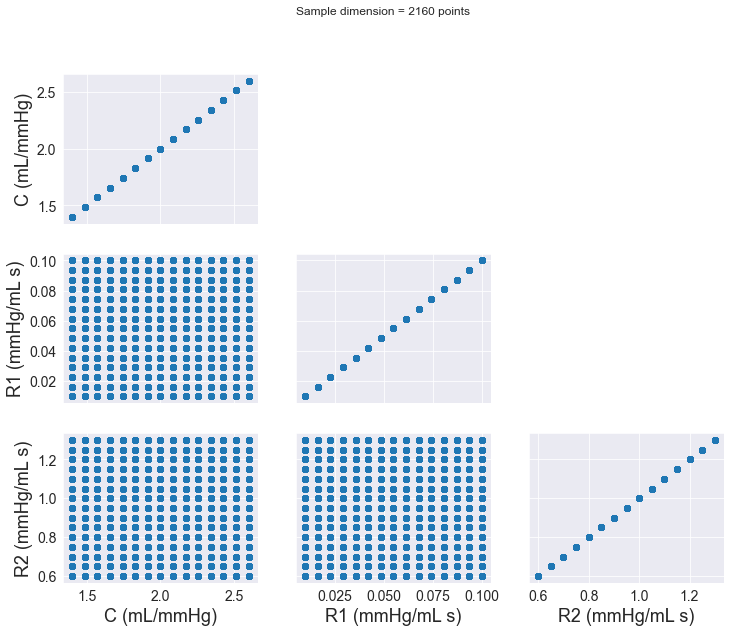
\includegraphics[width=1\textwidth]{images/Training (risultati)/database.png}
    \caption{Distribuzione dei dati nel database.}
    \label{distribuzioneDataset}
\end{figure}

\newpage
\section{Risultati del training}


%******************************
%*********** MAP **************
%******************************
\subsection{Mean arterial pressure (MAP)}
Viene impostato $\text{lr}=0.1$ e viene usato l'early stopper \textit{GLEarlyStoppingCriterion} con parametri: $\alpha = 5$, $\text{patience}=2$.


% **********
% MAP - loss
% **********
\subsubsection{Training e validation loss}
Il training ha necessitato cinquantadue EPOCHS (ogni EPOCH consiste in valutare il gradiente su ogni elemento del dataset), ha concluso con $\text{R2Score}=0.9999$, $\text{MeanSquaredError}=0.0001$. In figura \ref{MAP - loss} viene mostrato l'andamento del training e validation loss con MSE e R2Score; in verde l'andamento dell'early stopper.
\begin{figure}[h]
    \centering
    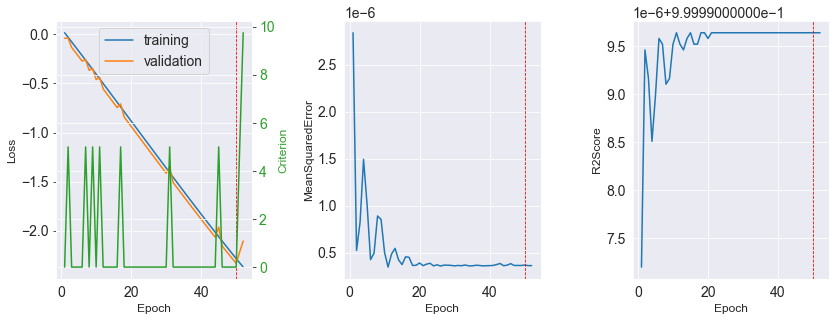
\includegraphics[width=1\textwidth]{images/Training (risultati)/MAP/MAP - loss.png}
    \caption{MAP: andamento del training e validation loss, early stopper, R2Score e MSE.}
    \label{MAP - loss}
\end{figure}

\newpage



% **********
% MAP - inference
% **********
\subsubsection{Approssimazione dei dati di input}
In figura \ref{MAP - inference} viene mostrato come le predizioni approssimano i dati di input. La lunghezza delle barre di errore è $0.0015$, quindi sono molto corte indicando un'alta precisione.

\begin{figure}[!htb]
    \centering
    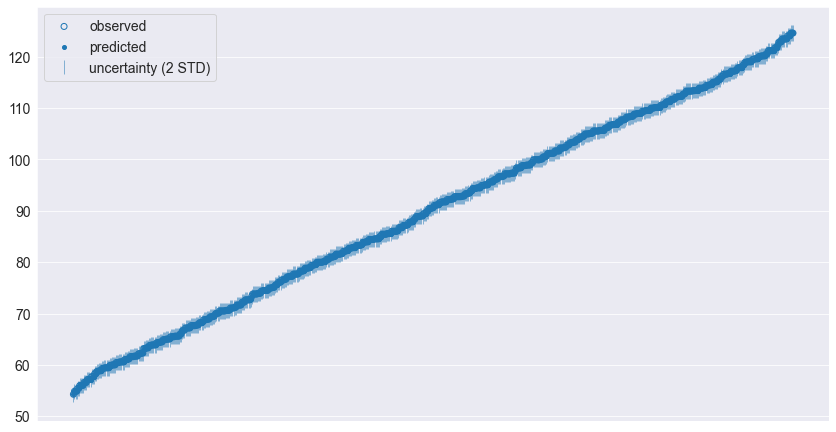
\includegraphics[width=1\textwidth]{images/Training (risultati)/MAP/MAP - inference.png}
    \caption{MAP: predizioni sui dati di input.}
    \label{MAP - inference}
\end{figure}



% **********
% MAP - C
% **********
\subsubsection{Dipendenza da $C$}
Per studiare la dipendenza di MAP da $C$, vengono presi novanta valori di $C$ equidistanziati nello stesso intervallo usato per la creazione del database di input e, fissati i valori di $R_1$ e $R_2$ a quelli trovati nella loro approssimazione in \ref{stimaCR}, viene generato un file di combinazioni $C$, $R_1$ e $R_2$. Per ogni combinazione viene trovata l'approssimazione della pressione con il modello Windkessel e calcolata la MAP; con la combinazione di compliance e resistenze viene poi stimata la MAP usando il modello già addestrato. Viene poi fatto lo stesso su due intervalli attigui a quello di training e ampi il $10\%$ dell'intervallo di training. Il risultato complessivo è mostrato in figura \ref{MAP - C - full}, il risultato nel solo intervallo di training in \ref{MAP - C - training}, il risultato nei singoli intervalli attigui in \ref{MAP - C - sx} e \ref{MAP - C - dx}.

\begin{figure}
    \centering
    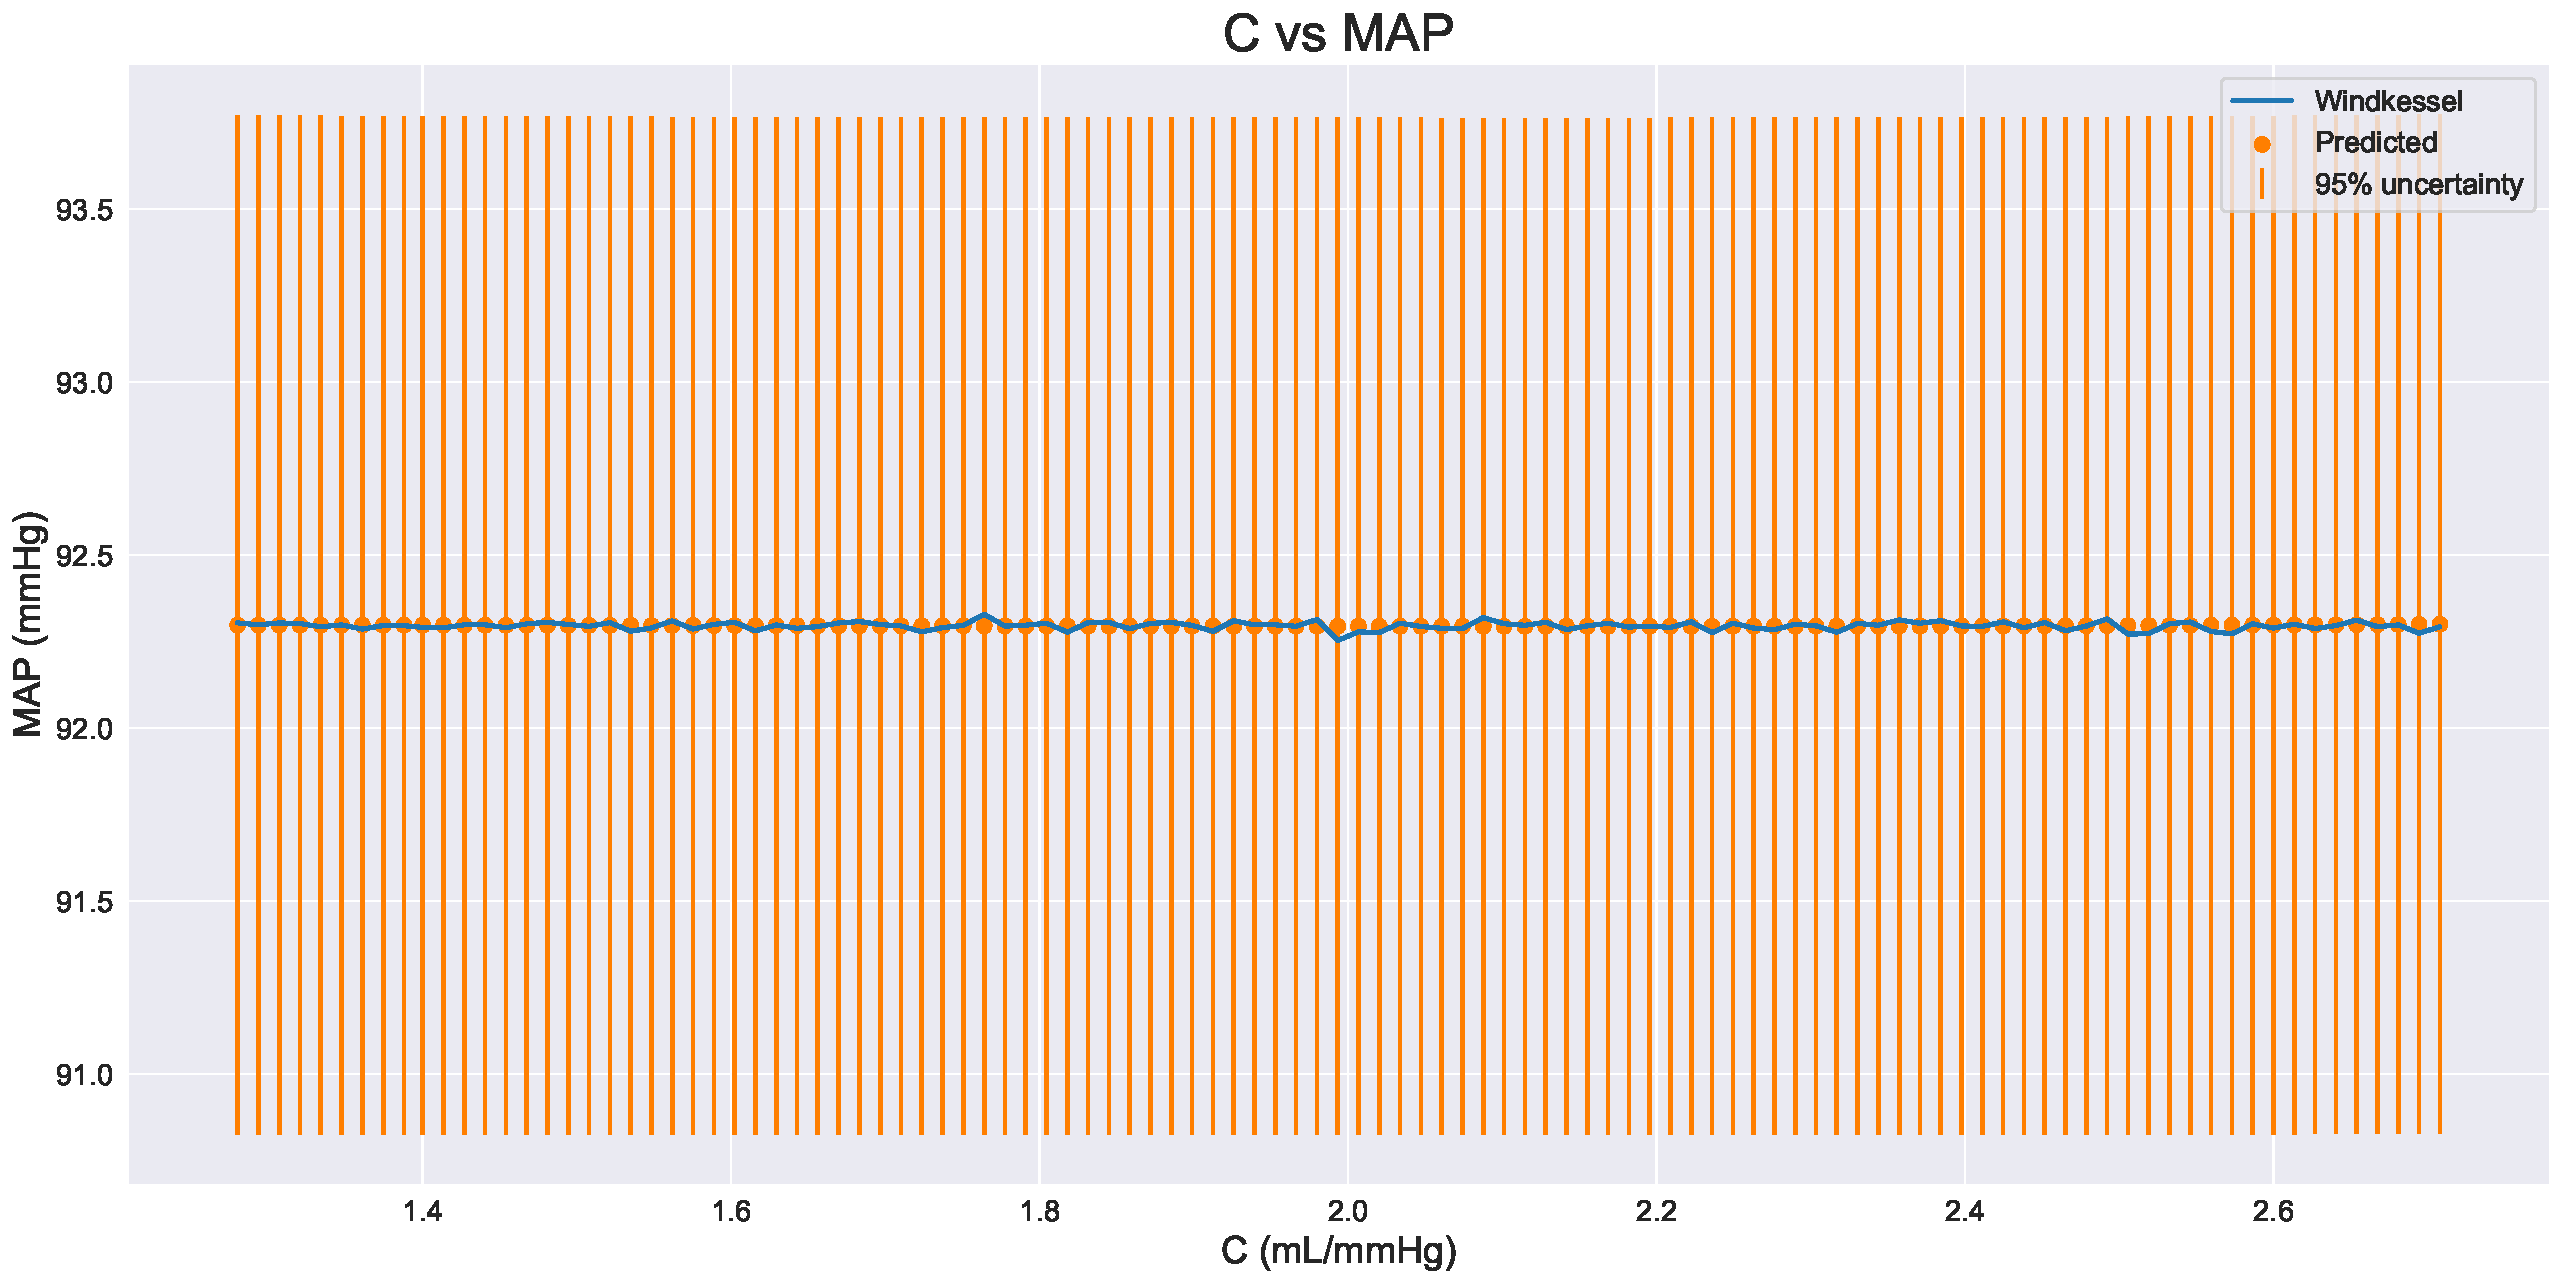
\includegraphics[width=1\textwidth]{images/Training (risultati)/MAP/MAP - C - full.pdf}
    \caption{Dipendenza di MAP da $C$ sull'intervallo di training e due intervalli attigui.}
    \label{MAP - C - full}
\end{figure}


\begin{figure}
    \centering
    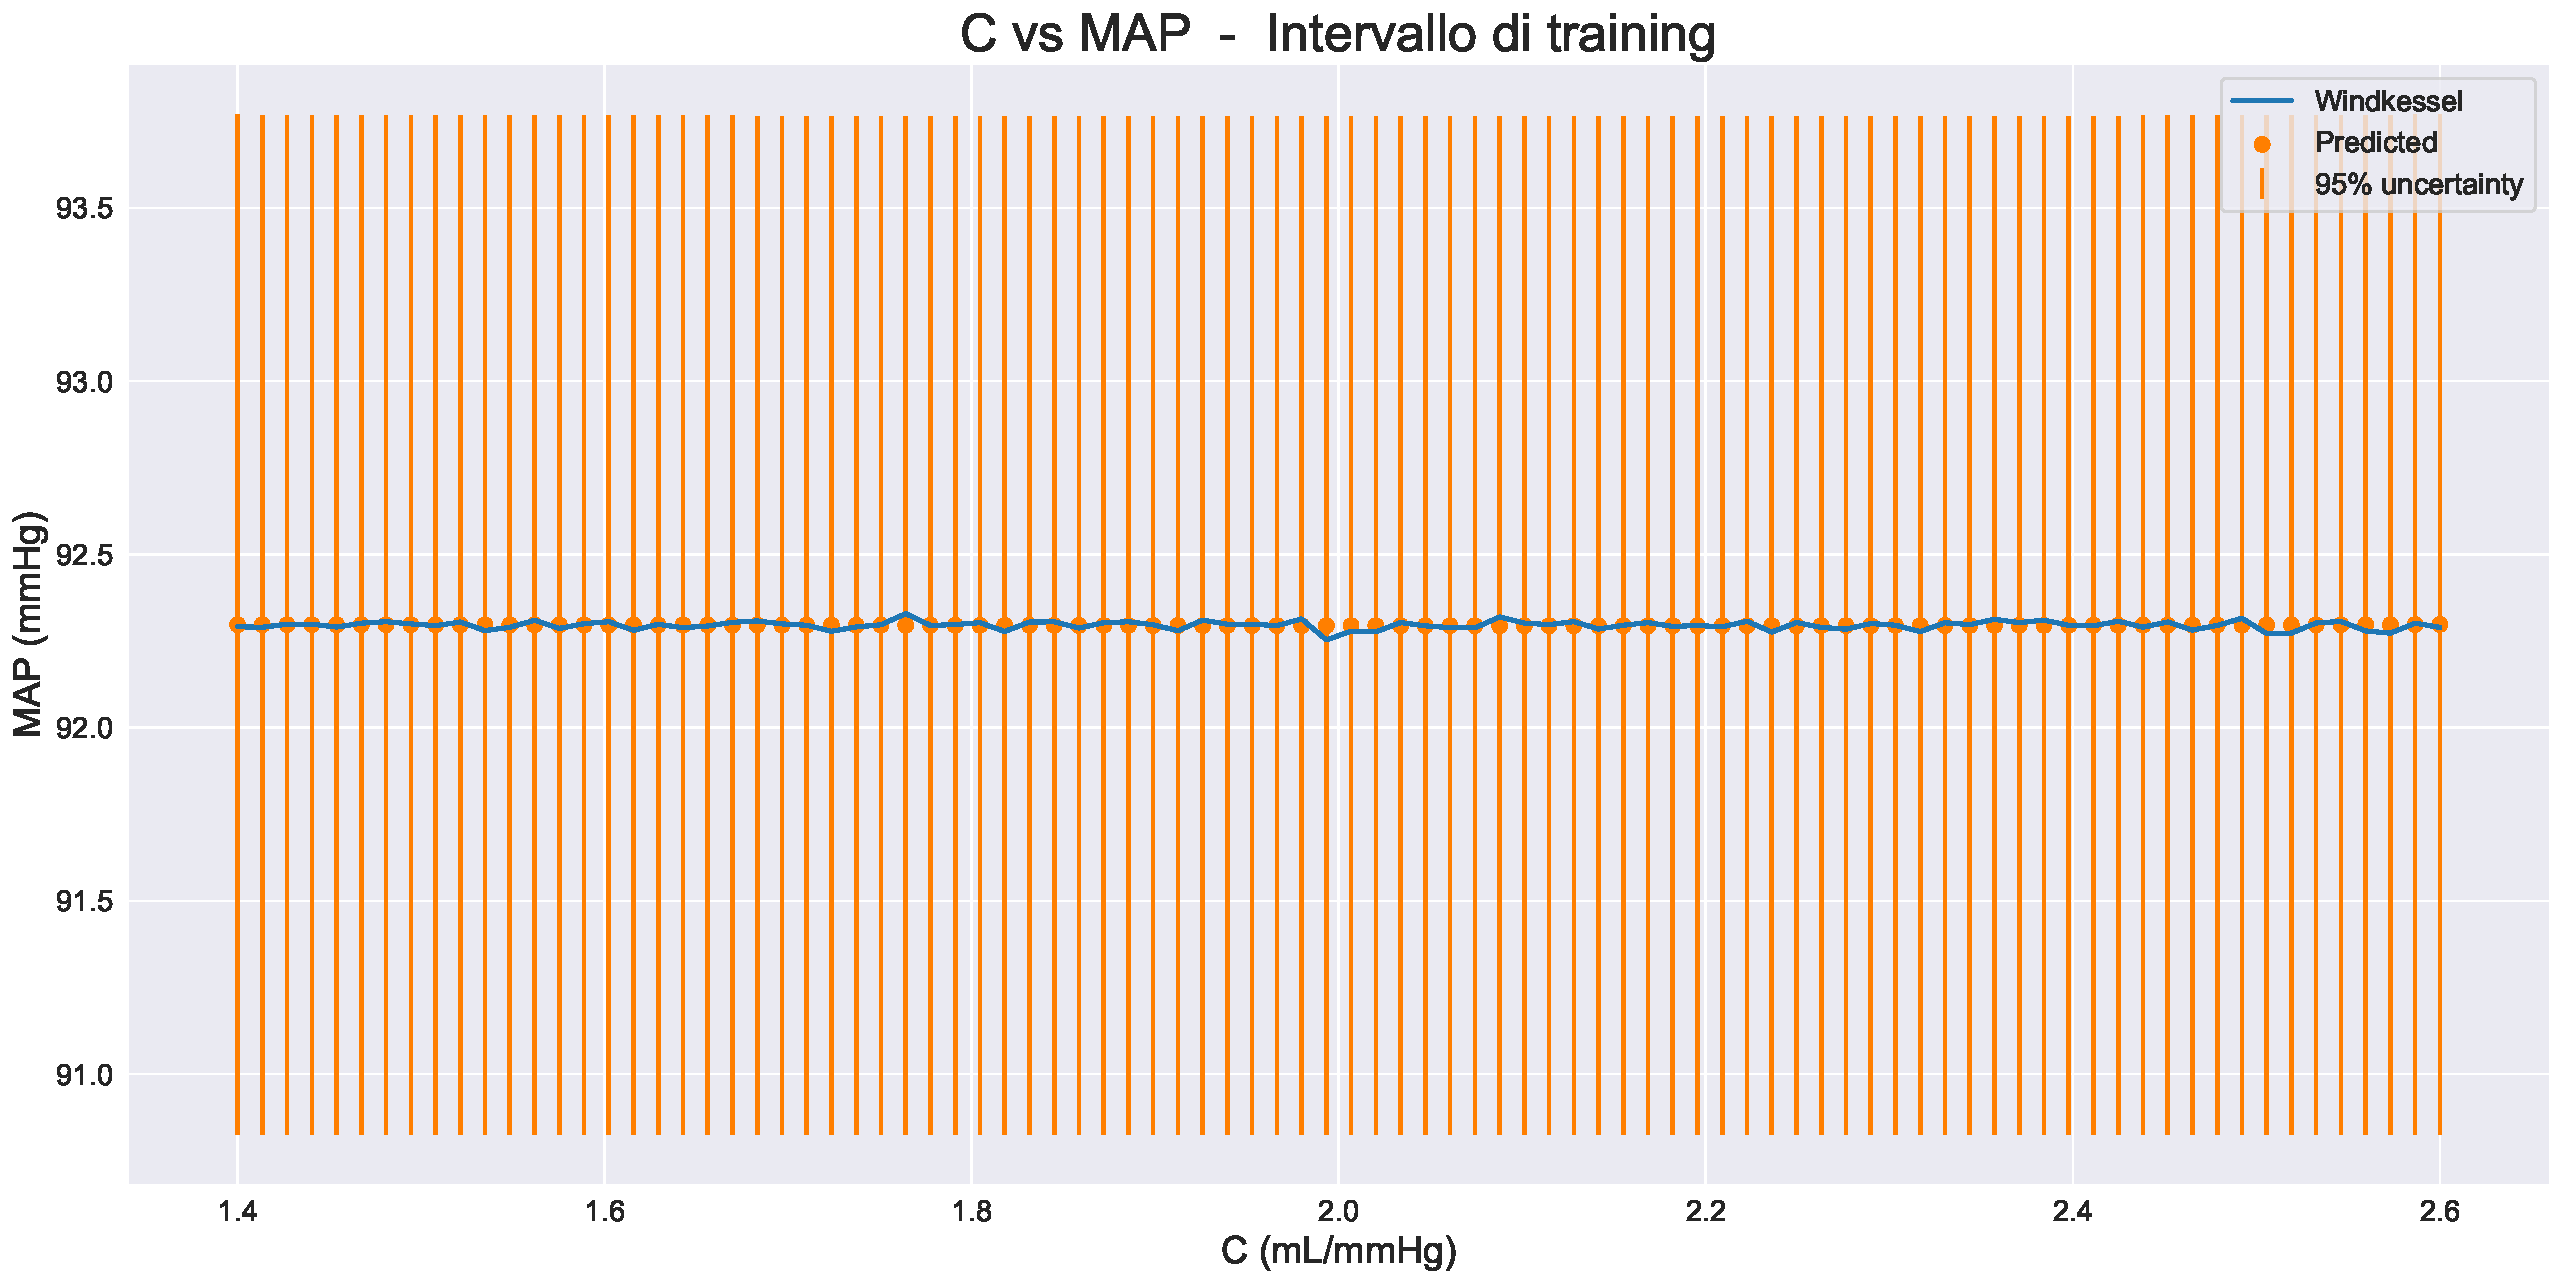
\includegraphics[width=1\textwidth]{images/Training (risultati)/MAP/MAP - C - training.pdf}
    \caption{Dipendenza di MAP da $C$ sull'intervallo di training.}
    \label{MAP - C - training}
\end{figure}


\begin{figure}
    \centering
    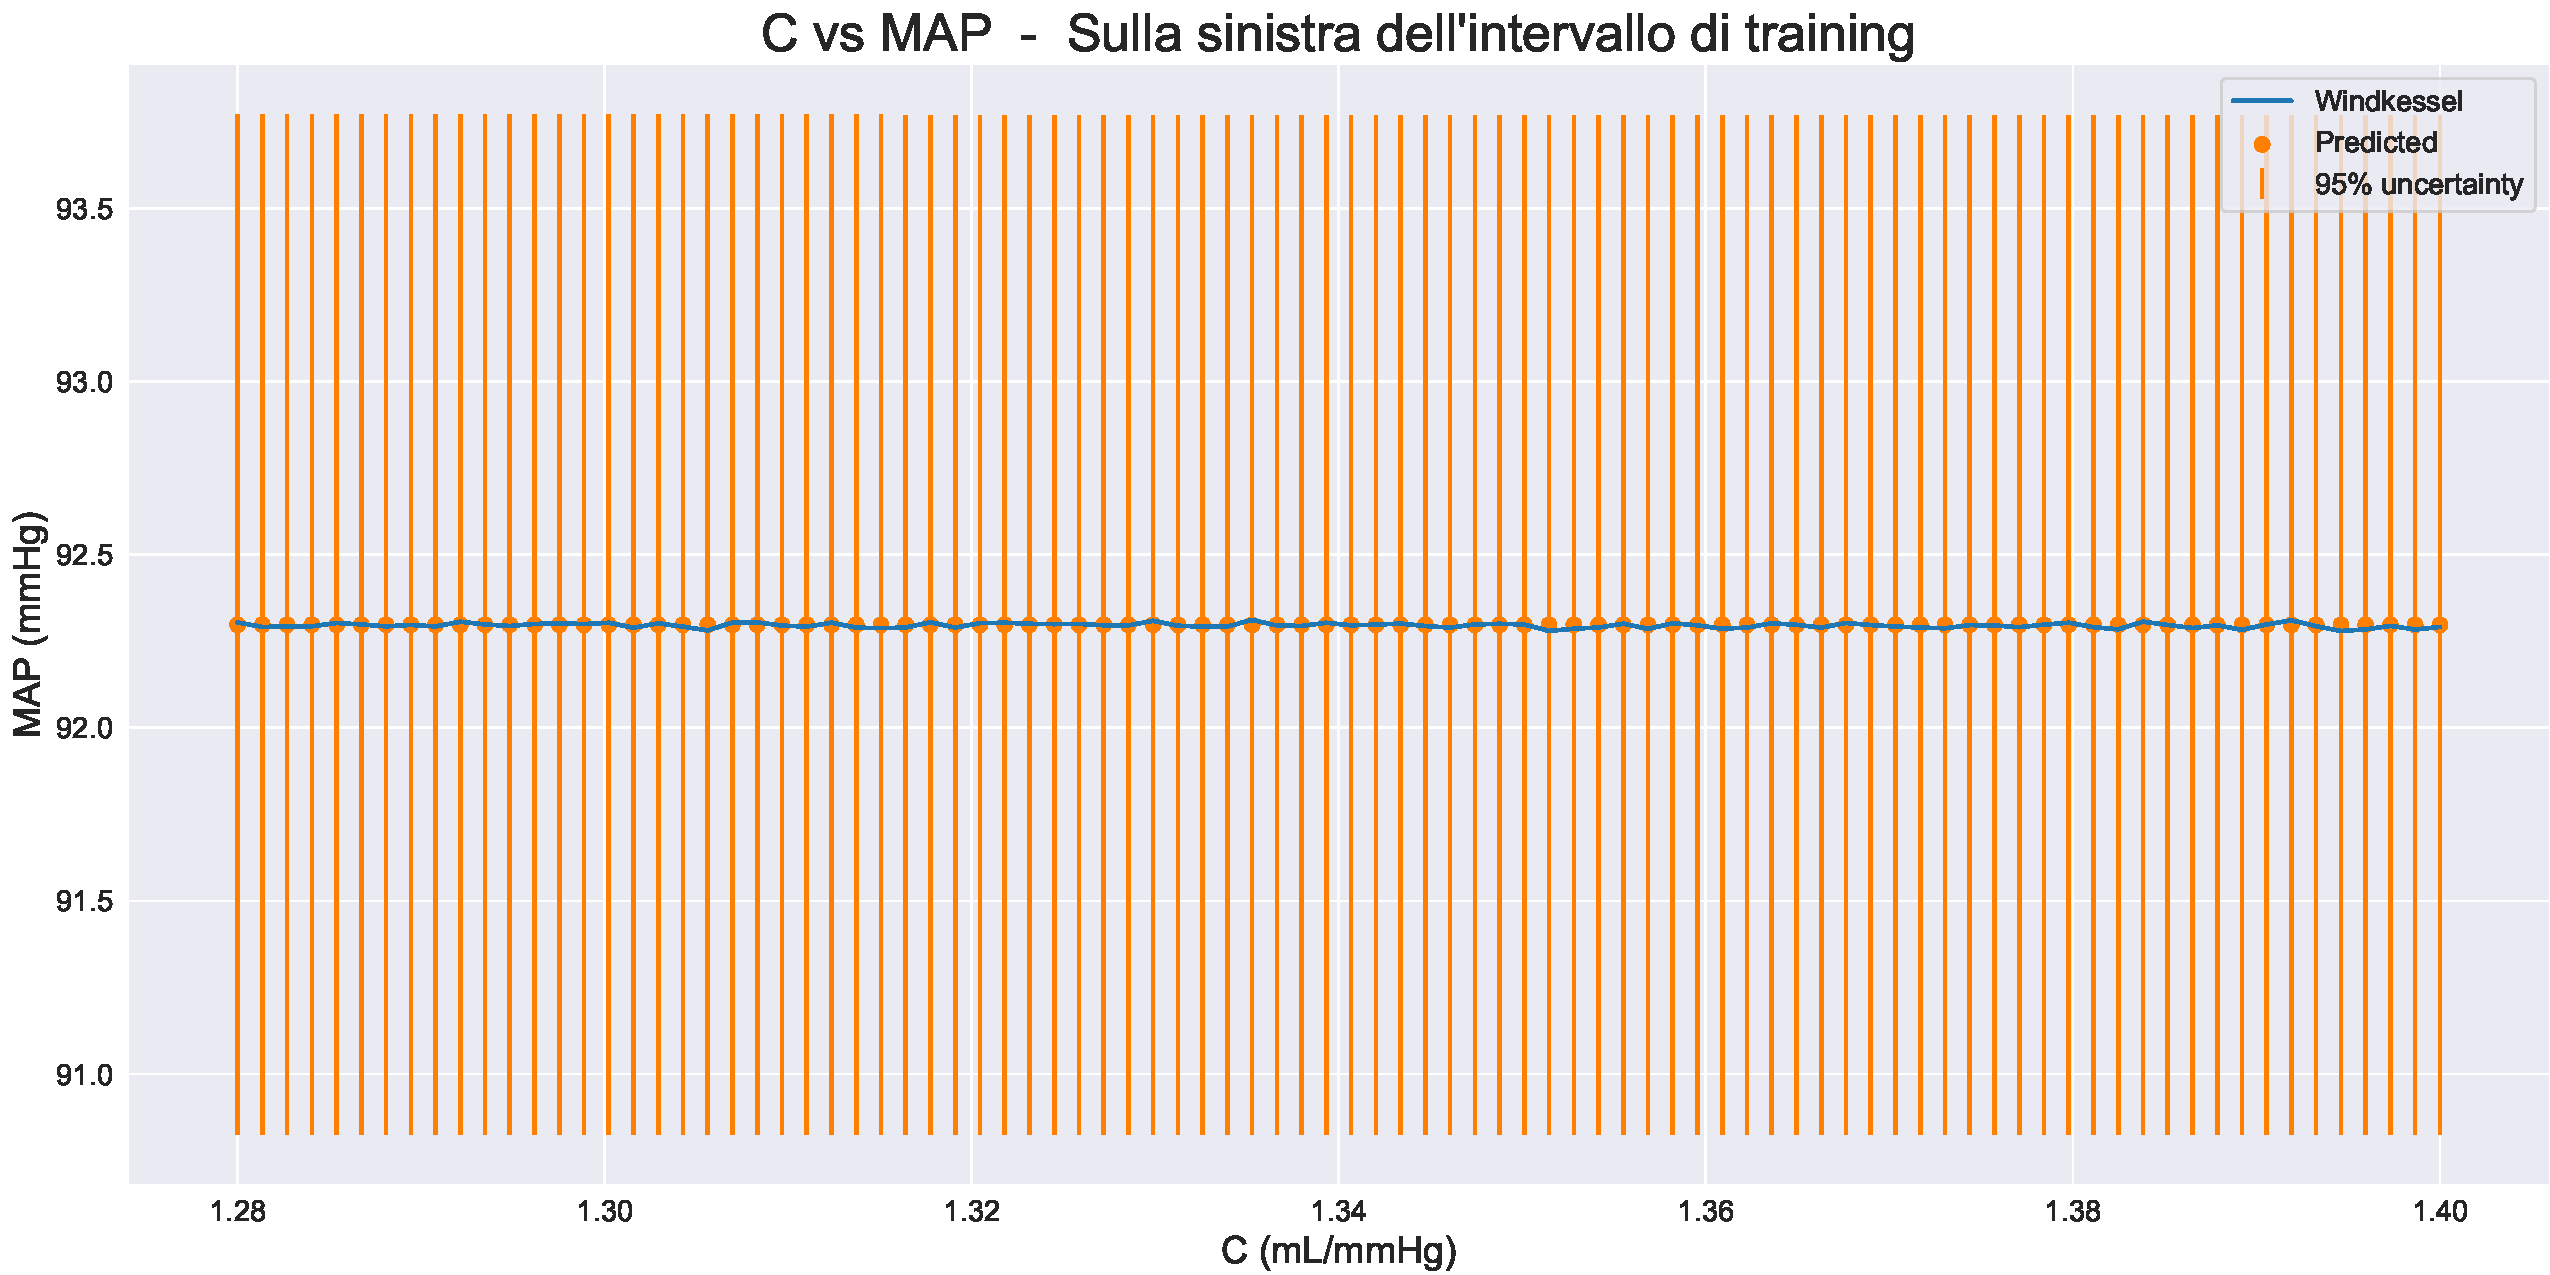
\includegraphics[width=1\textwidth]{images/Training (risultati)/MAP/MAP - C - sx.pdf}
    \caption{Dipendenza di MAP da $C$ sull'intervallo attiguo a sinistra dell'intervallo di training.}
    \label{MAP - C - sx}
\end{figure}



\begin{figure}
    \centering
    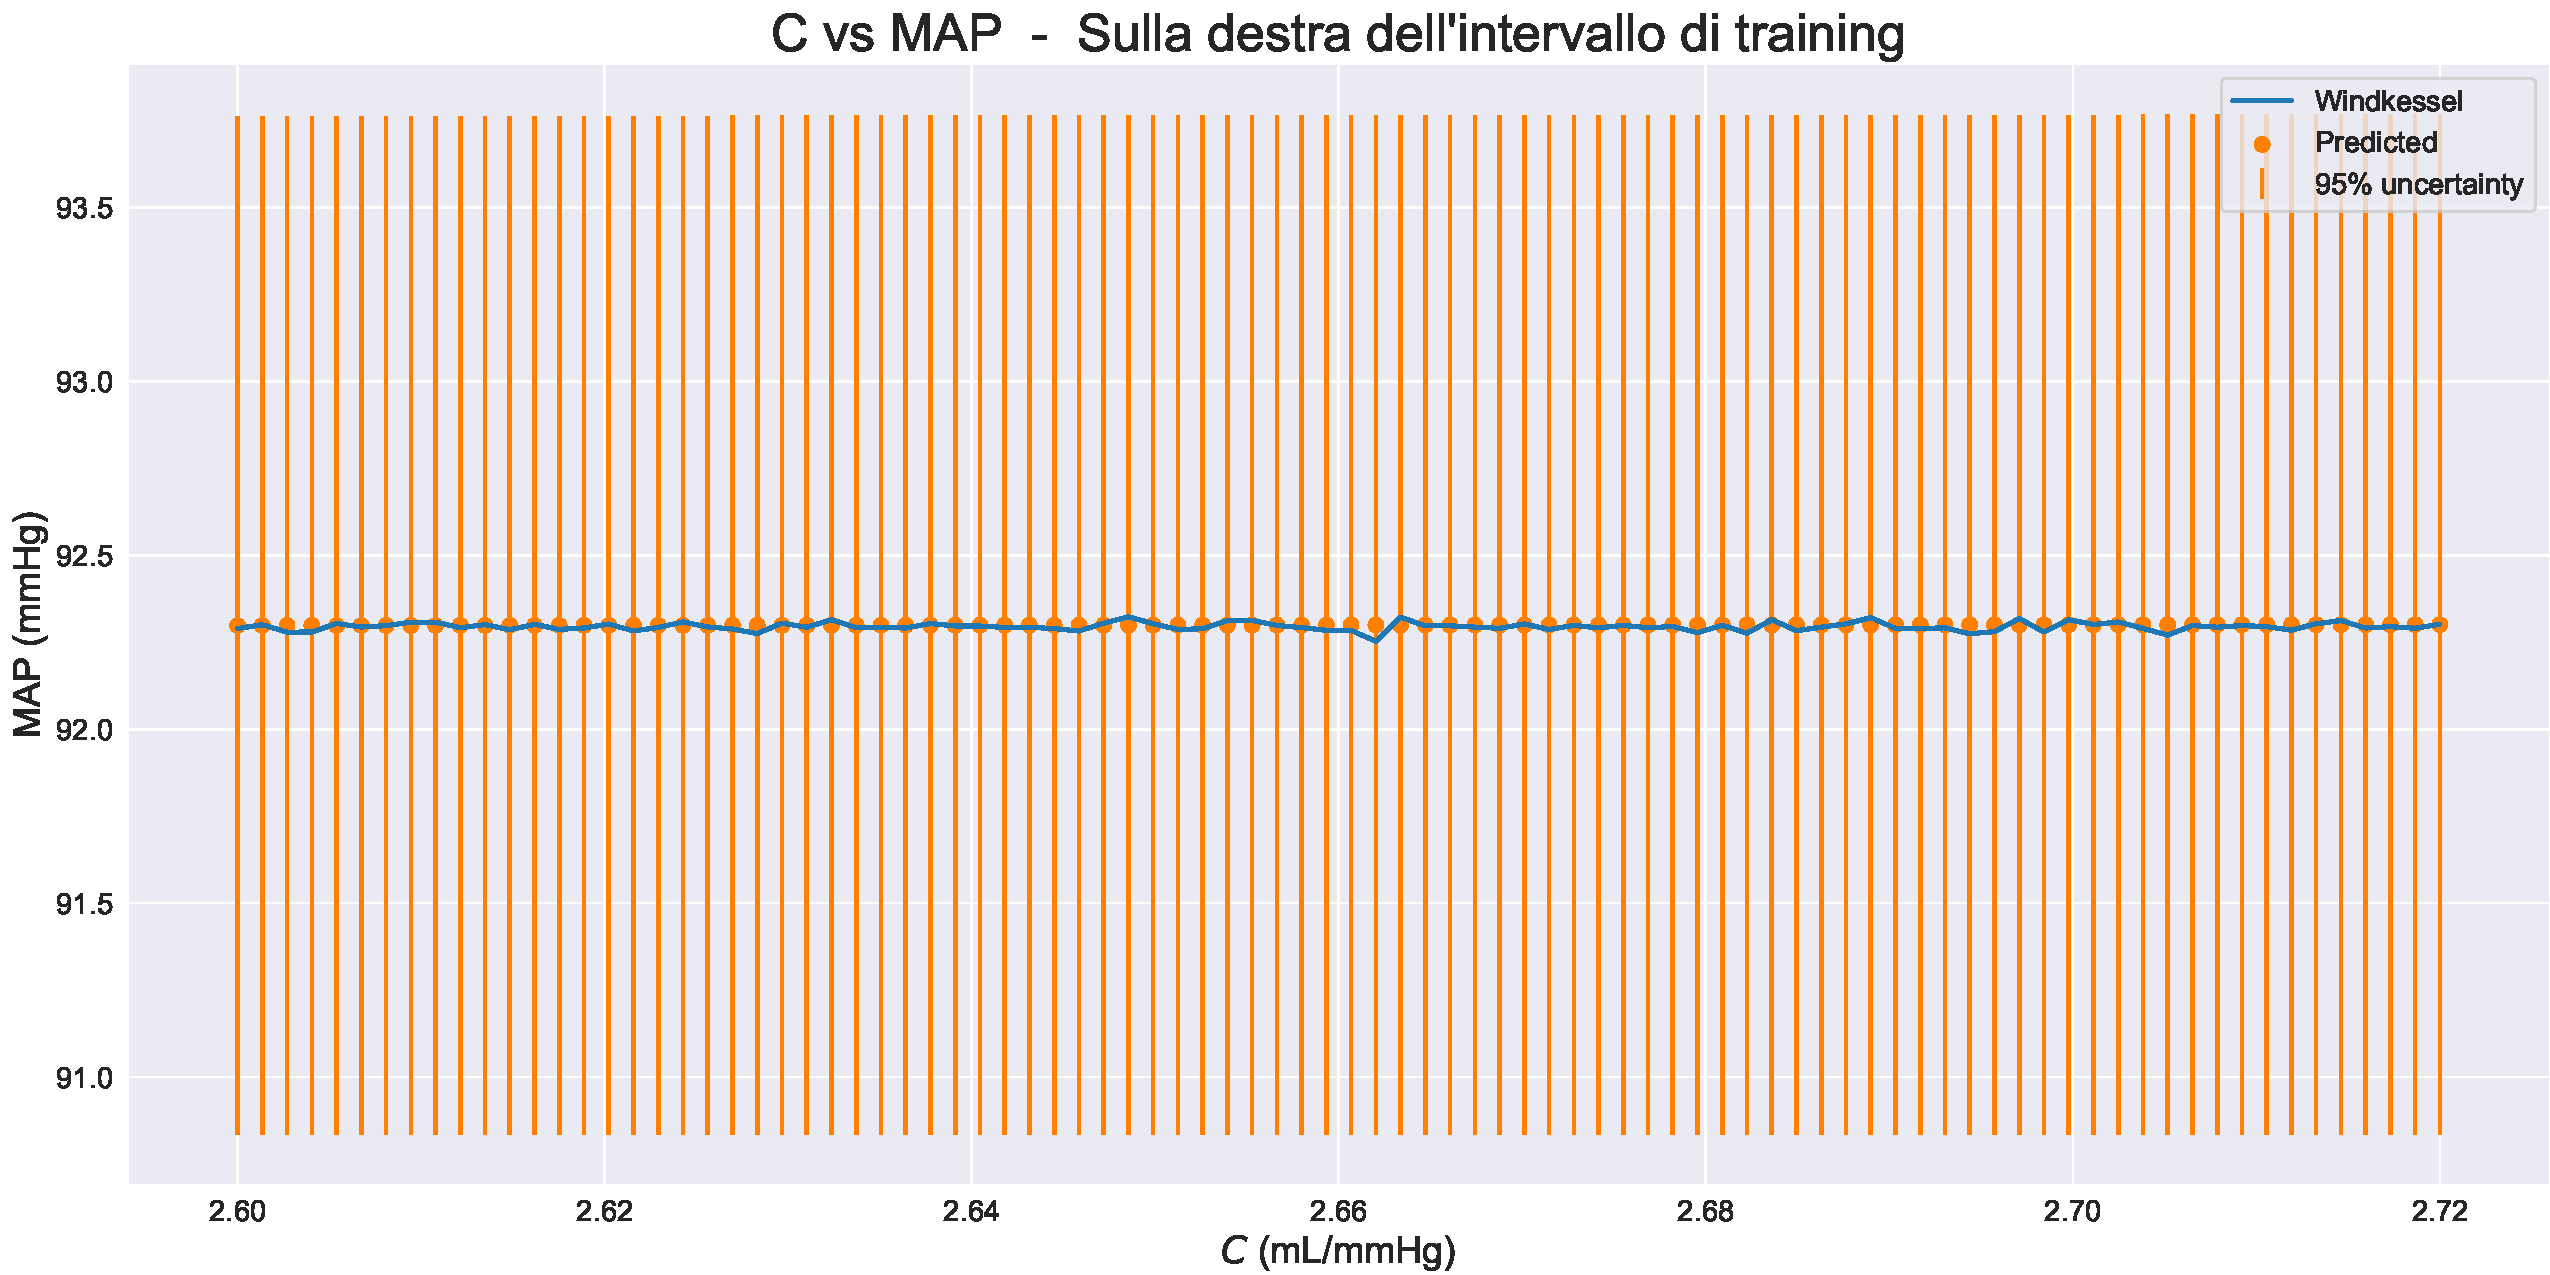
\includegraphics[width=1\textwidth]{images/Training (risultati)/MAP/MAP - C - dx.pdf}
    \caption{Dipendenza di MAP da $C$ sull'intervallo attiguo a destra dell'intervallo di training.}
    \label{MAP - C - dx}
\end{figure}




\newpage
% **********
% MAP - R1
% **********
\subsubsection{Dipendenza da $R_1$}
Per studiare la dipendenza da $R_1$ viene usato lo stesso approccio. Il risultato complessivo è mostrato in figura \ref{MAP - R1 - full}, il risultato nel solo intervallo di training in \ref{MAP - R1 - training}, il risultato nei singoli intervalli attigui in \ref{MAP - R1 - sx} e \ref{MAP - R1 - dx}.

\begin{figure}[!htb]
    \centering
    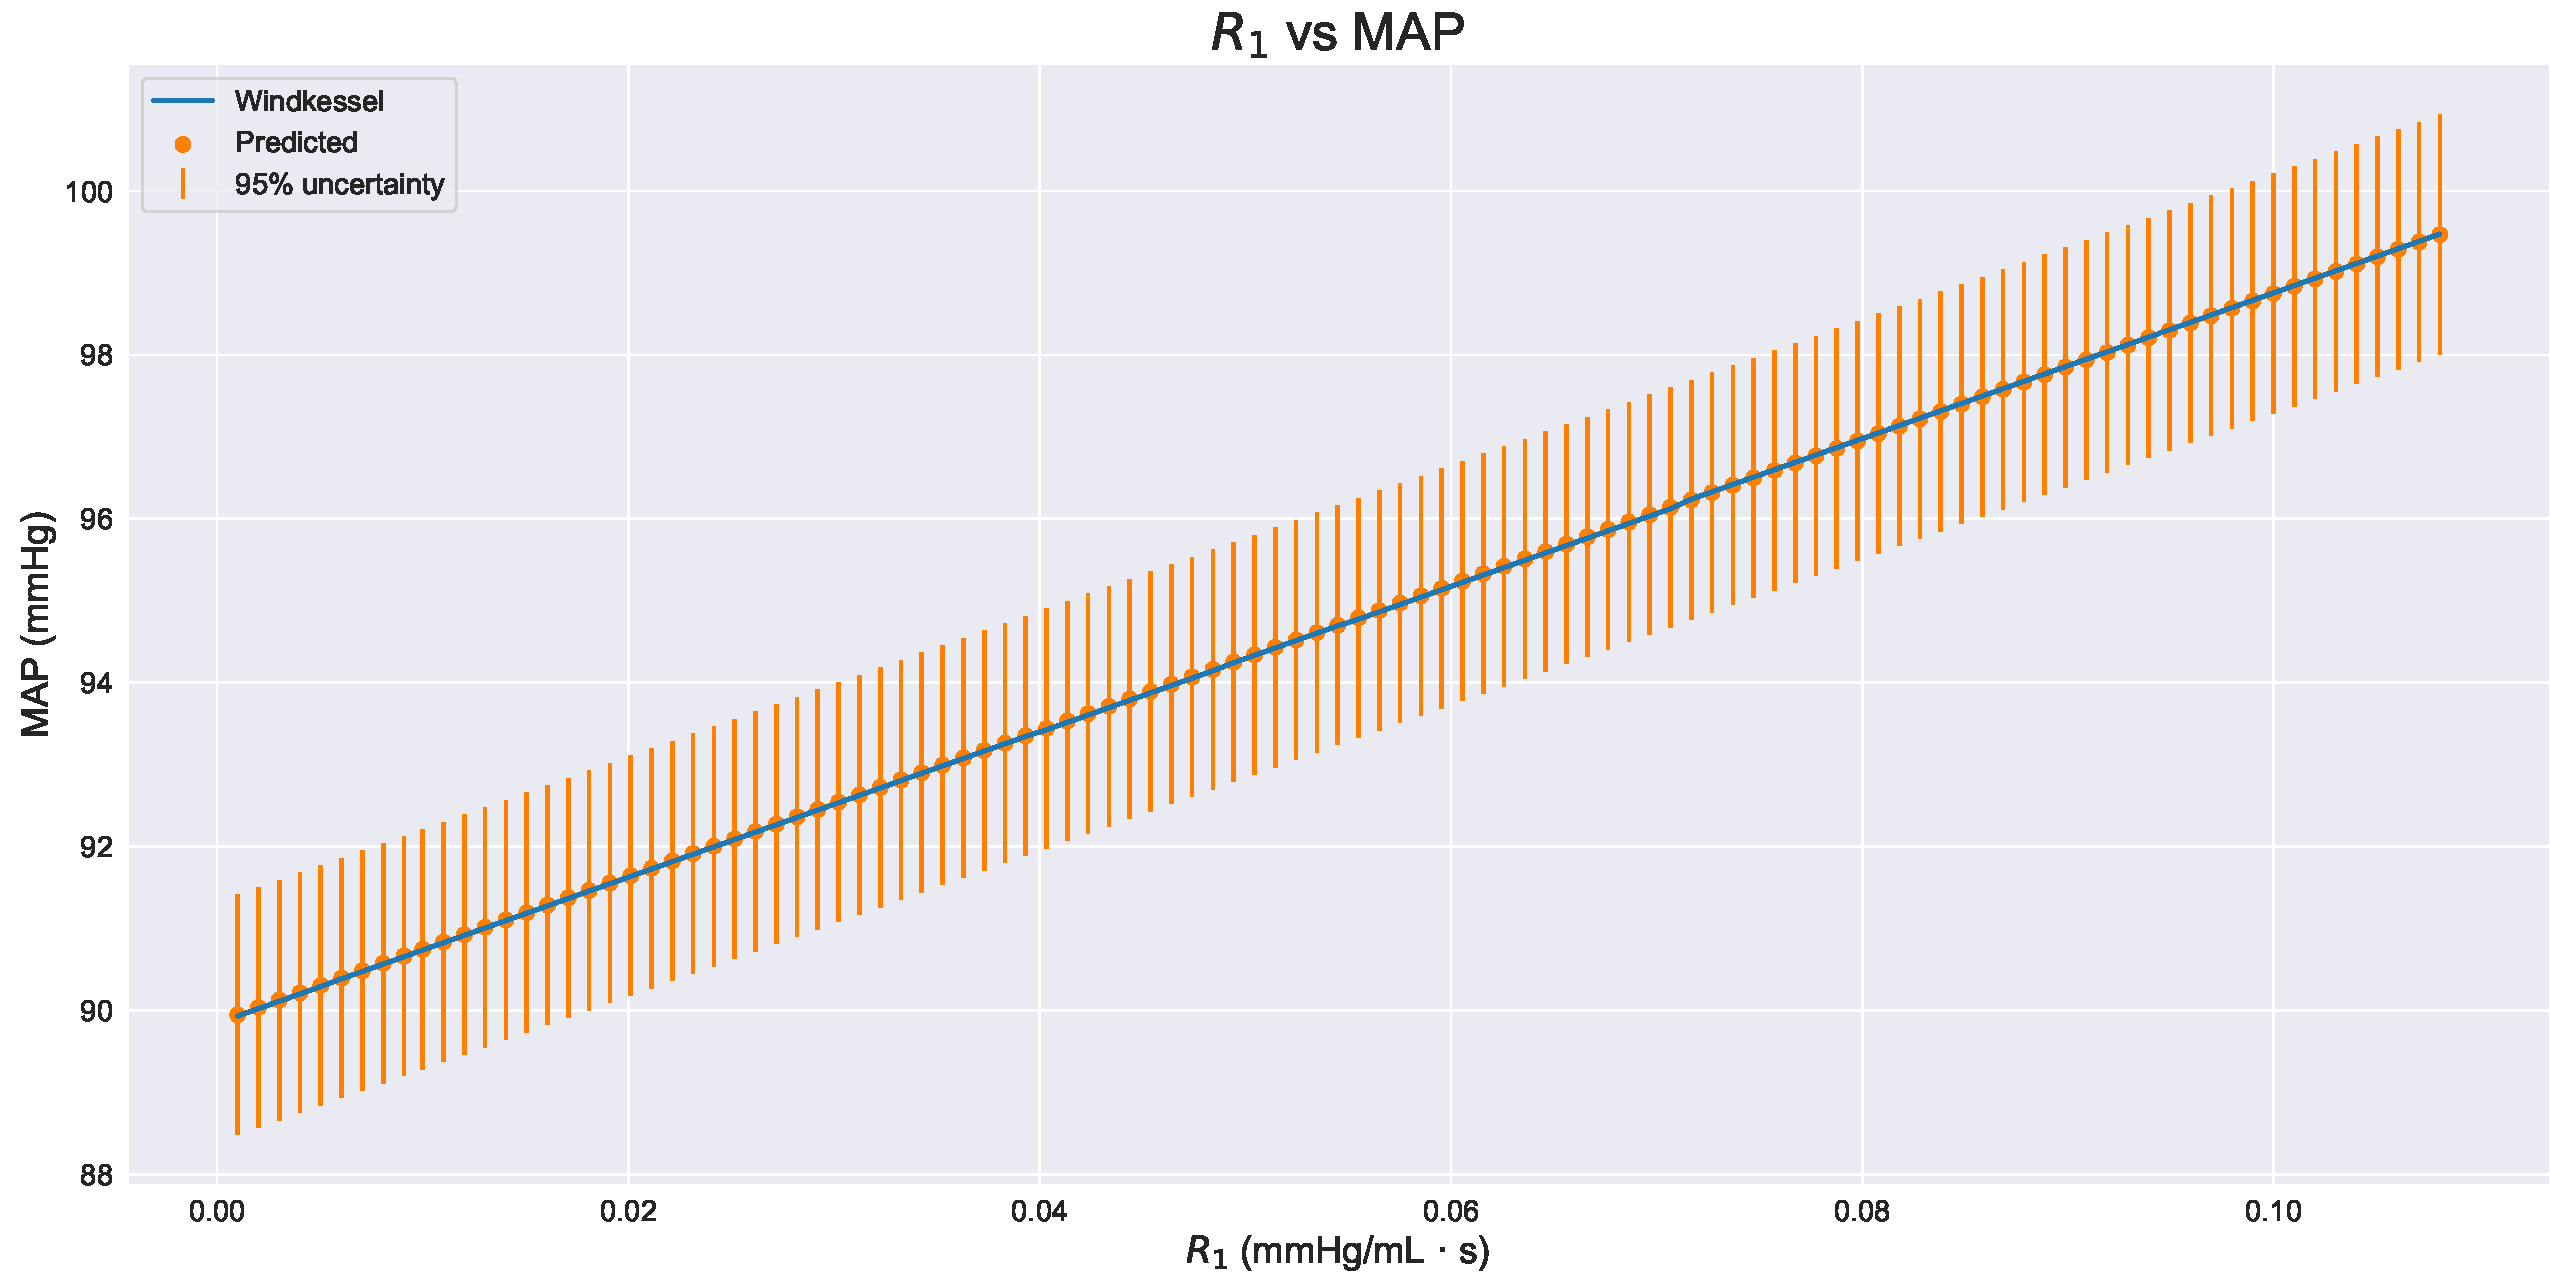
\includegraphics[width=1\textwidth]{images/Training (risultati)/MAP/MAP - R1 - full.pdf}
    \caption{Dipendenza di MAP da $R1$ sull'intervallo di training e due intervalli attigui.}
    \label{MAP - R1 - full}
\end{figure}

\vspace{1cm}

\begin{figure}[!htb]
    \centering
    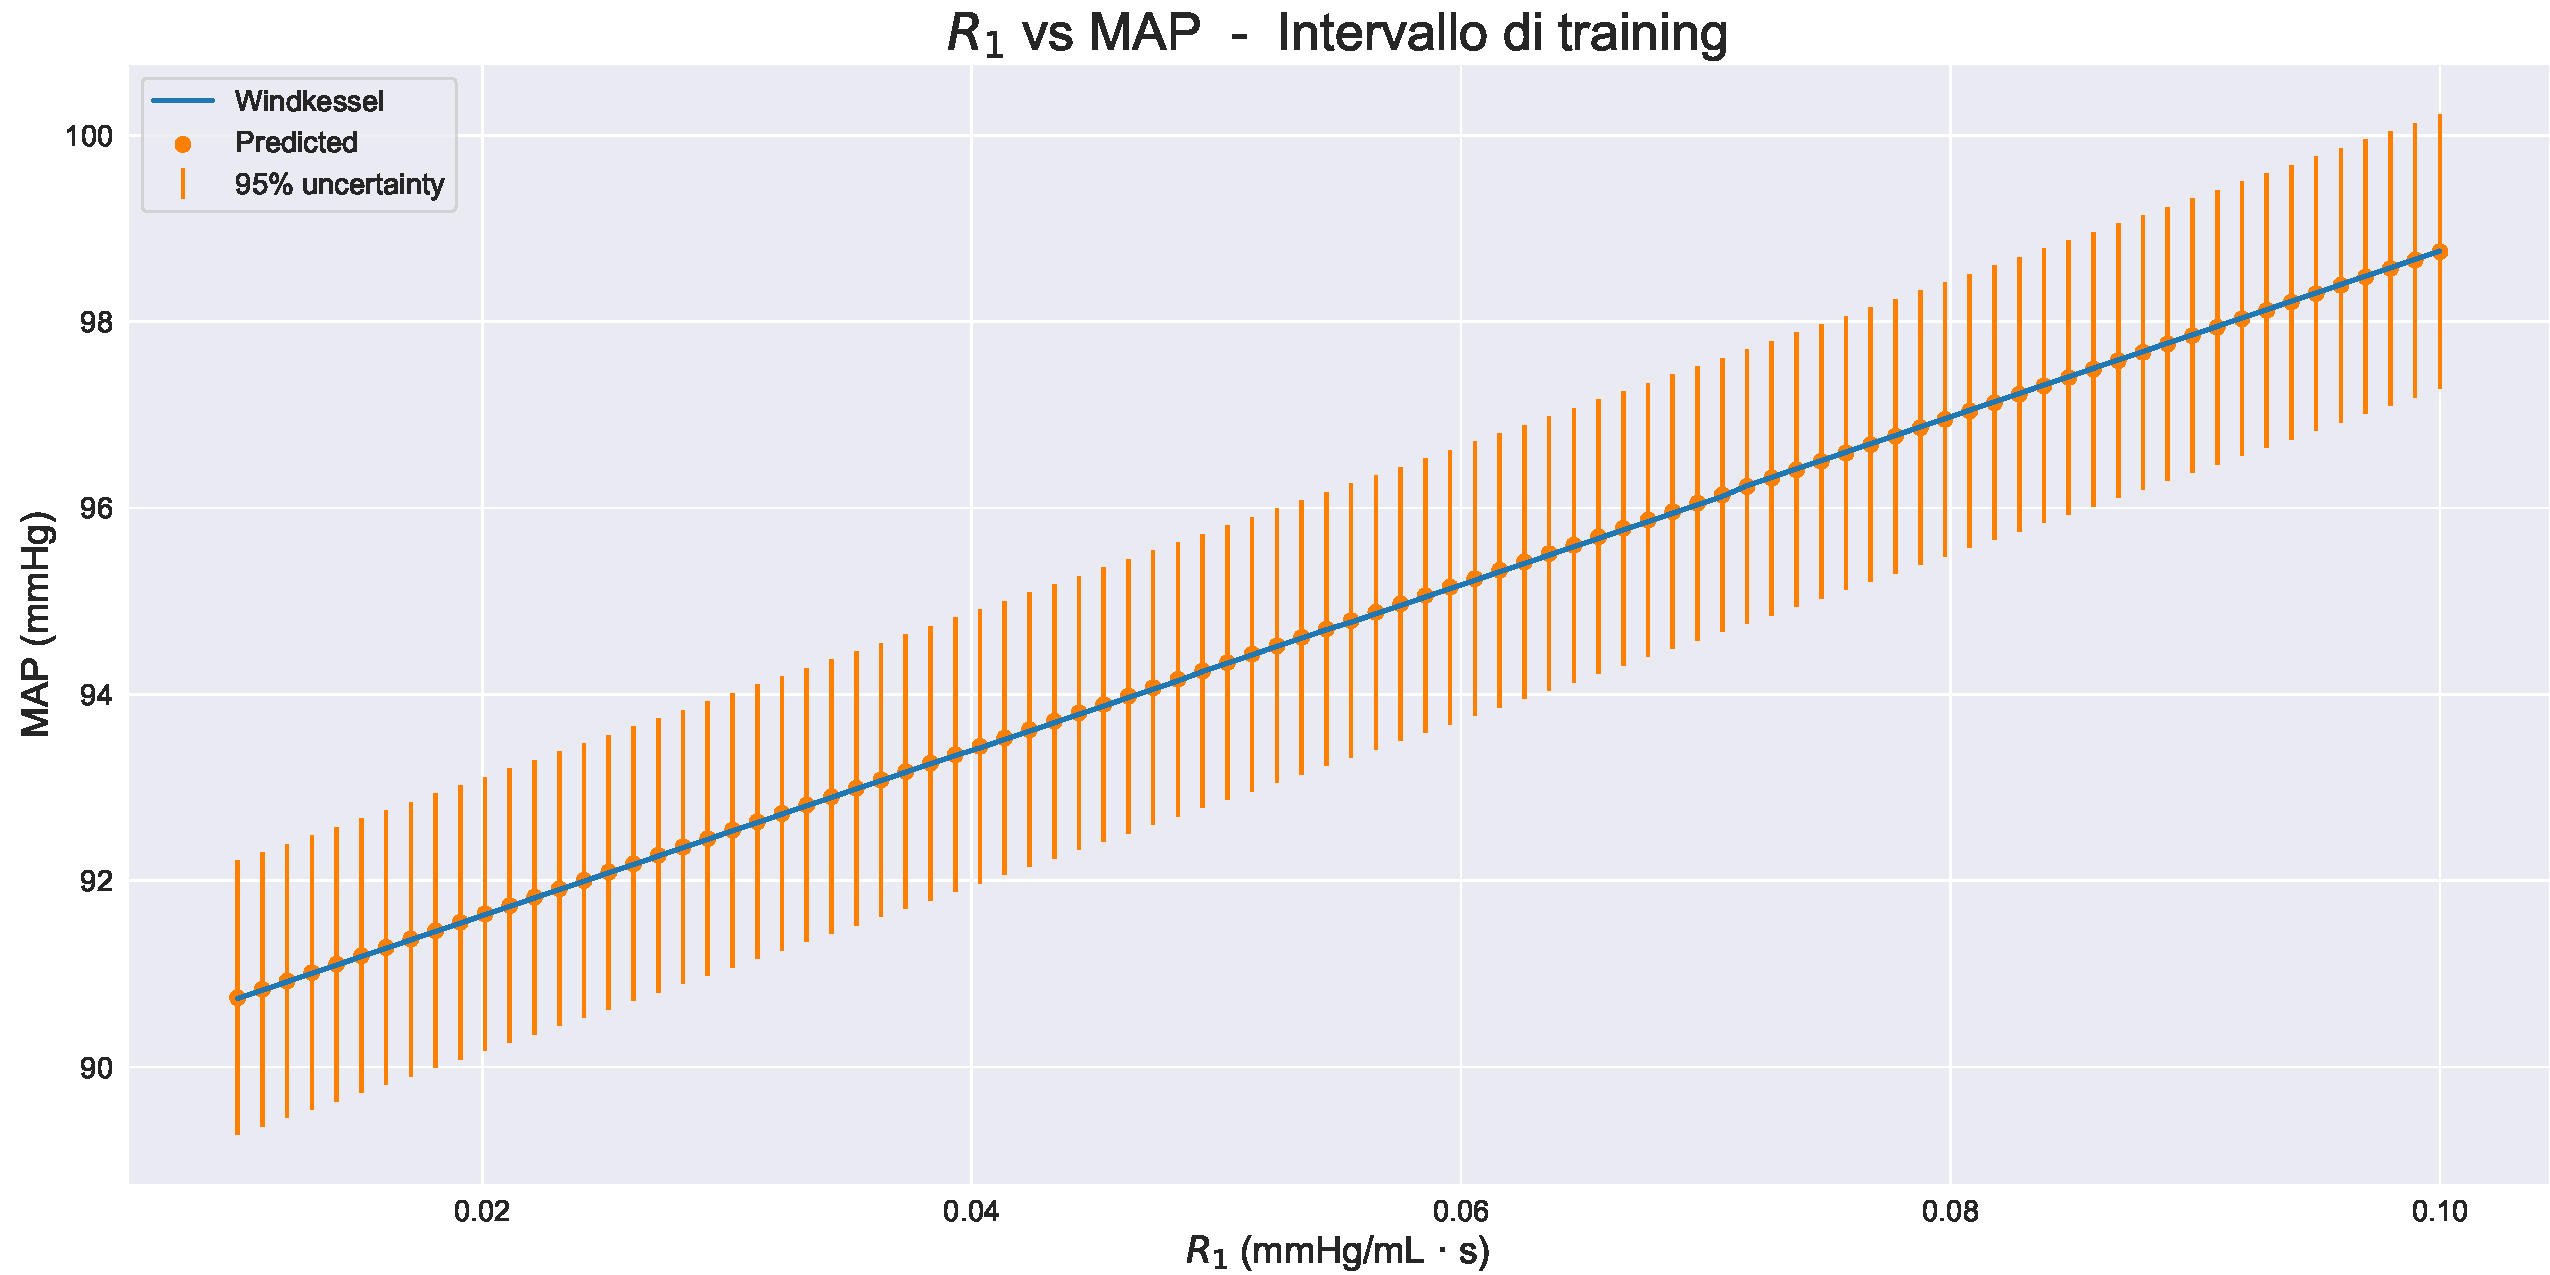
\includegraphics[width=1\textwidth]{images/Training (risultati)/MAP/MAP - R1 - training.pdf}
    \caption{Dipendenza di MAP da $R1$ sull'intervallo di training.}
    \label{MAP - R1 - training}
\end{figure}

\begin{figure}
    \centering
    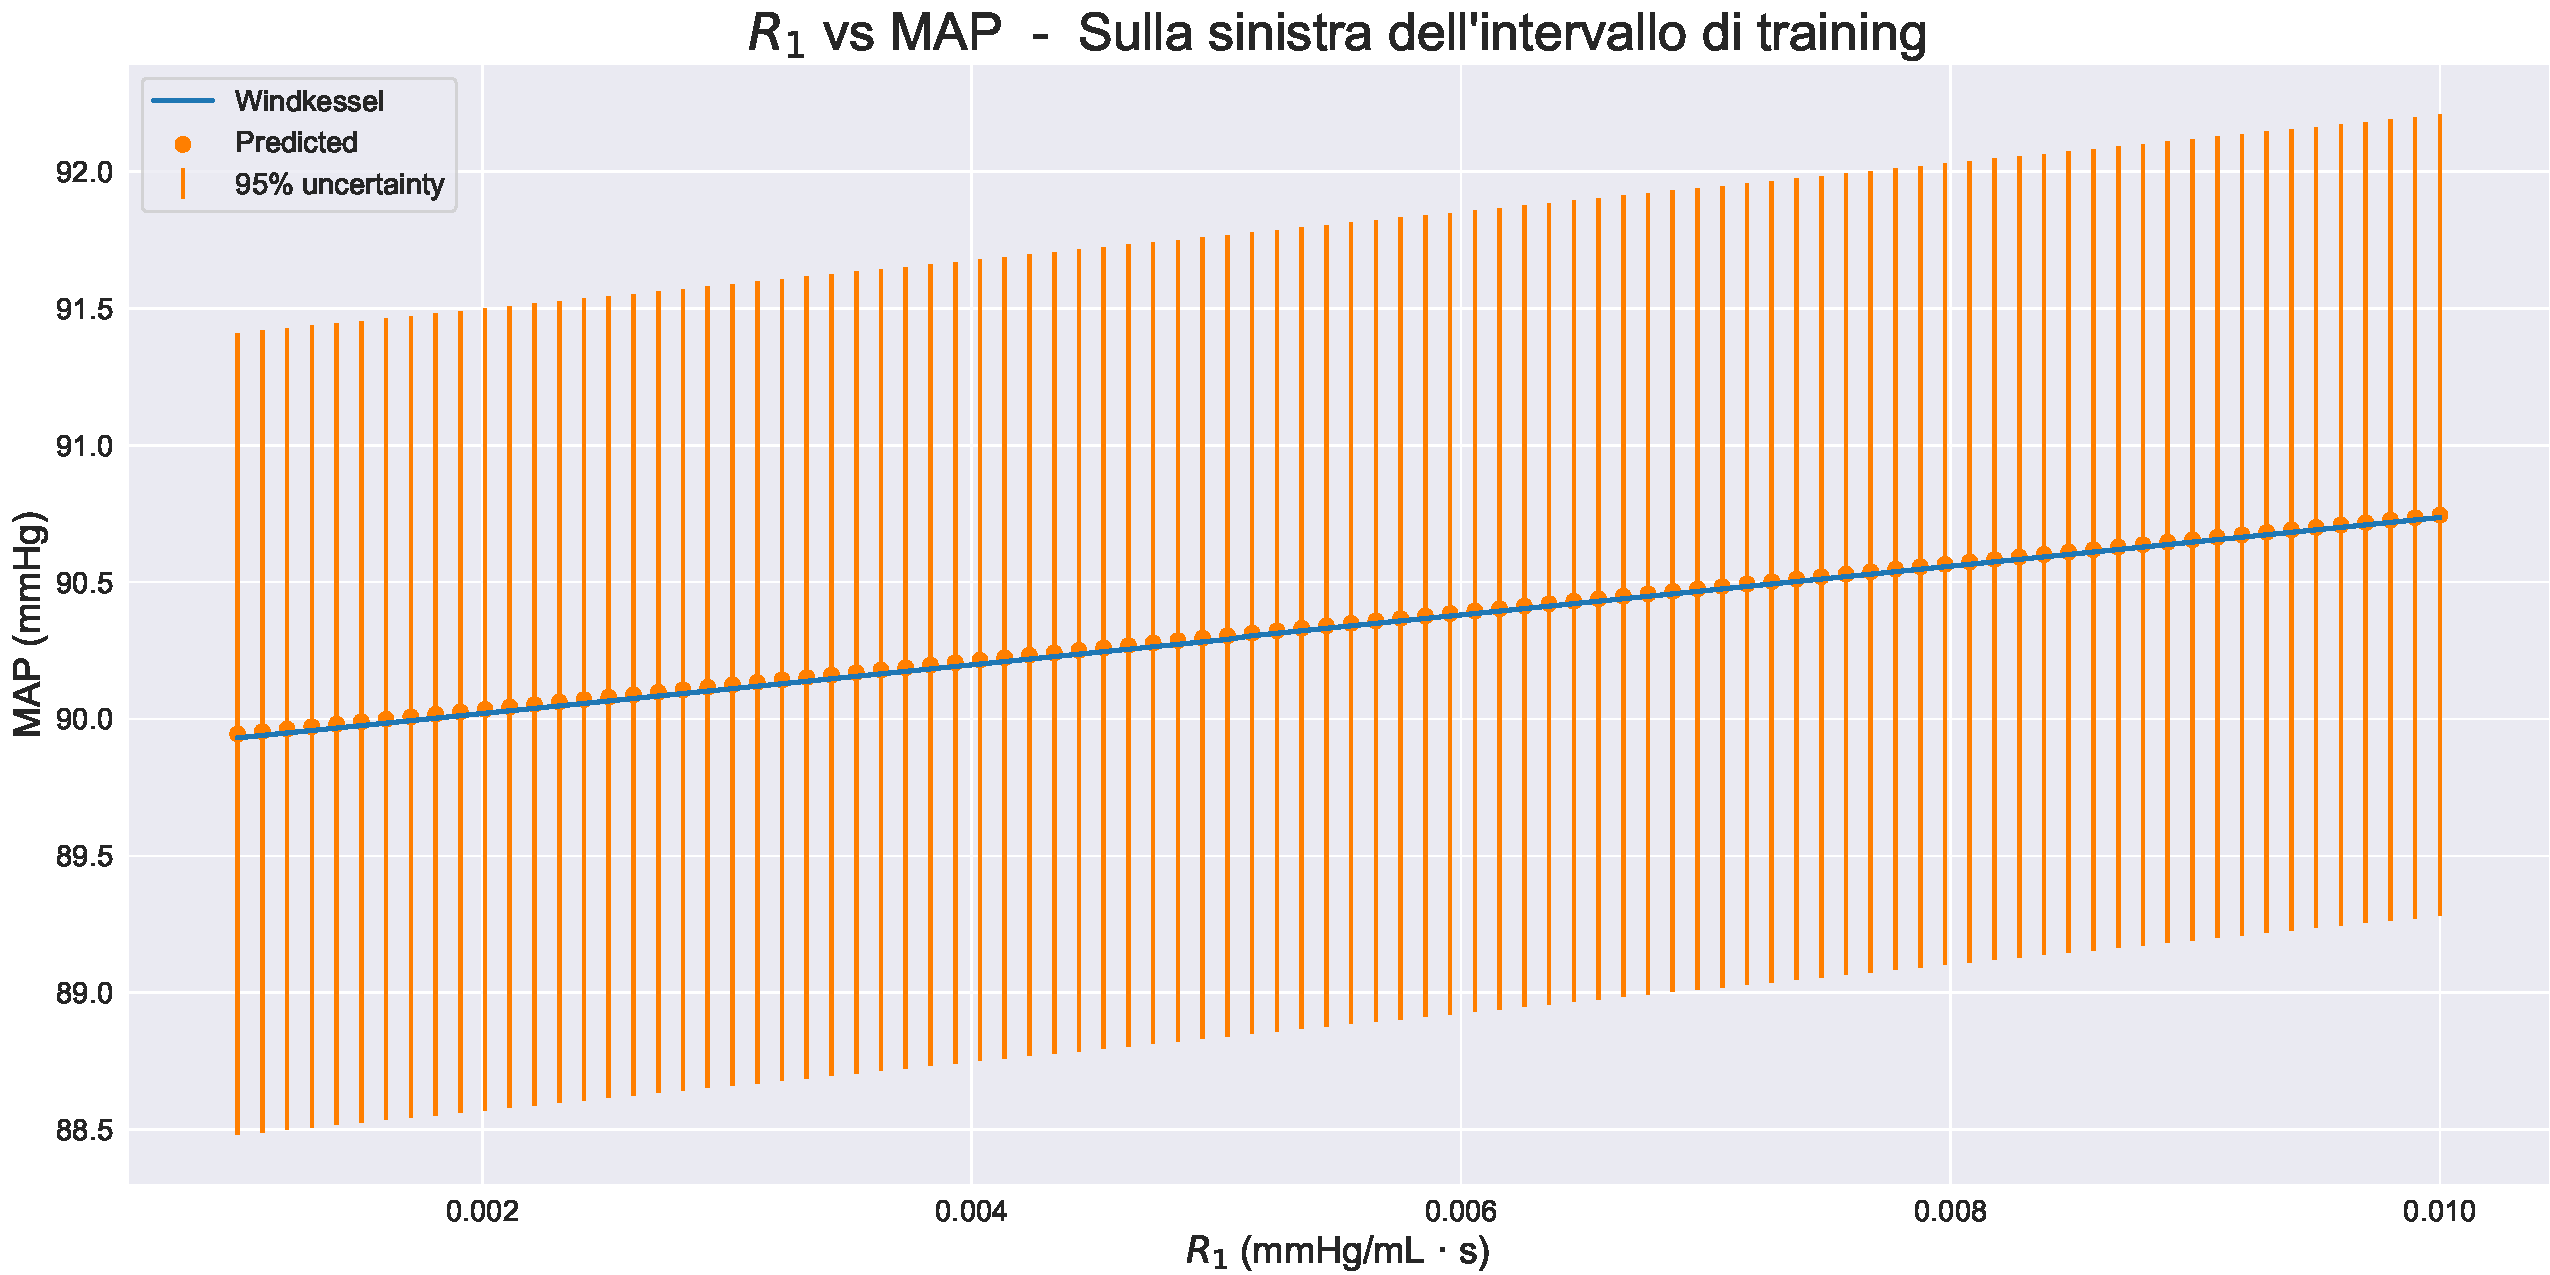
\includegraphics[width=1\textwidth]{images/Training (risultati)/MAP/MAP - R1 - sx.pdf}
    \caption{Dipendenza di MAP da $R1$ sull'intervallo attiguo a sinistra dell'intervallo di training.}
    \label{MAP - R1 - sx}
\end{figure}


\begin{figure}
    \centering
    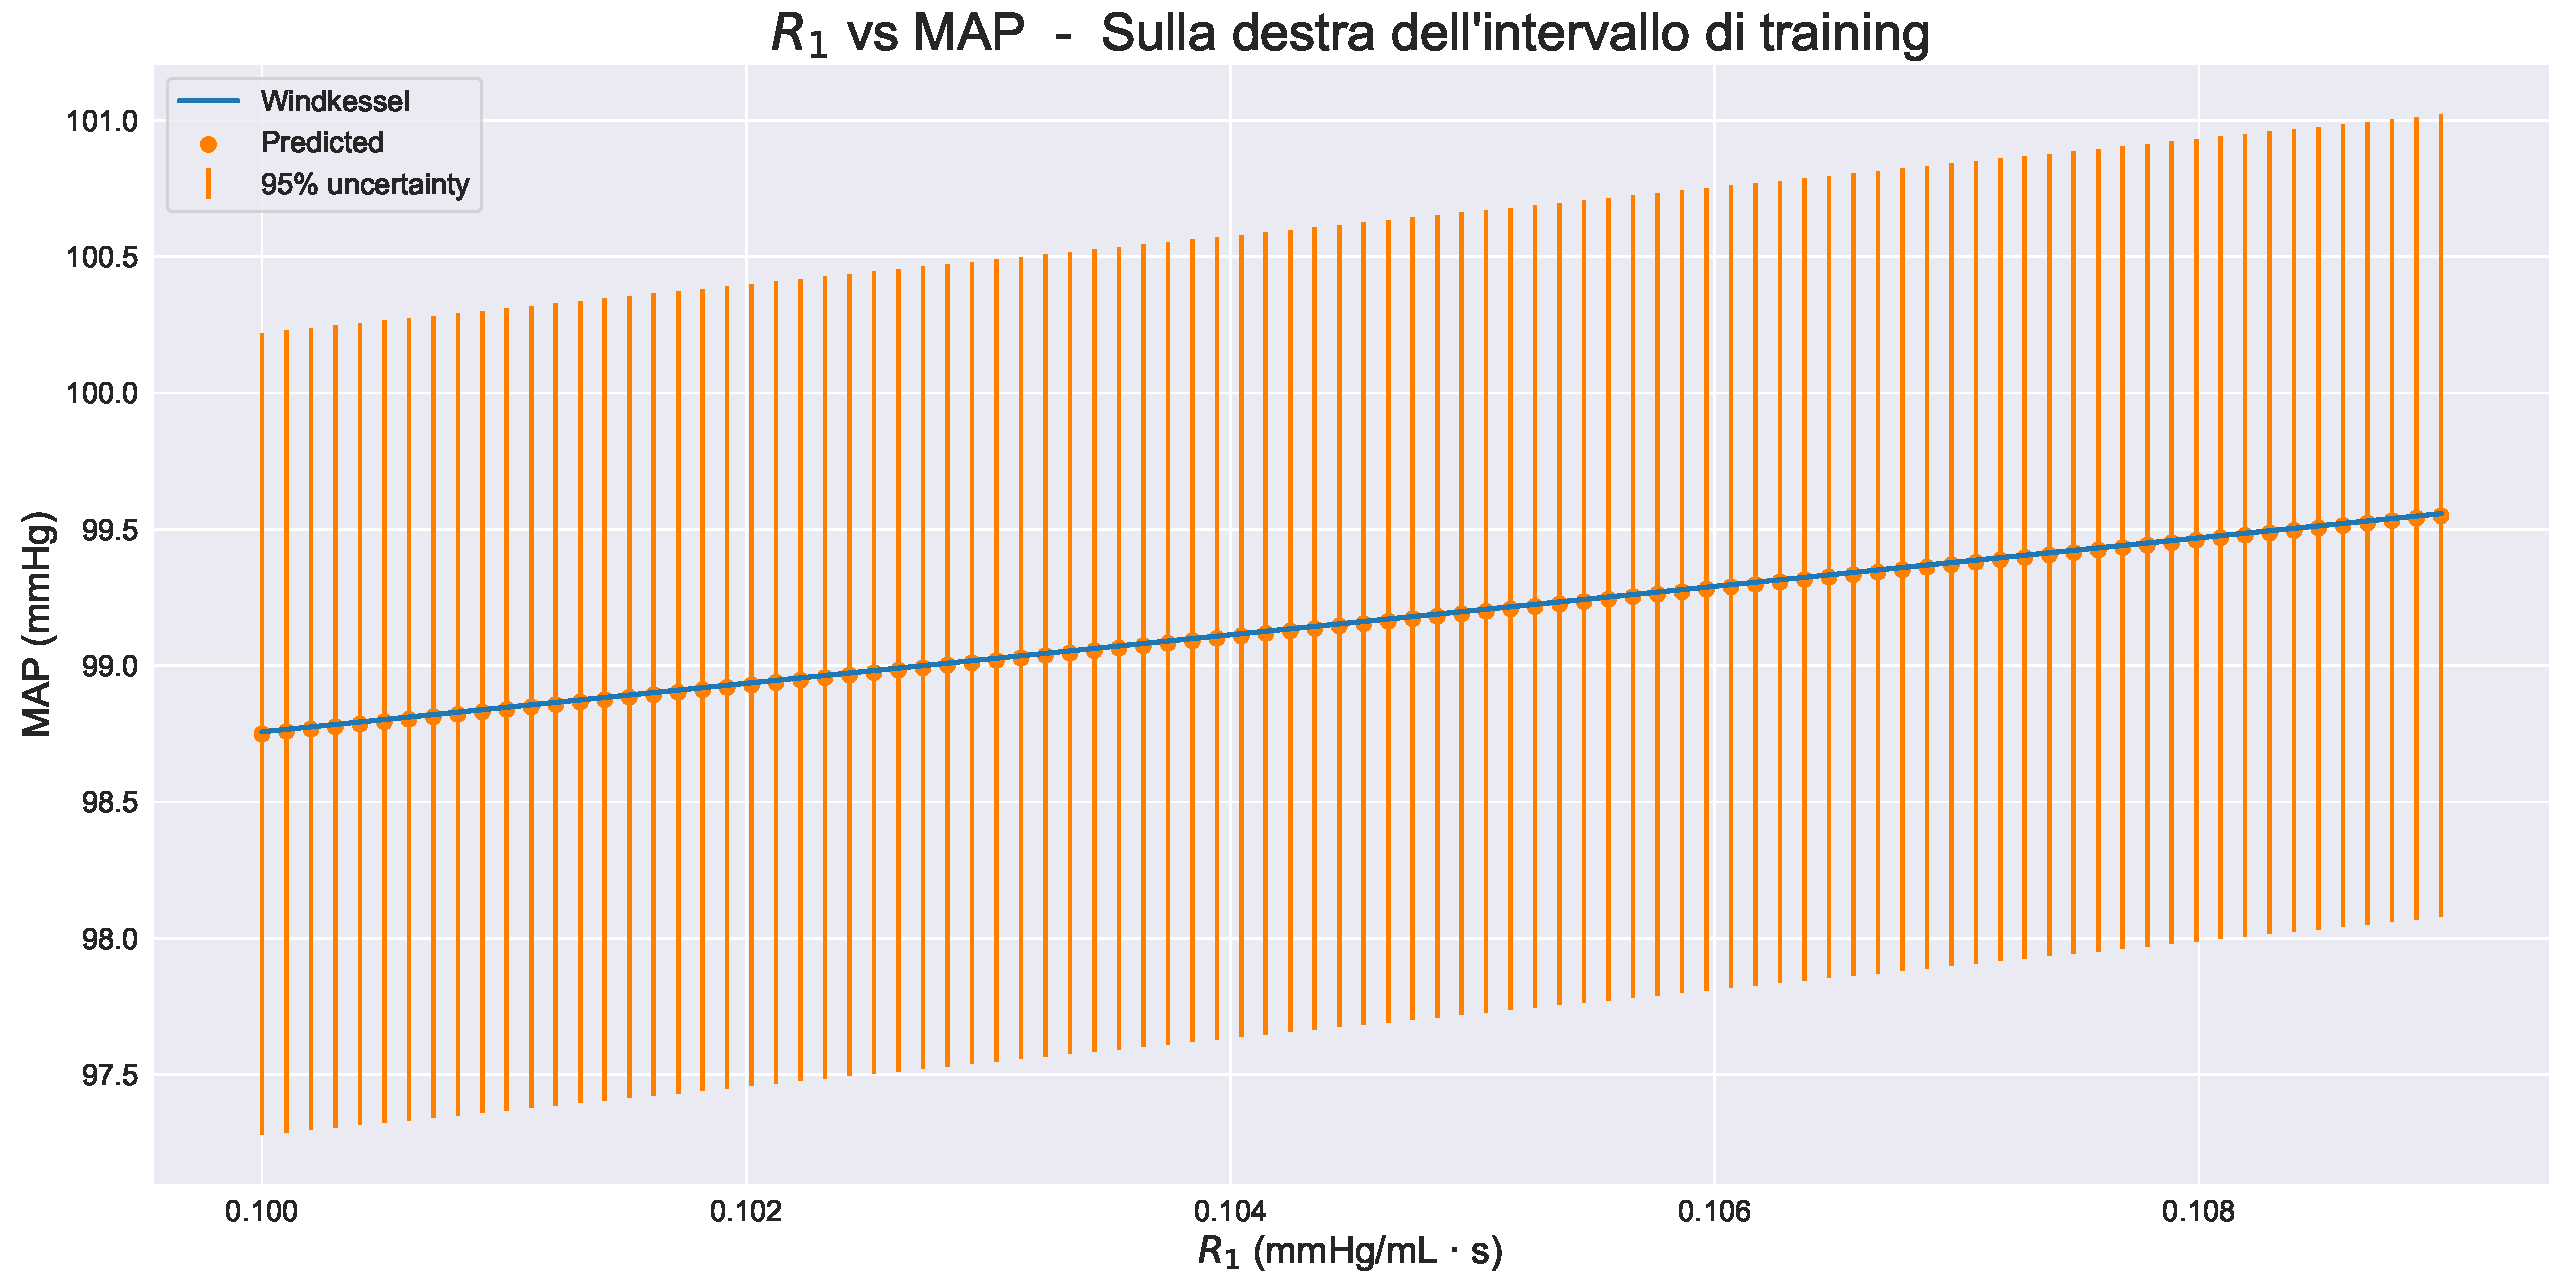
\includegraphics[width=1\textwidth]{images/Training (risultati)/MAP/MAP - R1 - dx.pdf}
    \caption{Dipendenza di MAP da $R1$ sull'intervallo attiguo a destra dell'intervallo di training.}
    \label{MAP - R1 - dx}
\end{figure}




\newpage
% **********
% MAP - R2
% **********
\subsubsection{Dipendenza da $R_2$}
Per studiare la dipendenza da $R_2$ viene usato lo stesso approccio. Il risultato complessivo è mostrato in figura \ref{MAP - R2 - full}, il risultato nel solo intervallo di training in \ref{MAP - R2 - training}, il risultato nei singoli intervalli attigui in \ref{MAP - R2 - sx} e \ref{MAP - R2 - dx}.

\begin{figure}[!htb]
    \centering
    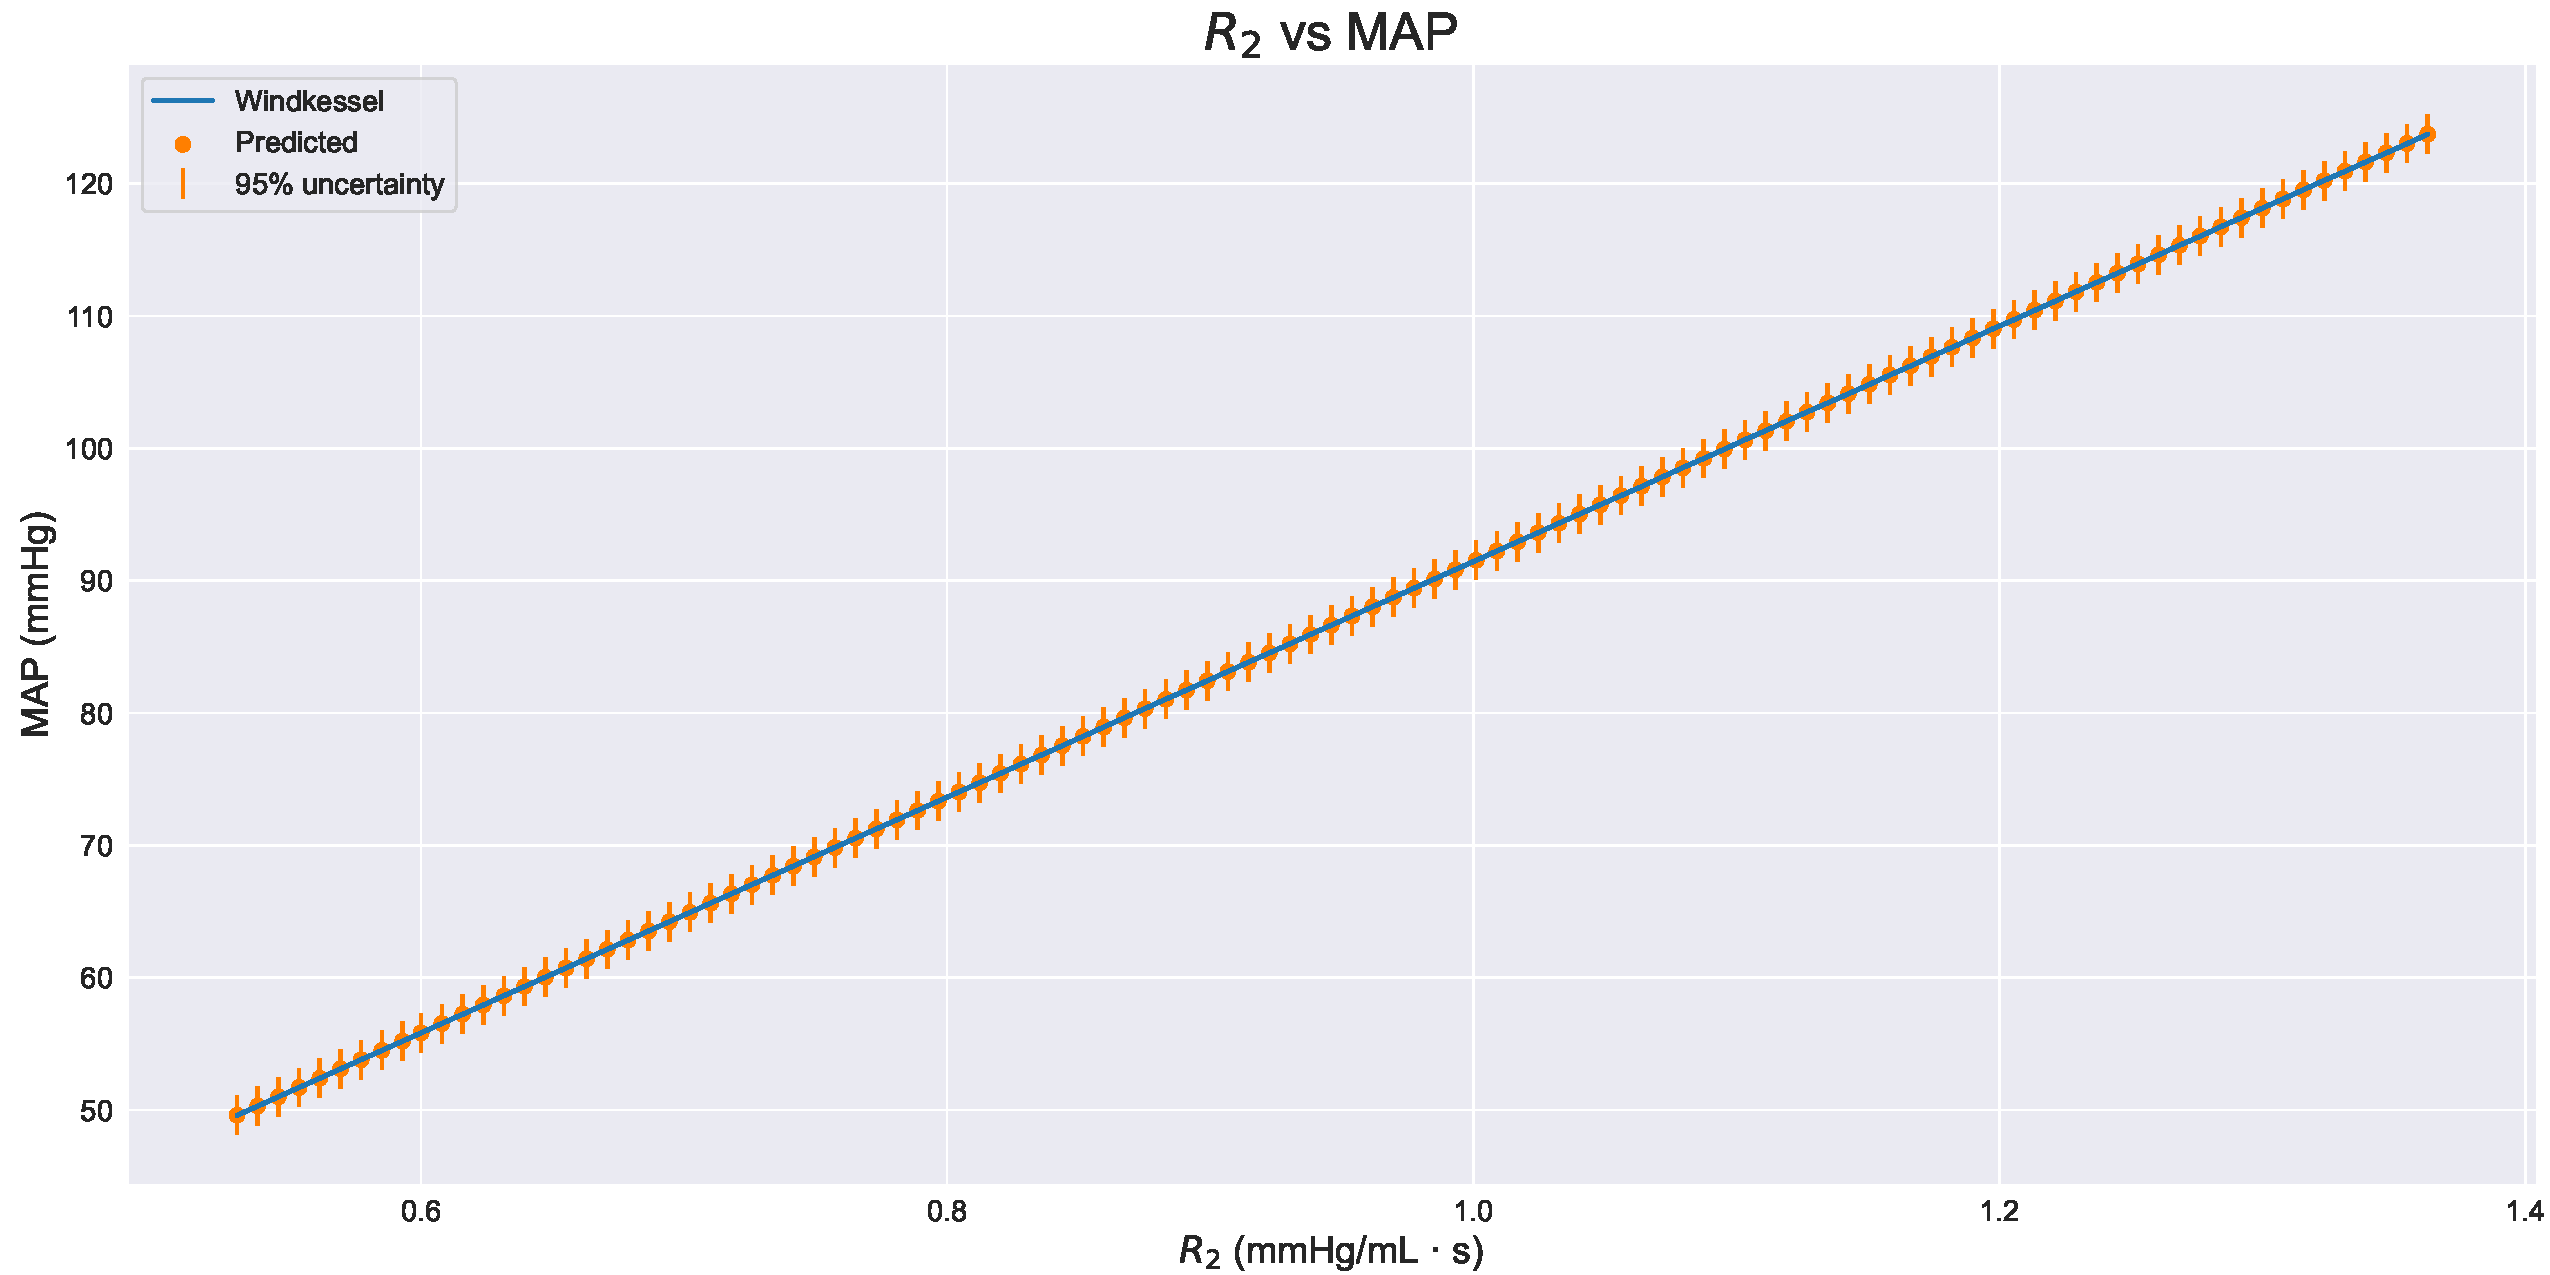
\includegraphics[width=1\textwidth]{images/Training (risultati)/MAP/MAP - R2 - full.pdf}
    \caption{Dipendenza di MAP da $R2$ sull'intervallo di training e due intervalli attigui.}
    \label{MAP - R2 - full}
\end{figure}

\vspace{1cm}

\begin{figure}[!htb]
    \centering
    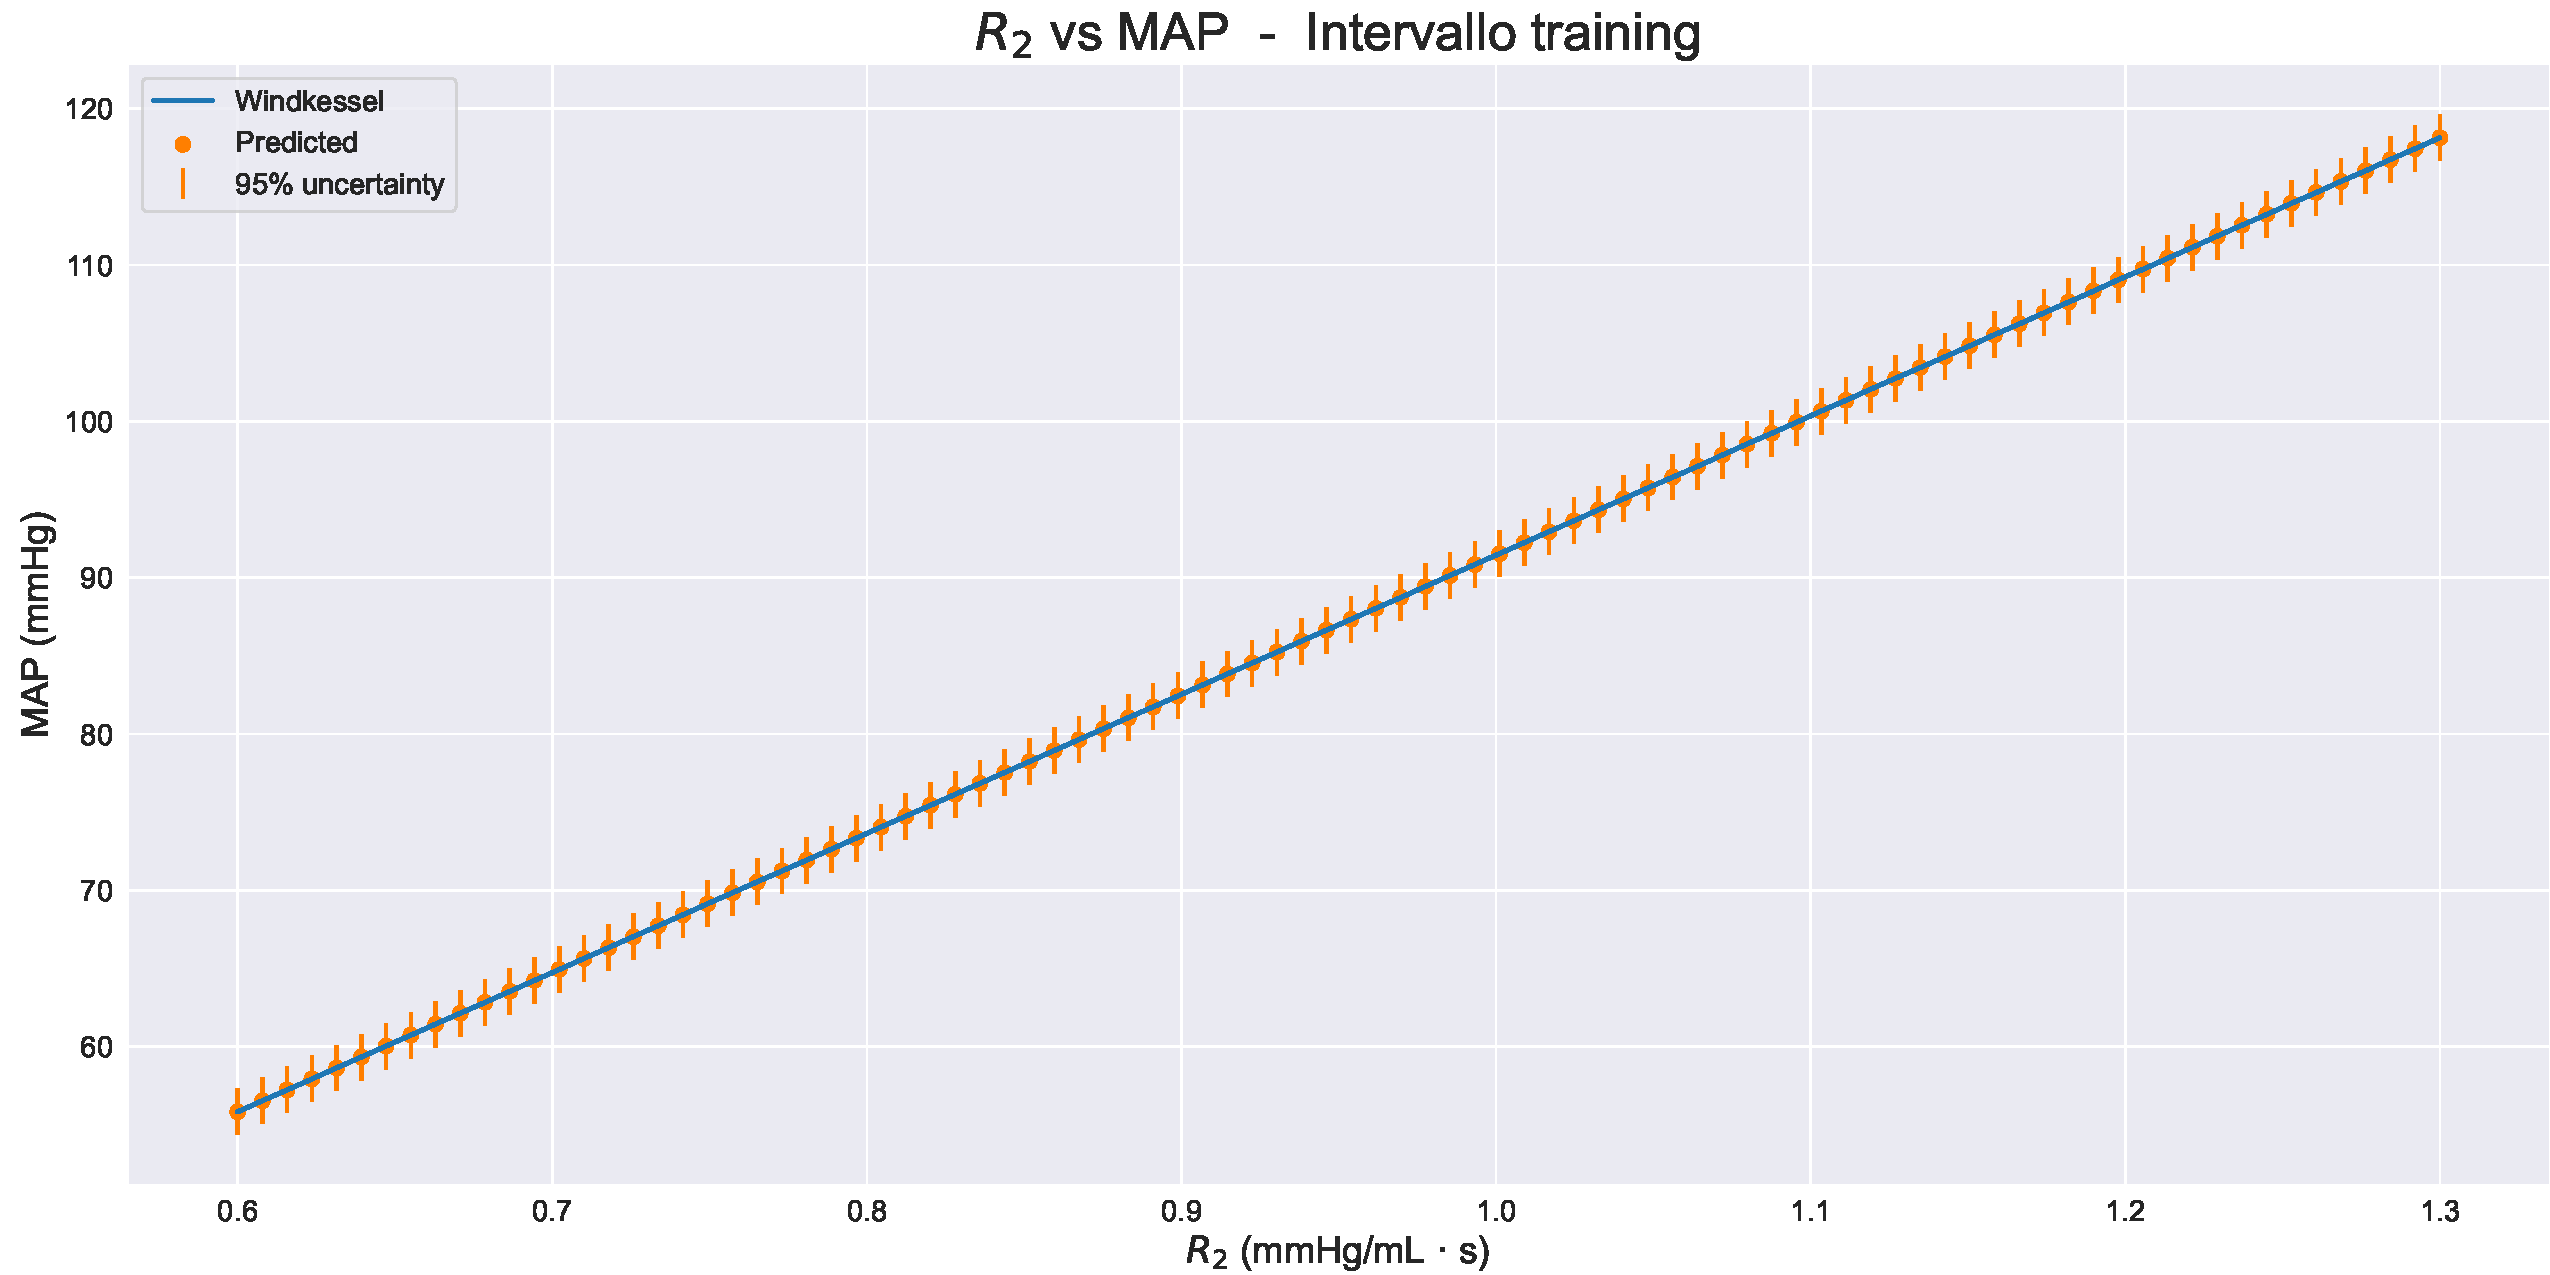
\includegraphics[width=1\textwidth]{images/Training (risultati)/MAP/MAP - R2 - training.pdf}
    \caption{Dipendenza di MAP da $R2$ sull'intervallo di training.}
    \label{MAP - R2 - training}
\end{figure}

\begin{figure}
    \centering
    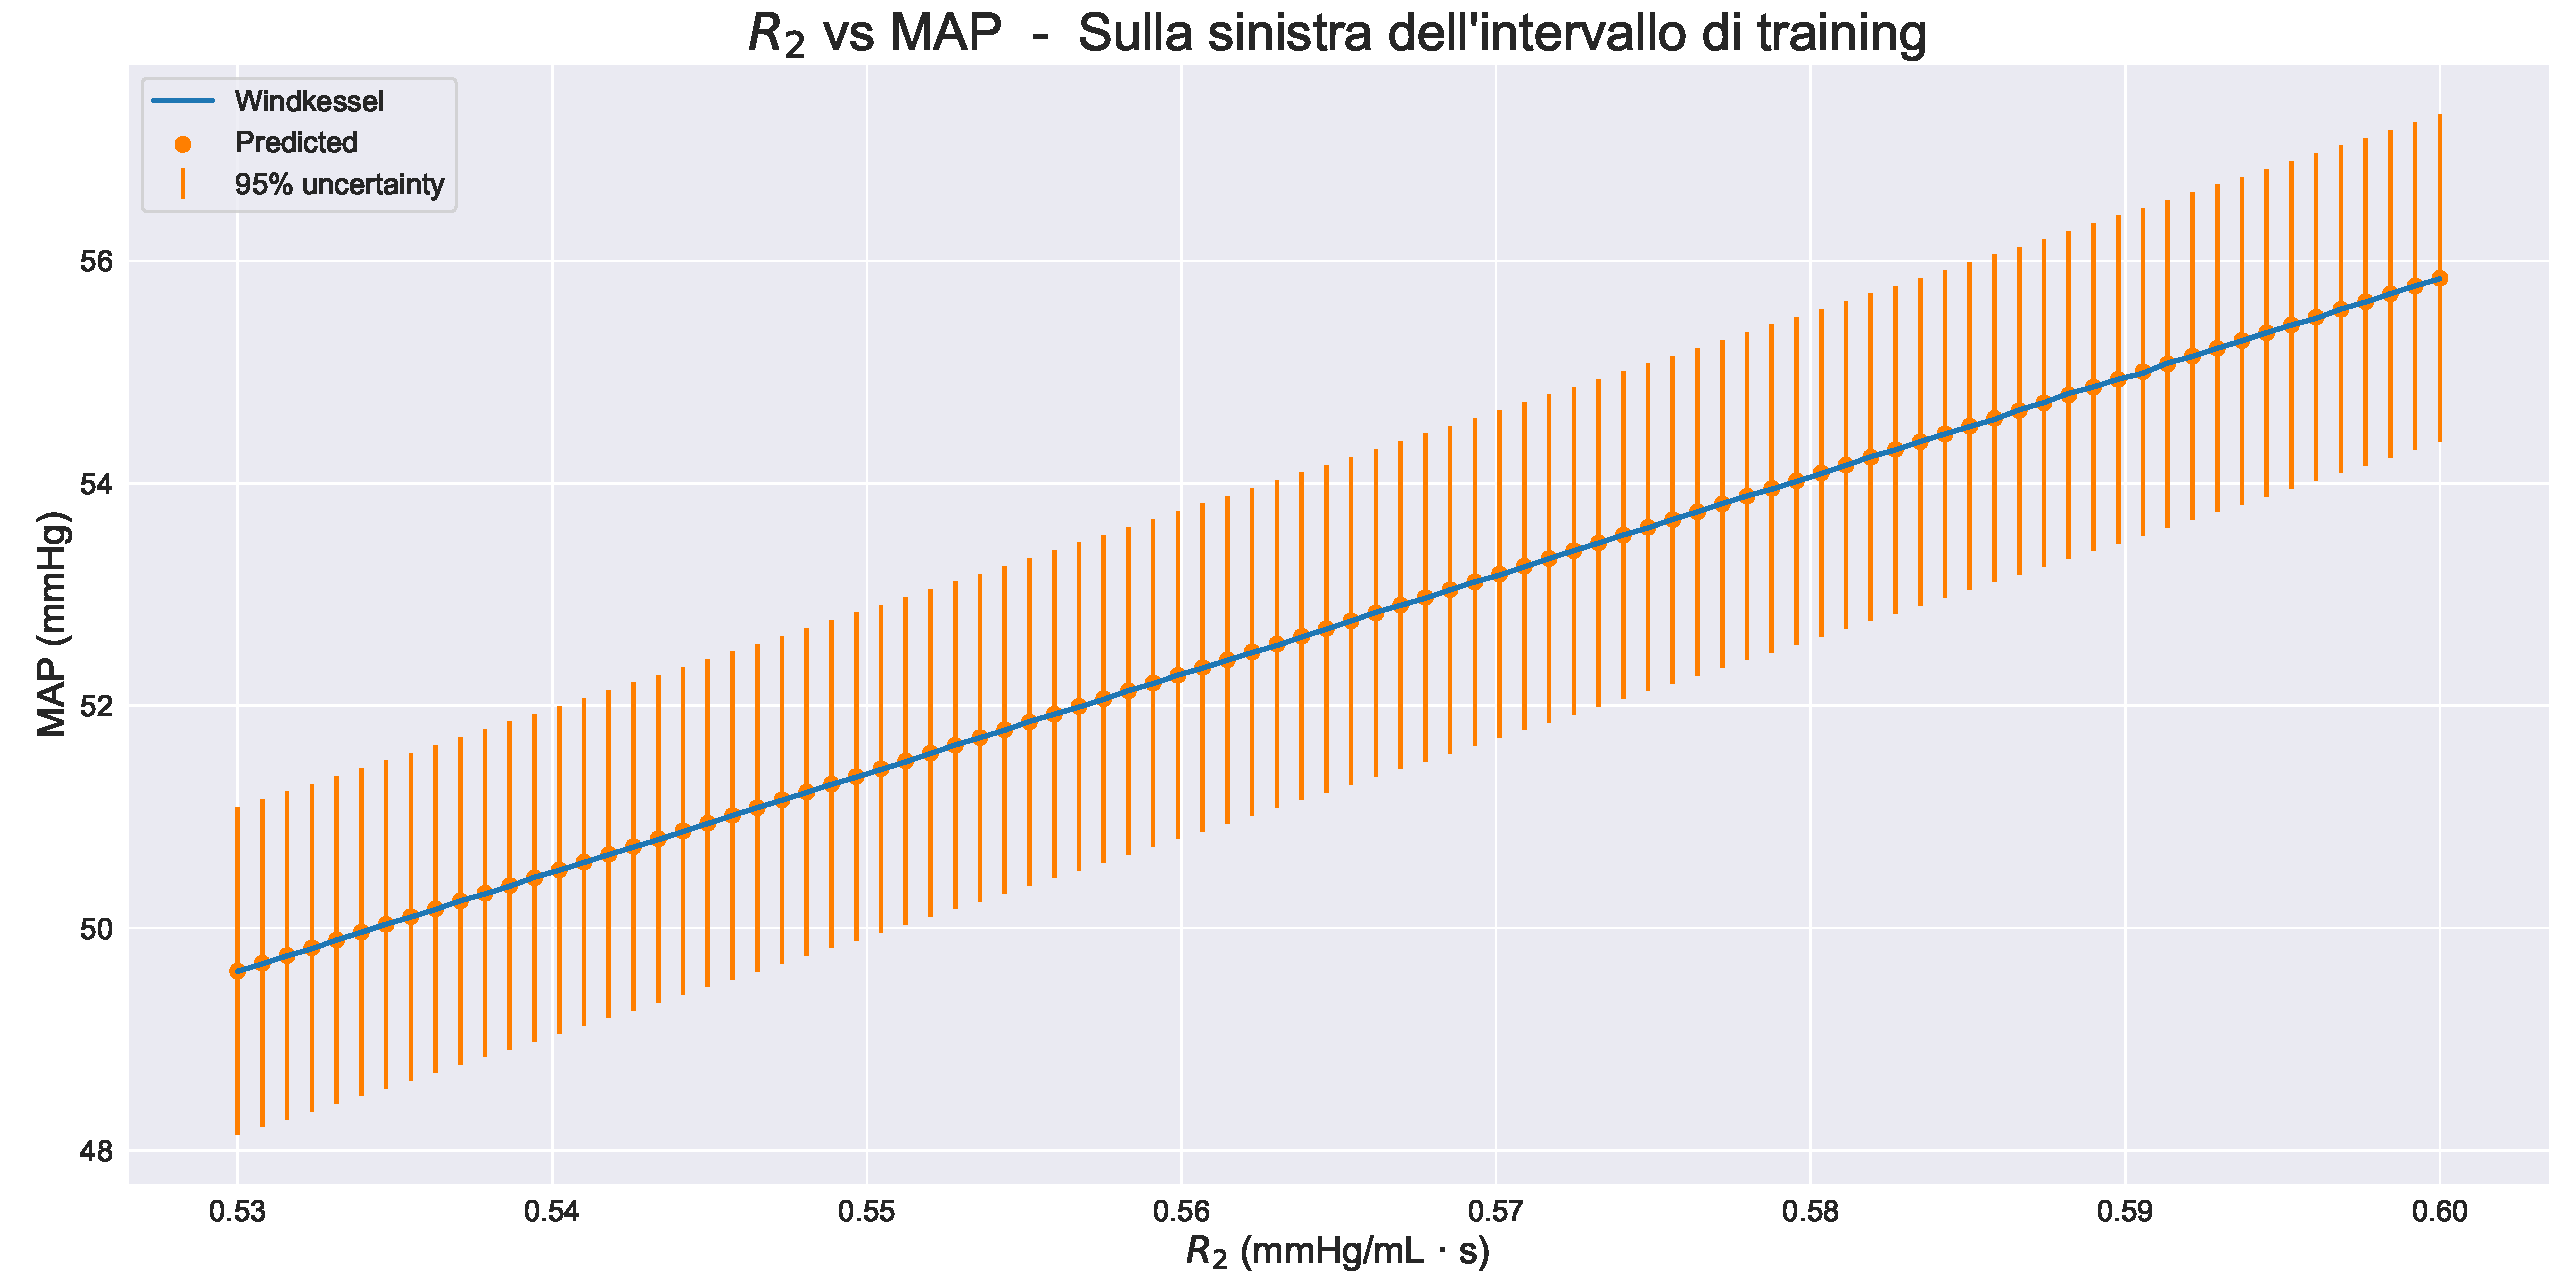
\includegraphics[width=1\textwidth]{images/Training (risultati)/MAP/MAP - R2 - sx.pdf}
    \caption{Dipendenza di MAP da $R2$ sull'intervallo attiguo a sinistra dell'intervallo di training.}
    \label{MAP - R2 - sx}
\end{figure}


\begin{figure}
    \centering
    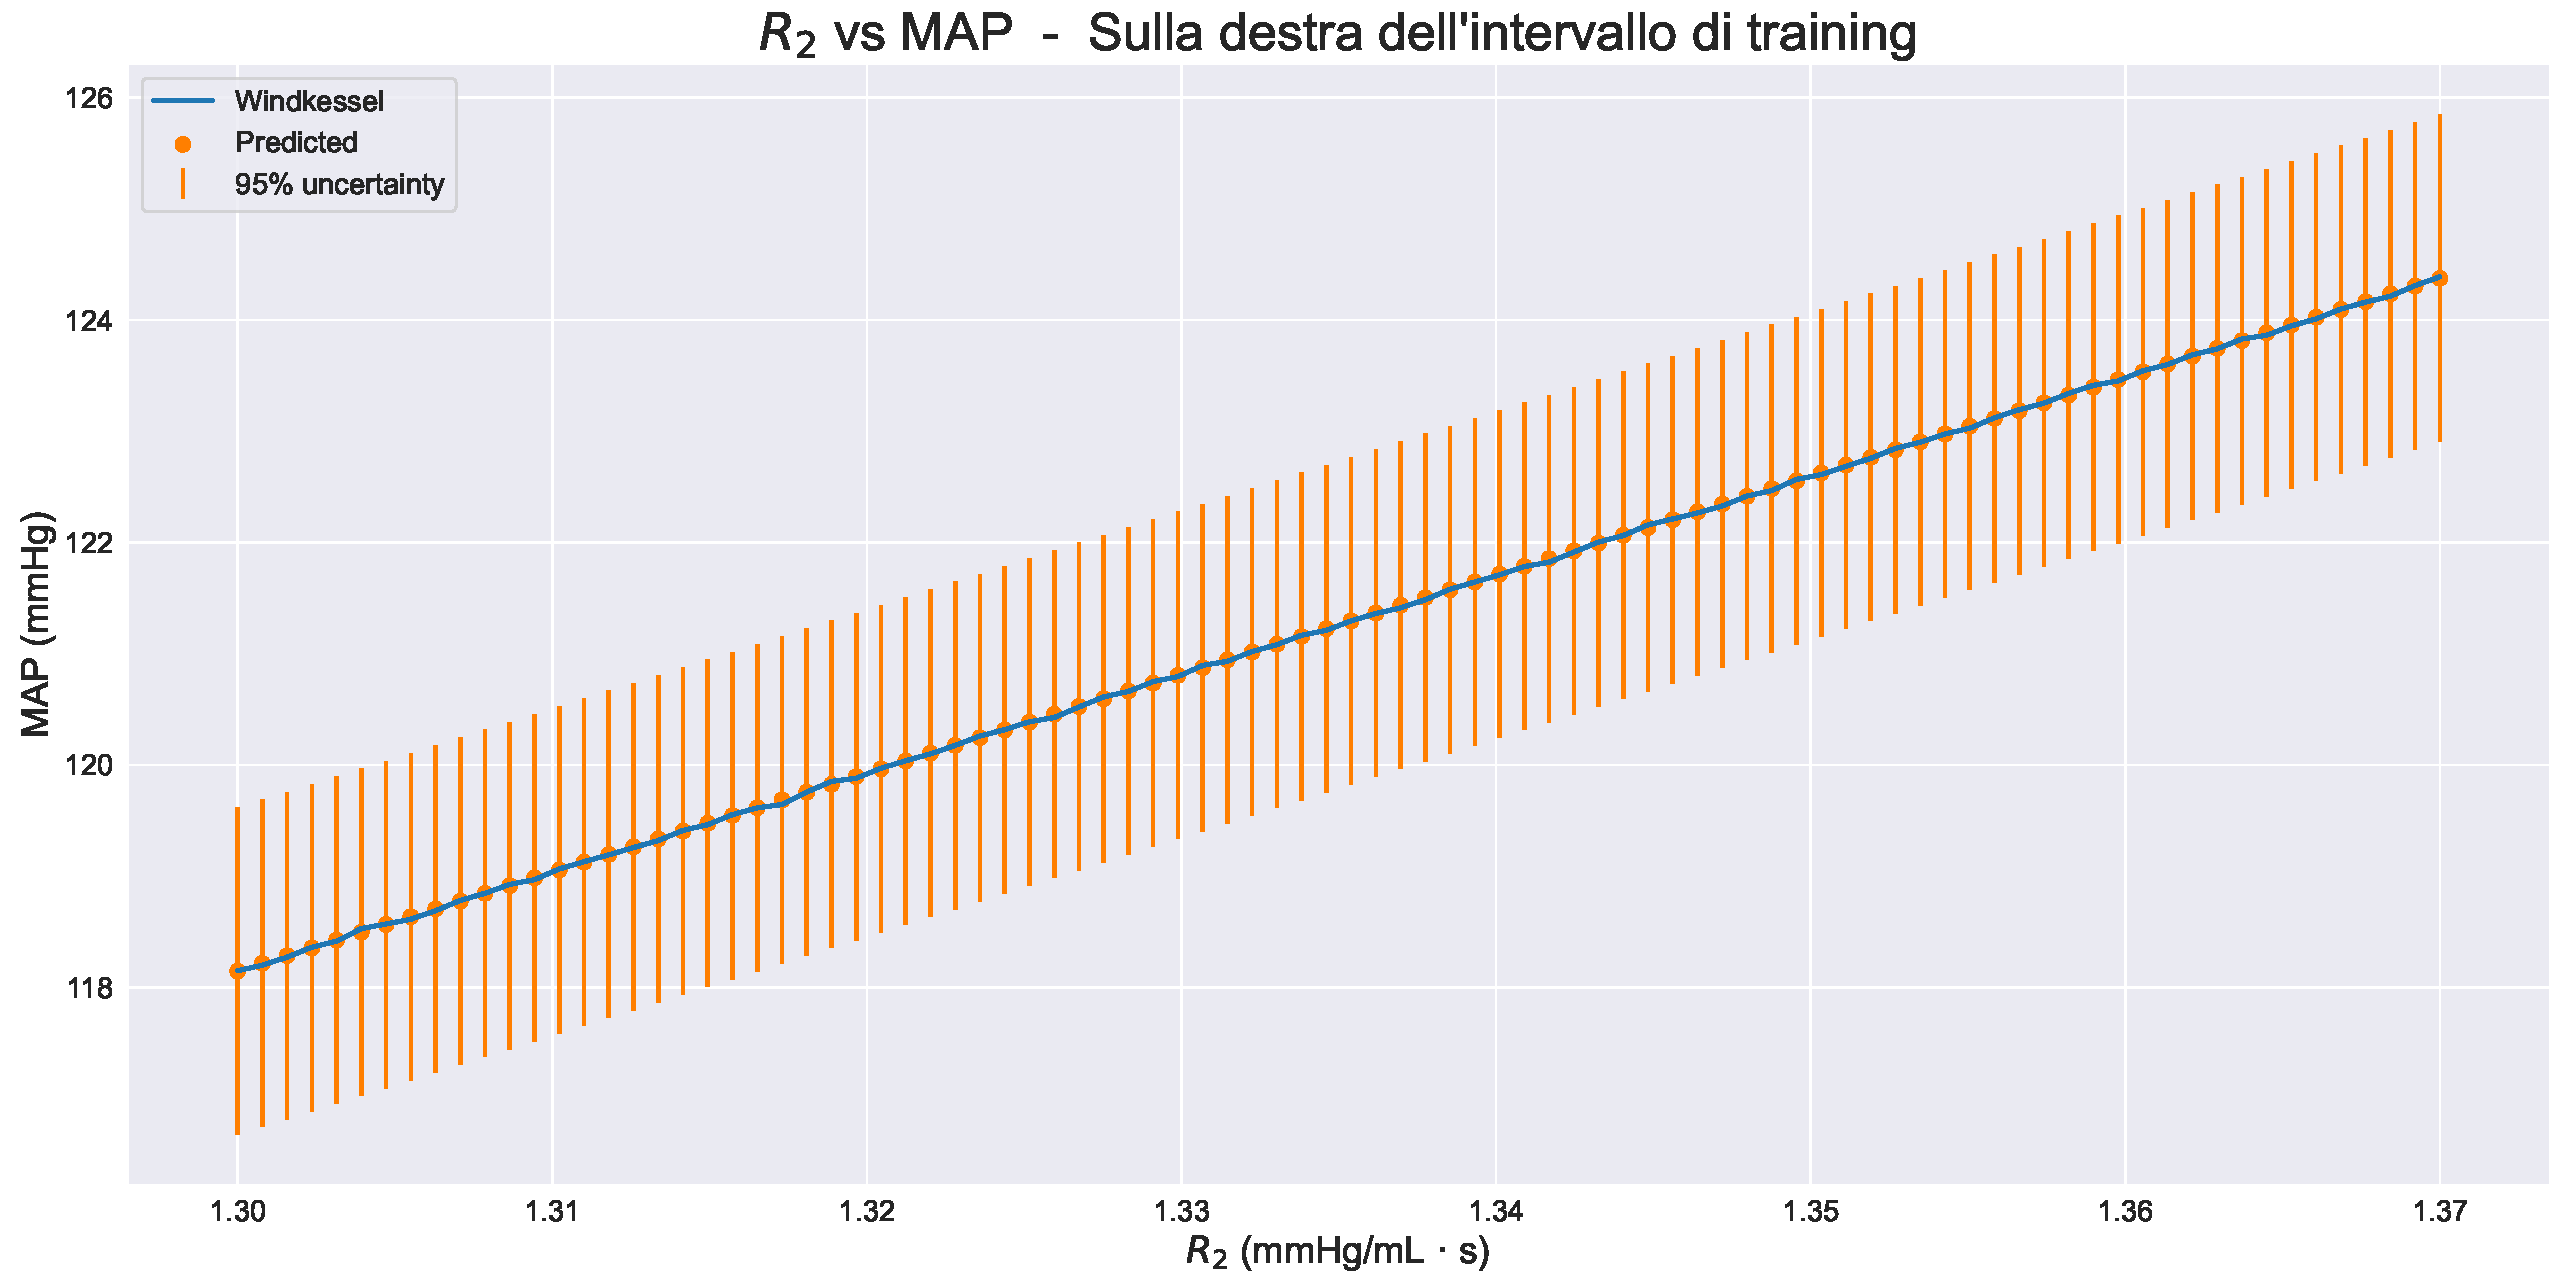
\includegraphics[width=1\textwidth]{images/Training (risultati)/MAP/MAP - R2 - dx.pdf}
    \caption{Dipendenza di MAP da $R2$ sull'intervallo attiguo a destra dell'intervallo di training.}
    \label{MAP - R2 - dx}
\end{figure}







\newpage
%******************************
%*********** DBP **************
%******************************
\subsection{Diastolic blood pressure (DBP)}
Viene imposto $\text{lr}=0.07$ e viene usato l'early stopper \textit{GLEarlyStoppingCriterion} con parametri: $\alpha = 2$, $\text{patience}=2$.



% **********
% DBP - loss
% **********
\subsubsection{Training e validation loss}
Il training ha necessitato centotrentuno EPOCHS, ha concluso con $\text{R2Score}=0.9999$, $\text{MeanSquaredError}=0.0001$. In figura \ref{DBP - loss} viene mostrato l'andamento del training e validation loss con MSE e R2Score; in verde l'andamento dell'early stopper.
\begin{figure}[h]
    \centering
    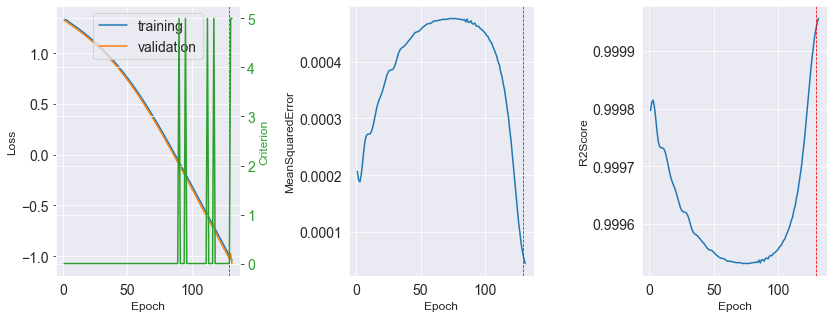
\includegraphics[width=1\textwidth]{images/Training (risultati)/DBP/DBP - loss.png}
    \caption{DBP: andamento del training e validation loss, early stopper, R2Score e MSE.}
    \label{DBP - loss}
\end{figure}

\vspace{-0.5cm}

% **********
% DBP - inference
% **********
\subsubsection{Approssimazione dei dati di input}
In figura \ref{DBP - inference} viene mostrato come le predizioni approssimano i dati di input. La lunghezza delle barre di errore è $0.0028$.

\begin{figure}[h]
    \centering
    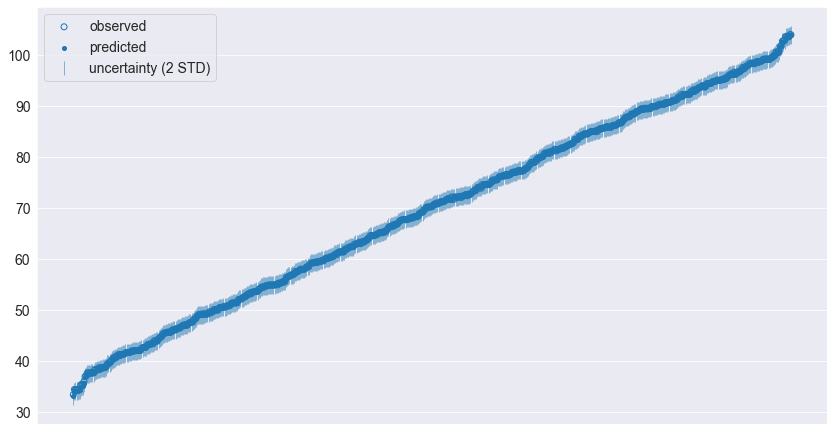
\includegraphics[width=1\textwidth]{images/Training (risultati)/DBP/DBP - inference.png}
    \caption{DBP: predizioni sui dati di input.}
    \label{DBP - inference}
\end{figure}



% **********
% DBP - C
% **********
\subsubsection{Dipendenza da $C$}
Il risultato complessivo è mostrato in figura \ref{DBP - C - full}, il risultato nel solo intervallo di training in \ref{DBP - C - training}, il risultato nei singoli intervalli attigui in \ref{DBP - C - sx} e \ref{DBP - C - dx}. In tutti gli intervalli il modello riesce a generare ottime predizioni con una bassa incertezza (rappresentata dalle barre di errore).

\vspace{1cm}

\begin{figure}[!htb]
    \centering
    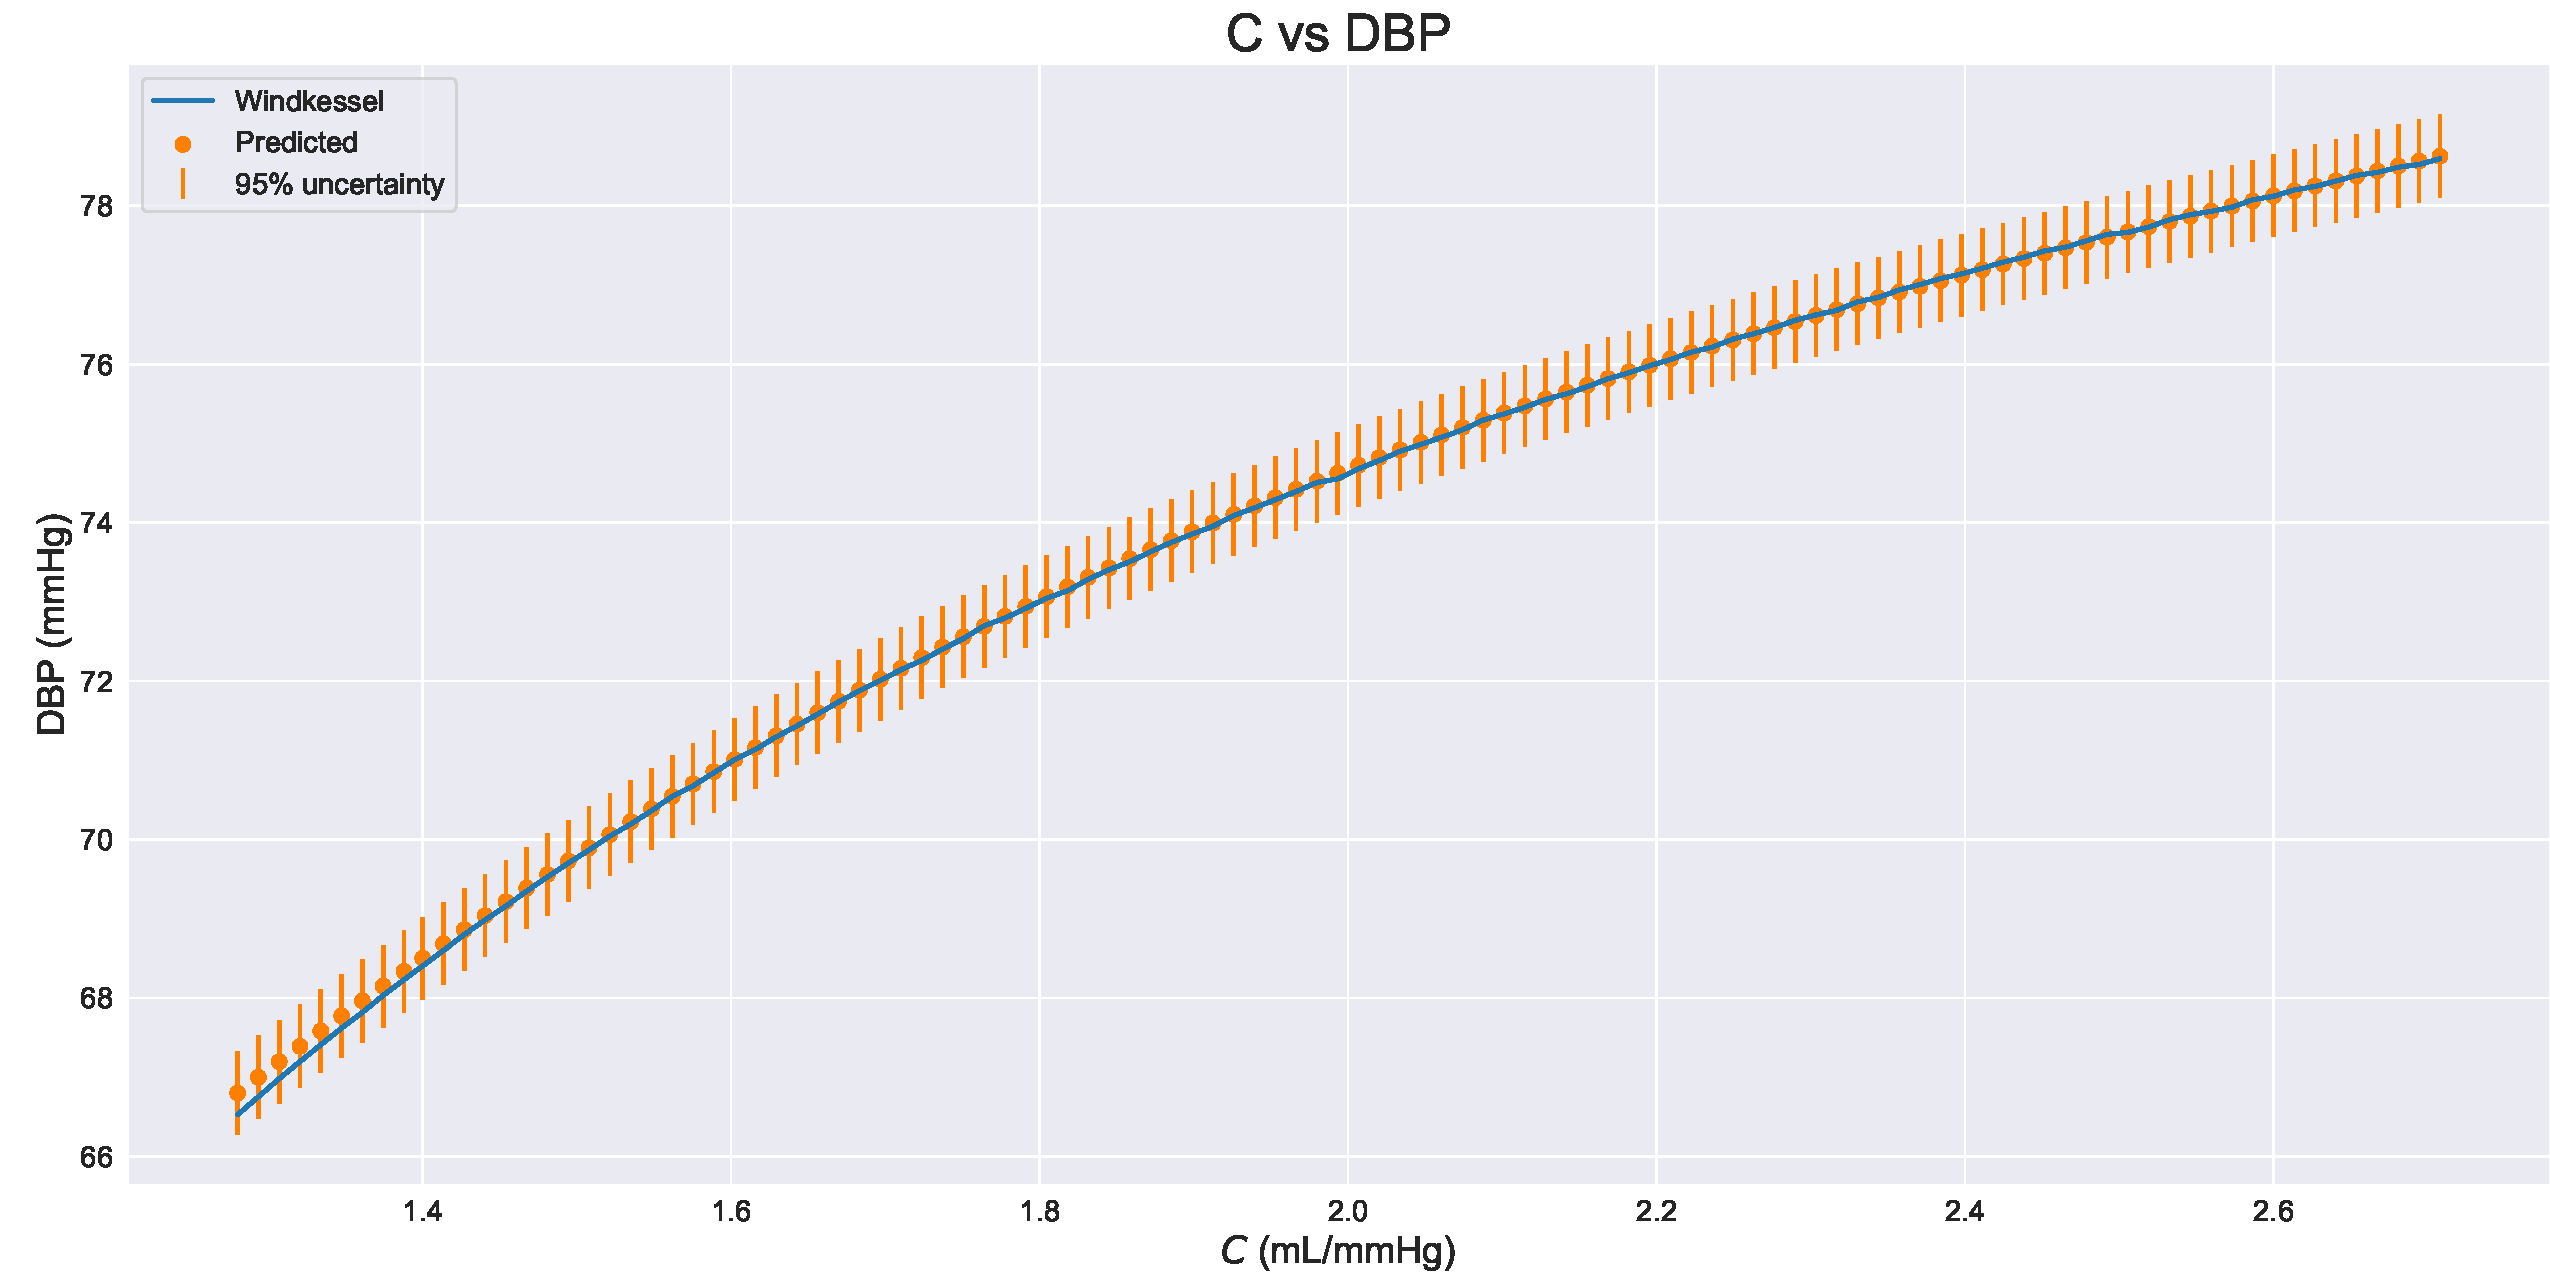
\includegraphics[width=1\textwidth]{images/Training (risultati)/DBP/DBP - C - full.pdf}
    \caption{Dipendenza di DBP da $C$ sull'intervallo di training e due intervalli attigui.}
    \label{DBP - C - full}
\end{figure}

\vspace{0.32cm}

\begin{figure}[!htb]
    \centering
    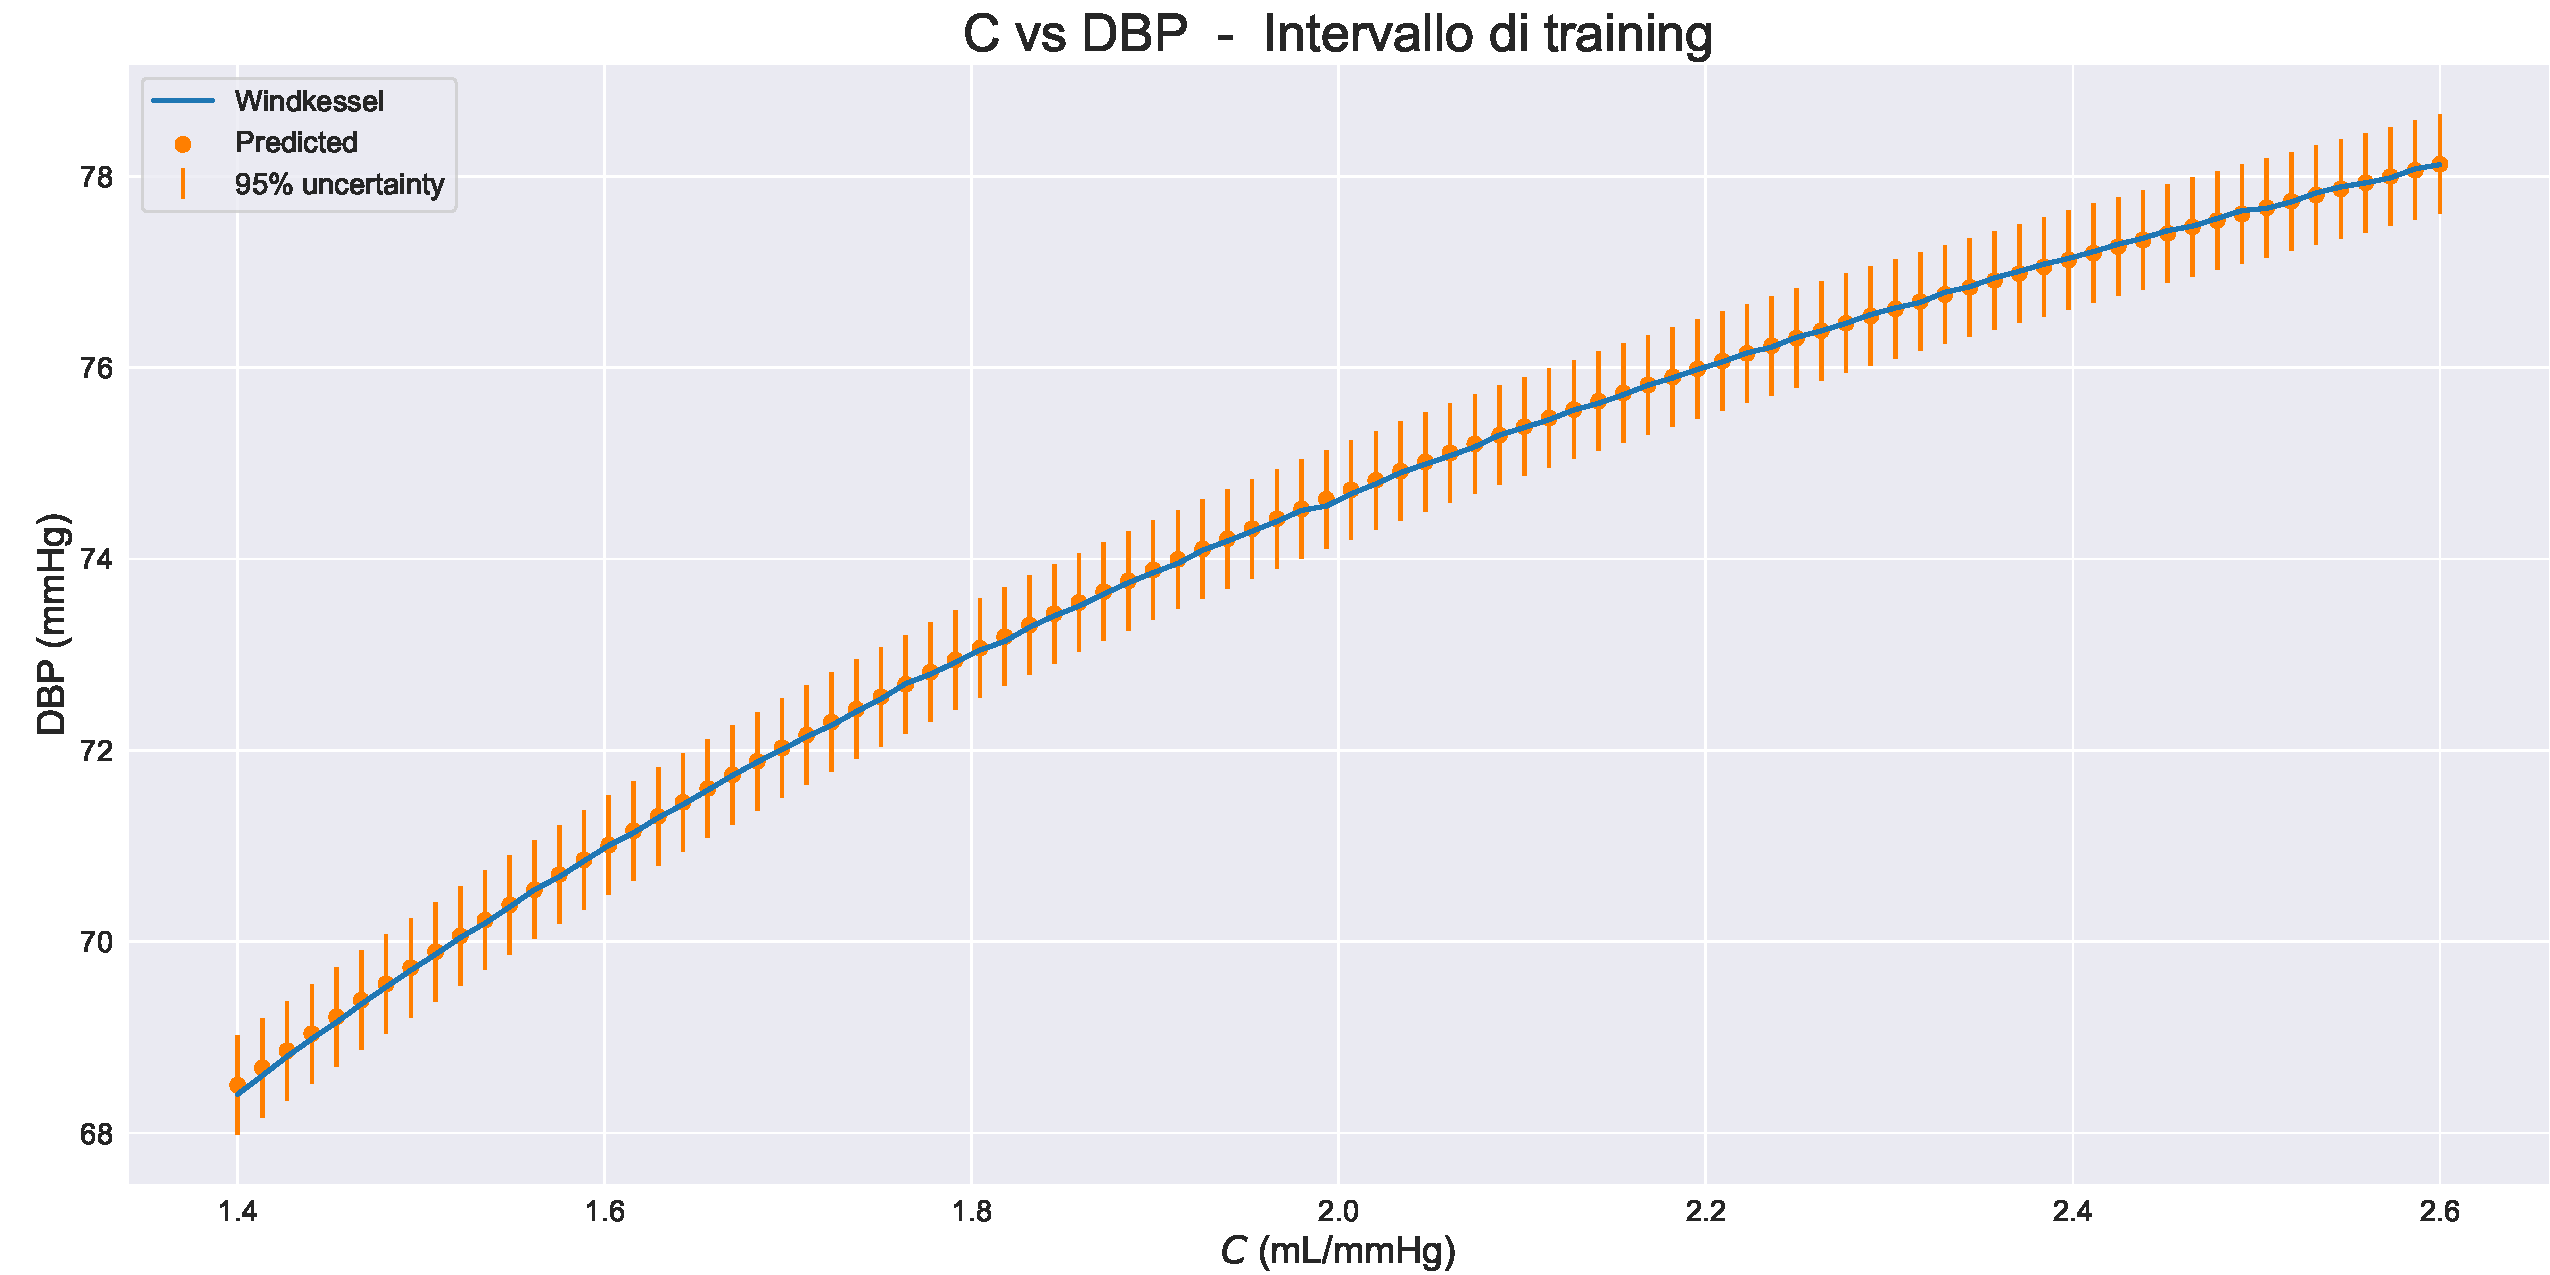
\includegraphics[width=1\textwidth]{images/Training (risultati)/DBP/DBP - C - training.pdf}
    \caption{Dipendenza di DBP da $C$ sull'intervallo di training.}
    \label{DBP - C - training}
\end{figure}



\begin{figure}
    \centering
    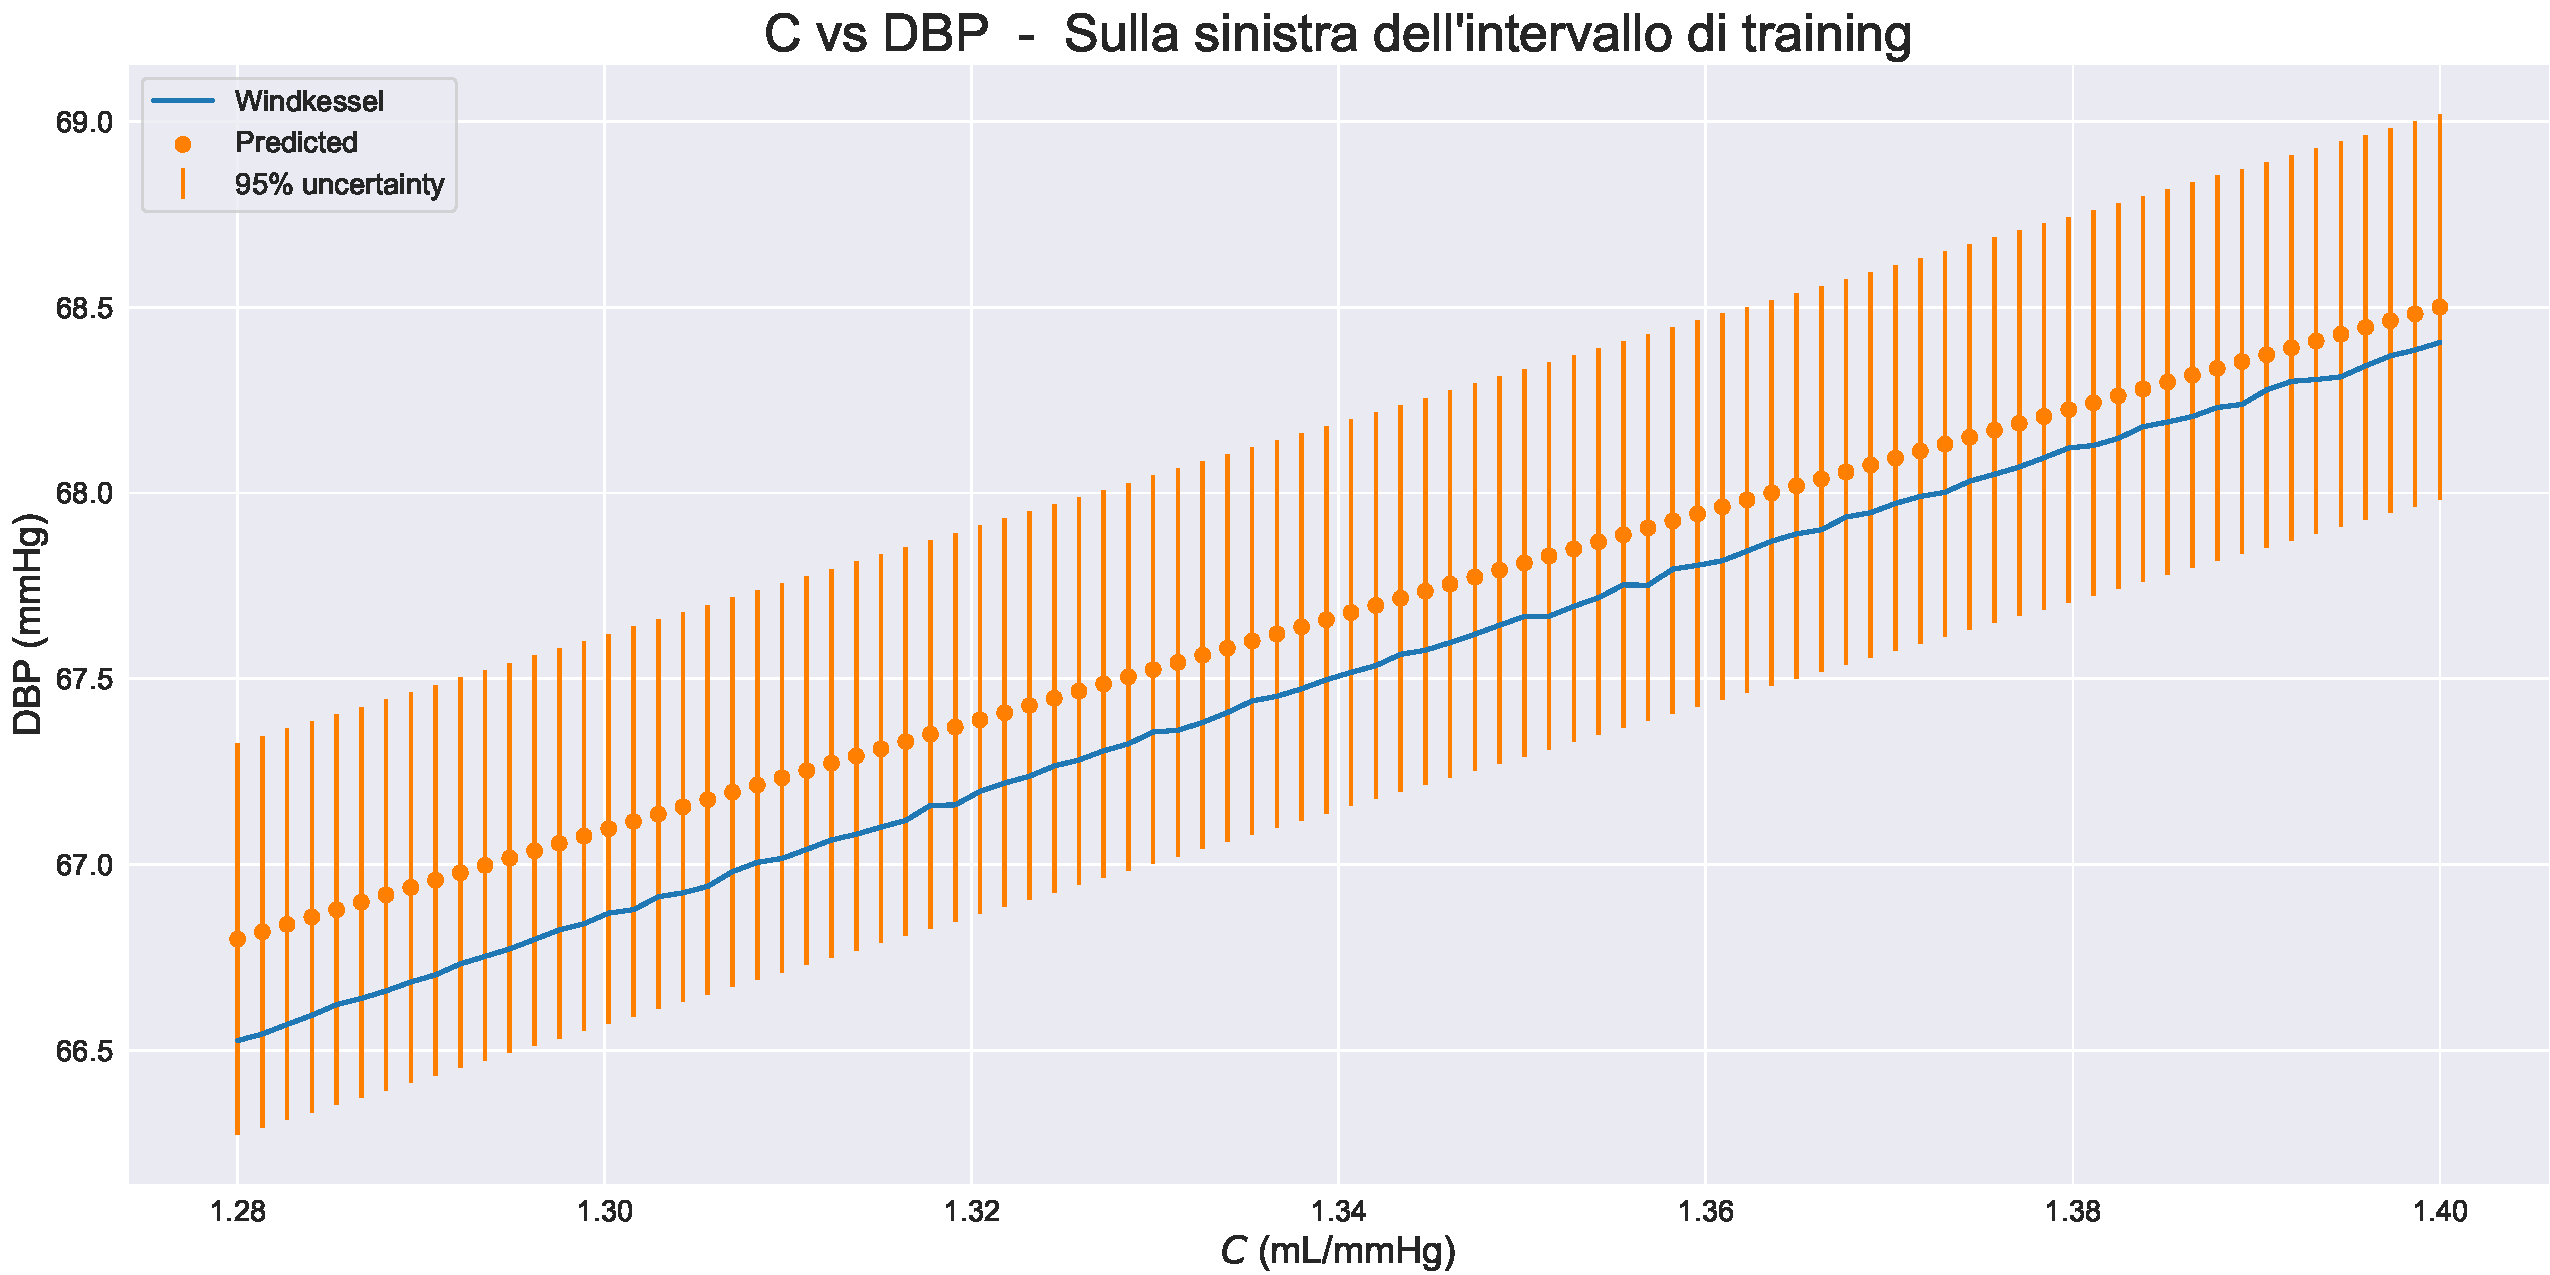
\includegraphics[width=1\textwidth]{images/Training (risultati)/DBP/DBP - C - sx.pdf}
    \caption{Dipendenza di DBP da $C$ sull'intervallo attiguo a sinistra dell'intervallo di training.}
    \label{DBP - C - sx}
\end{figure}


\begin{figure}
    \centering
    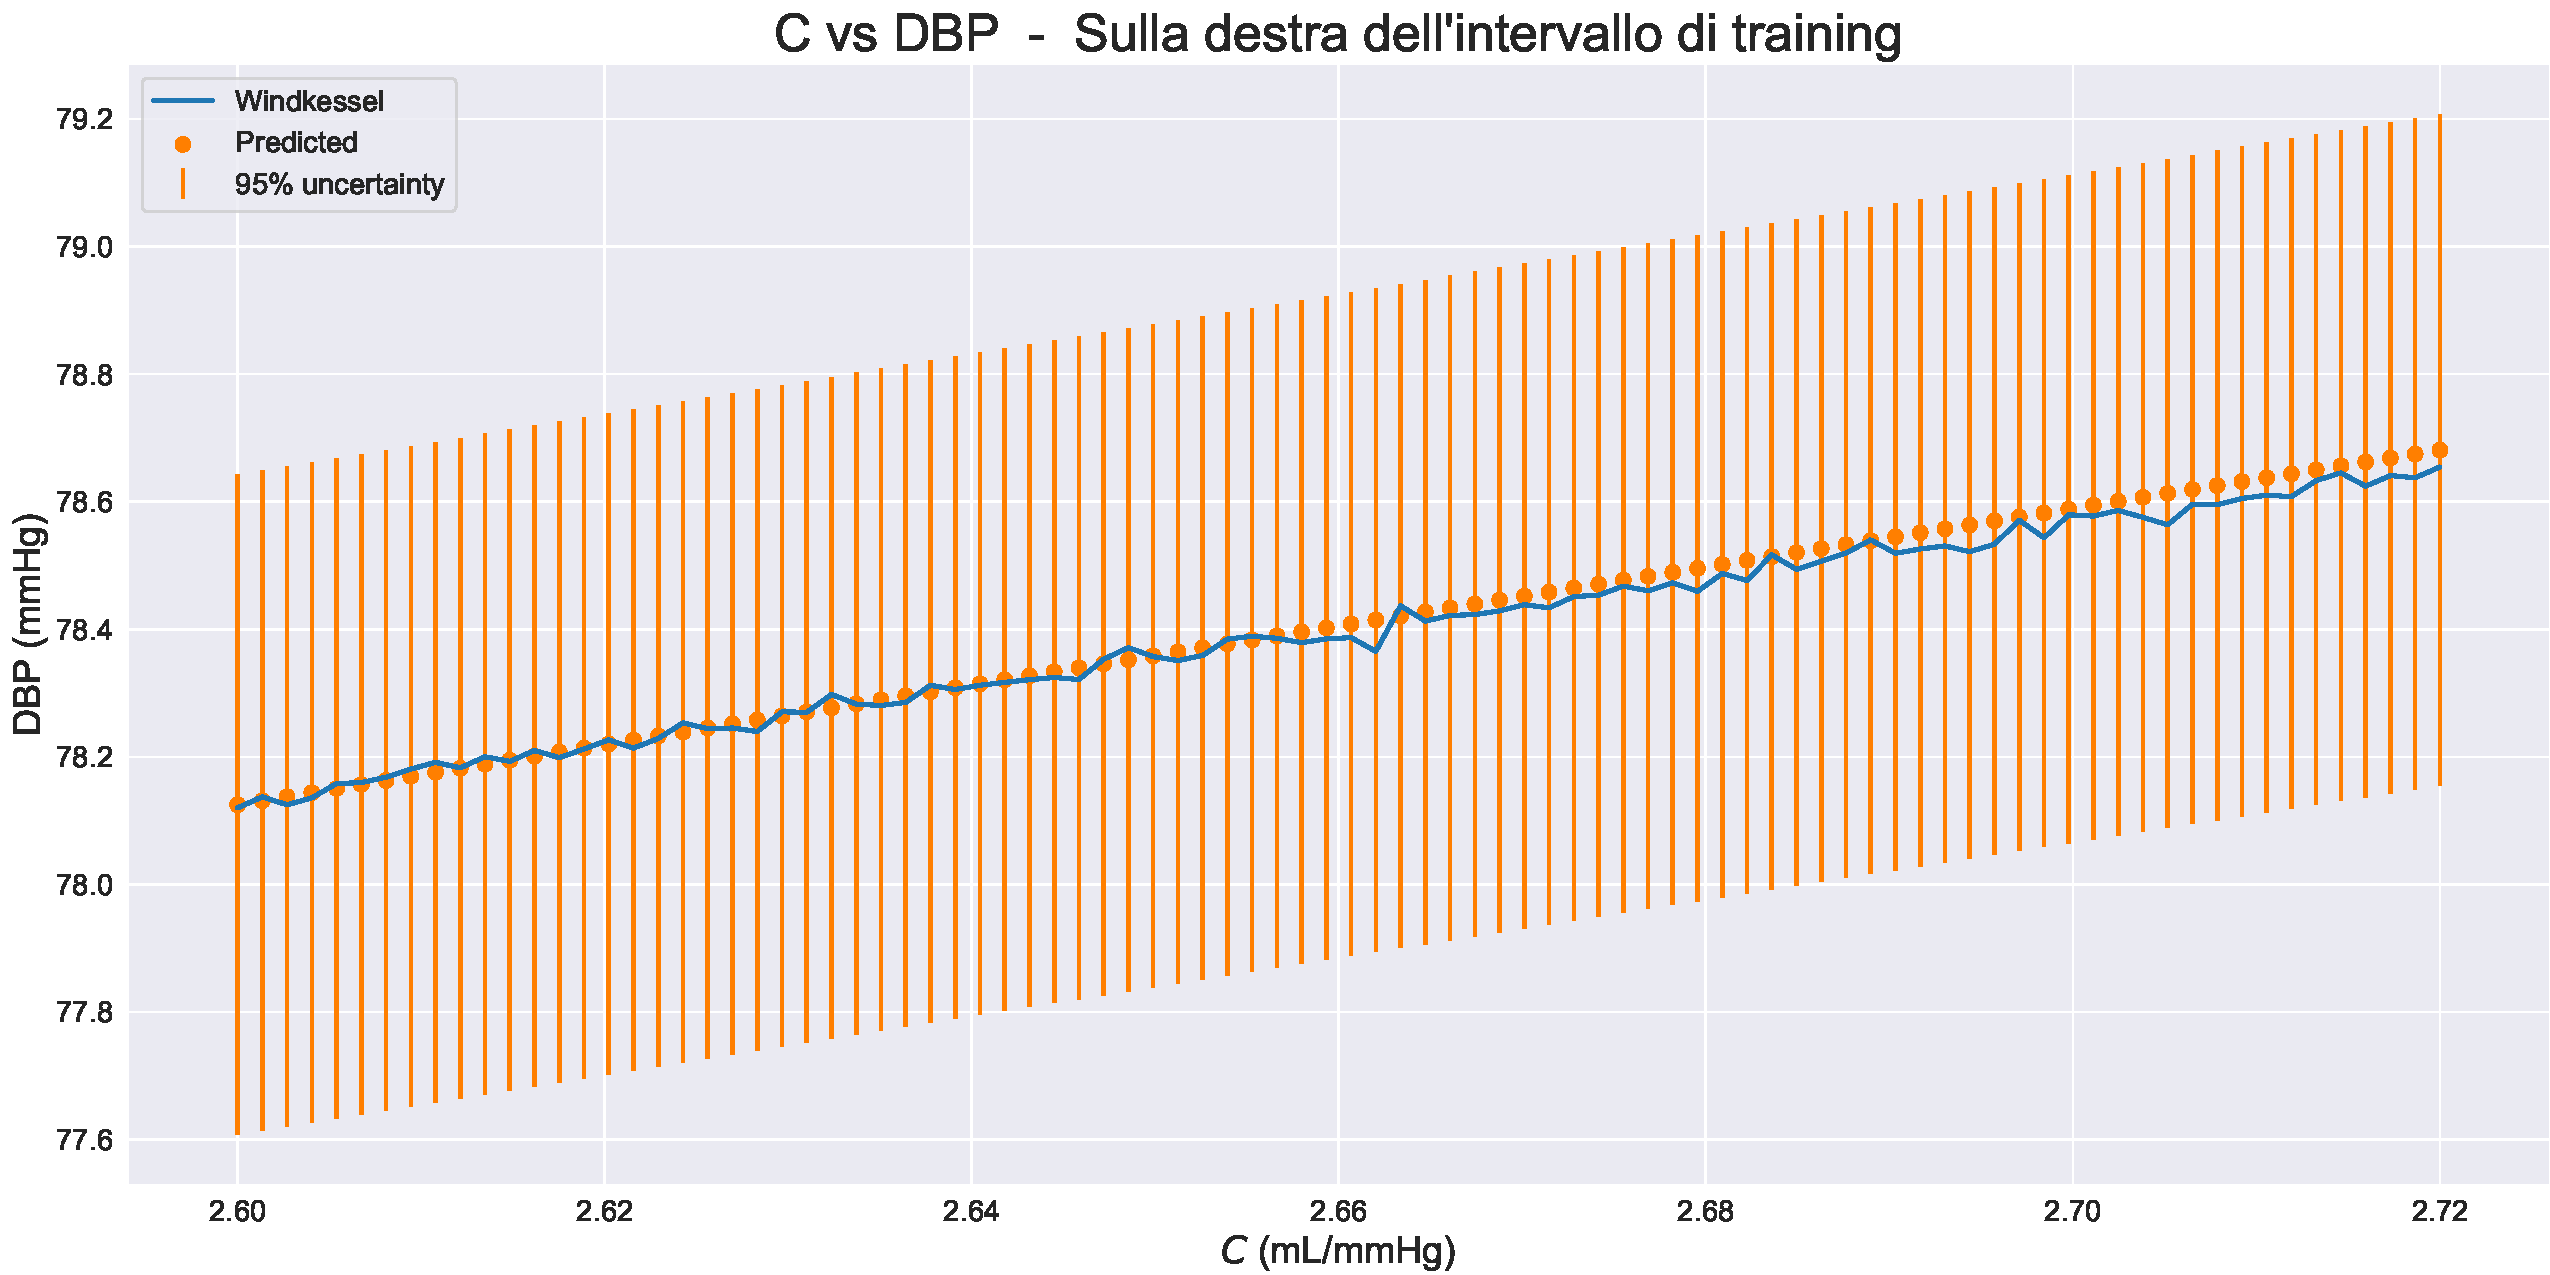
\includegraphics[width=1\textwidth]{images/Training (risultati)/DBP/DBP - C - dx.pdf}
    \caption{Dipendenza di DBP da $C$ sull'intervallo attiguo a destra dell'intervallo di training.}
    \label{DBP - C - dx}
\end{figure}


\newpage

% **********
% DBP - R1
% **********
\subsubsection{Dipendenza da $R_1$}
Il risultato complessivo è mostrato in figura \ref{DBP - R1 - full}, il risultato nel solo intervallo di training in \ref{DBP - R1 - training}, il risultato nei singoli intervalli attigui in \ref{DBP - R1 - sx} e \ref{DBP - R1 - dx}. Anche in questo caso il modello è in grado di fare predizioni molto precise.

\vspace{1cm}

\begin{figure}[!htb]
    \centering
    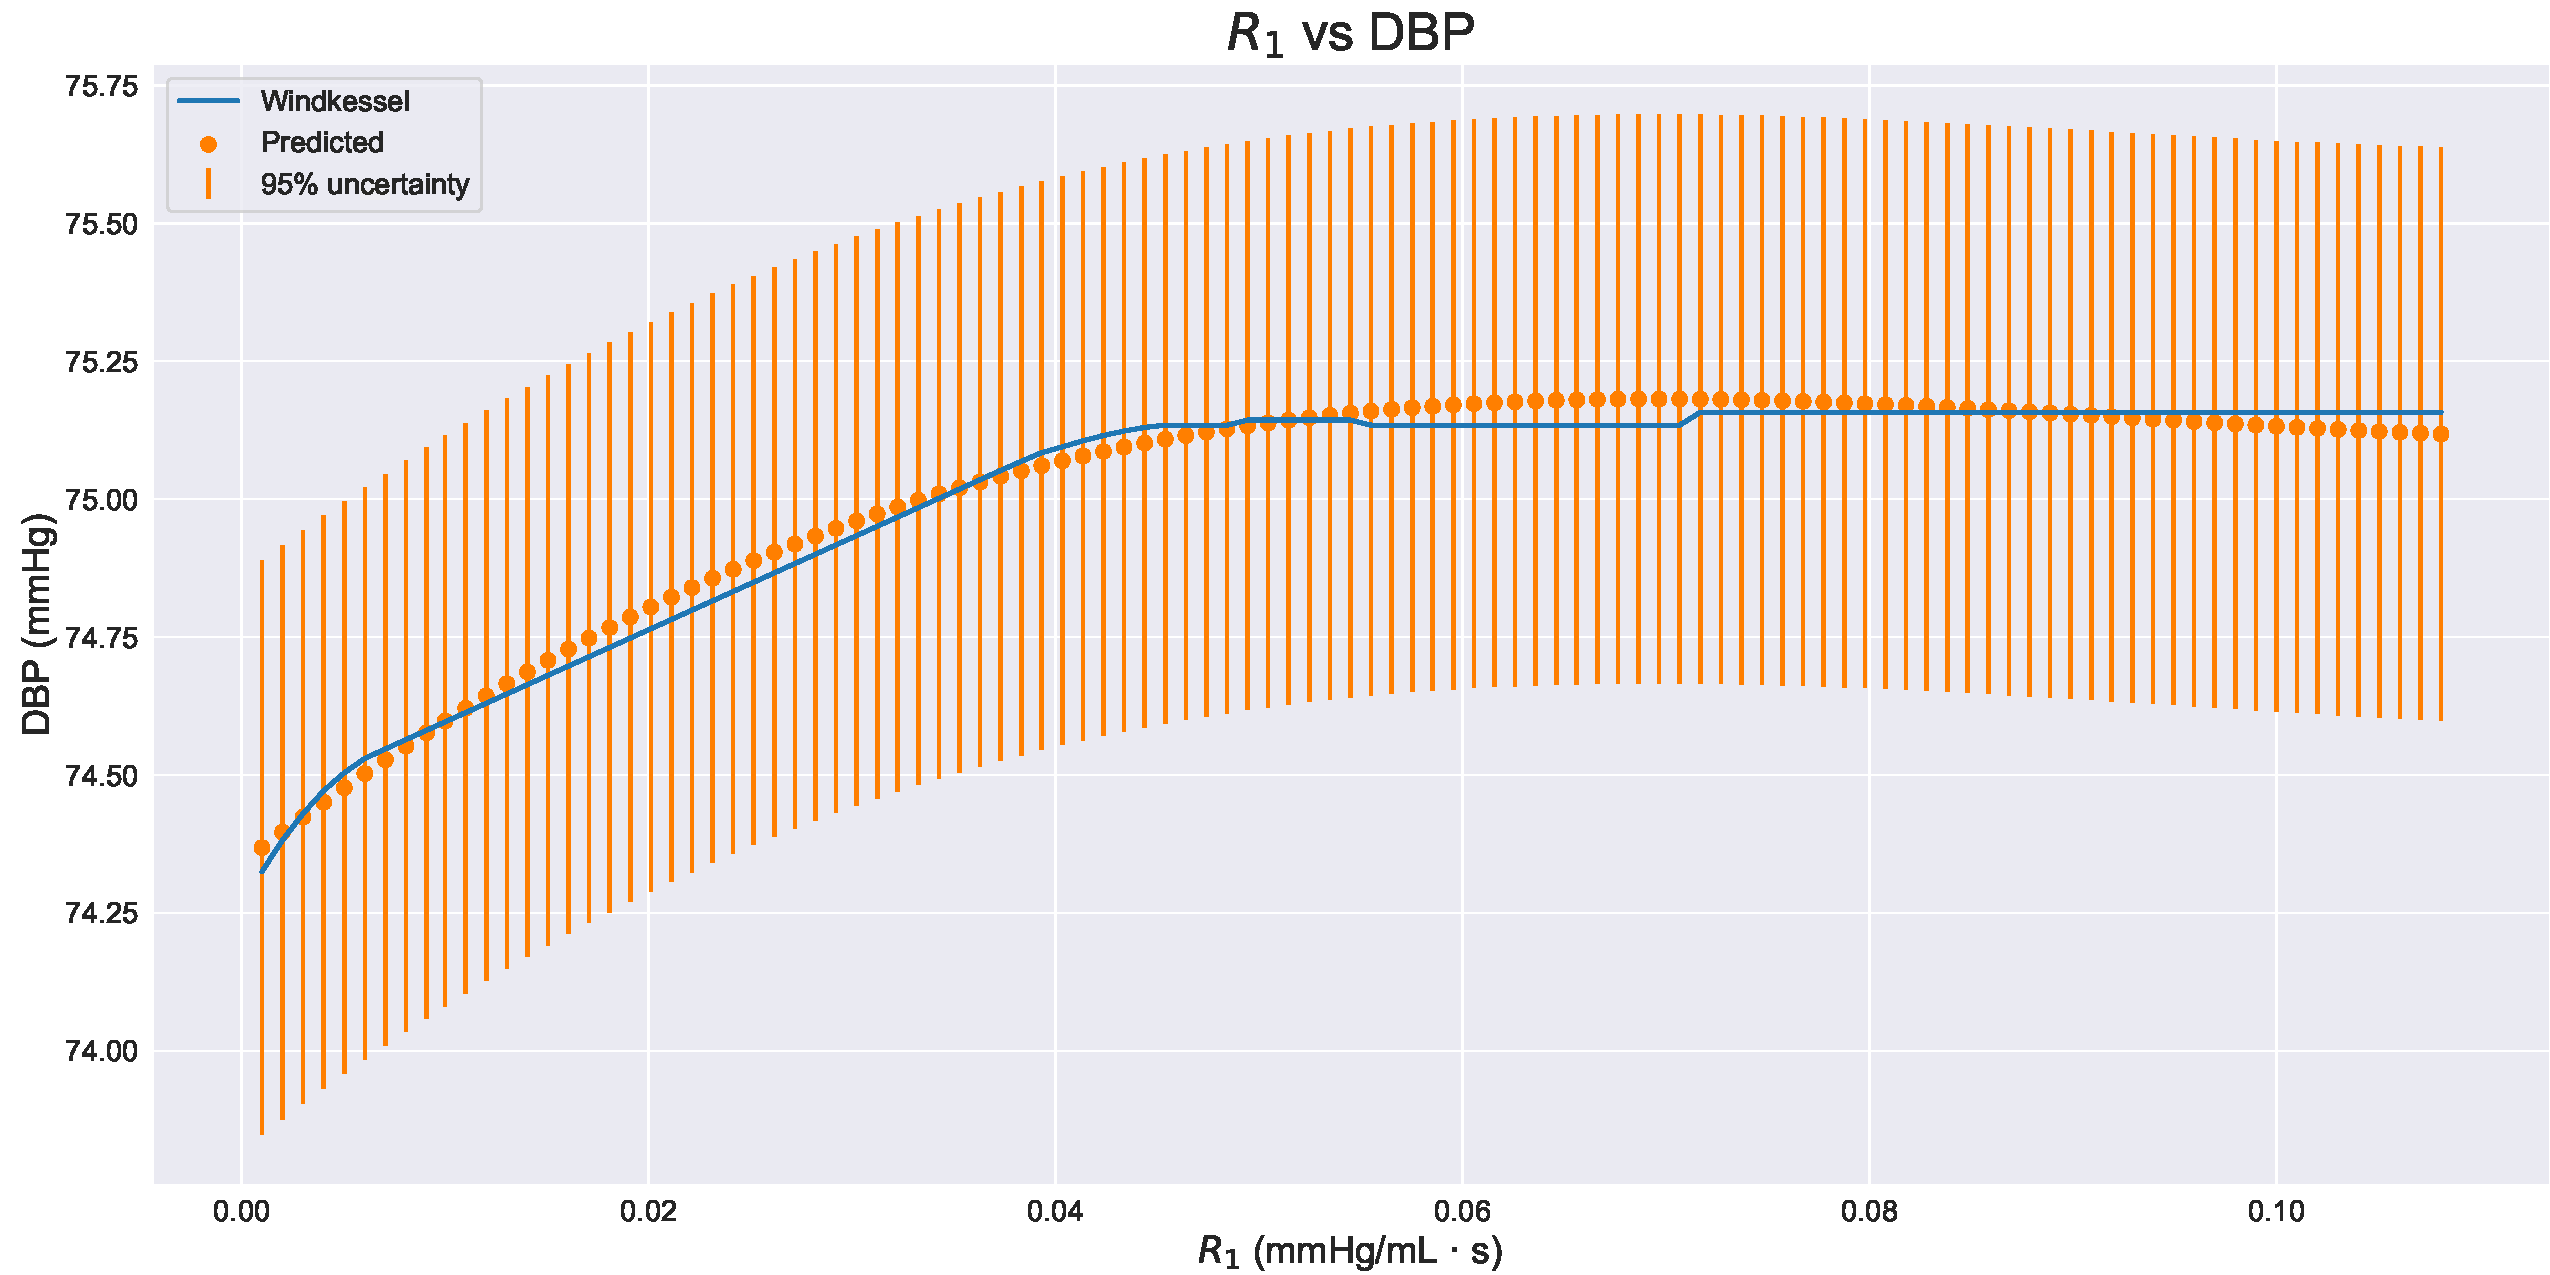
\includegraphics[width=1\textwidth]{images/Training (risultati)/DBP/DBP - R1 - full.pdf}
    \caption{Dipendenza di DBP da $R_1$ sull'intervallo di training e due intervalli attigui.}
    \label{DBP - R1 - full}
\end{figure}

\vspace{0.32cm}

\begin{figure}[!htb]
    \centering
    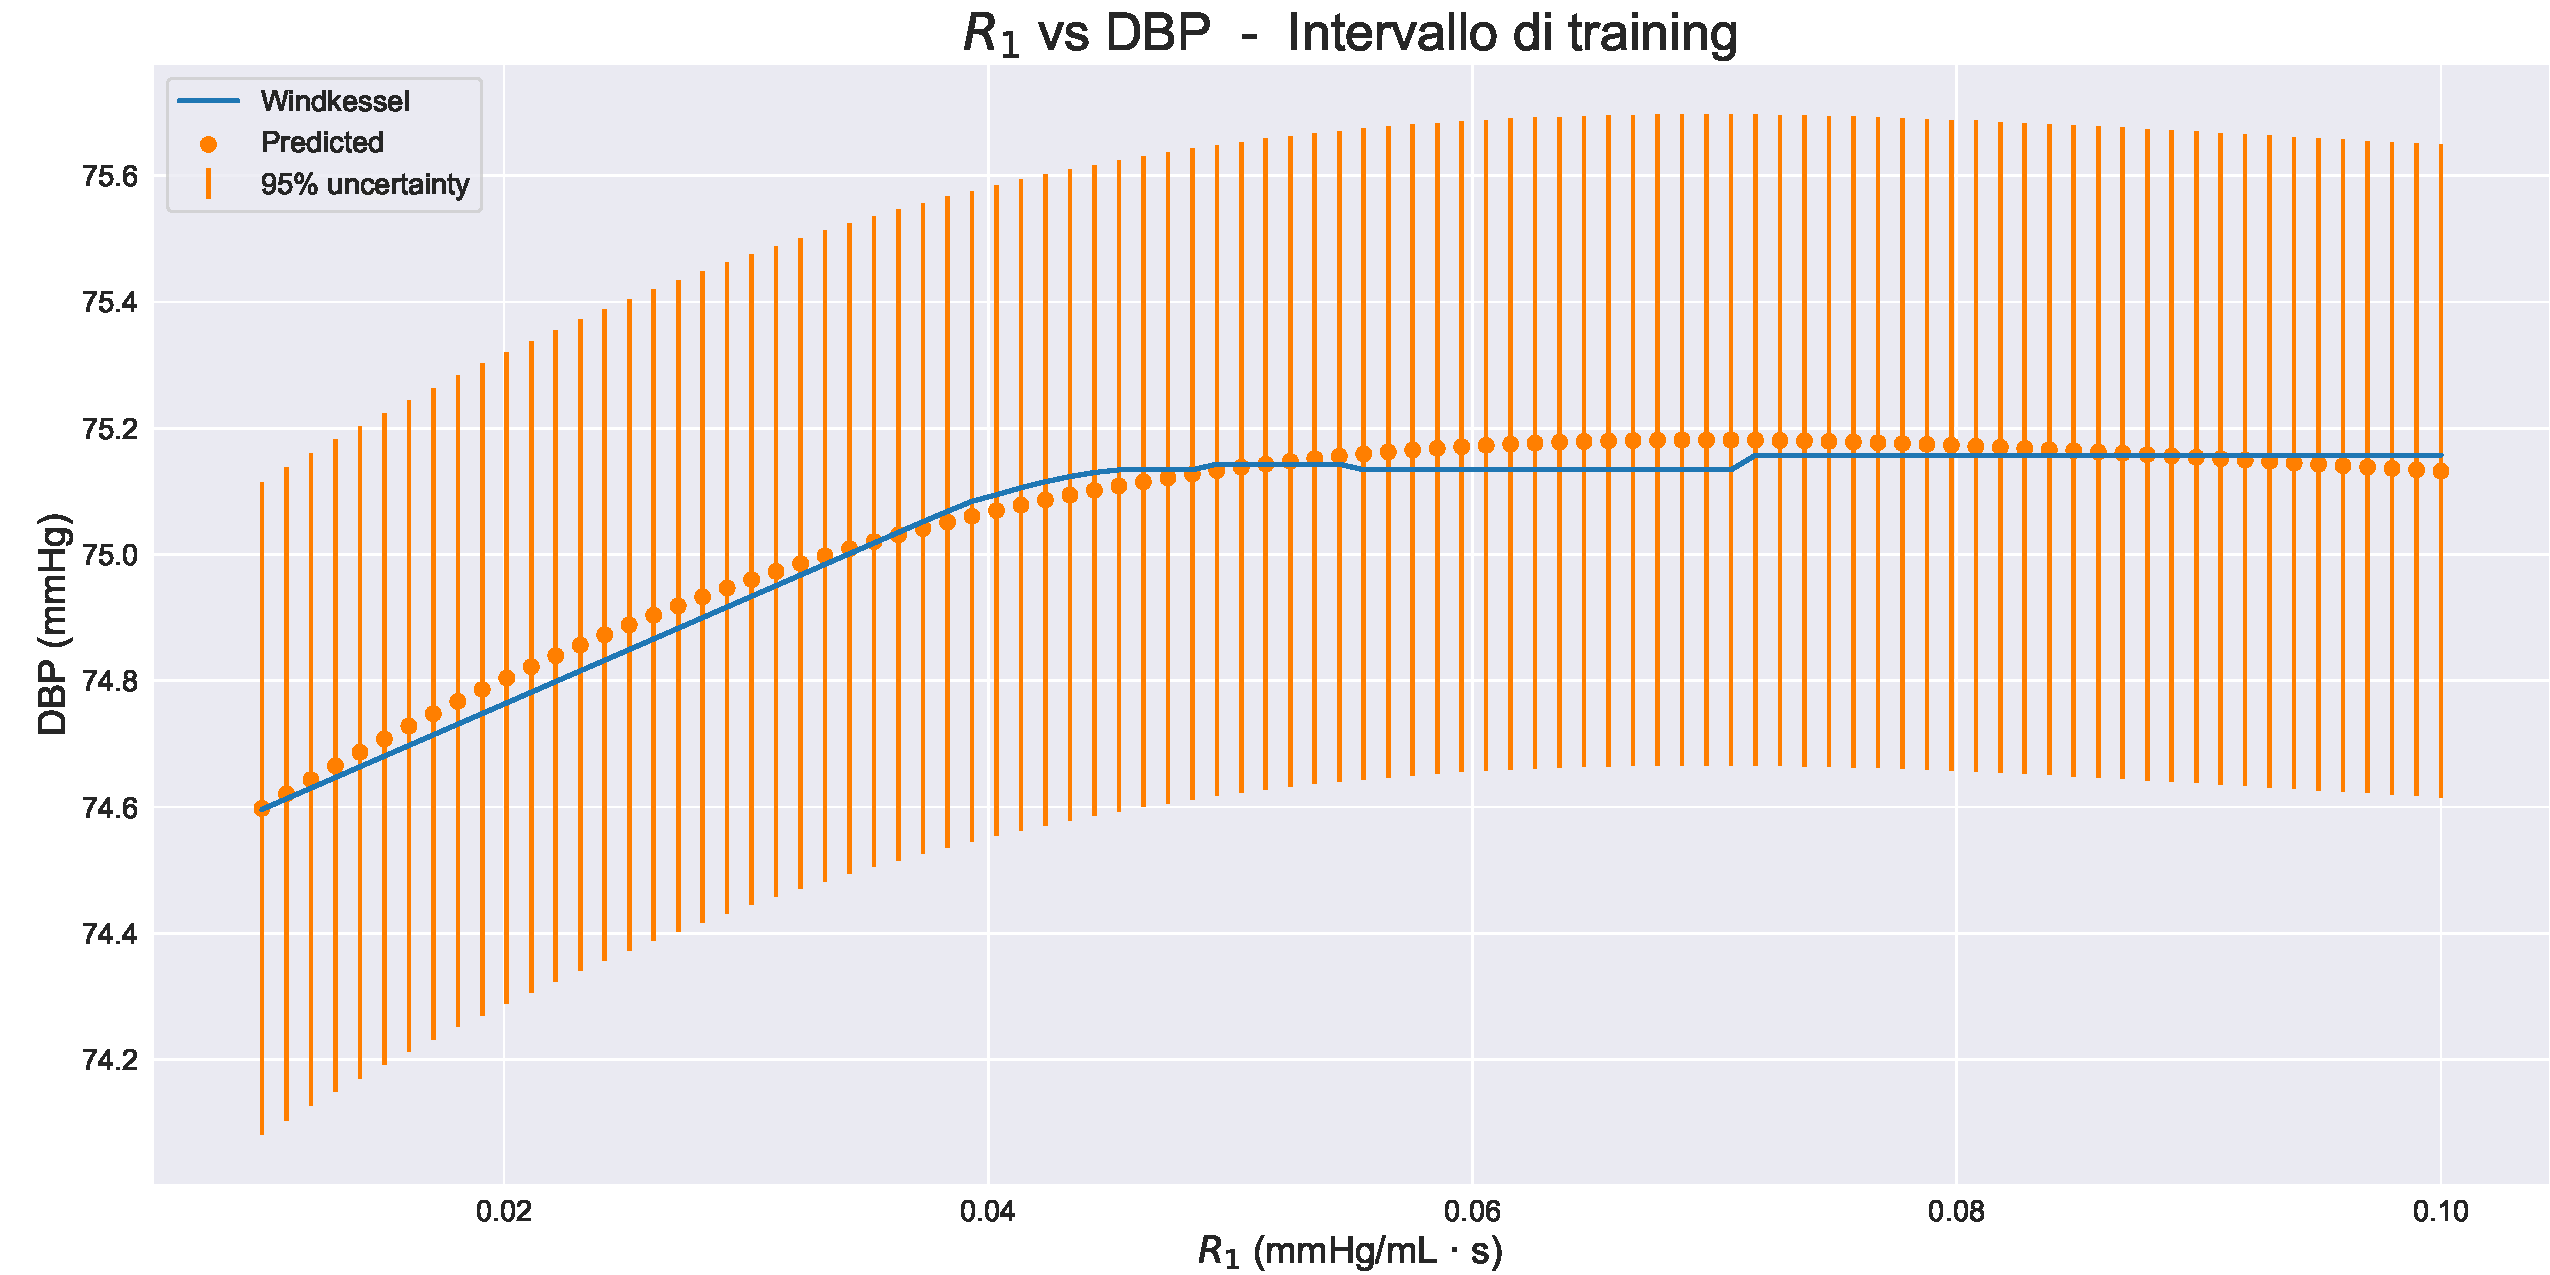
\includegraphics[width=1\textwidth]{images/Training (risultati)/DBP/DBP - R1 - training.pdf}
    \caption{Dipendenza di DBP da $R_1$ sull'intervallo di training.}
    \label{DBP - R1 - training}
\end{figure}

\begin{figure}
    \centering
    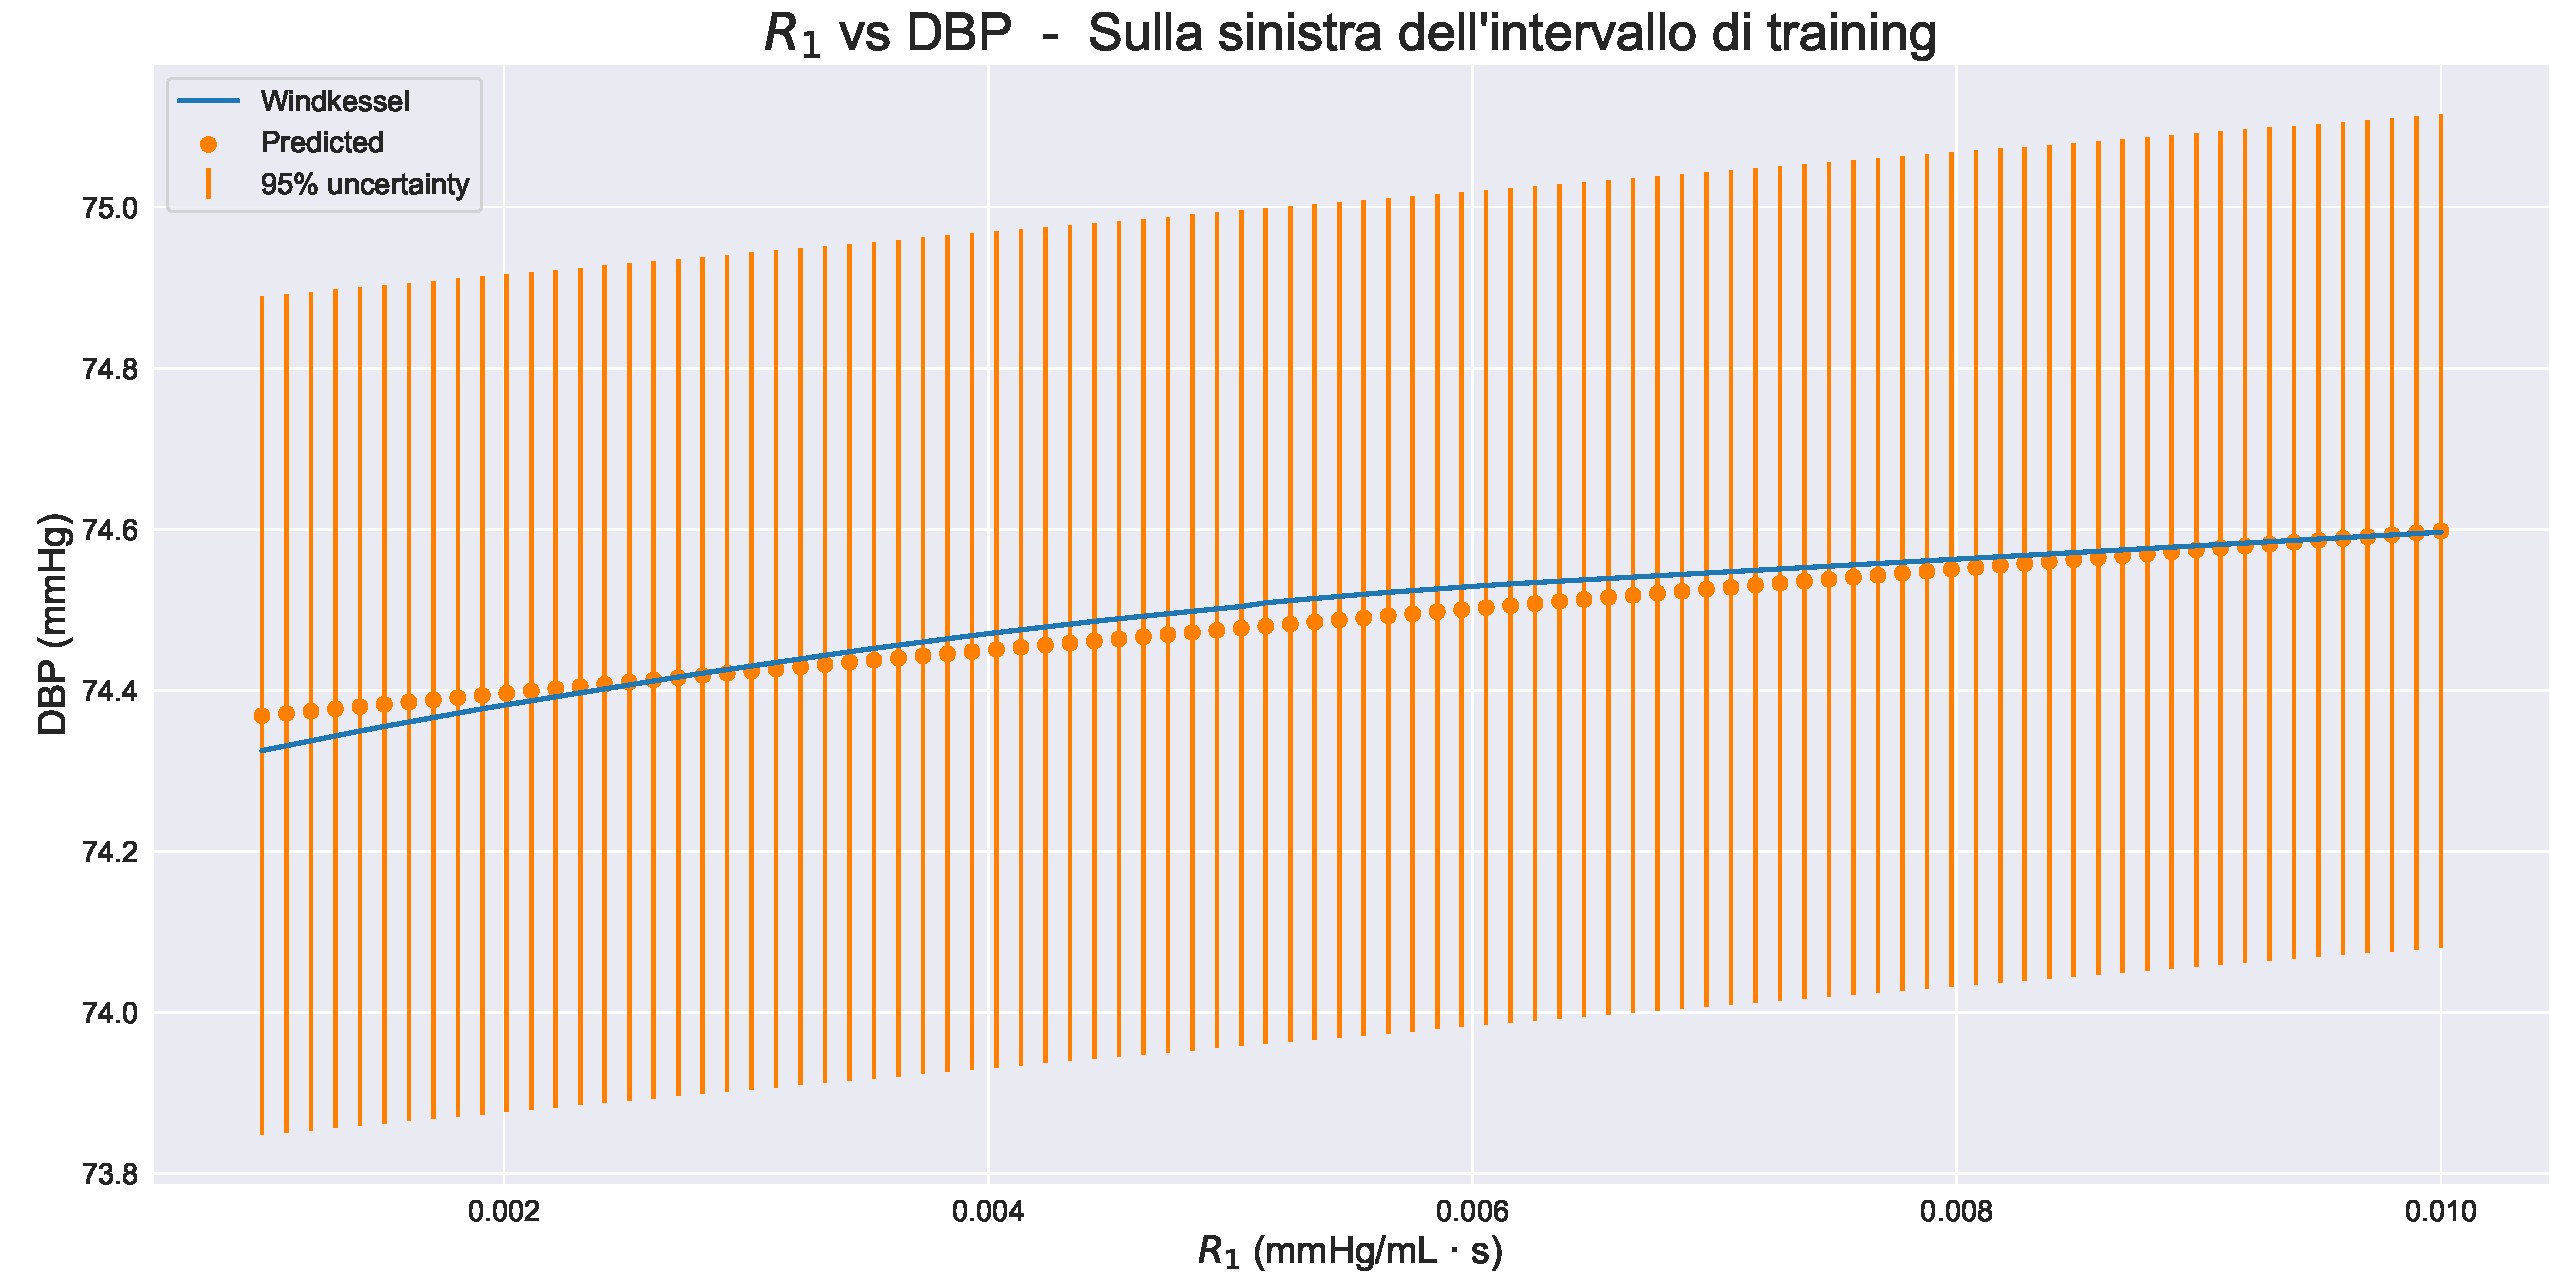
\includegraphics[width=1\textwidth]{images/Training (risultati)/DBP/DBP - R1 - sx.pdf}
    \caption{Dipendenza di DBP da $R_1$ sull'intervallo attiguo a sinistra dell'intervallo di training.}
    \label{DBP - R1 - sx}
\end{figure}



\begin{figure}
    \centering
    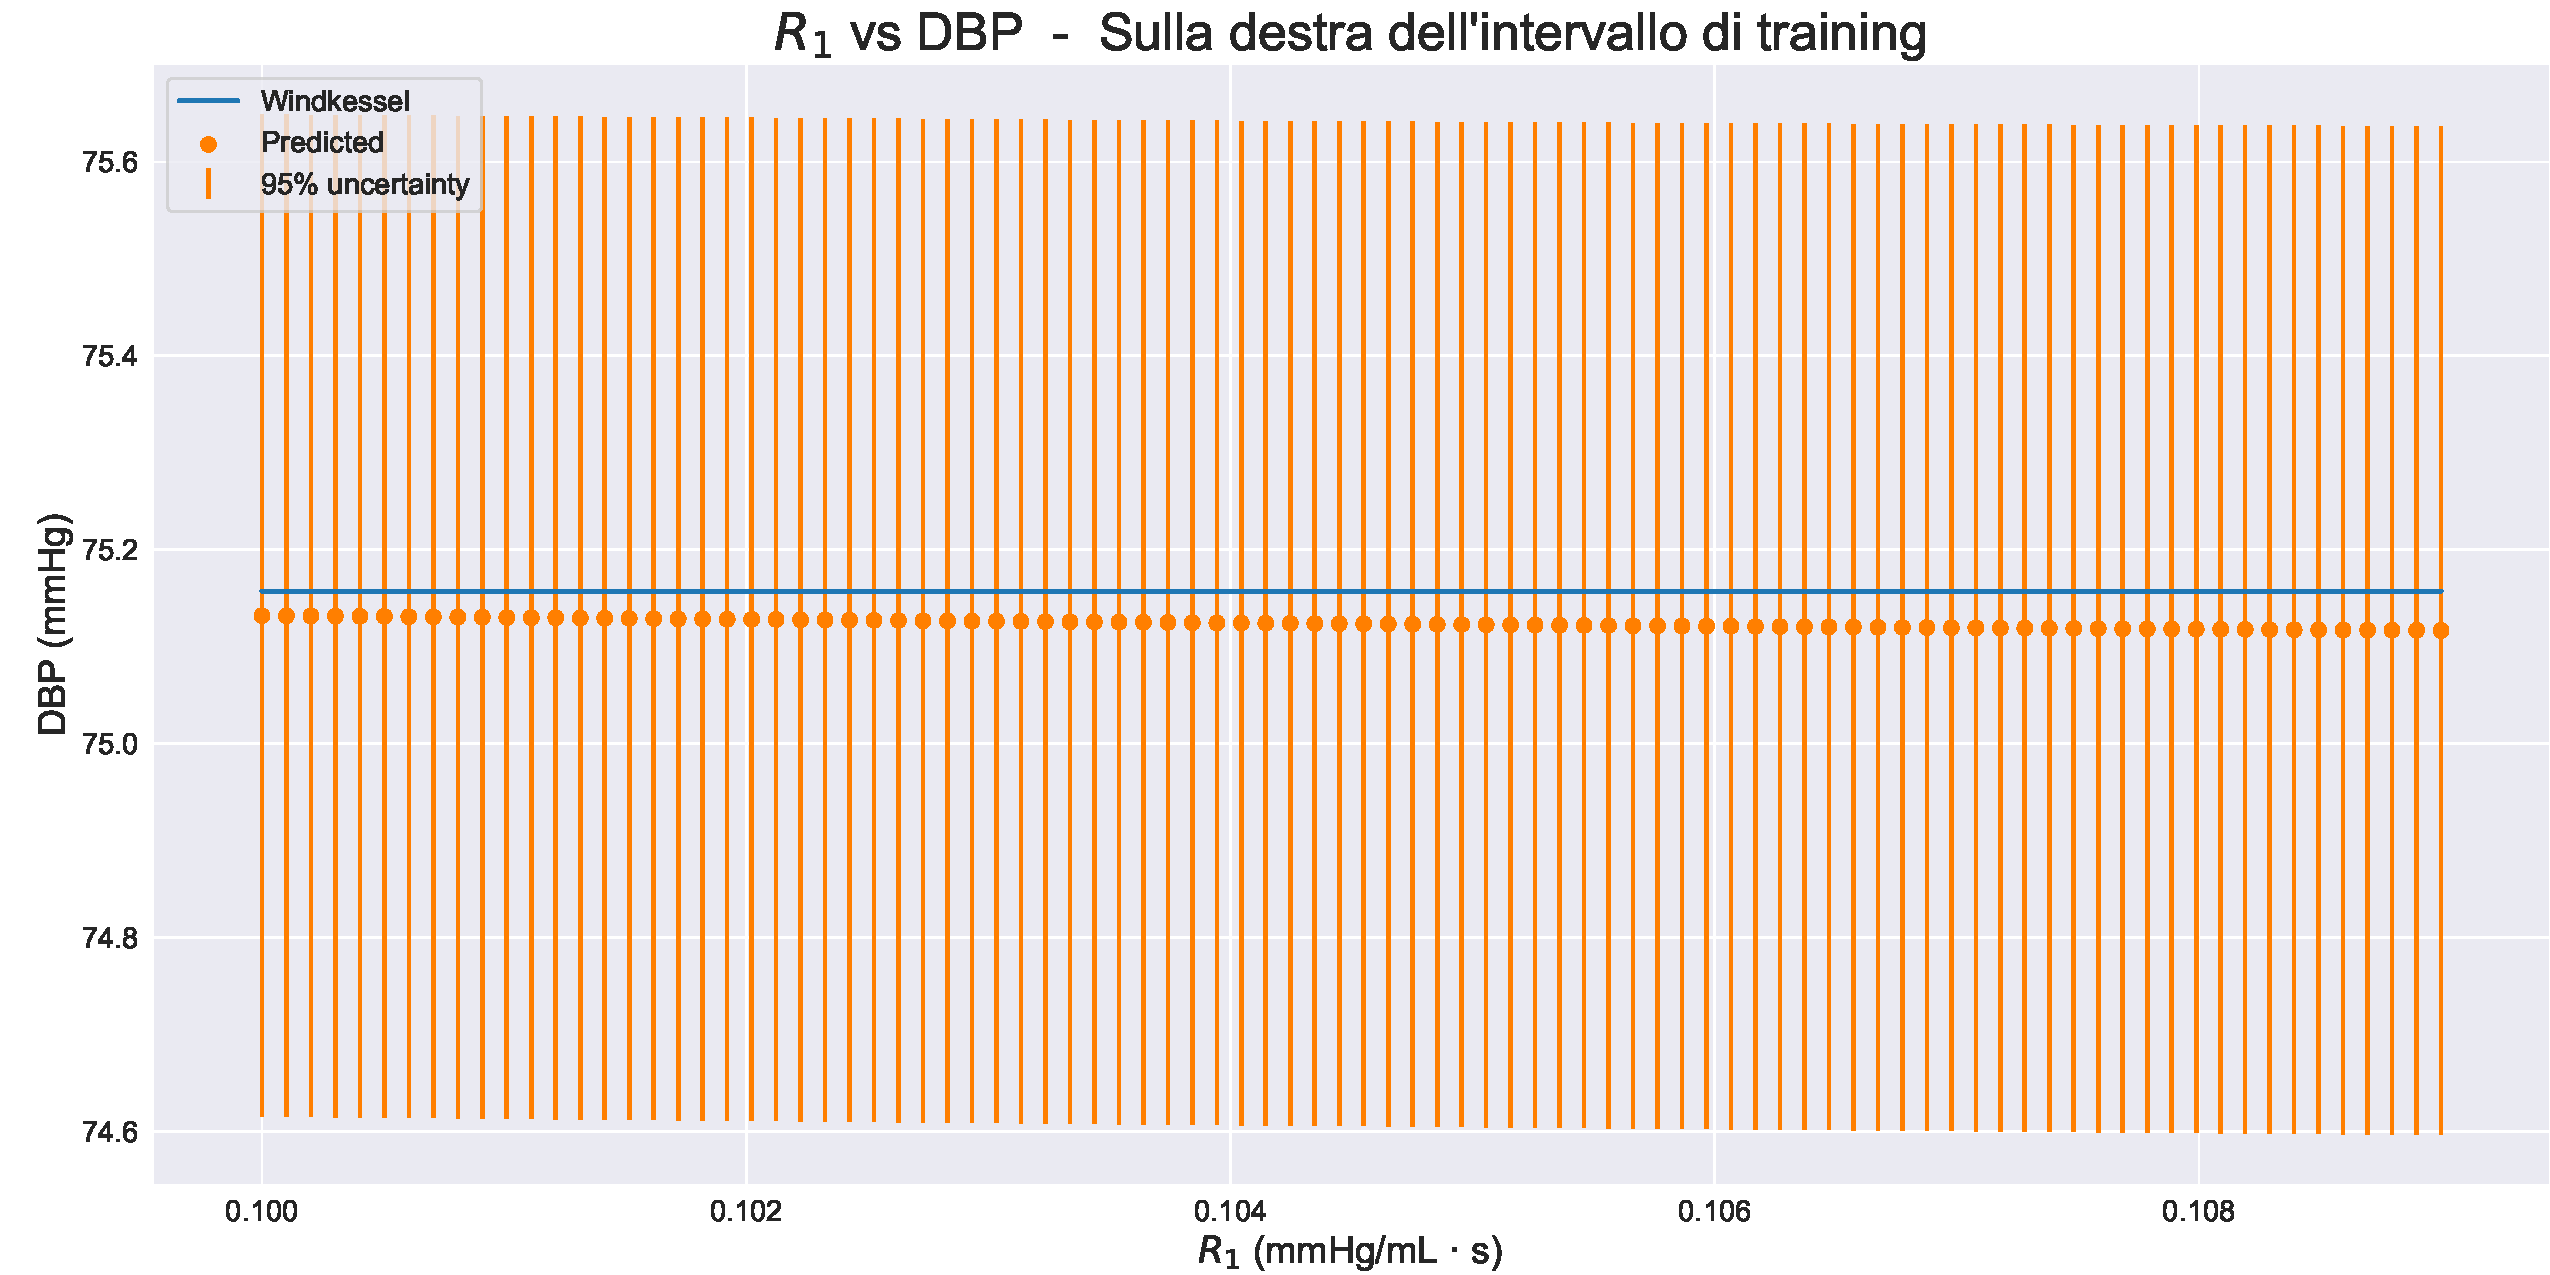
\includegraphics[width=1\textwidth]{images/Training (risultati)/DBP/DBP - R1 - dx.pdf}
    \caption{Dipendenza di DBP da $R_1$ sull'intervallo attiguo a destra dell'intervallo di training.}
    \label{DBP - R1 - dx}
\end{figure}



\newpage
% **********
% DBP - R2
% **********
\subsubsection{Dipendenza da $R_2$}
Il risultato complessivo è mostrato in figura \ref{DBP - R2 - full}, il risultato nel solo intervallo di training in \ref{DBP - R2 - training}, il risultato nei singoli intervalli attigui in \ref{DBP - R2 - sx} e \ref{DBP - R2 - dx}. Anche in questo caso si hanno predizioni molto precise. A prima vista sembra che le barre di errore non compaiano, in realtà sono molto brevi rispetto alla scala usata. Infatti nei grafici in cui si plottano solo gli intervalli attigui le barre di errore ricompaiono e mostrano che l'errore è minore di una unità.

\vspace{1cm}

\begin{figure}[!htb]
    \centering
    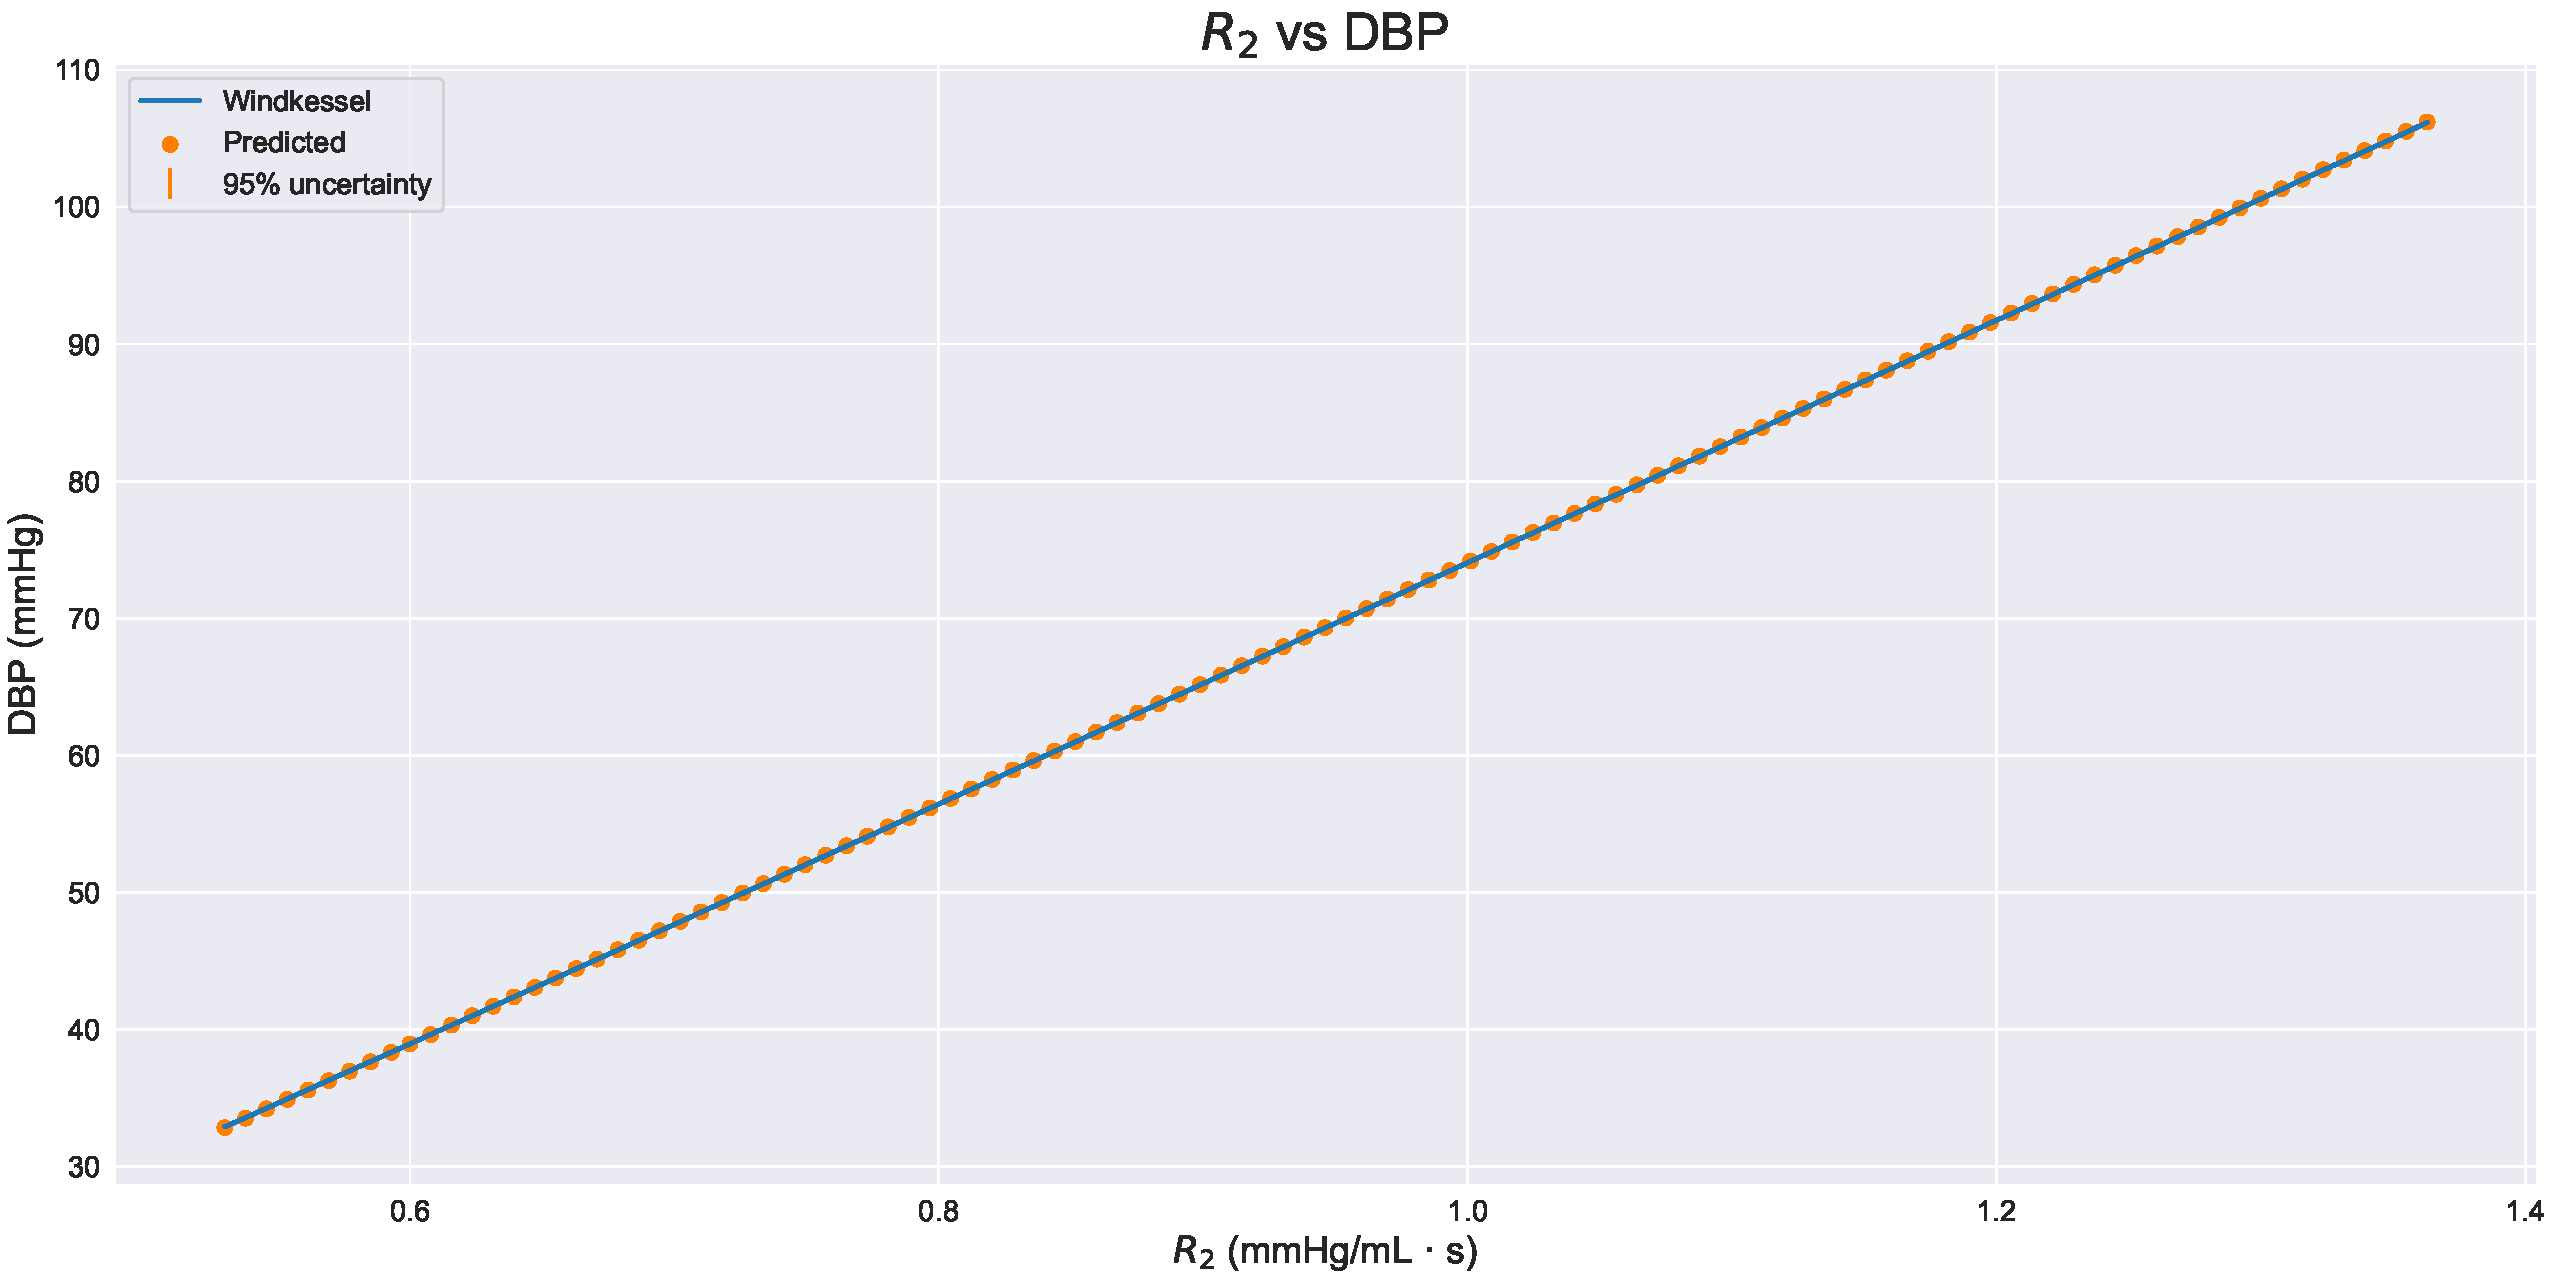
\includegraphics[width=1\textwidth]{images/Training (risultati)/DBP/DBP - R2 - full.pdf}
    \caption{Dipendenza di DBP da $R_2$ sull'intervallo di training e due intervalli attigui.}
    \label{DBP - R2 - full}
\end{figure}

\vspace{0.34cm}

\begin{figure}[!htb]
    \centering
    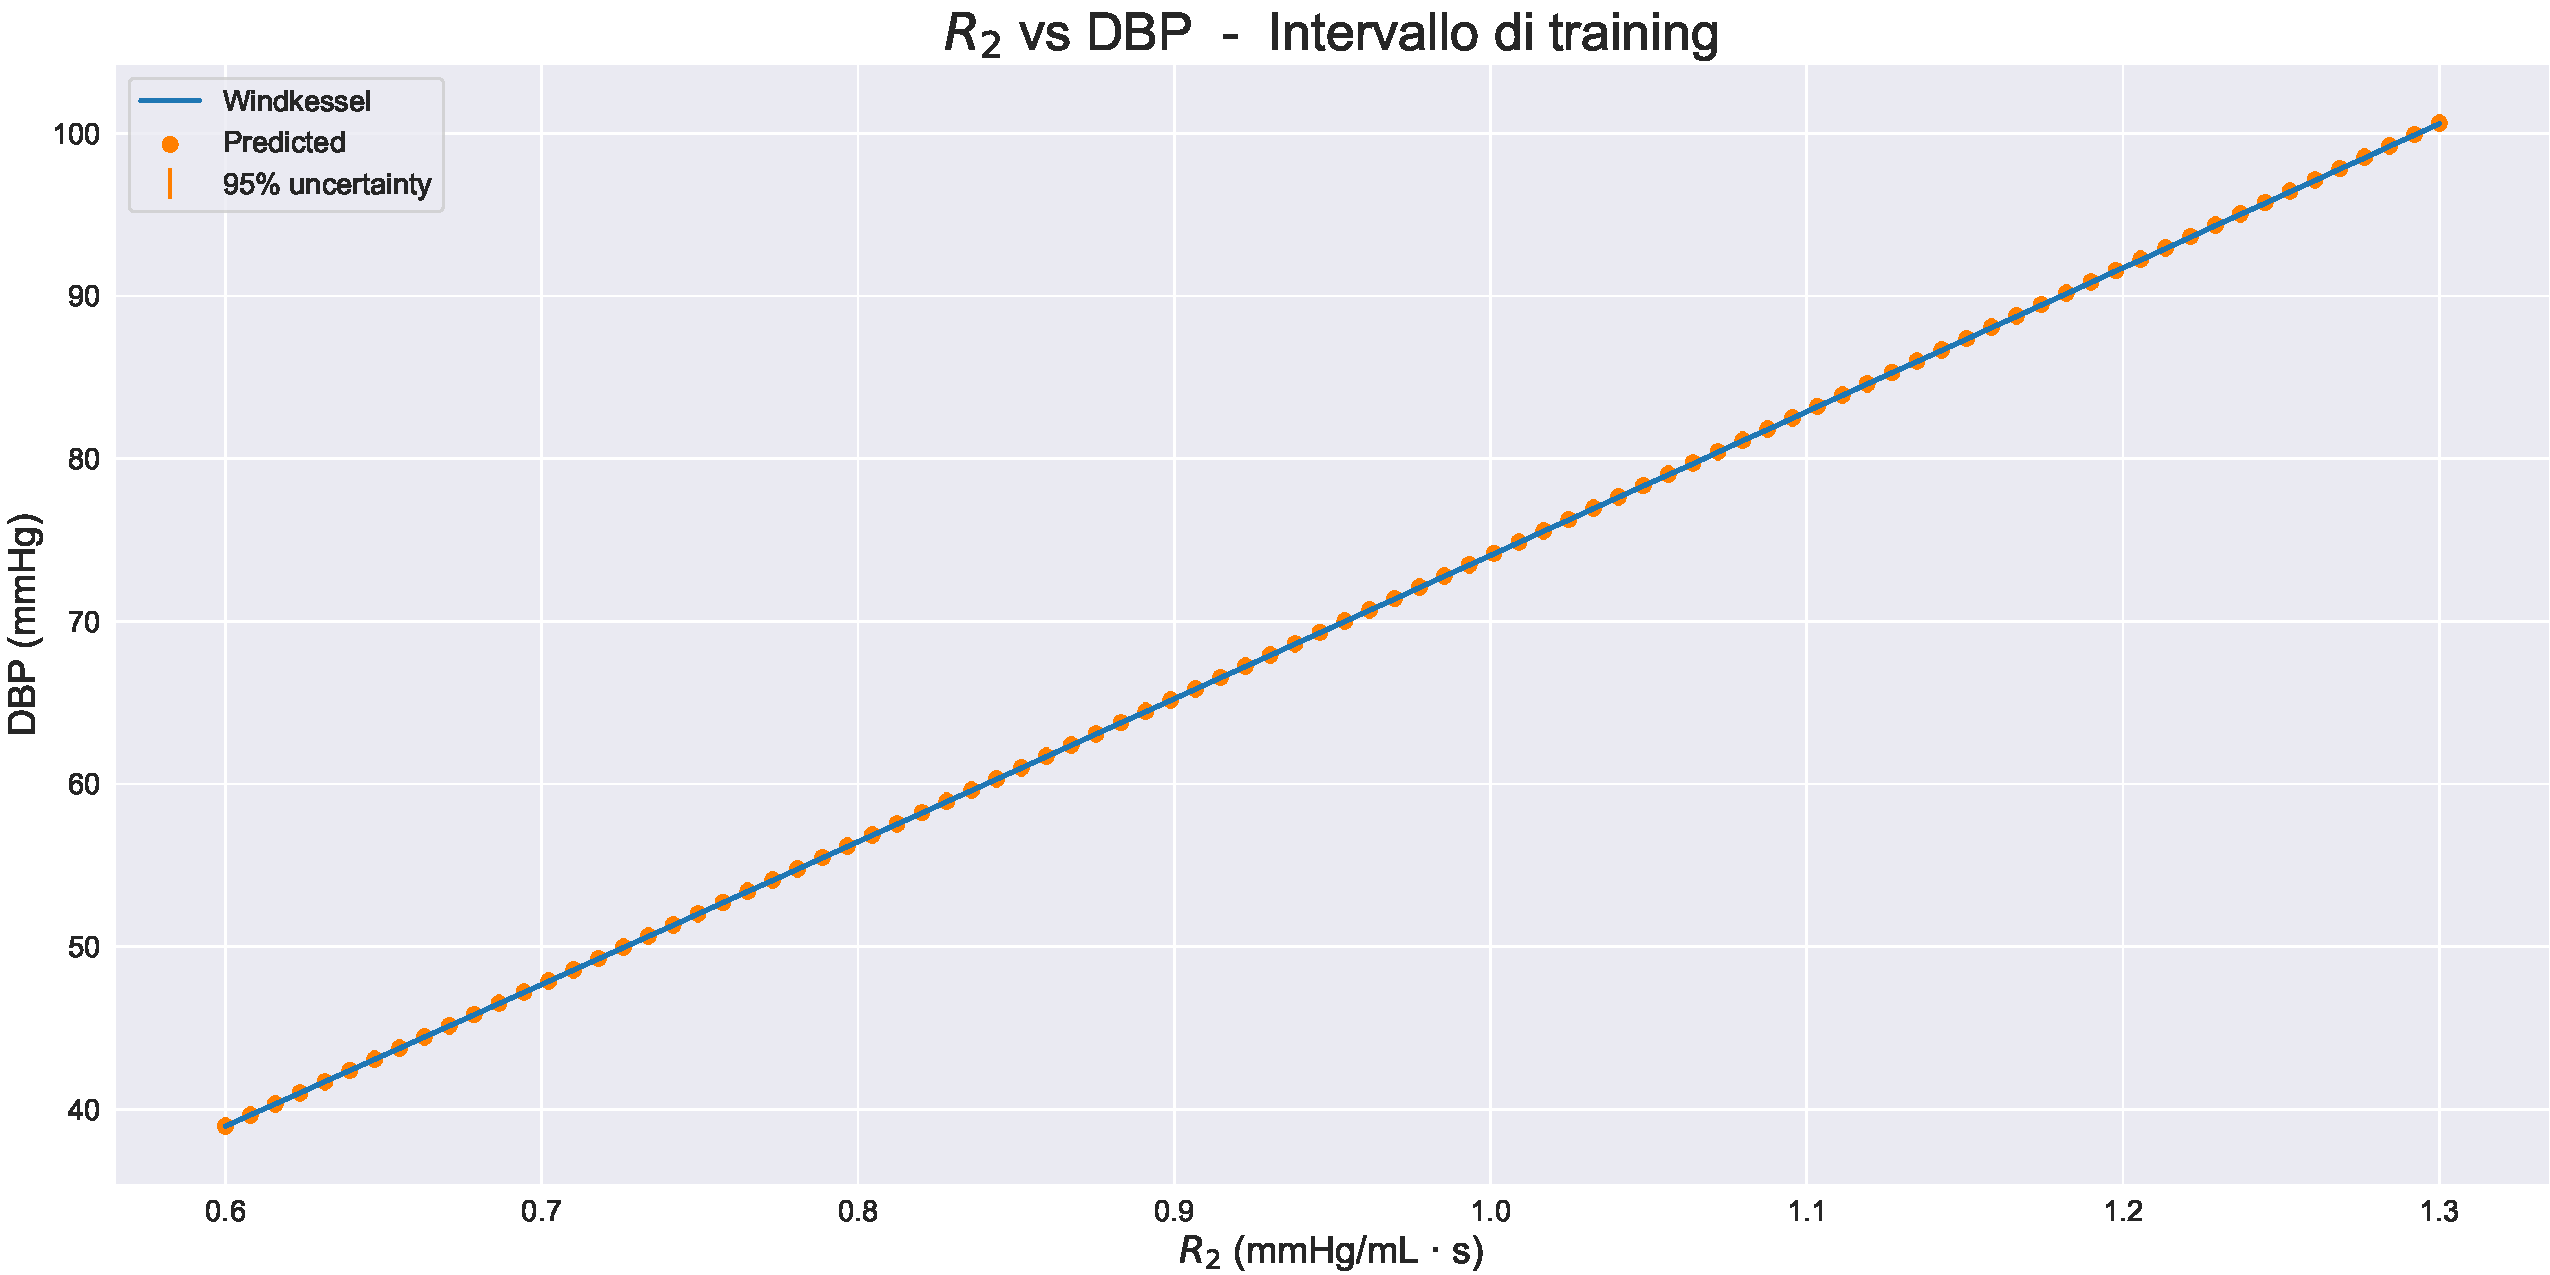
\includegraphics[width=1\textwidth]{images/Training (risultati)/DBP/DBP - R2 - training.pdf}
    \caption{Dipendenza di DBP da $R_2$ sull'intervallo di training.}
    \label{DBP - R2 - training}
\end{figure}

\begin{figure}
    \centering
    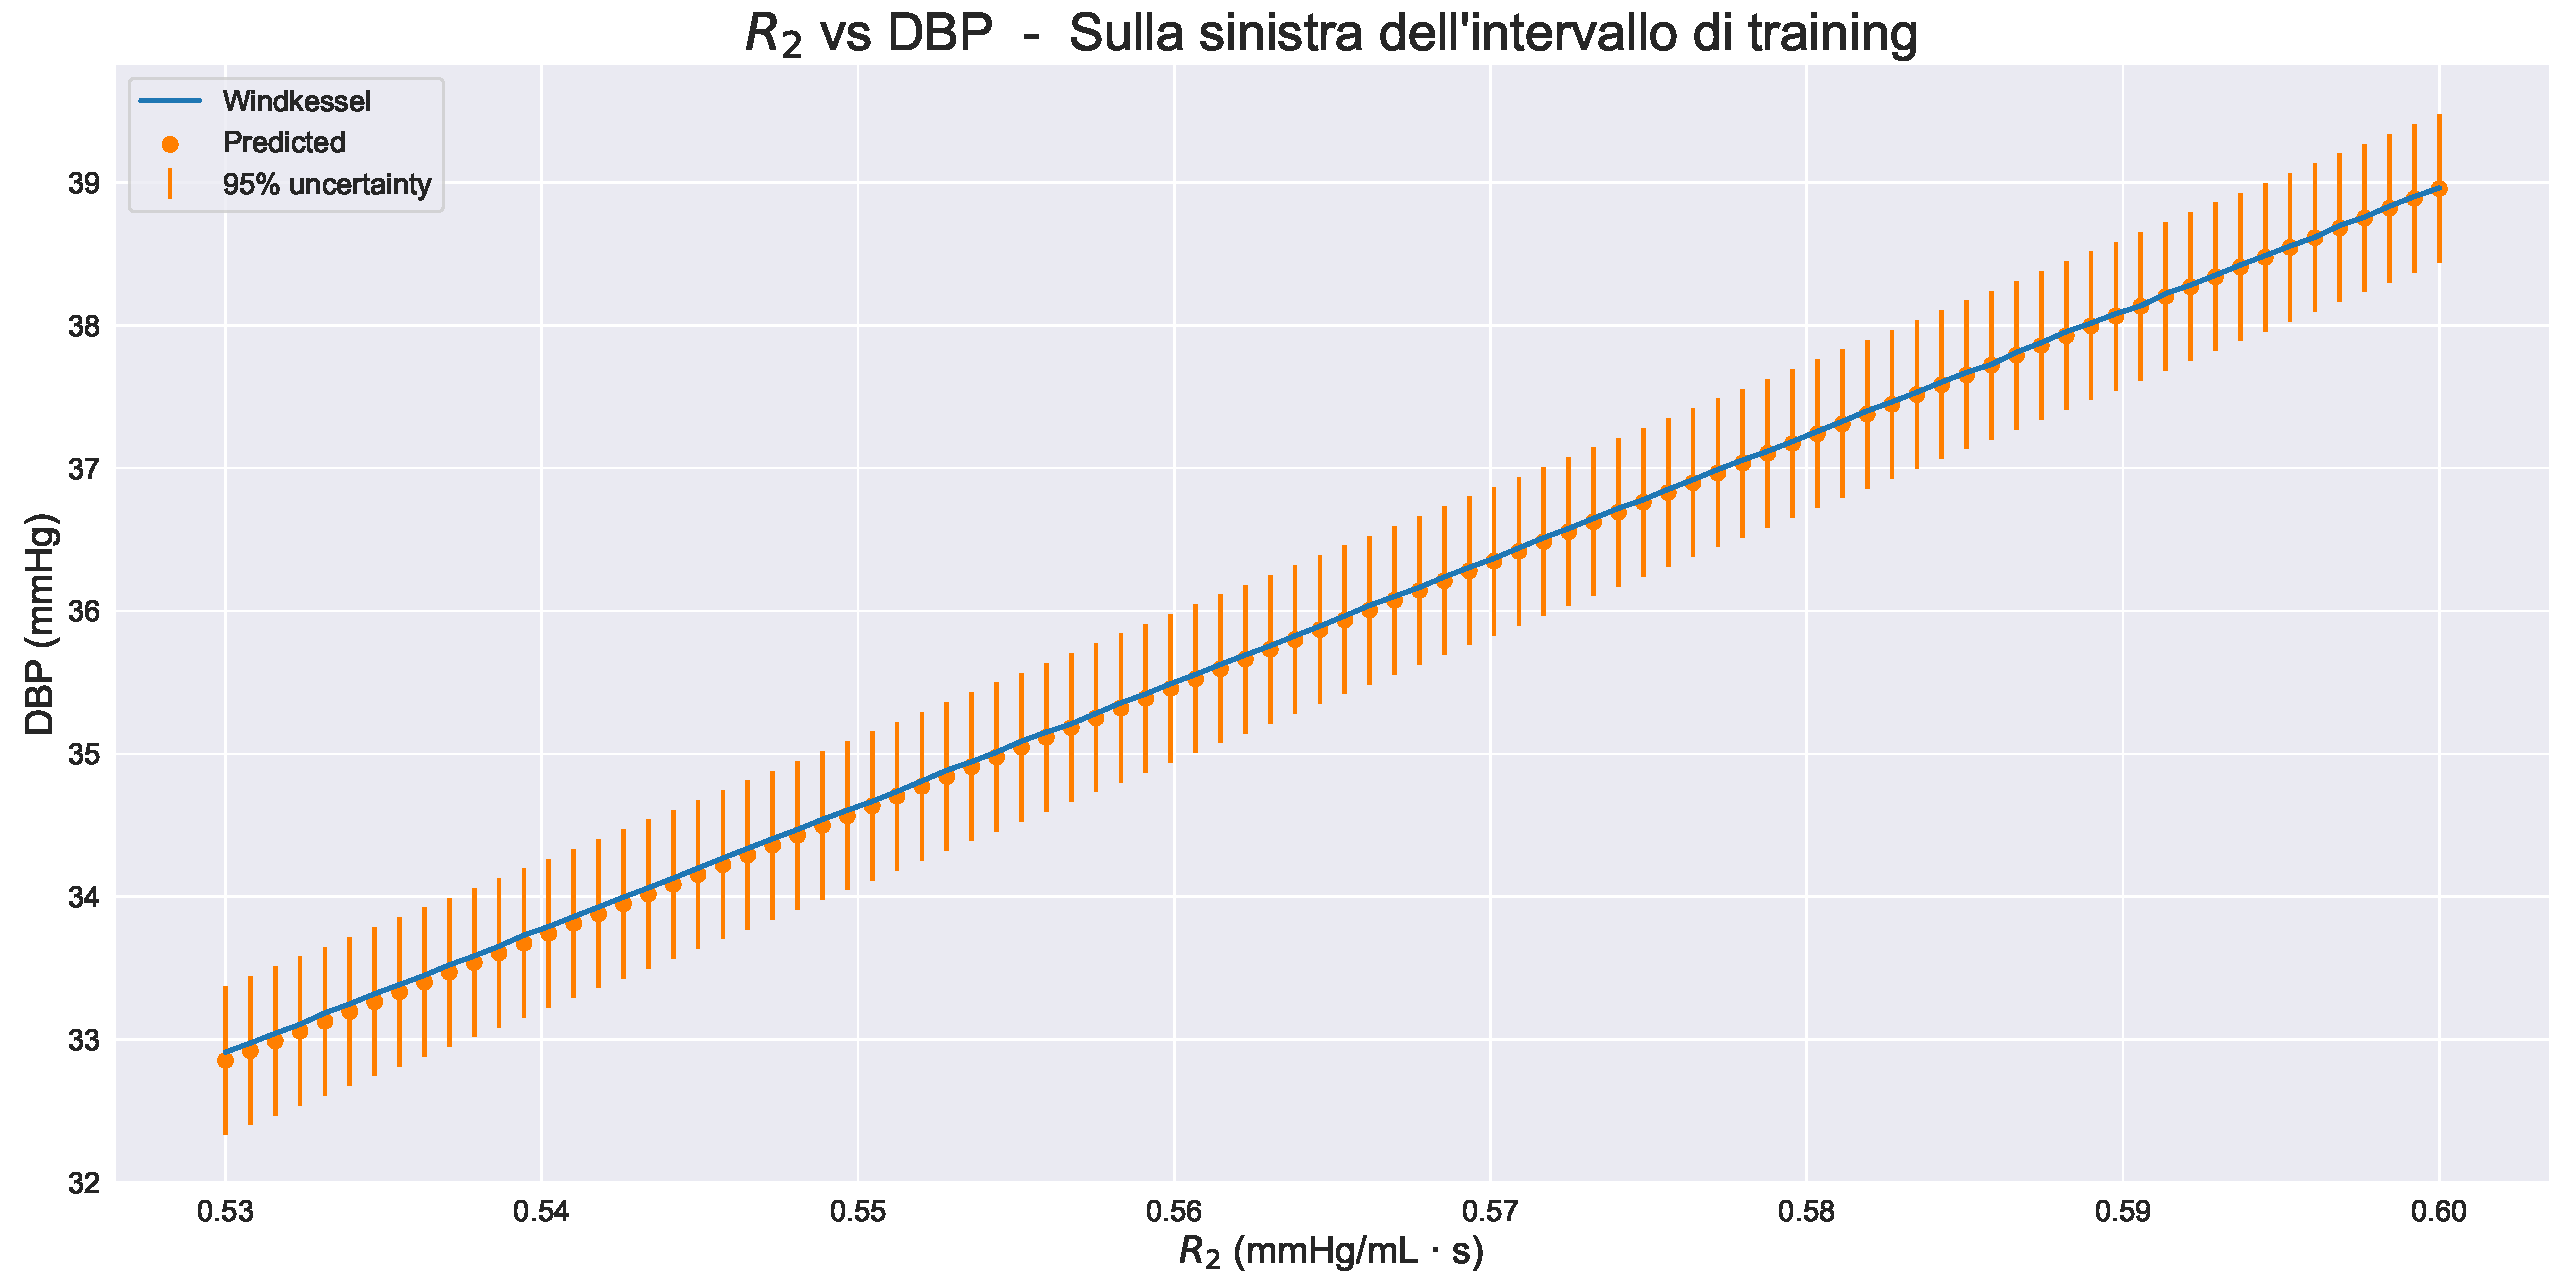
\includegraphics[width=1\textwidth]{images/Training (risultati)/DBP/DBP - R2 - sx.pdf}
    \caption{Dipendenza di DBP da $R_2$ sull'intervallo attiguo a sinistra dell'intervallo di training.}
    \label{DBP - R2 - sx}
\end{figure}


\begin{figure}
    \centering
    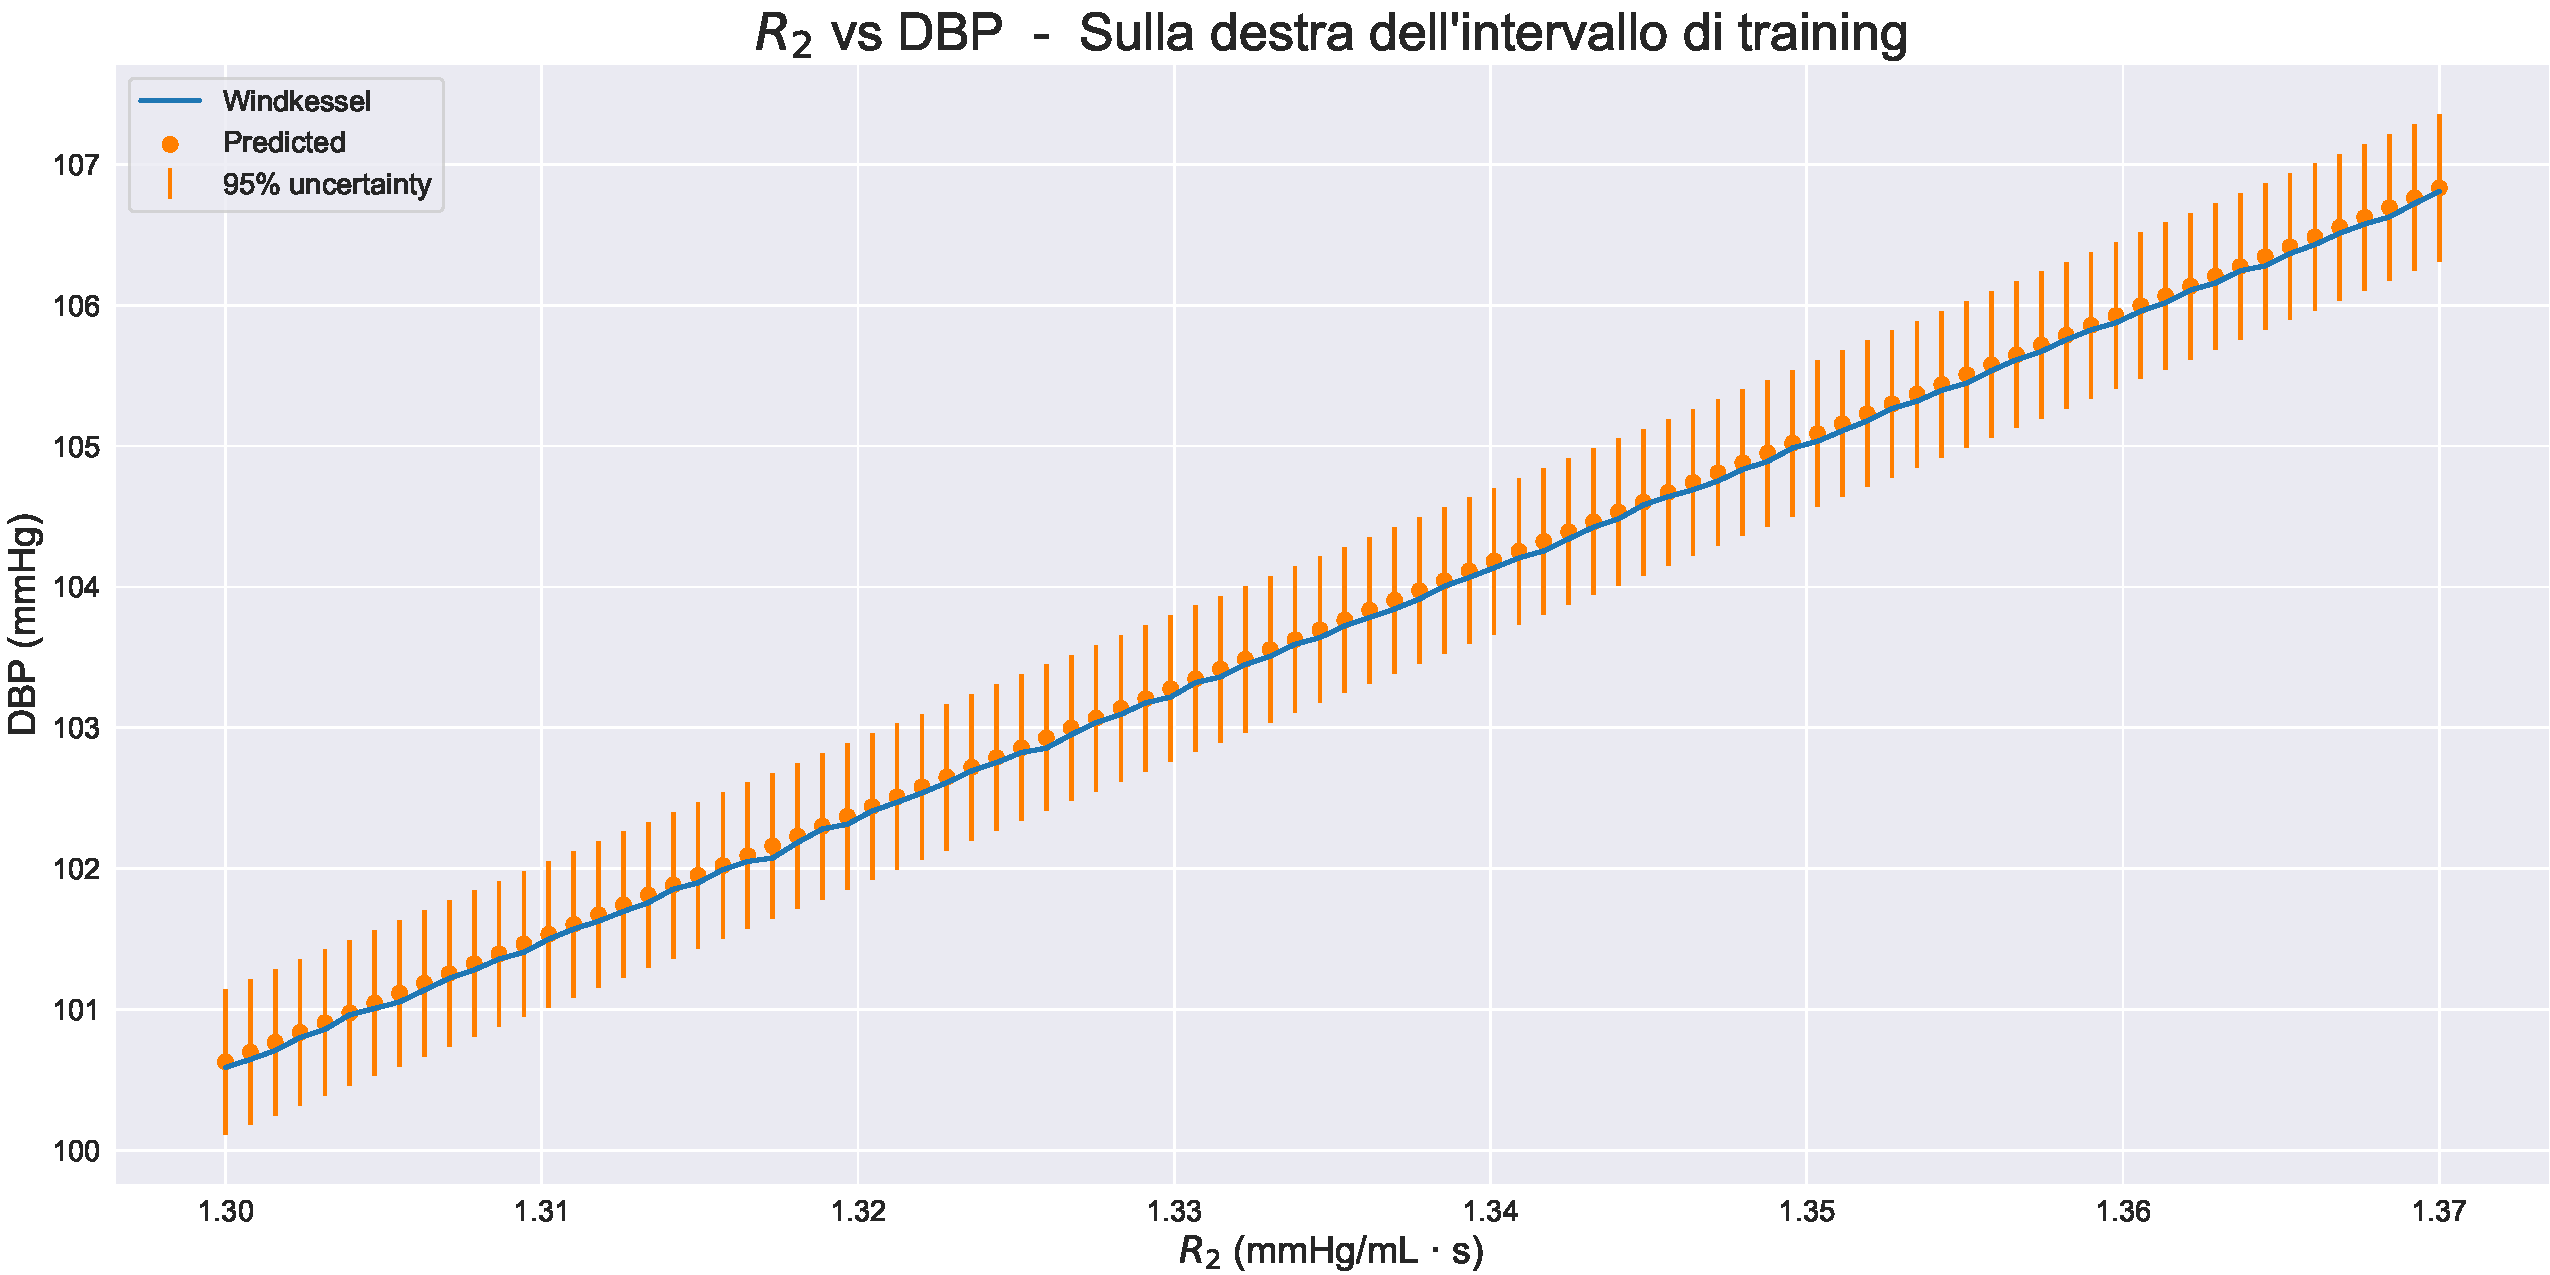
\includegraphics[width=1\textwidth]{images/Training (risultati)/DBP/DBP - R2 - dx.pdf}
    \caption{Dipendenza di DBP da $R_2$ sull'intervallo attiguo a destra dell'intervallo di training.}
    \label{DBP - R2 - dx}
\end{figure}







\newpage
%******************************
%*********** PP **************
%******************************
\subsection{Pulse pressure (PP)}
Viene imposto $\text{lr}=0.05$ e viene usato l'early stopper \textit{GLEarlyStoppingCriterion} con parametri: $\alpha = 5$, $\text{patience}=3$.


% **********
% PP - loss
% **********
\subsubsection{Training e validation loss}
Il training ha necessitato novantatre EPOCHS, ha concluso con $\text{R2Score}=0.9994$, $\text{MeanSquaredError}=0.0006$. In figura \ref{PP - loss} viene mostrato l'andamento del training e validation loss con MSE e R2Score; in verde l'andamento dell'early stopper.
\begin{figure}[h]
    \centering
    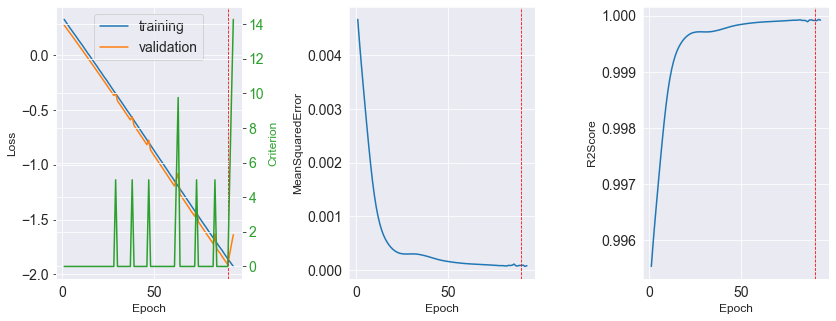
\includegraphics[width=1\textwidth]{images/Training (risultati)/PP/PP - loss.png}
    \caption{PP: andamento del training e validation loss, early stopper, R2Score e MSE.}
    \label{PP - loss}
\end{figure}

\vspace{-0.5cm}

% **********
% PP - inference
% **********
\subsubsection{Approssimazione dei dati di input}
In figura \ref{PP - inference} viene mostrato come le predizioni approssimano i dati di input. La lunghezza delle barre di errore è $0.0034$.

\begin{figure}[h]
    \centering
    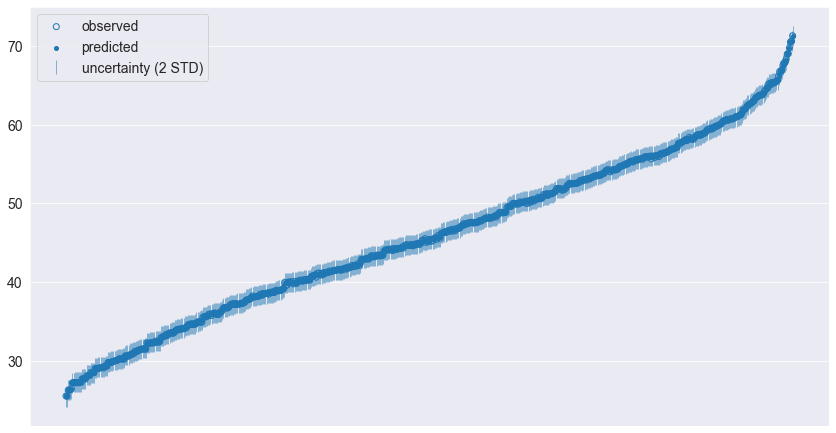
\includegraphics[width=1\textwidth]{images/Training (risultati)/PP/PP - inference.png}
    \caption{PP: predizioni sui dati di input.}
    \label{PP - inference}
\end{figure}



% **********
% PP - C
% **********
\subsubsection{Dipendenza da $C$}
Il risultato complessivo è mostrato in figura \ref{PP - C - full}, il risultato nel solo intervallo di training in \ref{PP - C - training}, il risultato nei singoli intervalli attigui in \ref{PP - C - sx} e \ref{PP - C - dx}.

\vspace{1cm}

\begin{figure}[!htb]
    \centering
    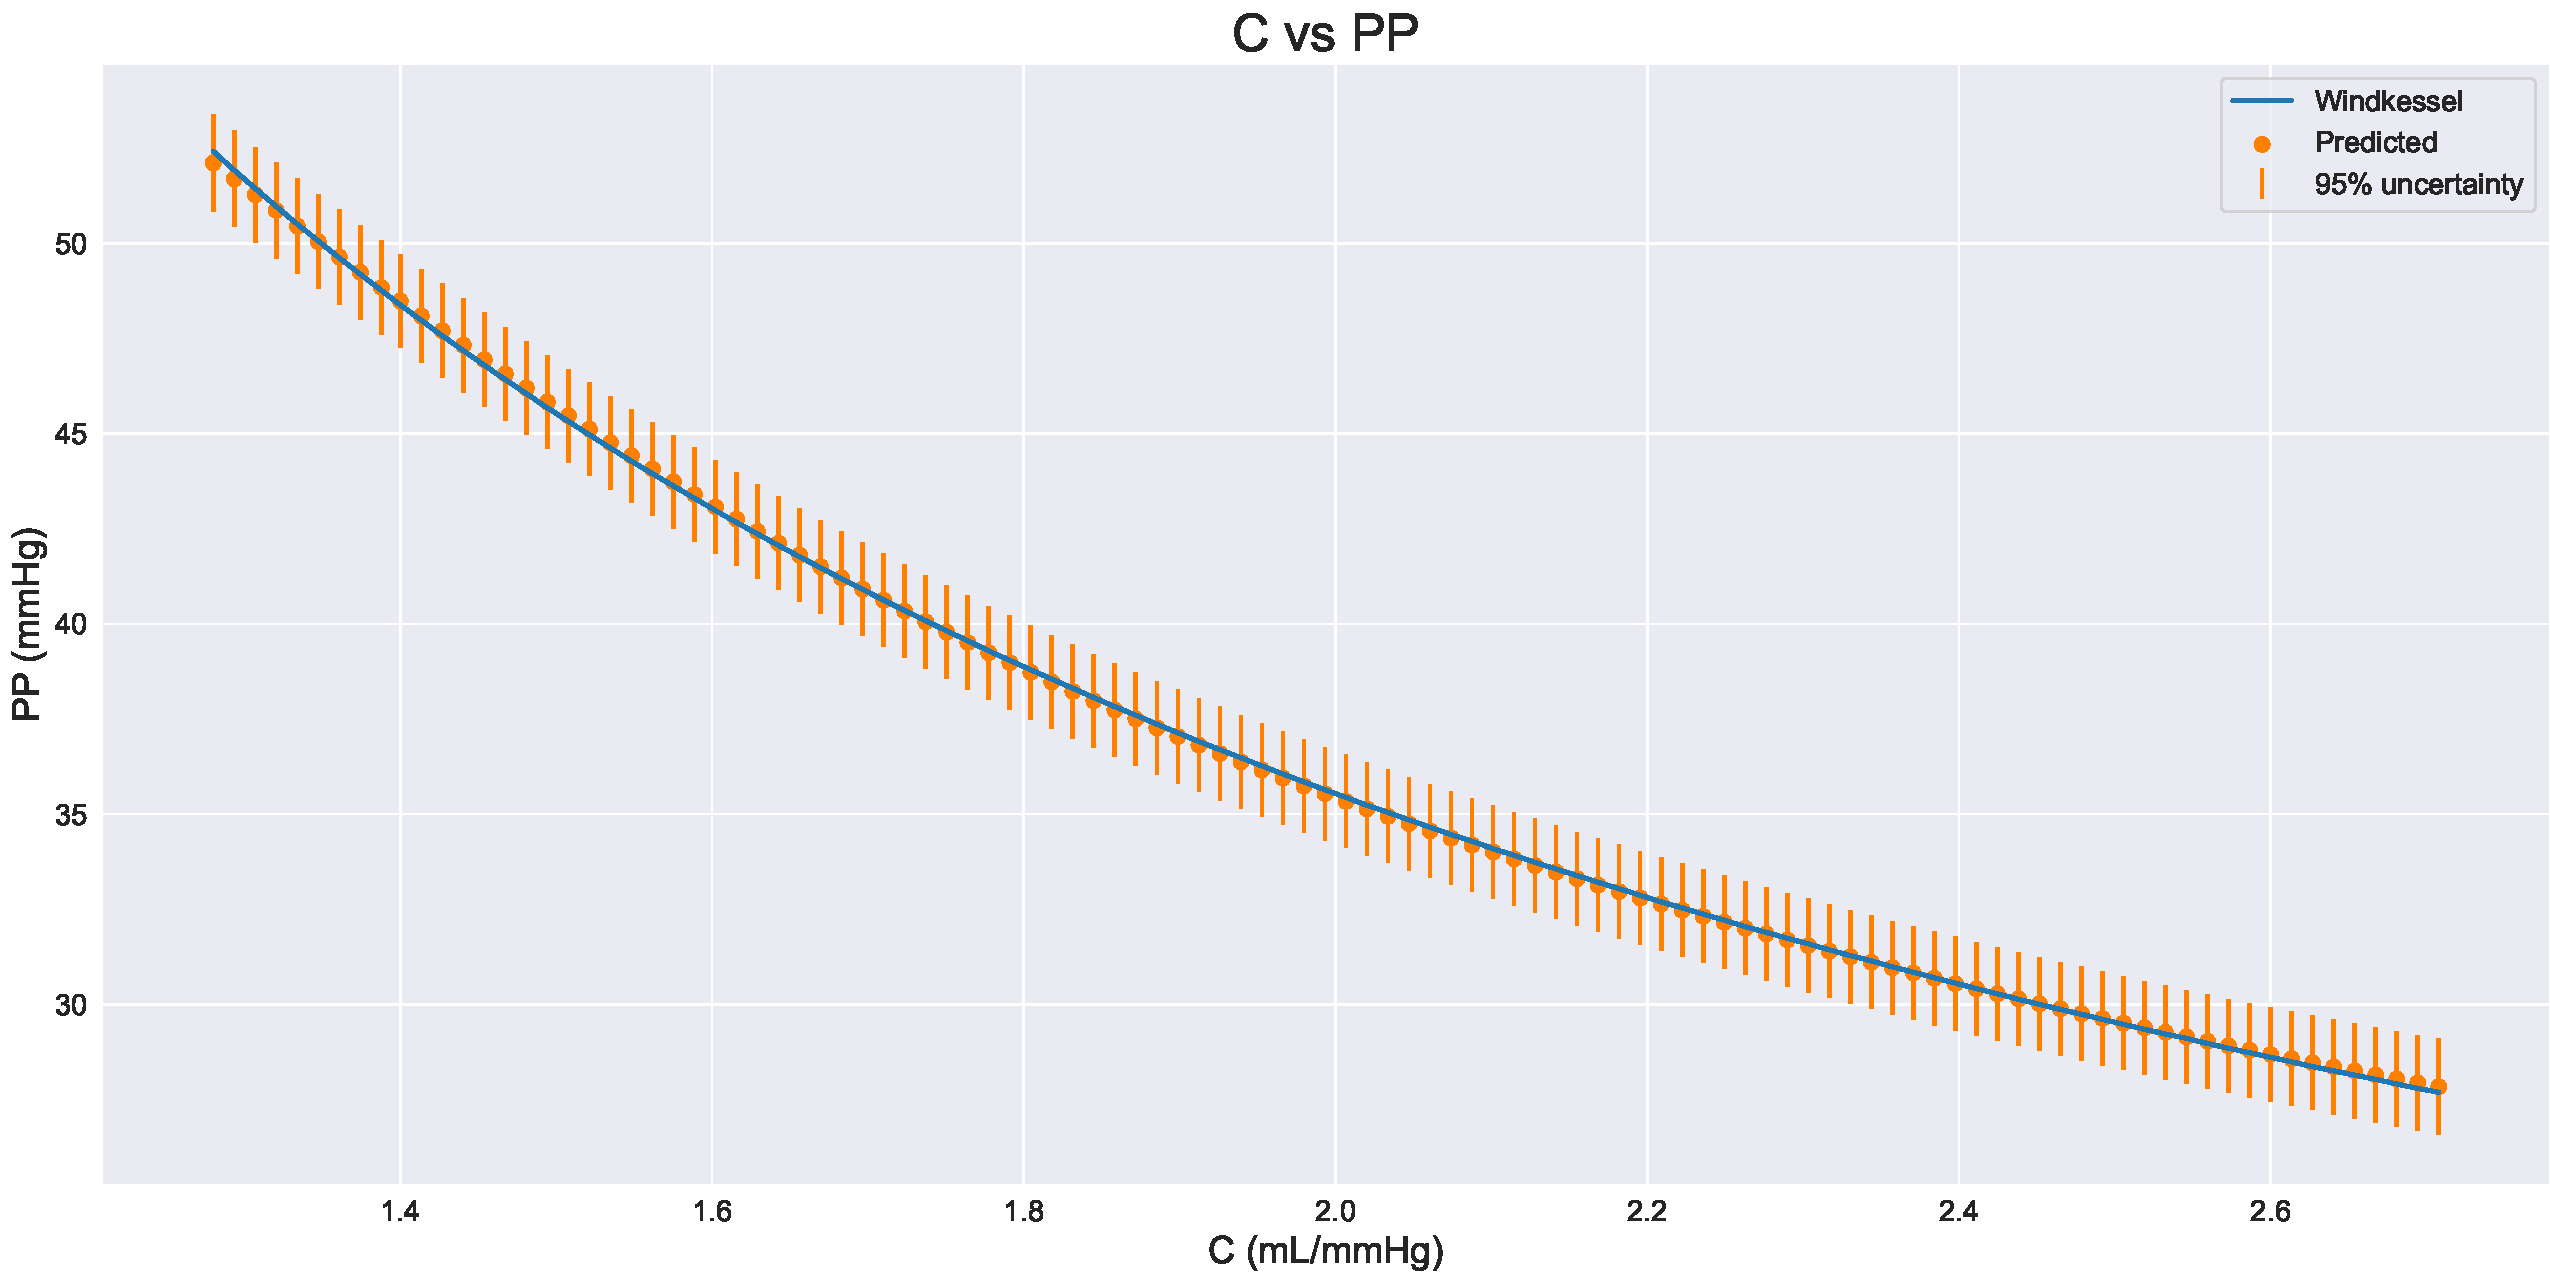
\includegraphics[width=1\textwidth]{images/Training (risultati)/PP/PP - C - full.pdf}
    \caption{Dipendenza di PP da $C$ sull'intervallo di training e due intervalli attigui.}
    \label{PP - C - full}
\end{figure}

\vspace{0.32cm}

\begin{figure}[!htb]
    \centering
    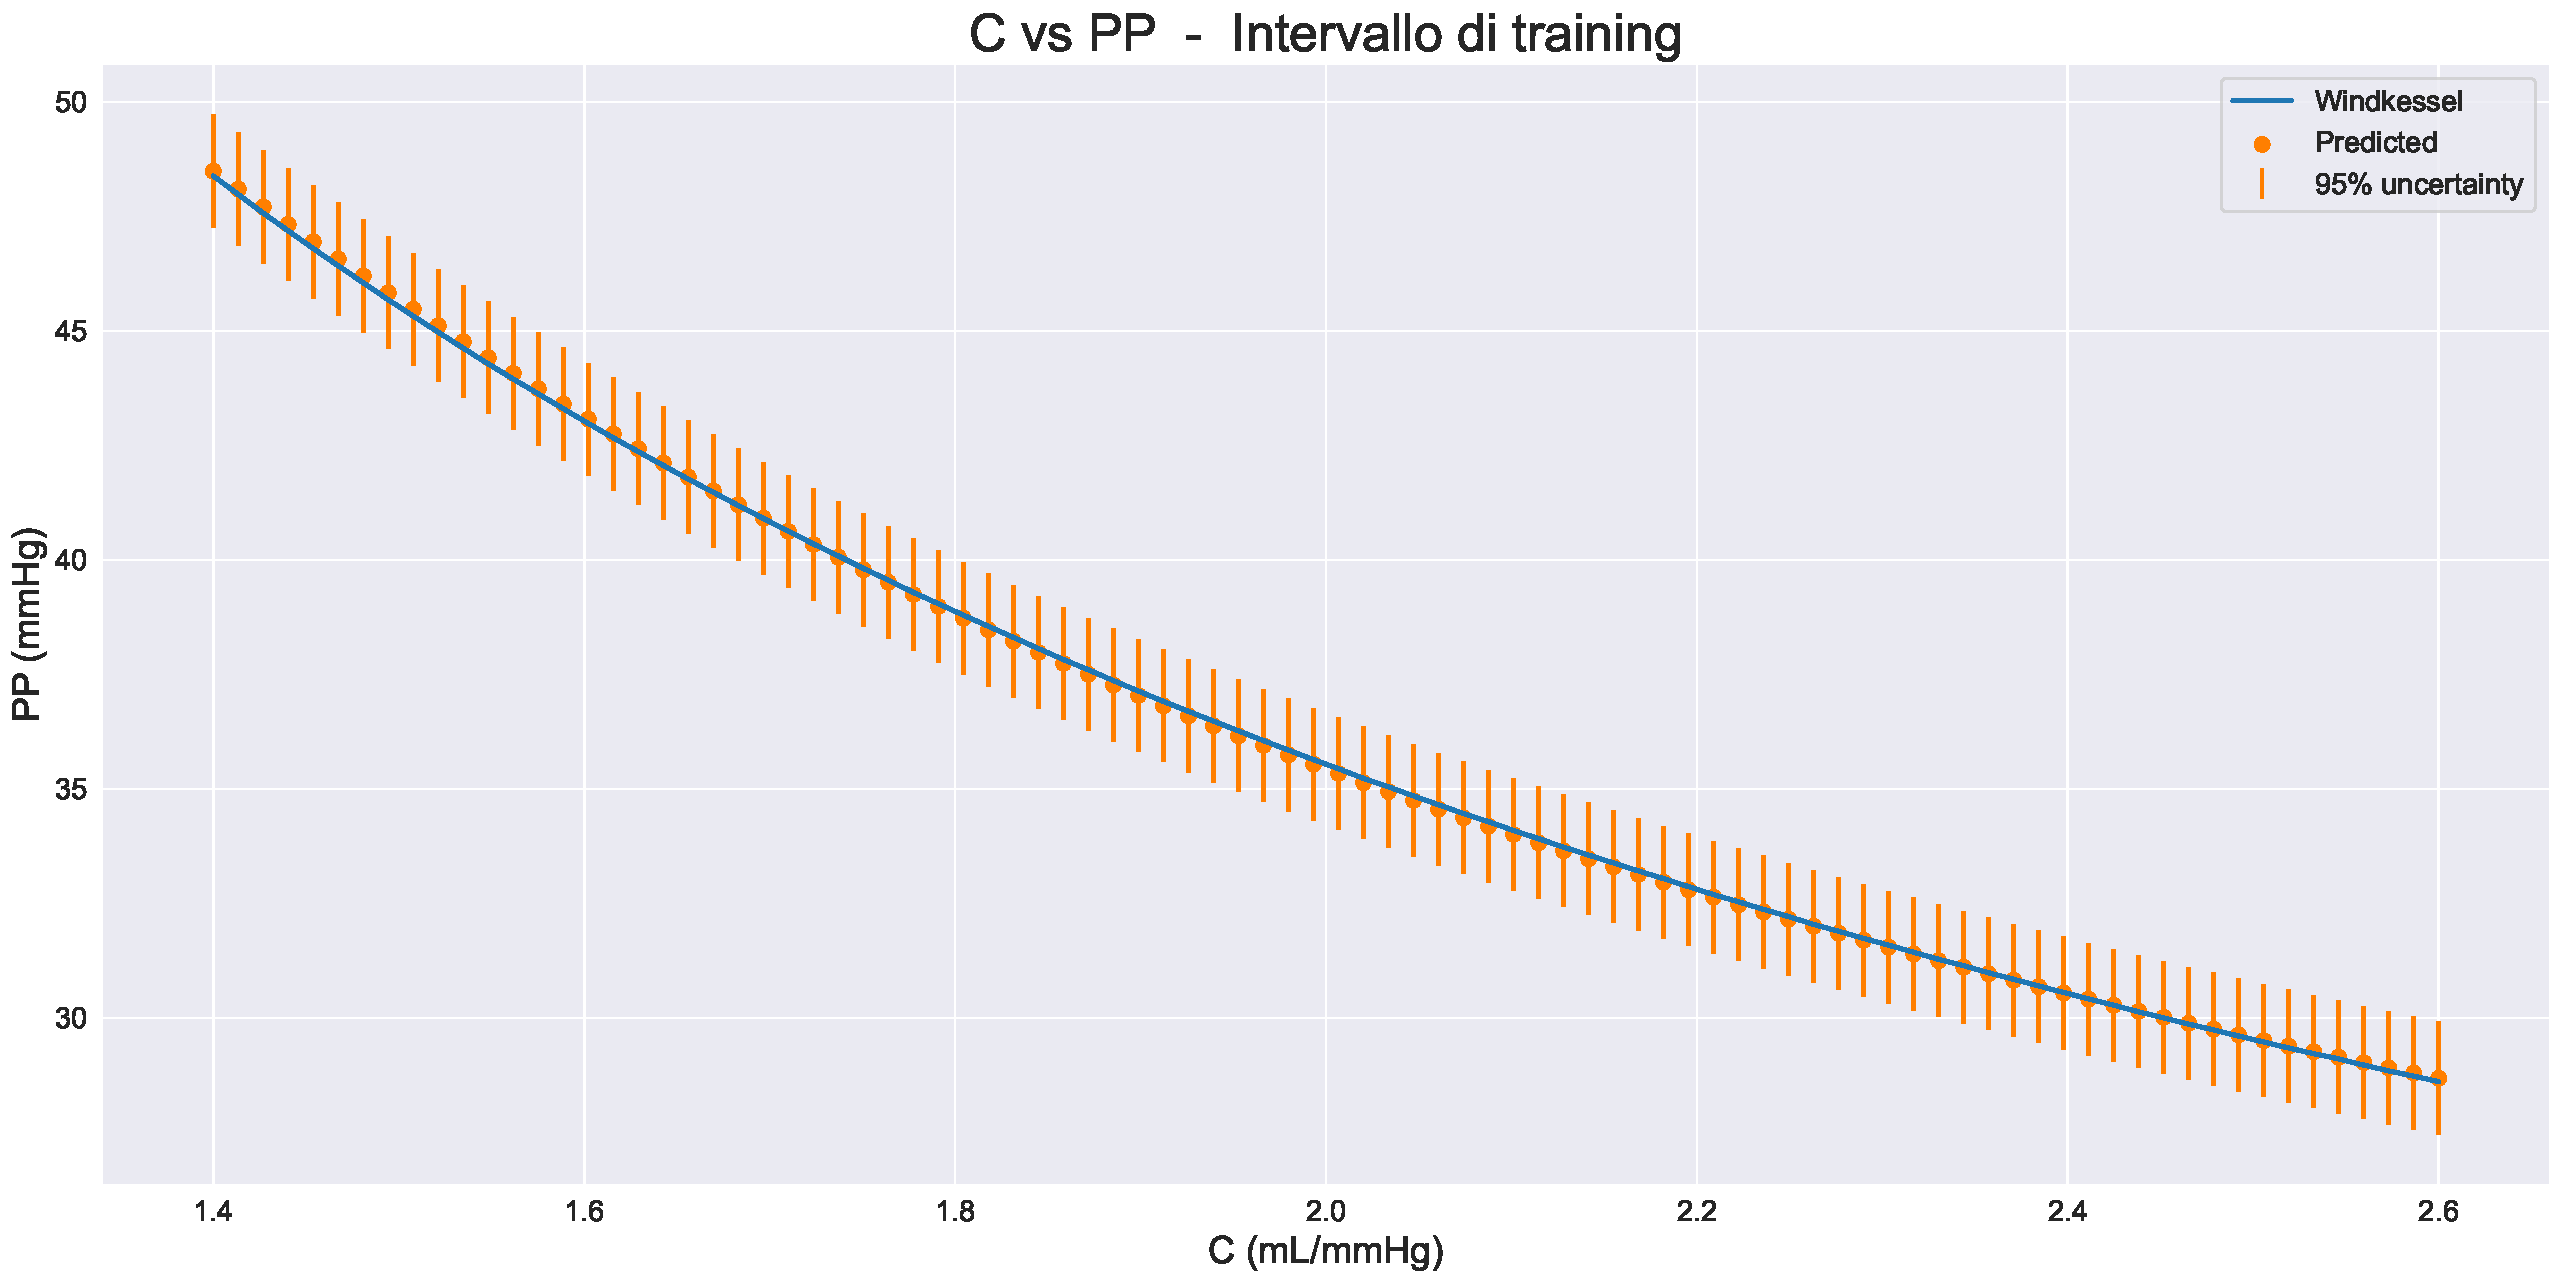
\includegraphics[width=1\textwidth]{images/Training (risultati)/PP/PP - C - training.pdf}
    \caption{Dipendenza di PP da $C$ sull'intervallo di training.}
    \label{PP - C - training}
\end{figure}

\begin{figure}
    \centering
    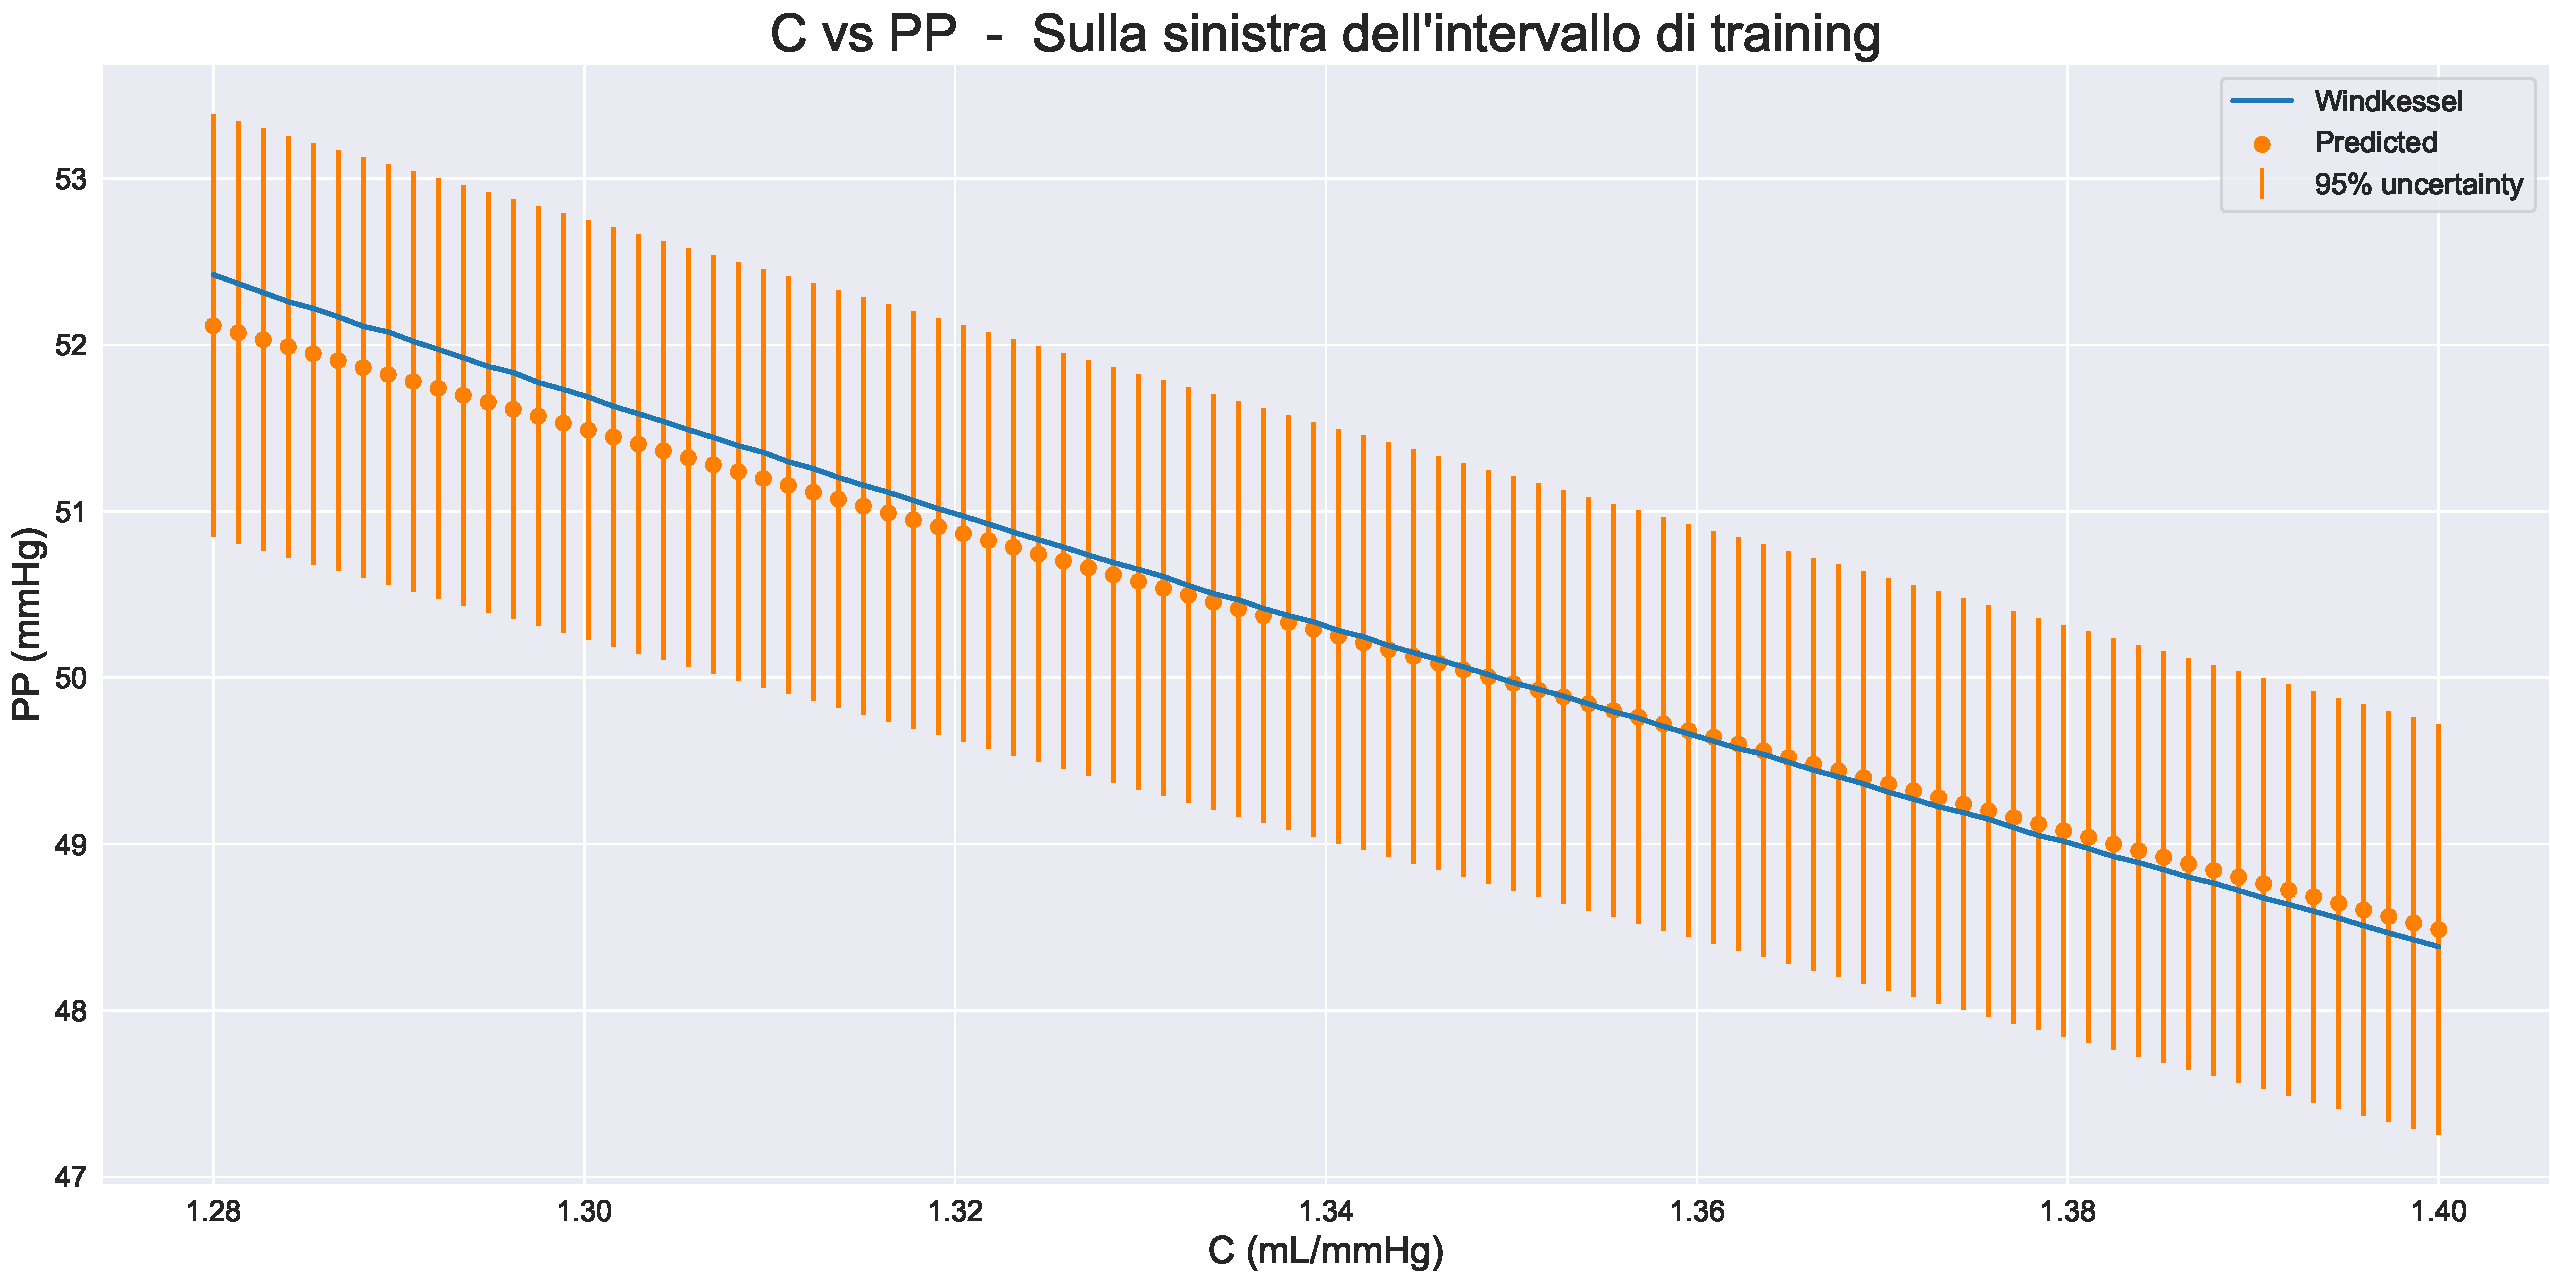
\includegraphics[width=1\textwidth]{images/Training (risultati)/PP/PP - C - sx.pdf}
    \caption{Dipendenza di PP da $C$ sull'intervallo attiguo a sinistra dell'intervallo di training.}
    \label{PP - C - sx}
\end{figure}



\begin{figure}
    \centering
    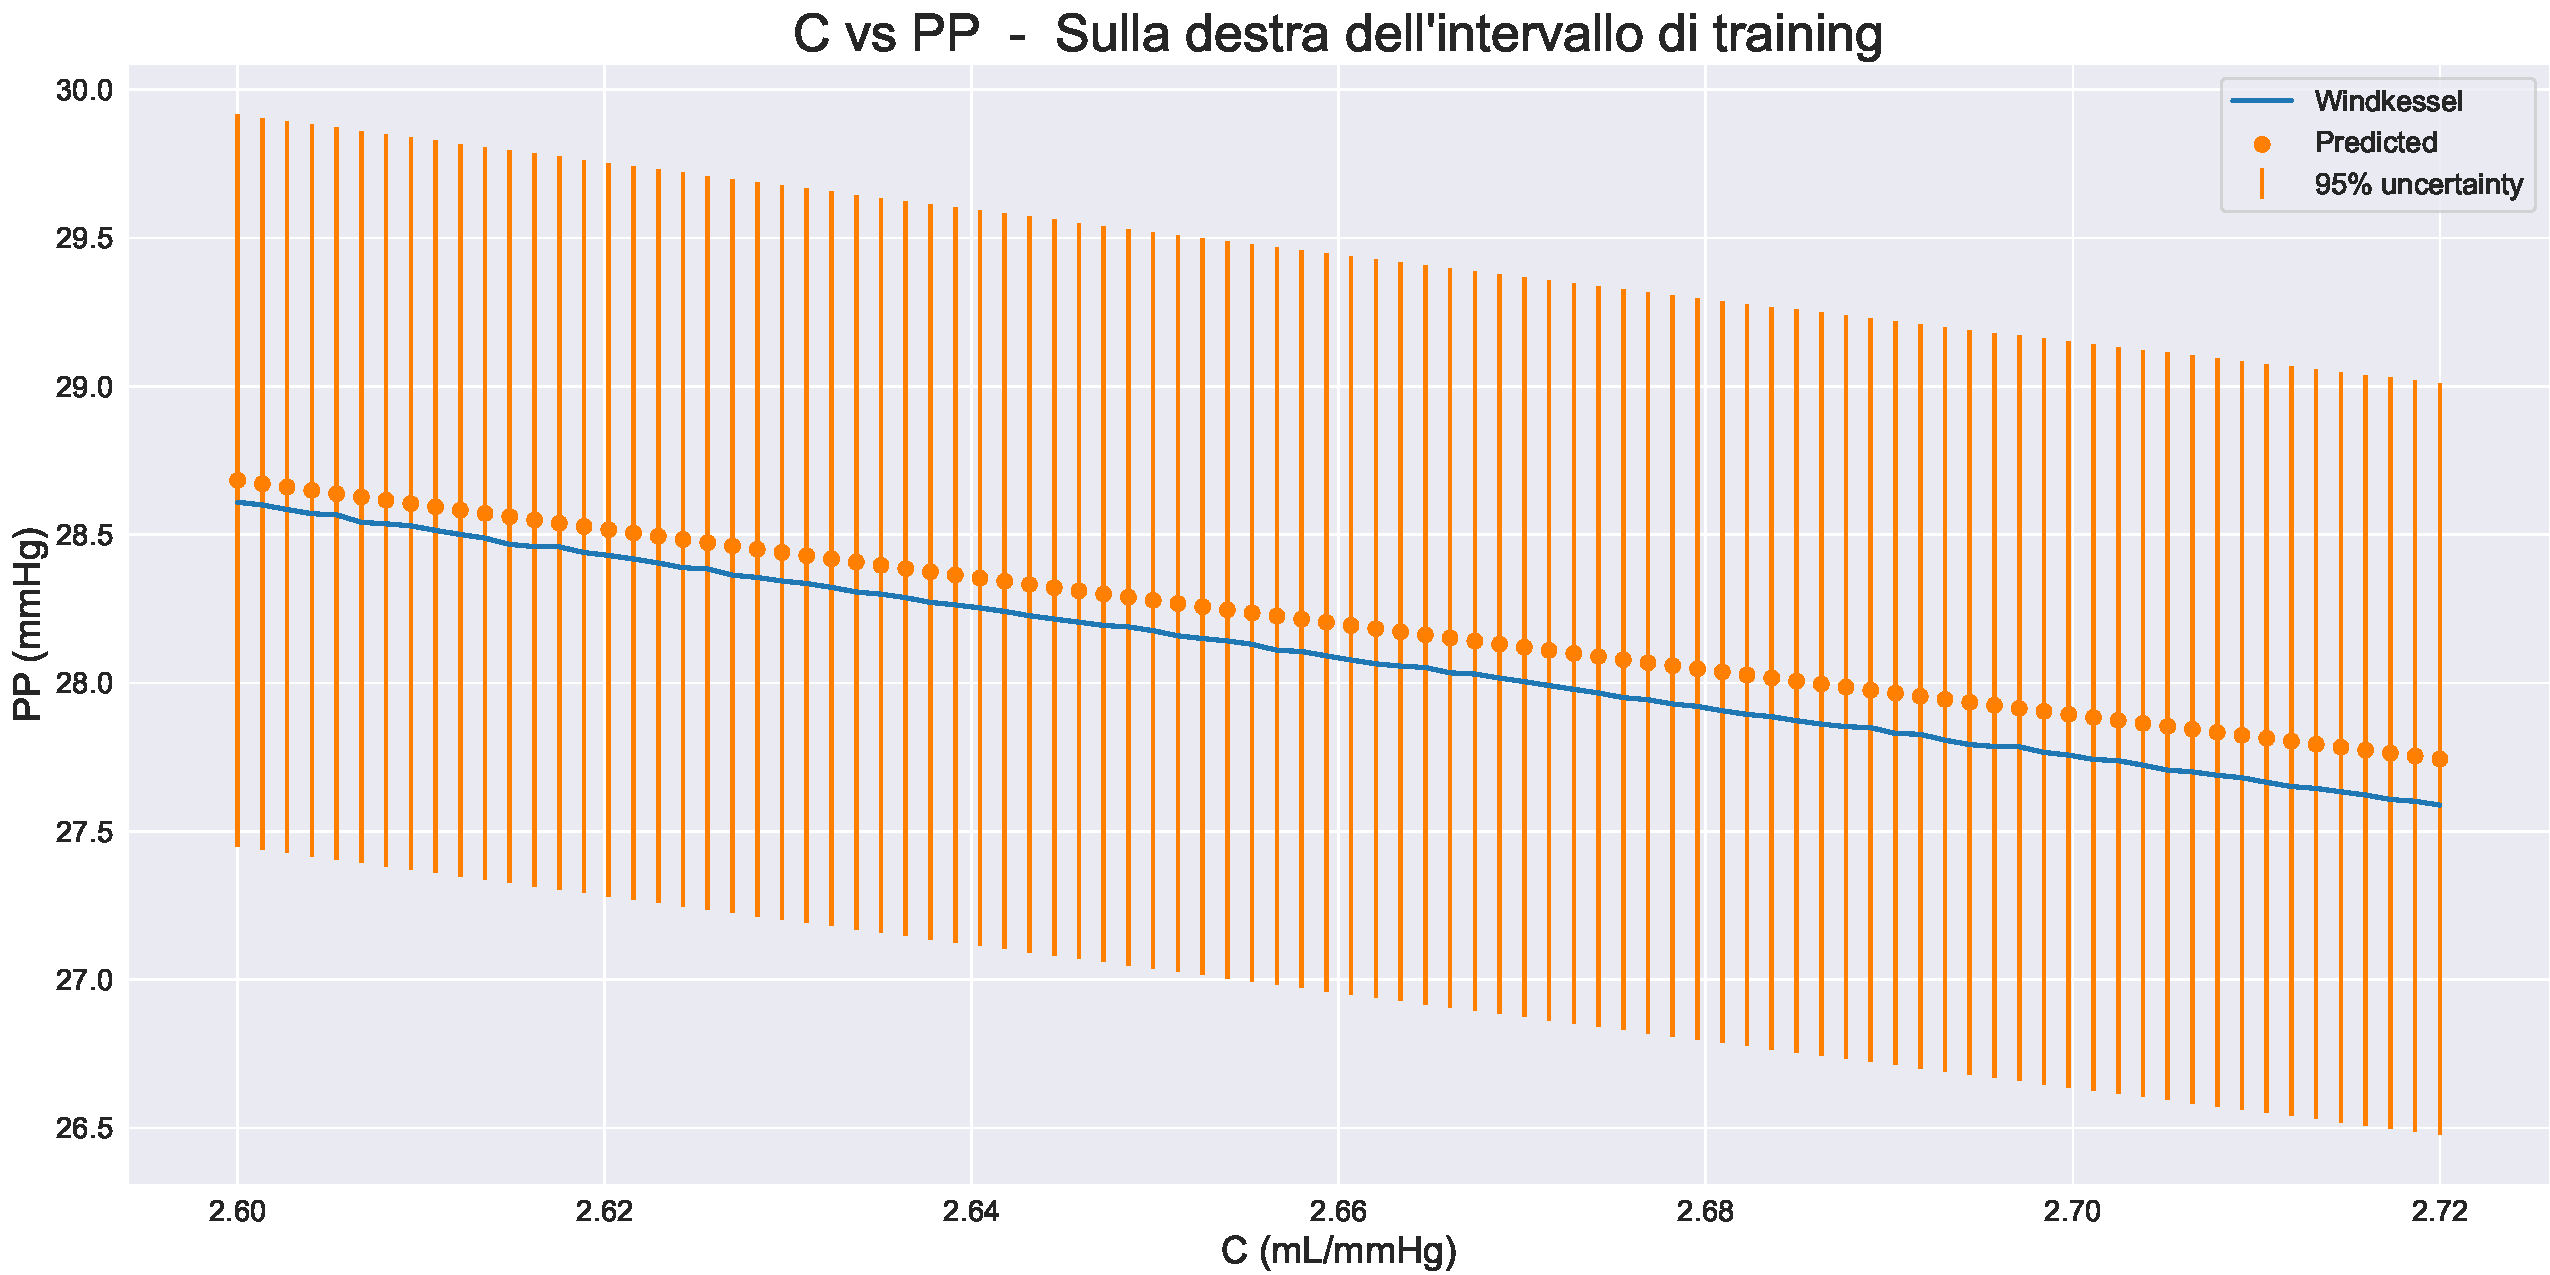
\includegraphics[width=1\textwidth]{images/Training (risultati)/PP/PP - C - dx.pdf}
    \caption{Dipendenza di PP da $C$ sull'intervallo attiguo a destra dell'intervallo di training.}
    \label{PP - C - dx}
\end{figure}




\newpage
% **********
% PP - R1
% **********
\subsubsection{Dipendenza da $R_1$}
Il risultato complessivo è mostrato in figura \ref{PP - R1 - full}, il risultato nel solo intervallo di training in \ref{PP - R1 - training}, il risultato nei singoli intervalli attigui in \ref{PP - R1 - sx} e \ref{PP - R1 - dx}.

\vspace{1cm}

\begin{figure}[!htb]
    \centering
    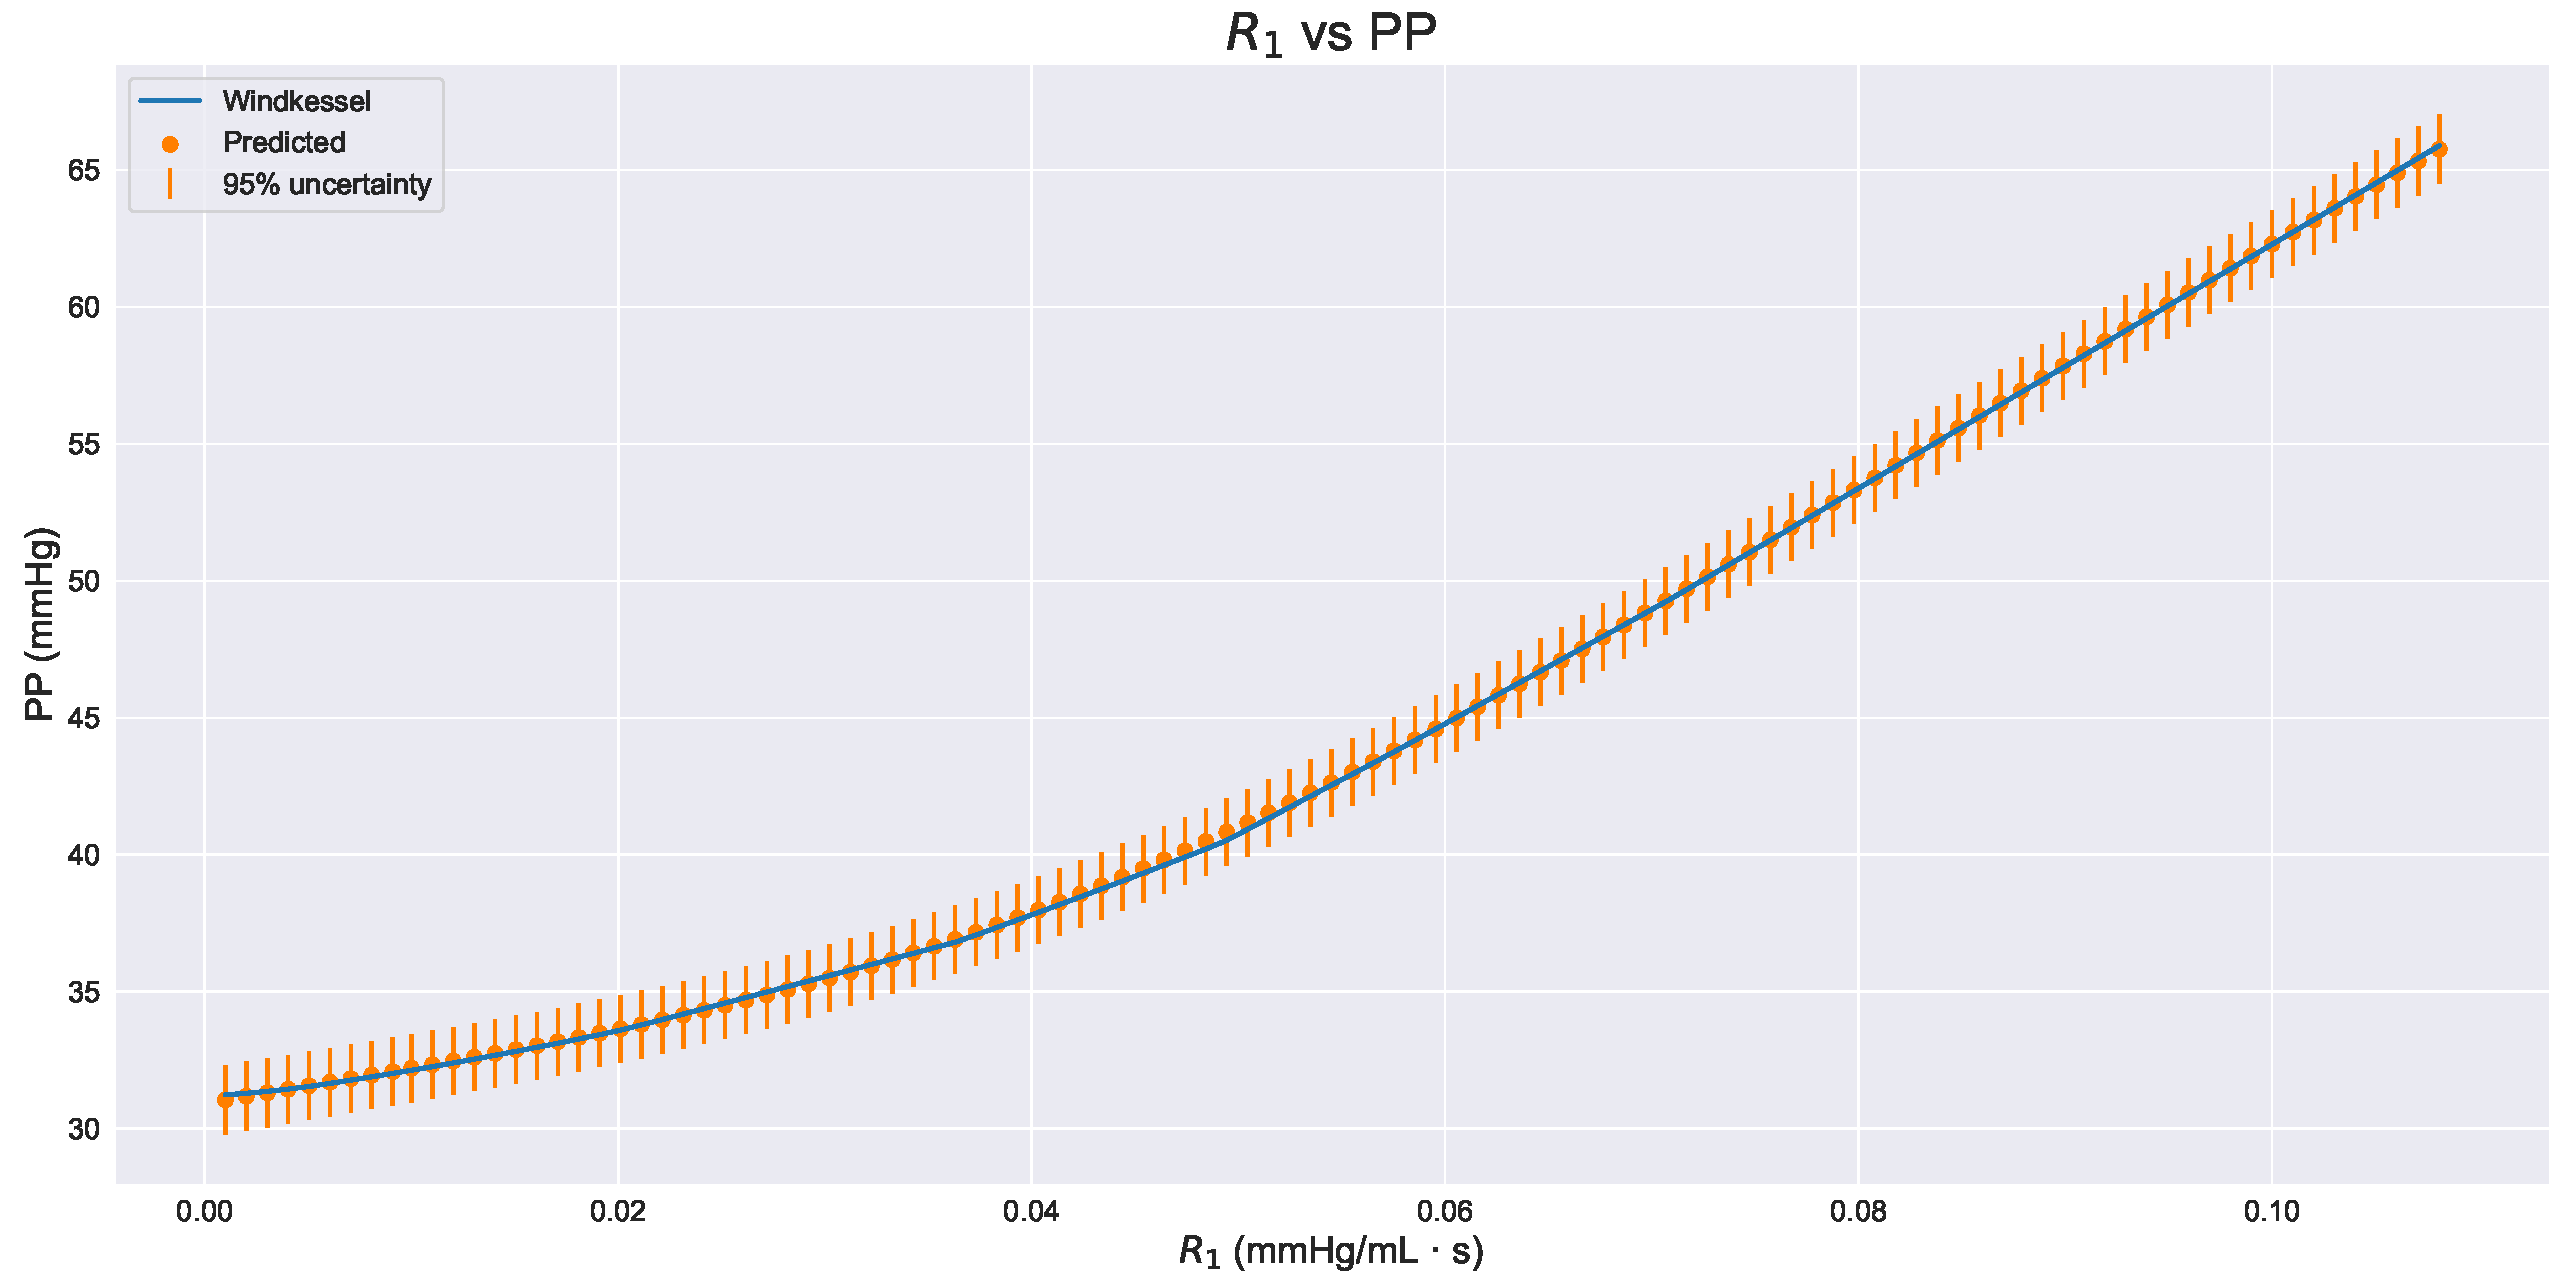
\includegraphics[width=1\textwidth]{images/Training (risultati)/PP/PP - R1 - full.pdf}
    \caption{Dipendenza di PP da $R1$ sull'intervallo di training e due intervalli attigui.}
    \label{PP - R1 - full}
\end{figure}

\vspace{0.32cm}

\begin{figure}[!htb]
    \centering
    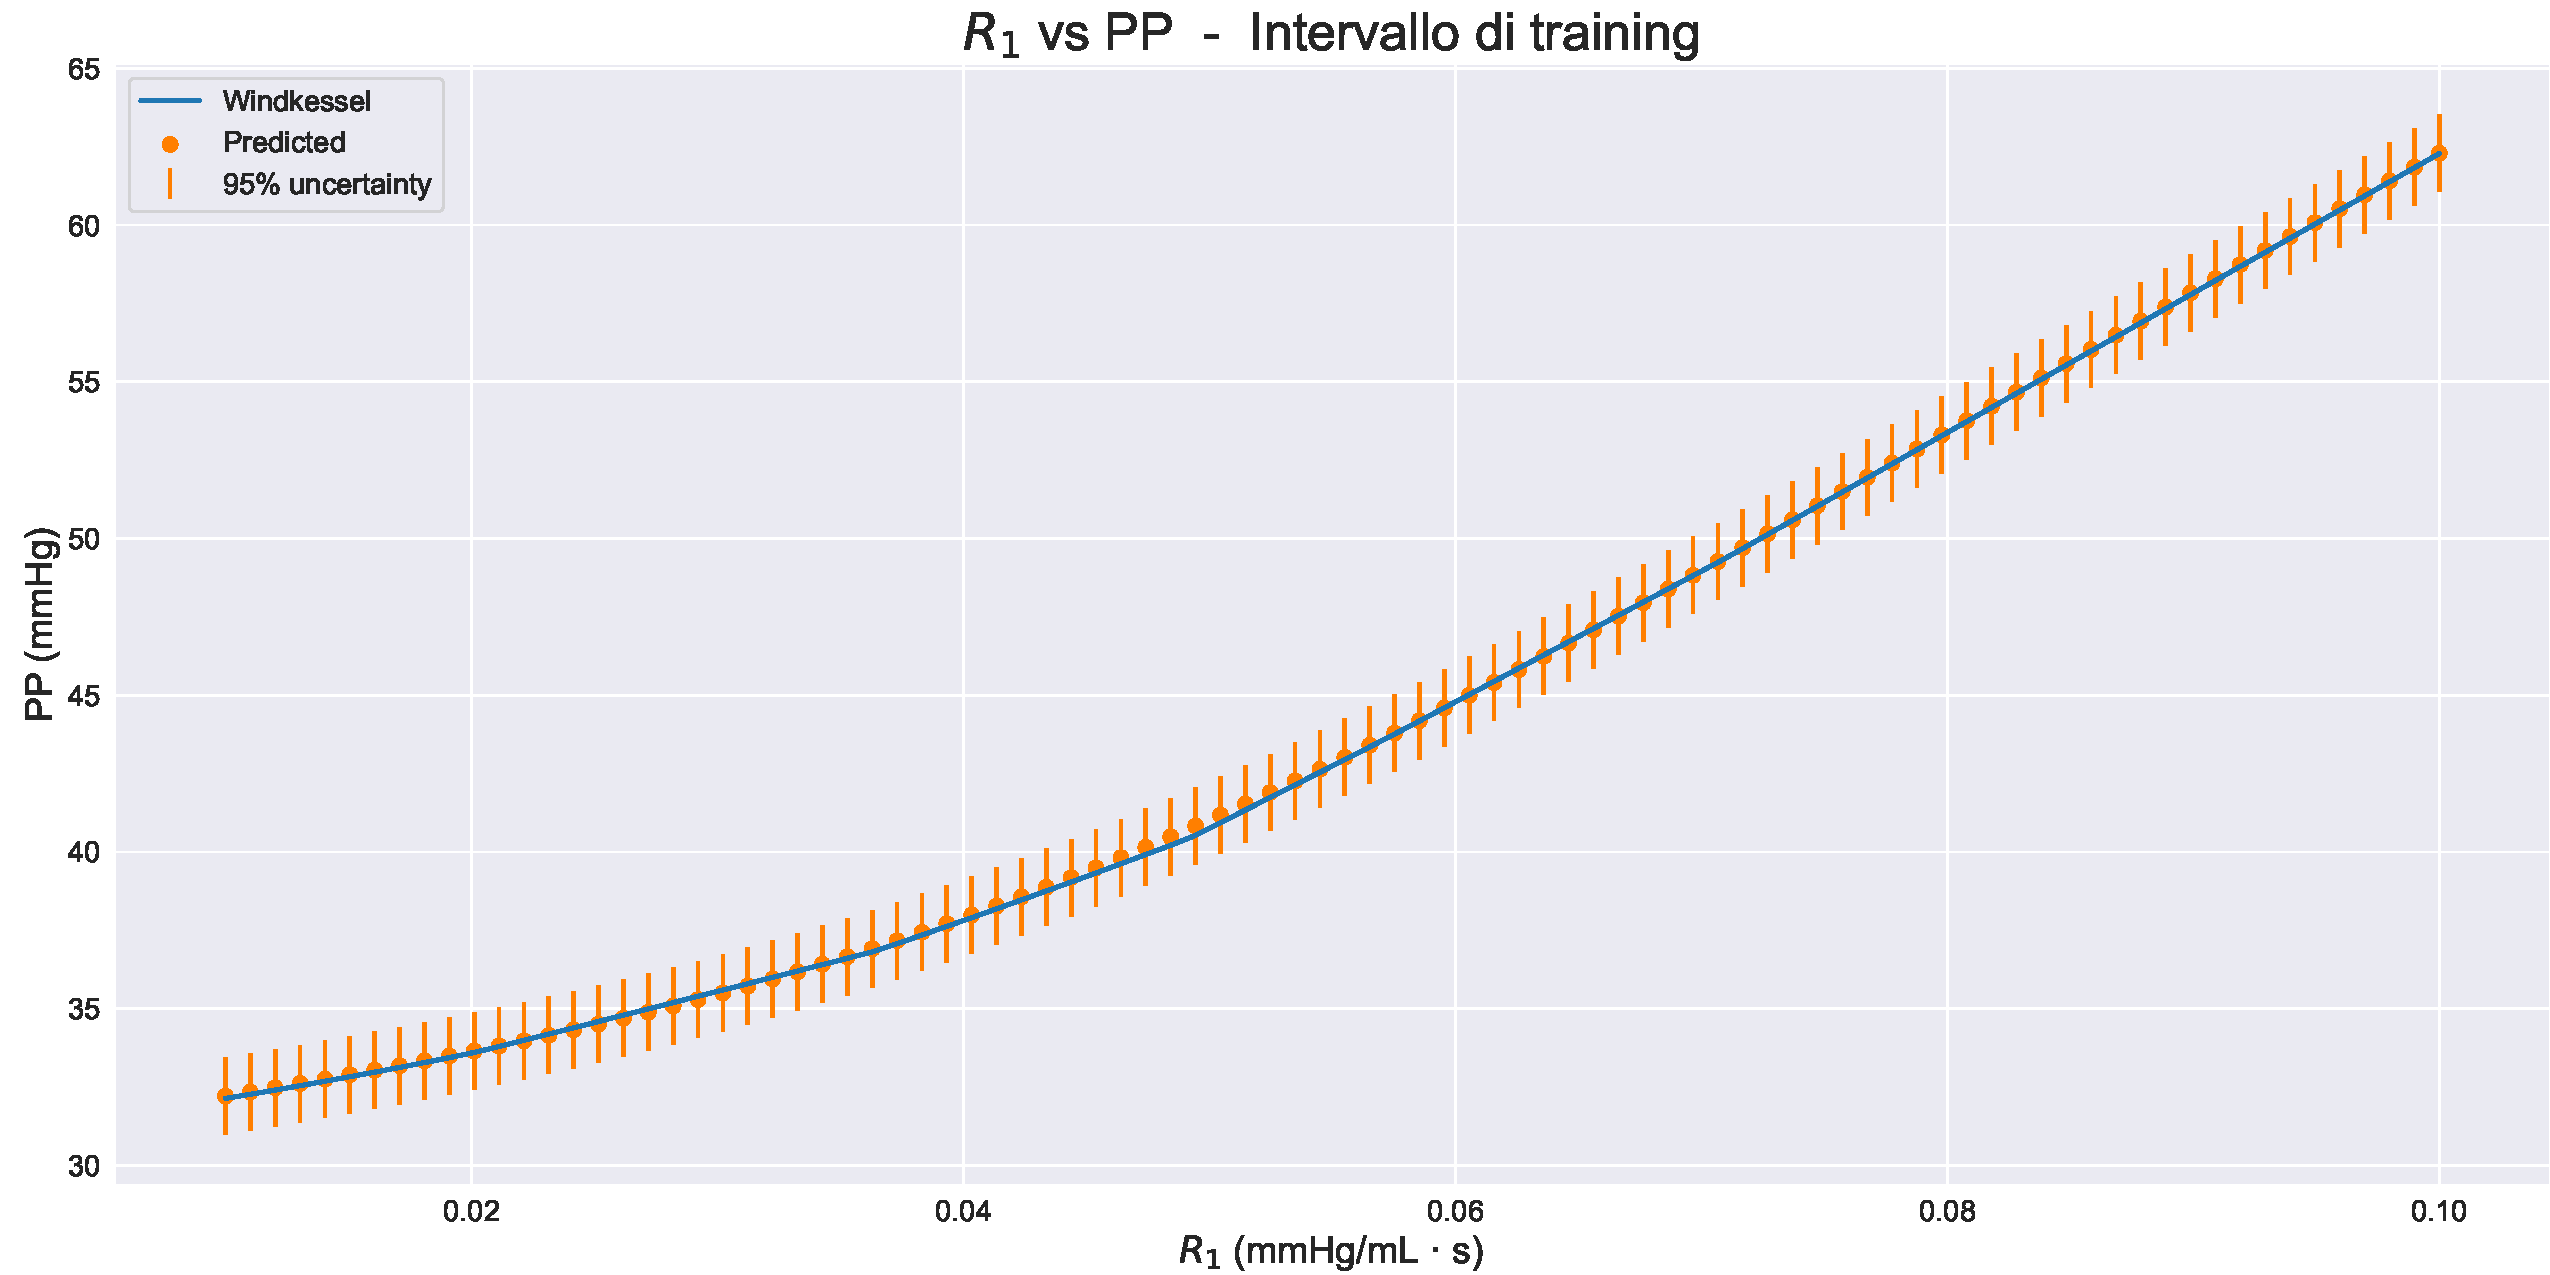
\includegraphics[width=1\textwidth]{images/Training (risultati)/PP/PP - R1 - training.pdf}
    \caption{Dipendenza di PP da $R1$ sull'intervallo di training.}
    \label{PP - R1 - training}
\end{figure}

\begin{figure}
    \centering
    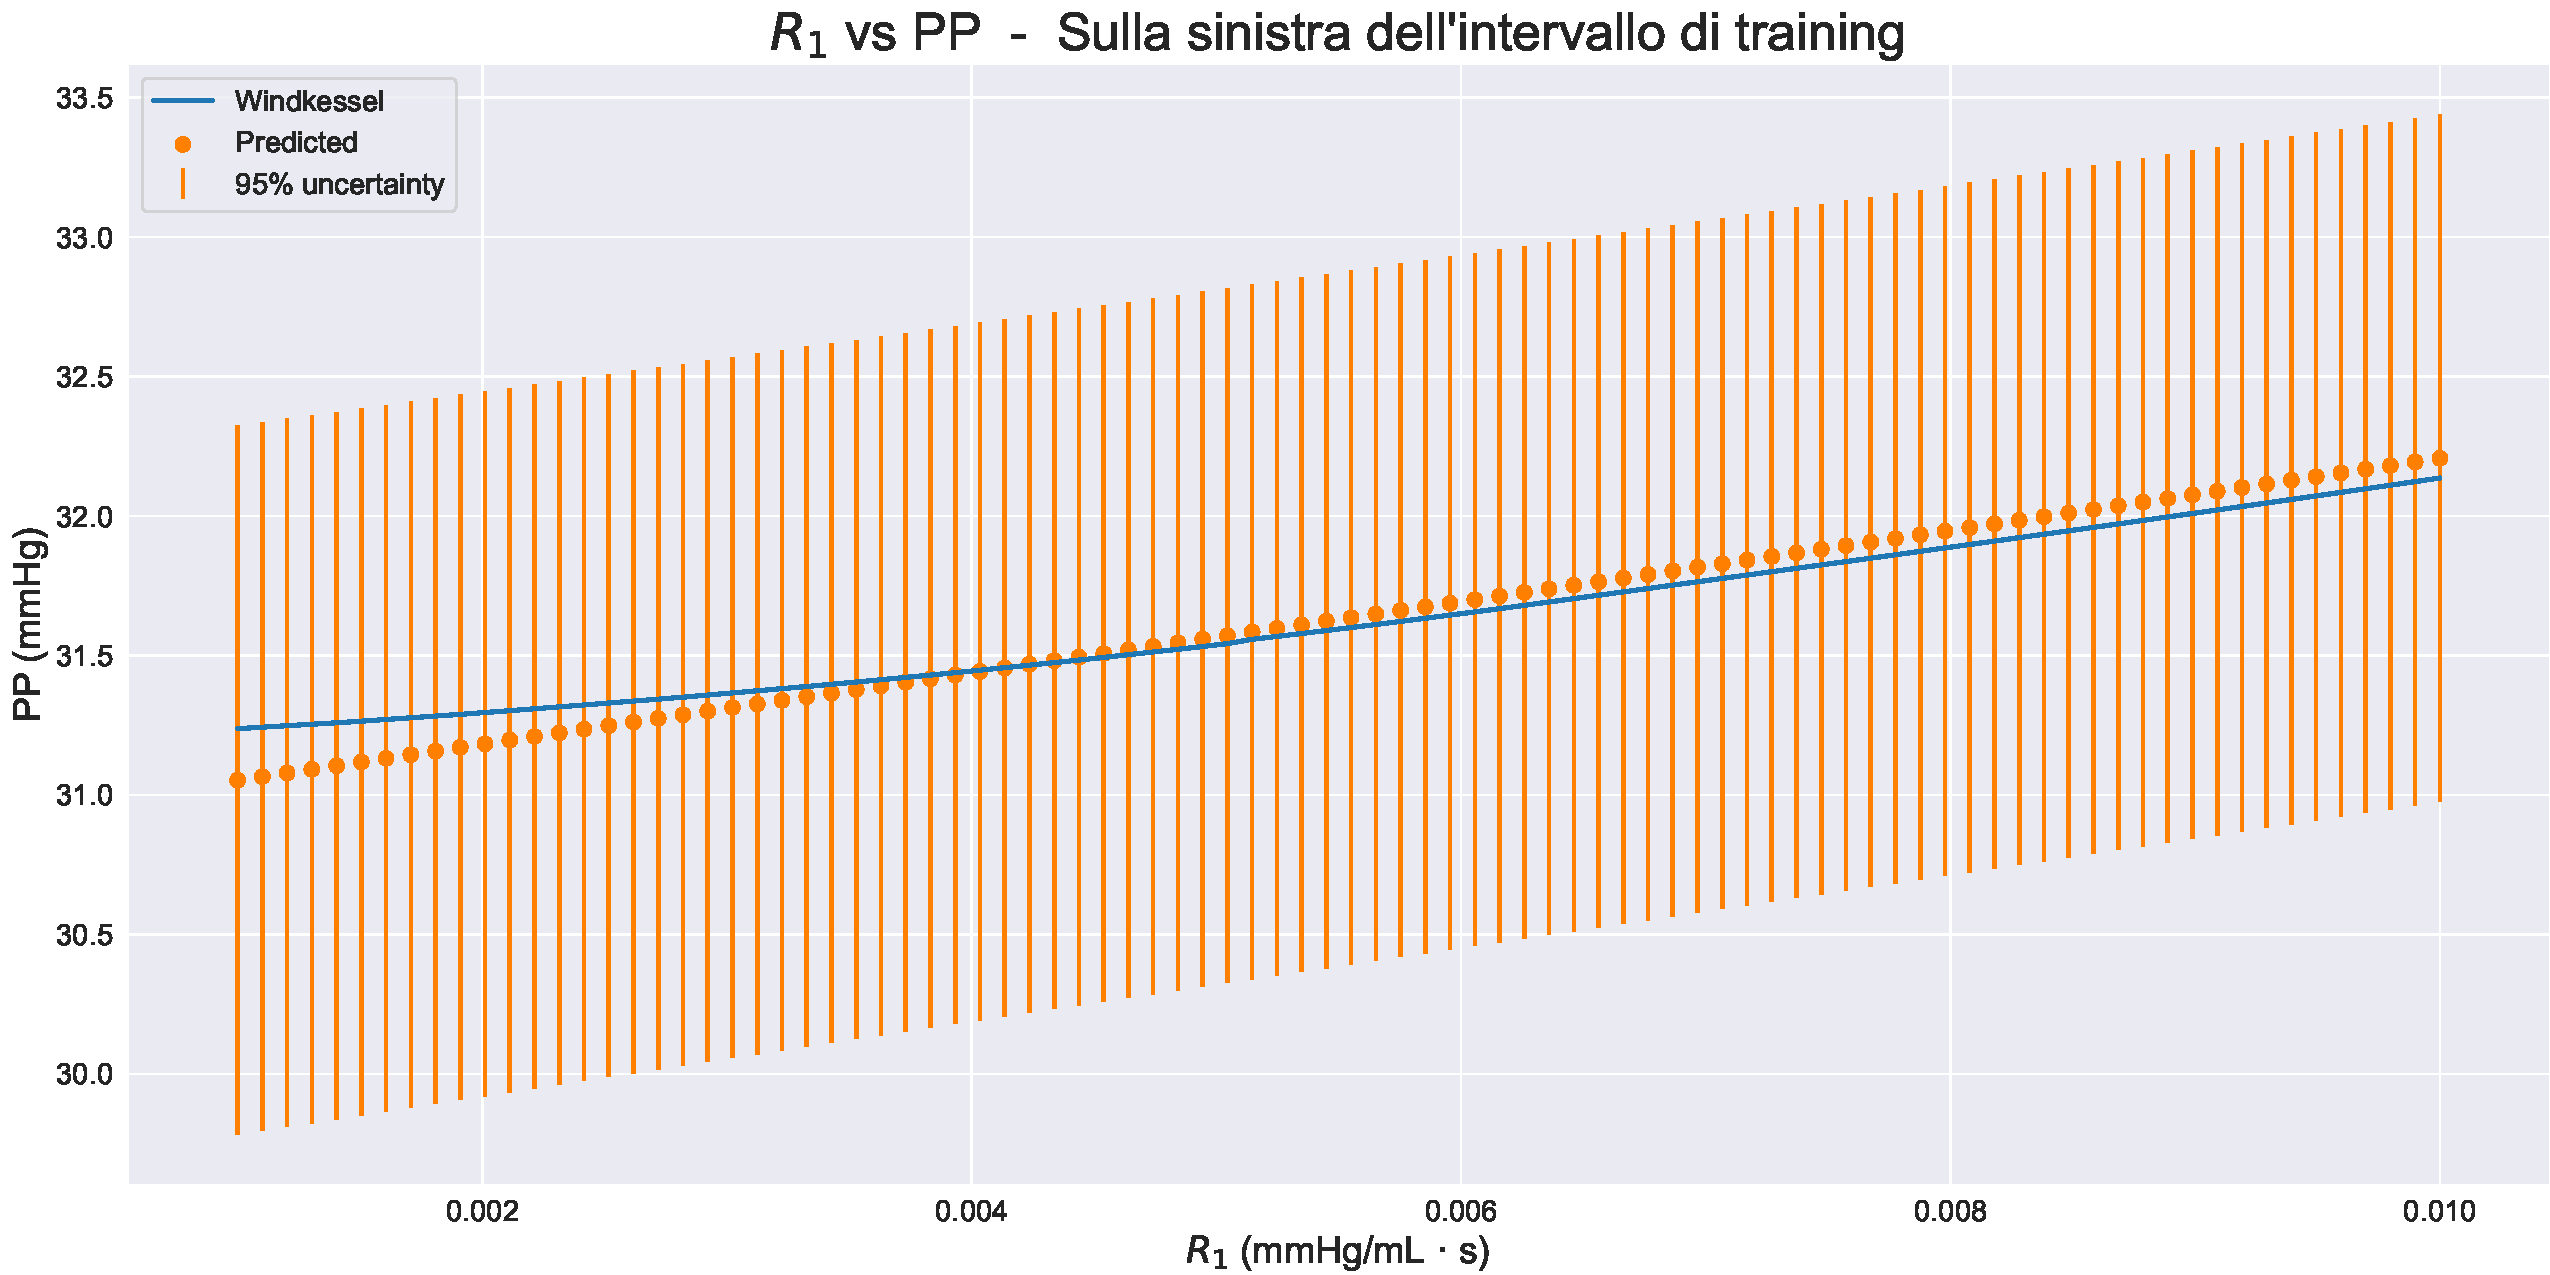
\includegraphics[width=1\textwidth]{images/Training (risultati)/PP/PP - R1 - sx.pdf}
    \caption{Dipendenza di PP da $R1$ sull'intervallo attiguo a sinistra dell'intervallo di training.}
    \label{PP - R1 - sx}
\end{figure}



\begin{figure}
    \centering
    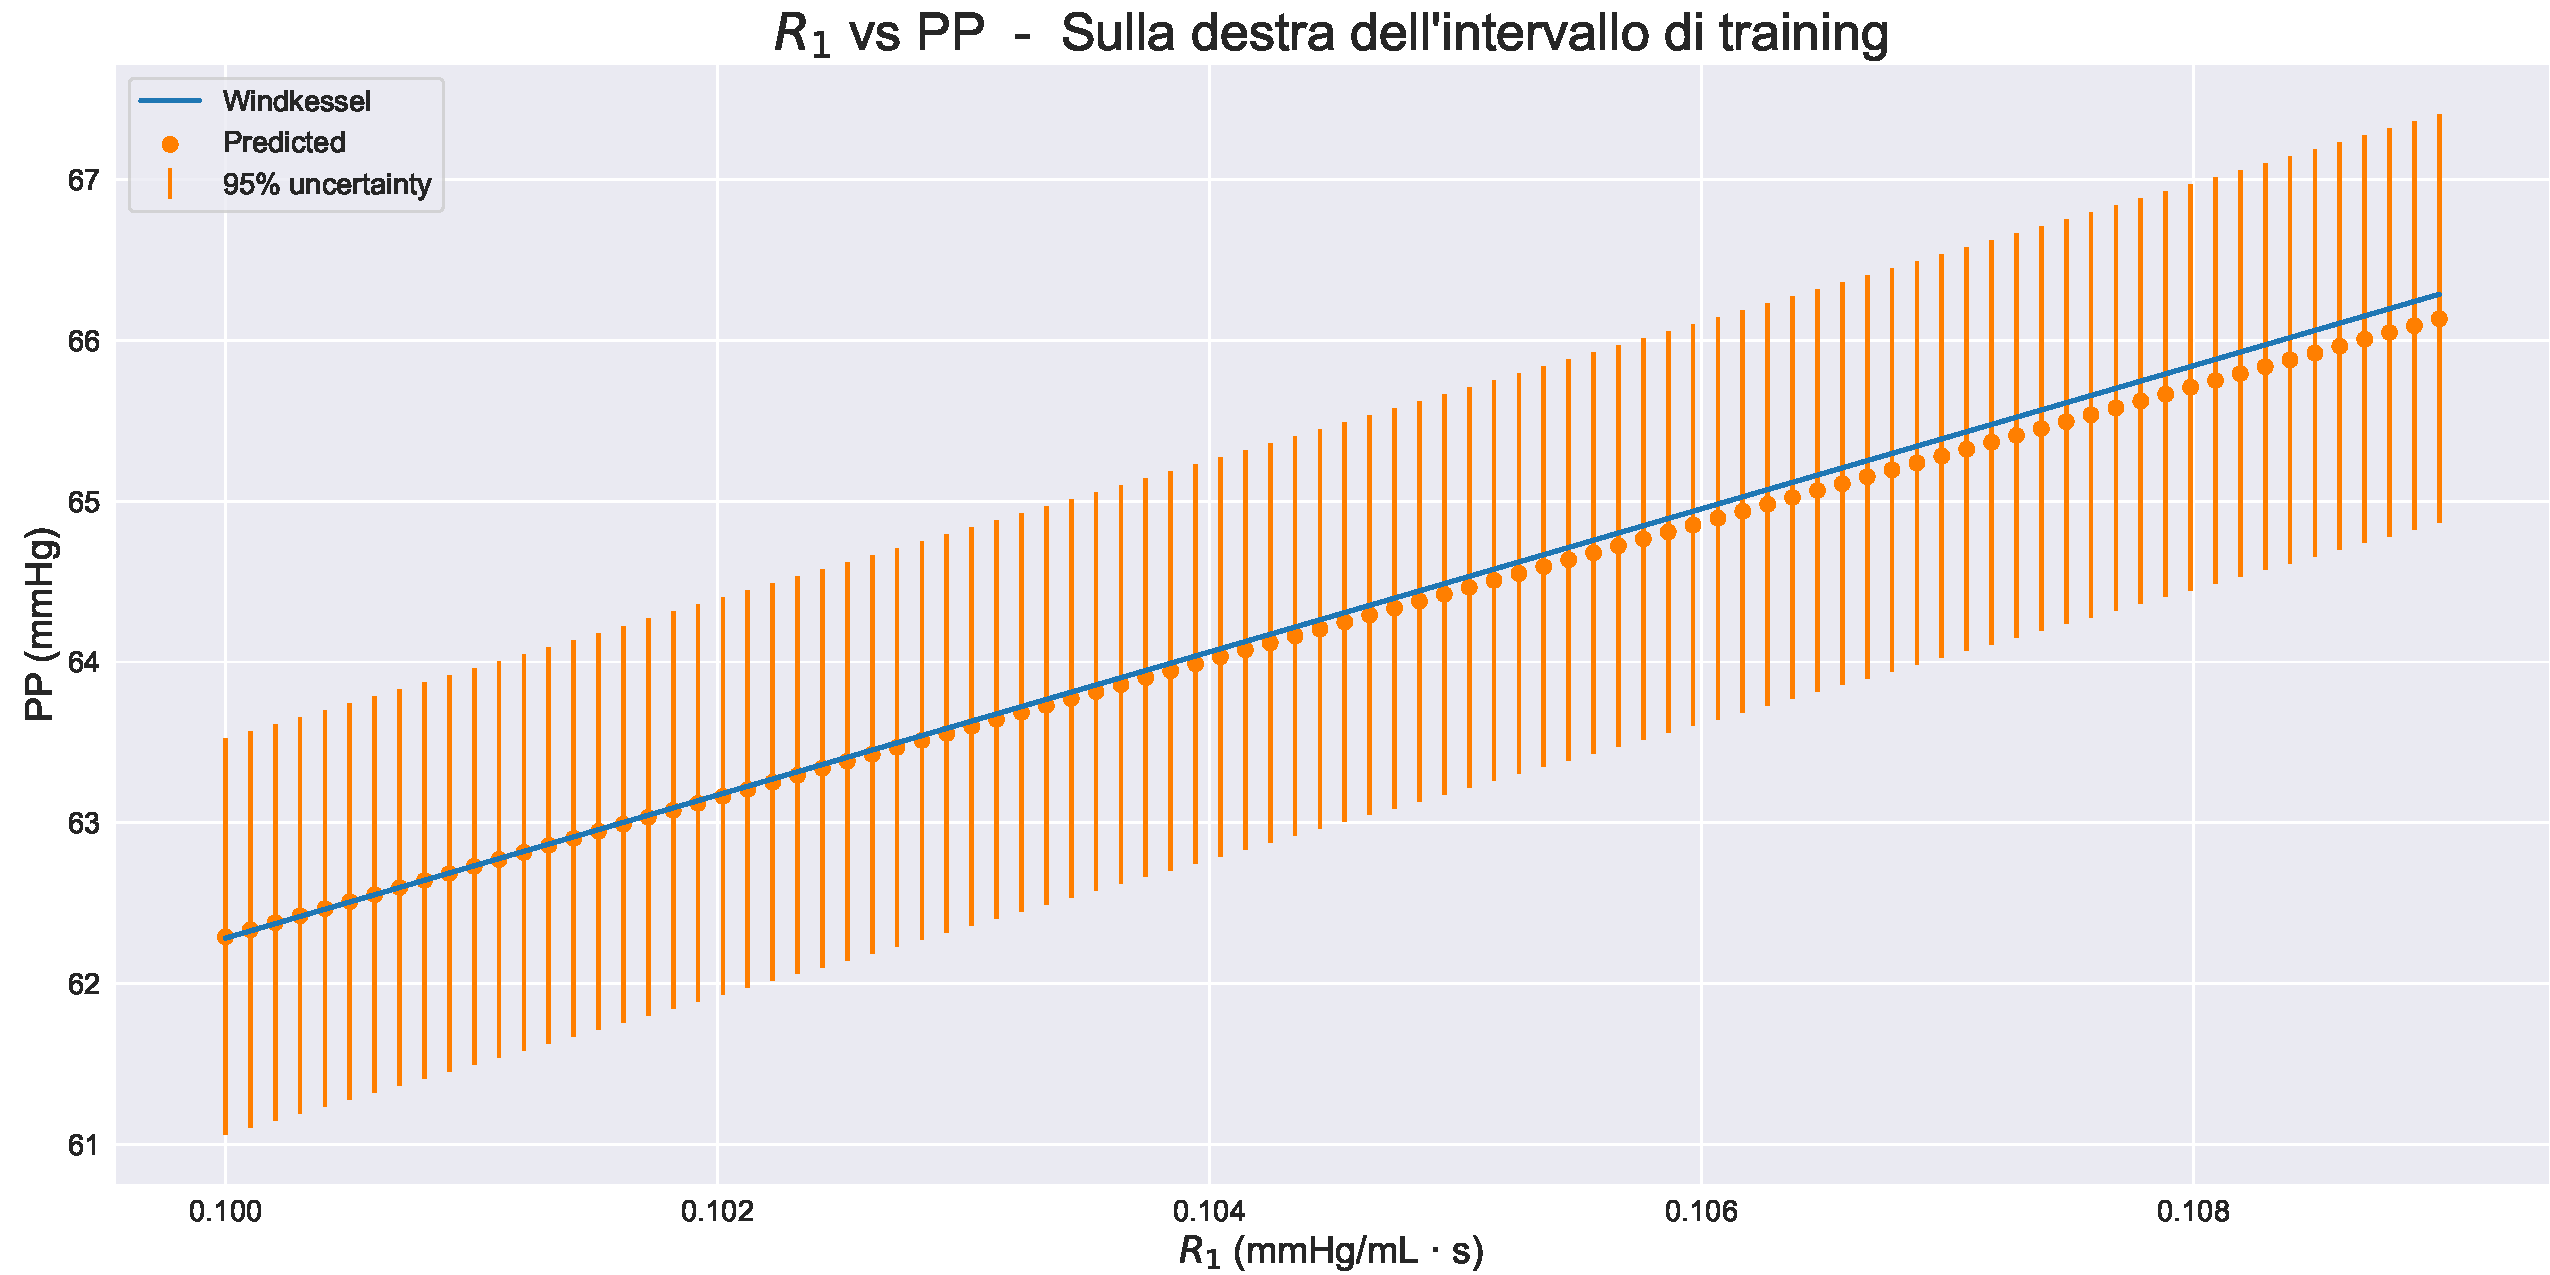
\includegraphics[width=1\textwidth]{images/Training (risultati)/PP/PP - R1 - dx.pdf}
    \caption{Dipendenza di PP da $R1$ sull'intervallo attiguo a destra dell'intervallo di training.}
    \label{PP - R1 - dx}
\end{figure}

\newpage


% **********
% PP - R2
% **********
\subsubsection{Dipendenza da $R_2$}
Il risultato complessivo è mostrato in figura \ref{PP - R2 - full}, il risultato nel solo intervallo di training in \ref{PP - R2 - training}, il risultato nei singoli intervalli attigui in \ref{PP - R2 - sx} e \ref{PP - R2 - dx}.

\vspace{0.9cm}

\begin{figure}[!htb]
    \centering
    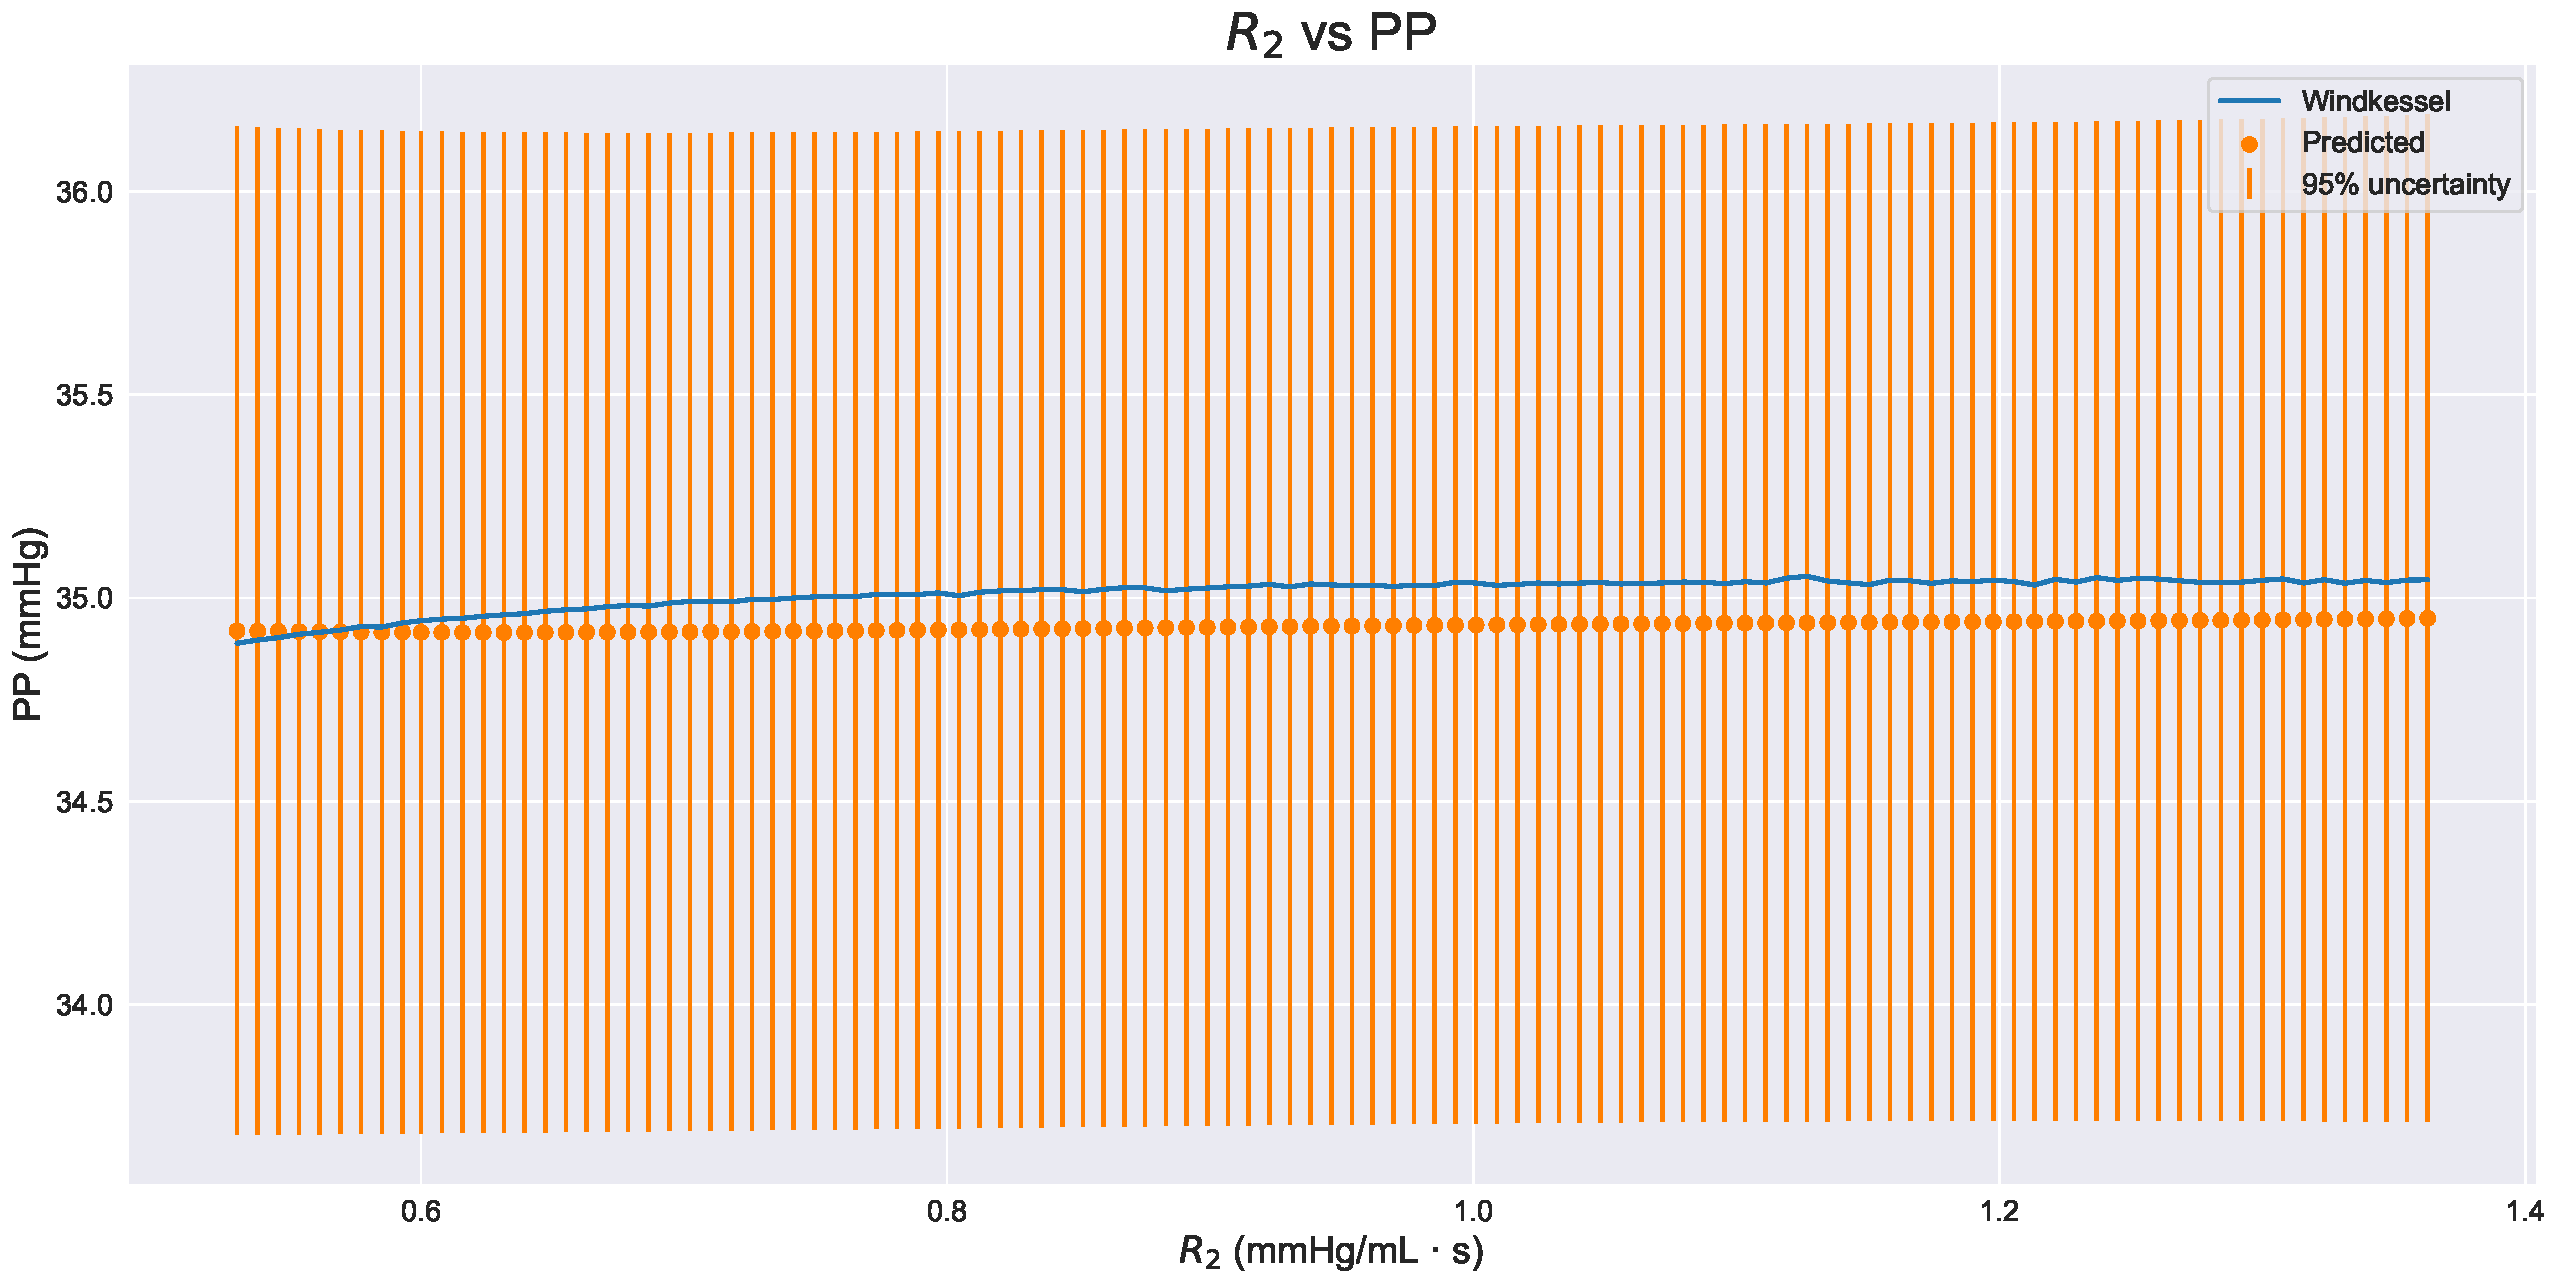
\includegraphics[width=1\textwidth]{images/Training (risultati)/PP/PP - R2 - full.pdf}
    \caption{Dipendenza di PP da $R2$ sull'intervallo di training e due intervalli attigui.}
    \label{PP - R2 - full}
\end{figure}

\vspace{0.32cm}

\begin{figure}[!htb]
    \centering
    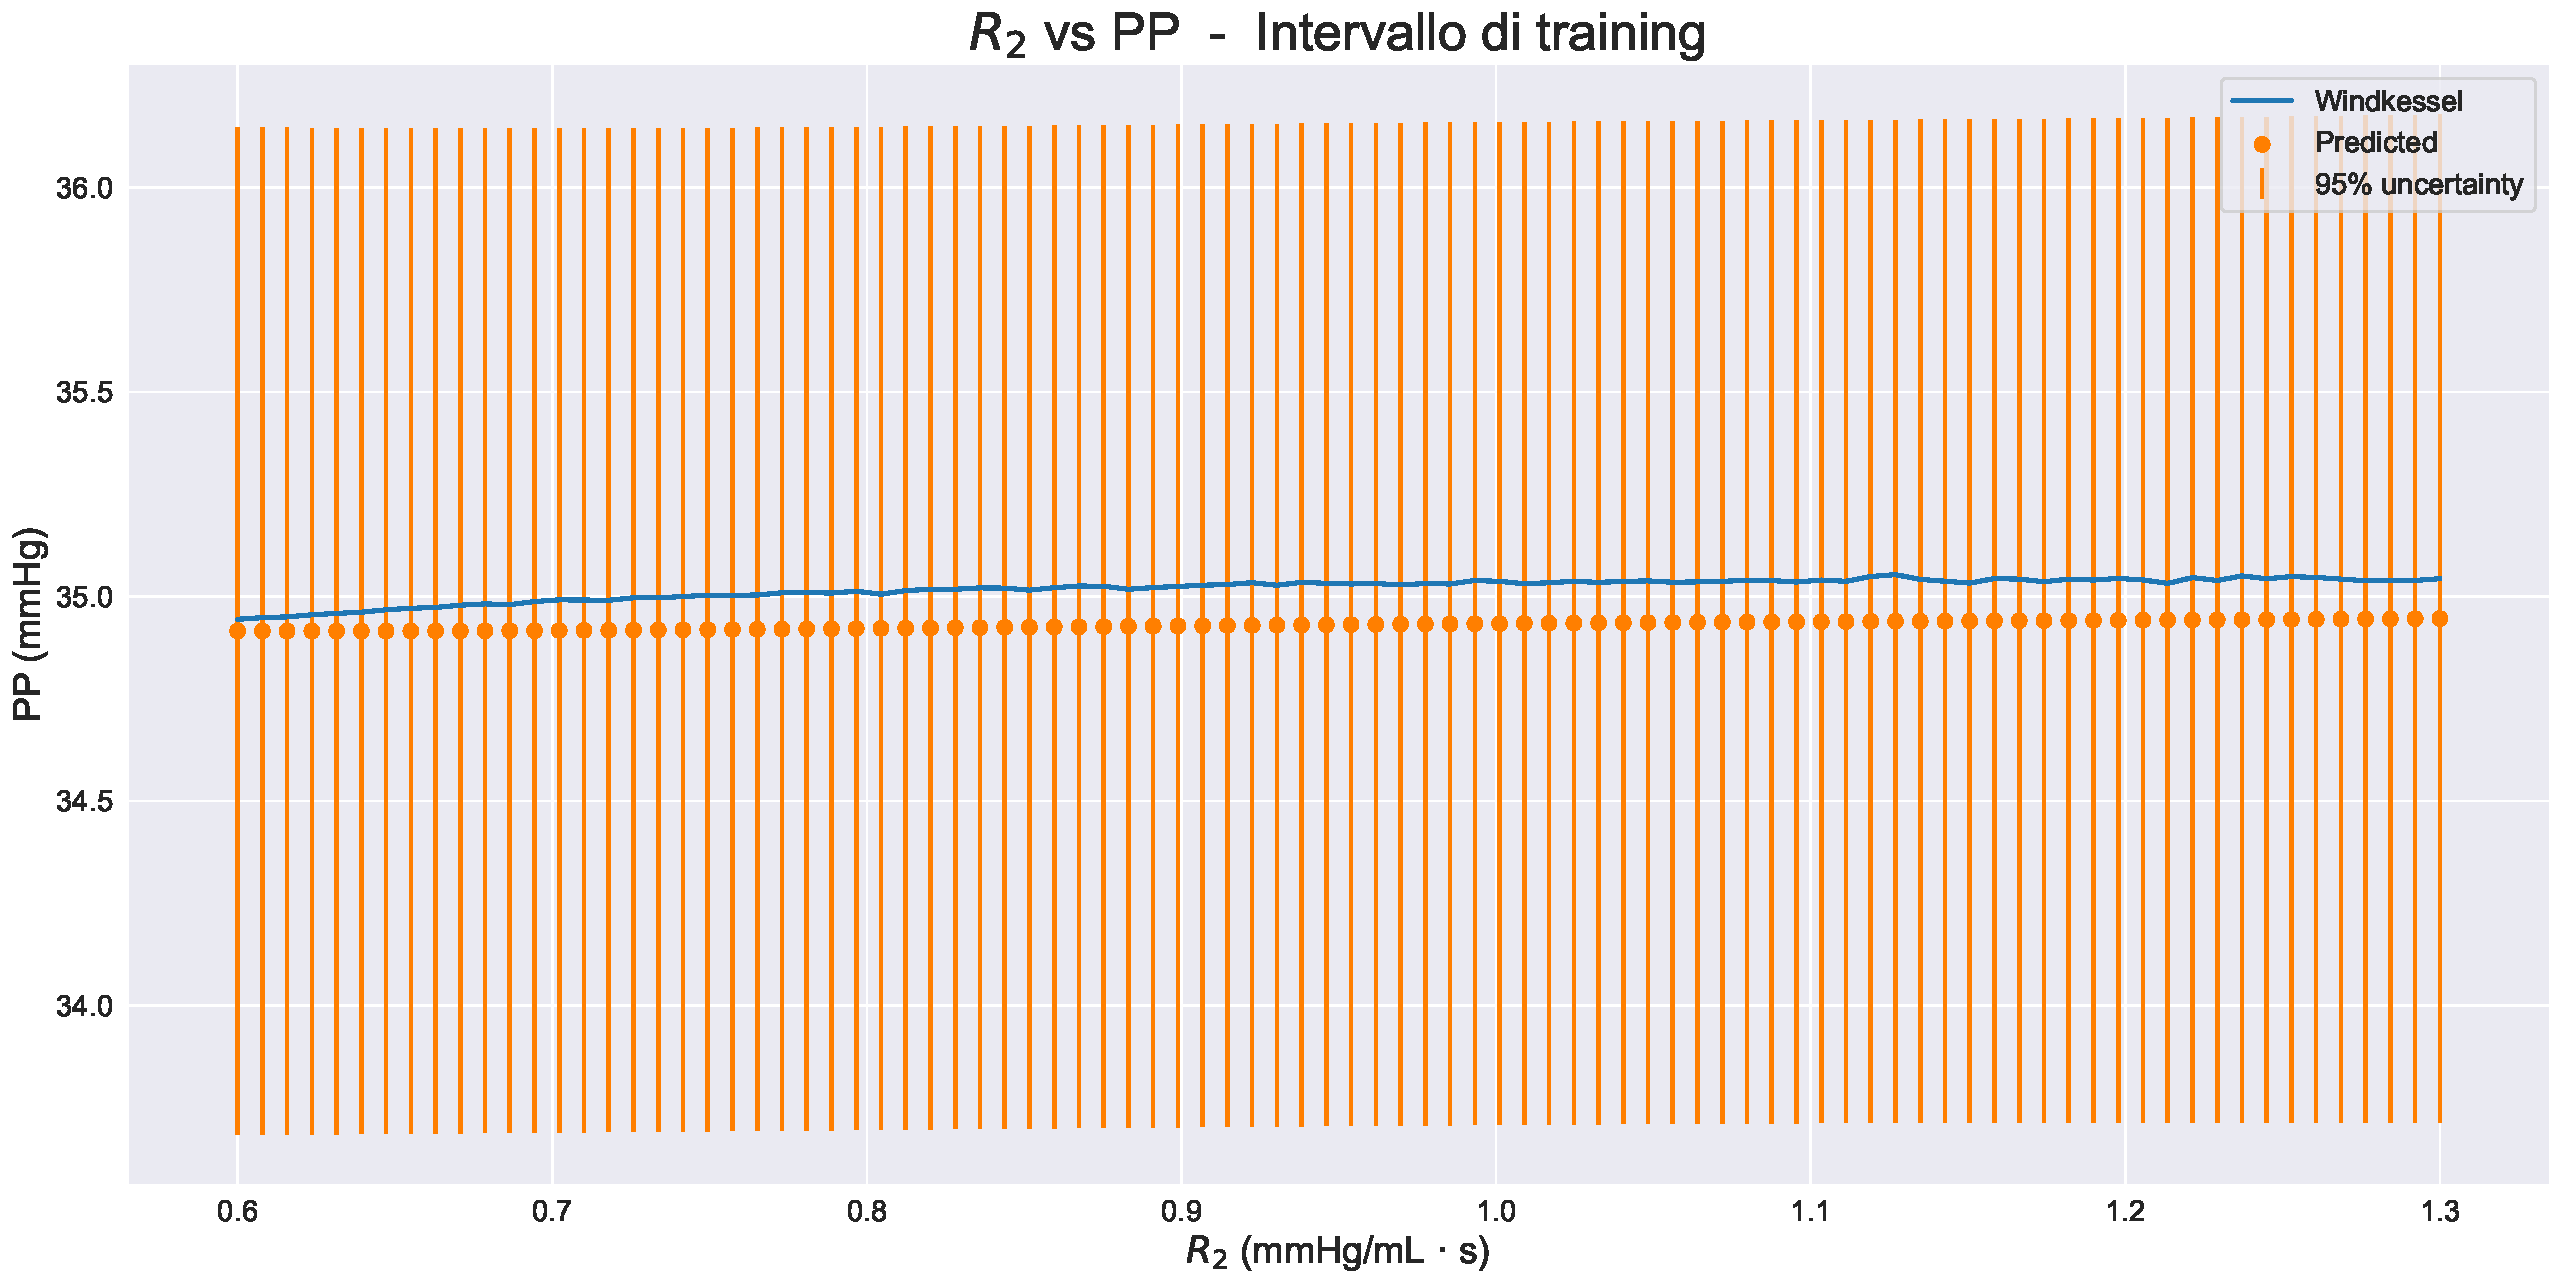
\includegraphics[width=1\textwidth]{images/Training (risultati)/PP/PP - R2 - training.pdf}
    \caption{Dipendenza di PP da $R2$ sull'intervallo di training.}
    \label{PP - R2 - training}
\end{figure}

\begin{figure}
    \centering
    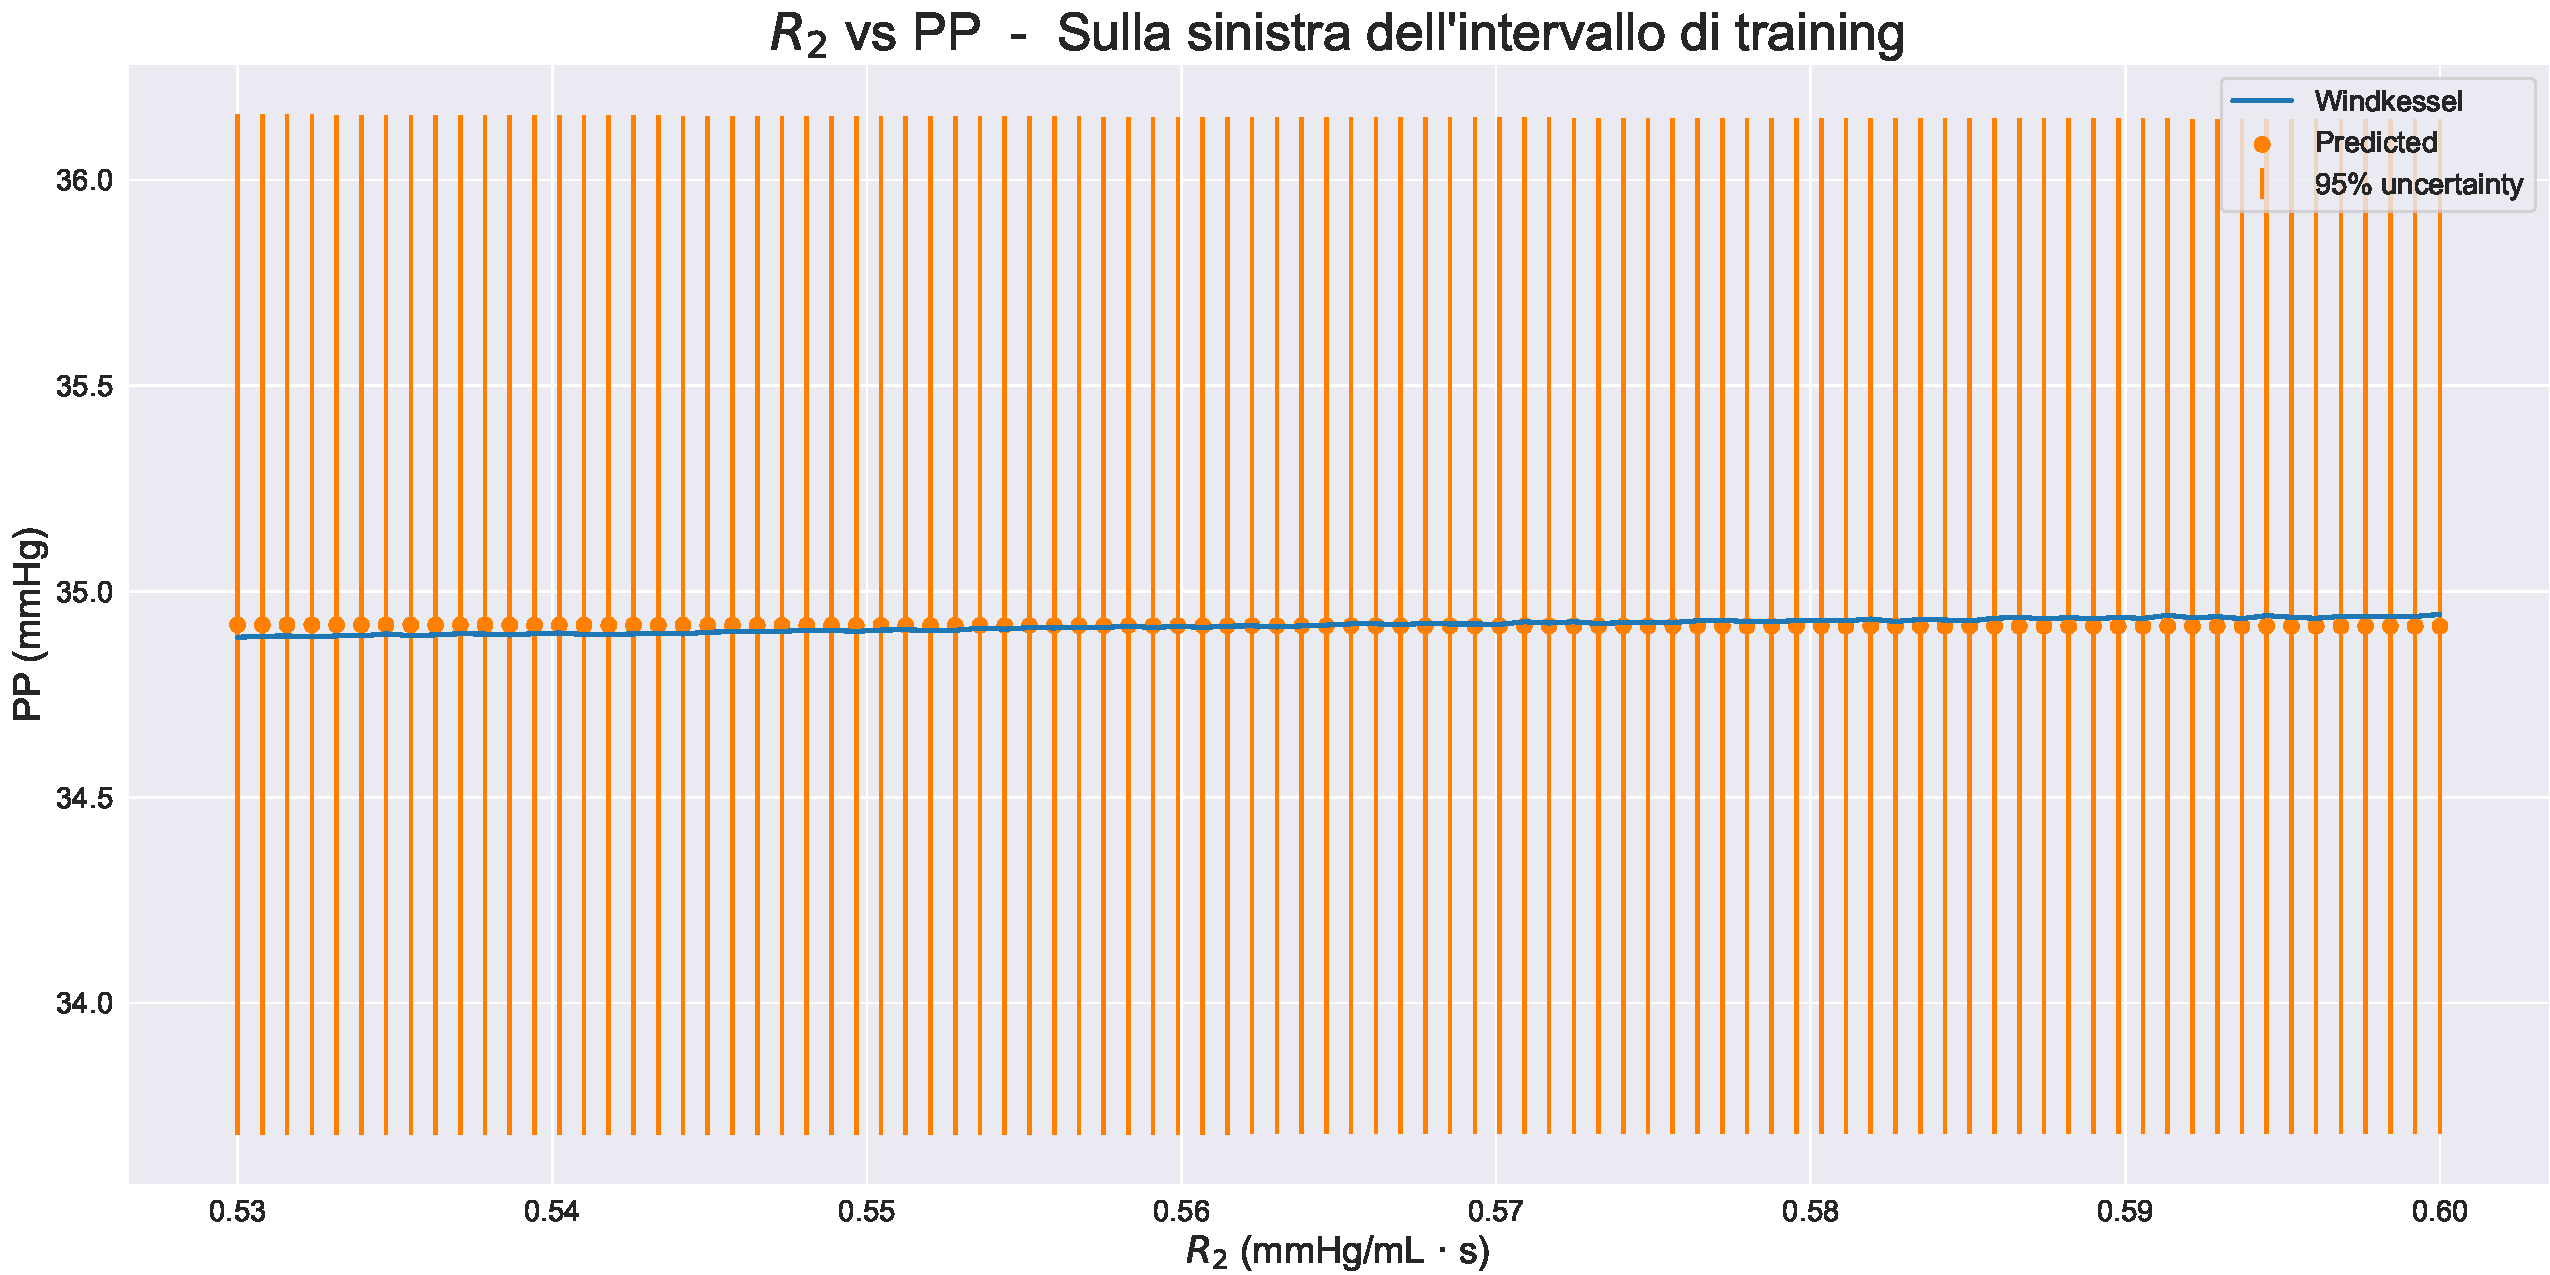
\includegraphics[width=1\textwidth]{images/Training (risultati)/PP/PP - R2 - sx.pdf}
    \caption{Dipendenza di PP da $R2$ sull'intervallo attiguo a sinistra dell'intervallo di training.}
    \label{PP - R2 - sx}
\end{figure}



\begin{figure}
    \centering
    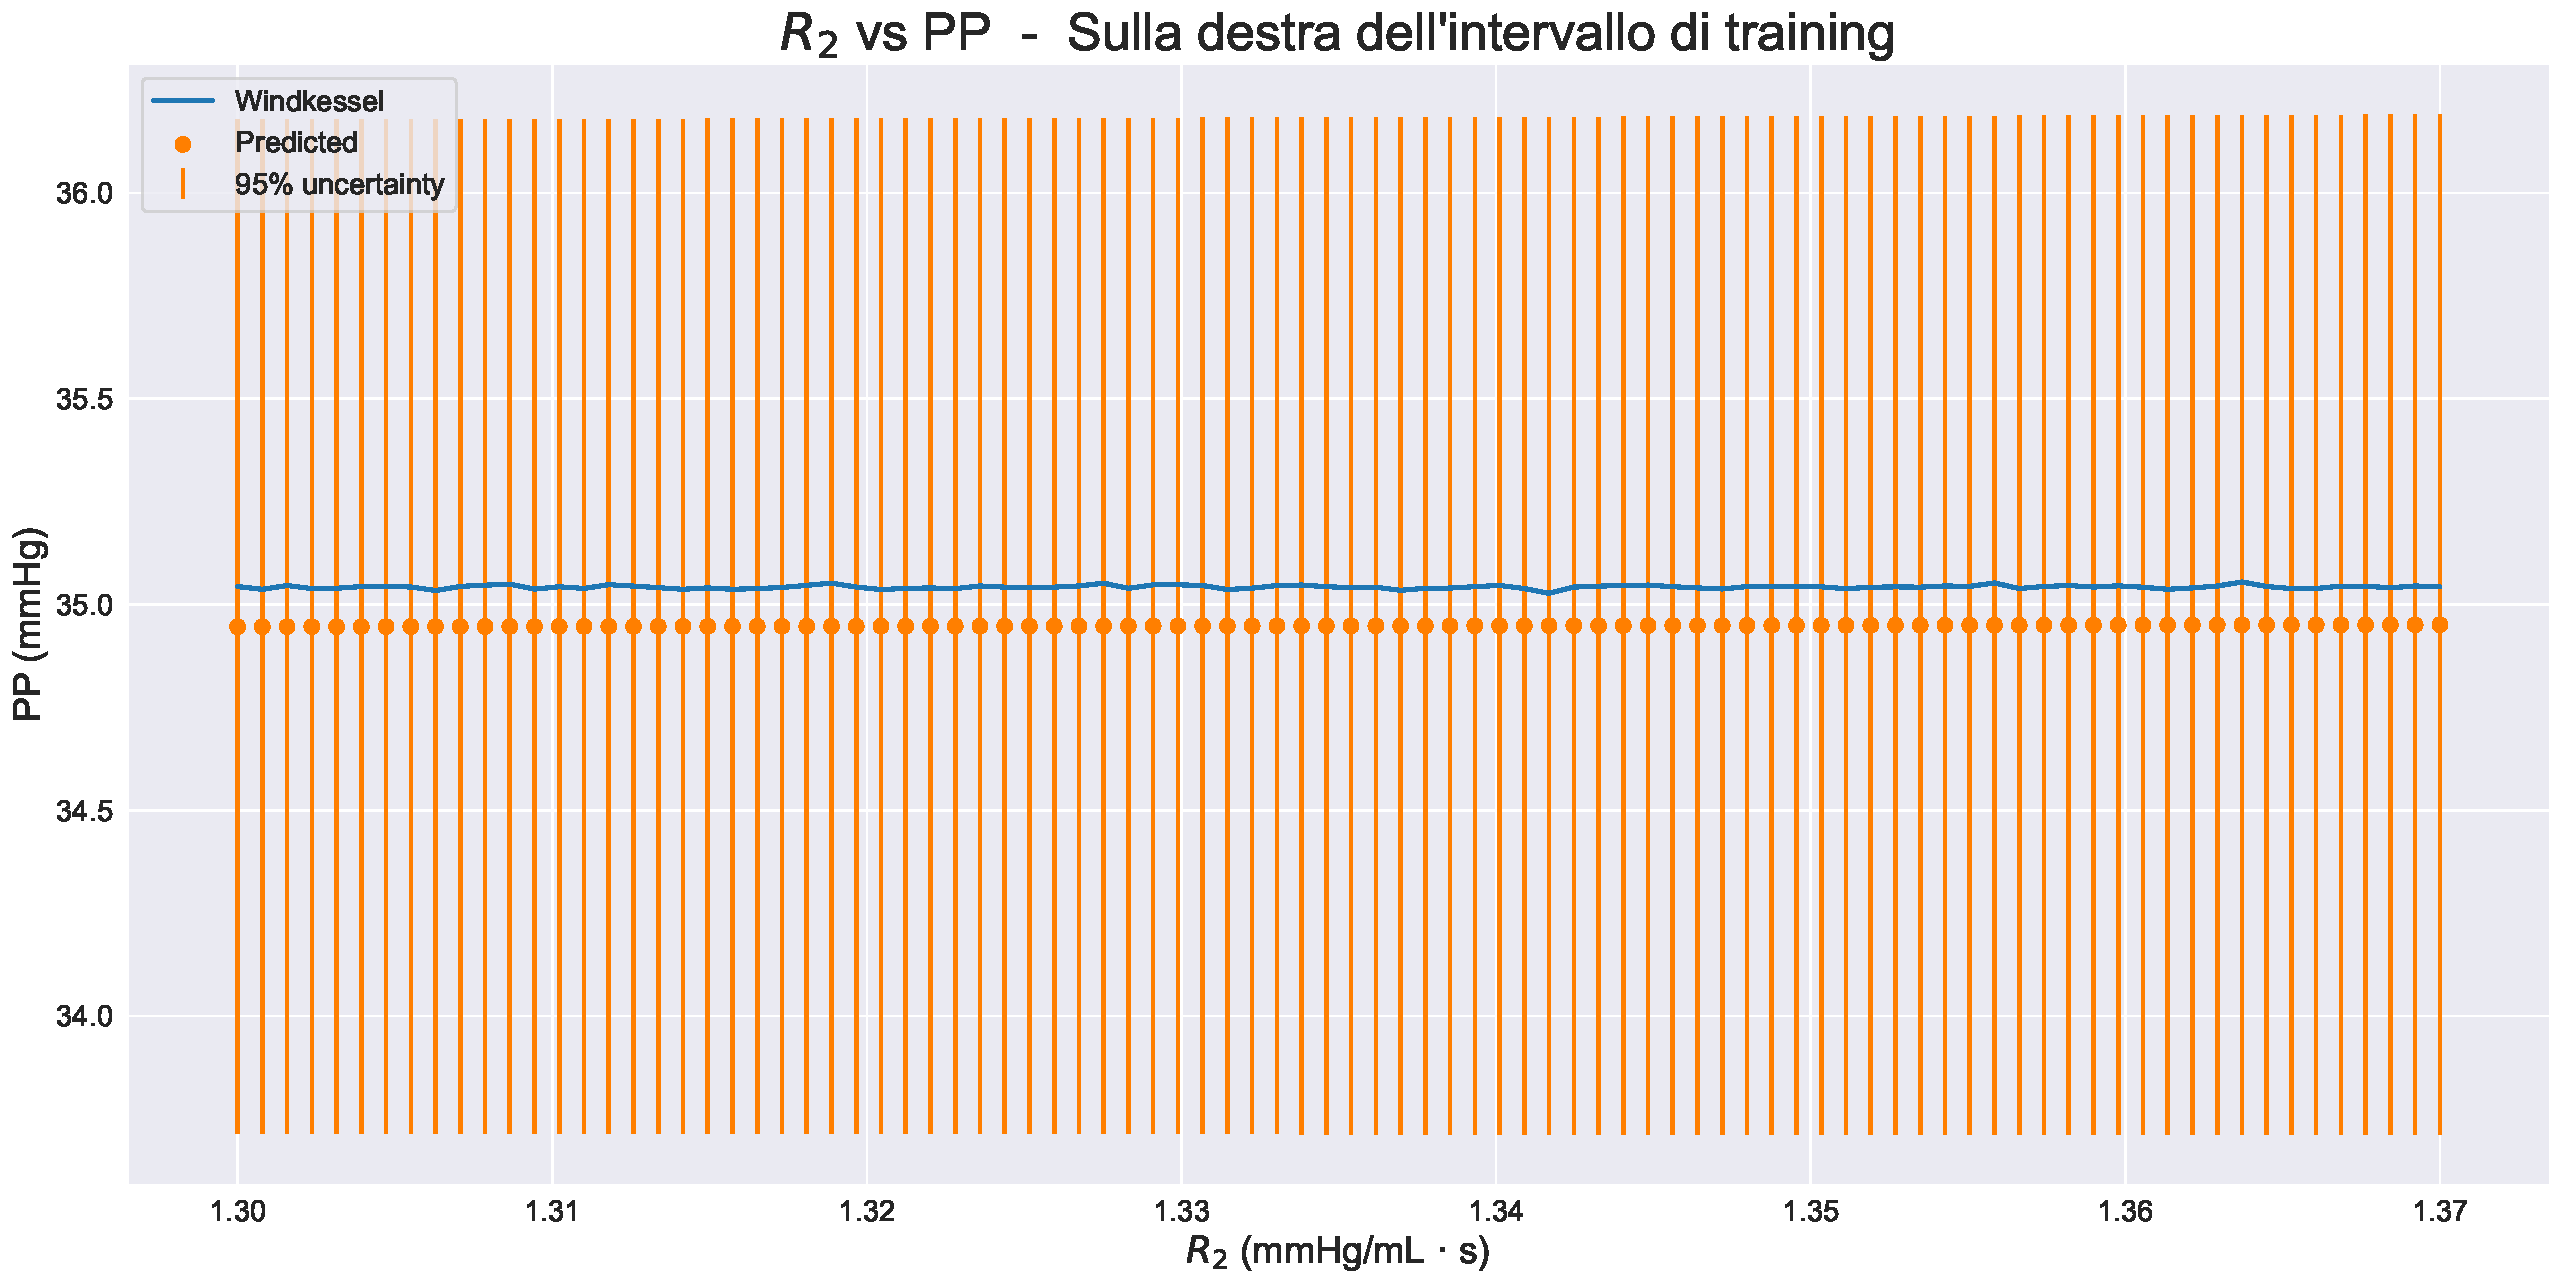
\includegraphics[width=1\textwidth]{images/Training (risultati)/PP/PP - R2 - dx.pdf}
    \caption{Dipendenza di PP da $R2$ sull'intervallo attiguo a destra dell'intervallo di training.}
    \label{PP - R2 - dx}
\end{figure}







\newpage

%******************************
%*********** SBP **************
%******************************
\subsection{Systolic blood pressure (SBP)}
Viene imposto $\text{lr}=0.07$ e viene usato l'early stopper \textit{GLEarlyStoppingCriterion} con parametri: $\alpha = 5$, $\text{patience}=1$.

% **********
% SBP - loss
% **********
\subsubsection{Training e validation loss}
Il training ha necessitato centotredici EPOCHS, ha concluso con $\text{R2Score}=0.9999$, $\text{MeanSquaredError}=0.0052$. In figura \ref{SBP - loss} viene mostrato l'andamento del training e validation loss con MSE e R2Score; in verde l'andamento dell'early stopper.
\begin{figure}[h]
    \centering
    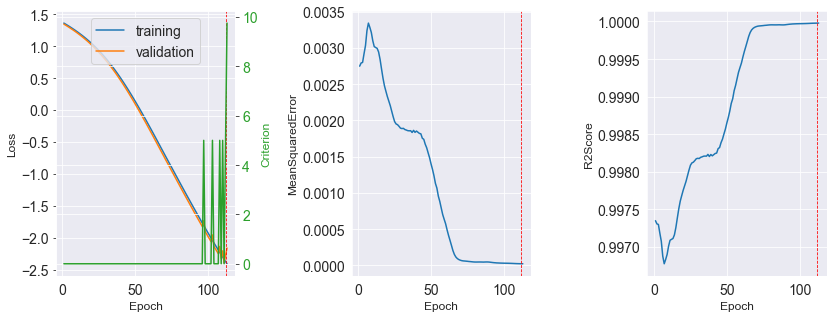
\includegraphics[width=1\textwidth]{images/Training (risultati)/SBP/SBP - loss.png}
    \caption{SBP: andamento del training e validation loss, early stopper, R2Score e MSE.}
    \label{SBP - loss}
\end{figure}

\vspace{-0.5cm}

% **********
% SBP - inference
% **********
\subsubsection{Approssimazione dei dati di input}
In figura \ref{SBP - inference} viene mostrato come le predizioni approssimano i dati di input. Le barre di errore sono lunghe $0.0012$, dunque non si notano.

\begin{figure}[h]
    \centering
    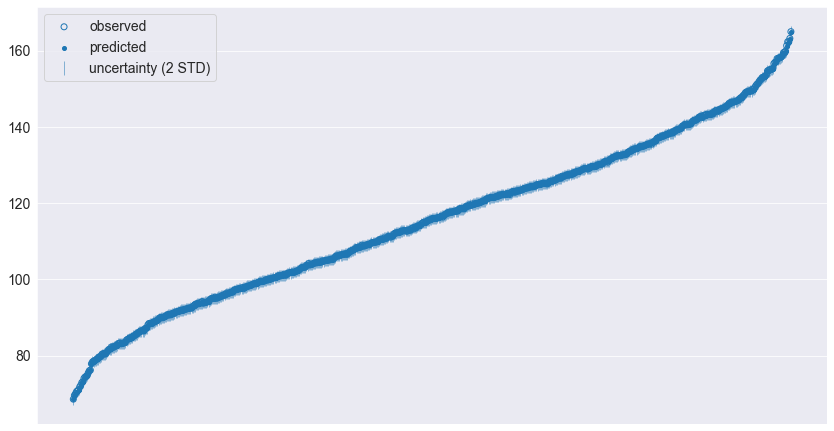
\includegraphics[width=1\textwidth]{images/Training (risultati)/SBP/SBP - inference.png}
    \caption{SBP: predizioni sui dati di input.}
    \label{SBP - inference}
\end{figure}



% **********
% SBP - C
% **********
\subsubsection{Dipendenza da $C$}
Il risultato complessivo è mostrato in figura \ref{SBP - C - full}, il risultato nel solo intervallo di training in \ref{SBP - C - training}, il risultato nei singoli intervalli attigui in \ref{SBP - C - sx} e \ref{SBP - C - dx}.

\vspace{1cm}

\begin{figure}[!htb]
    \centering
    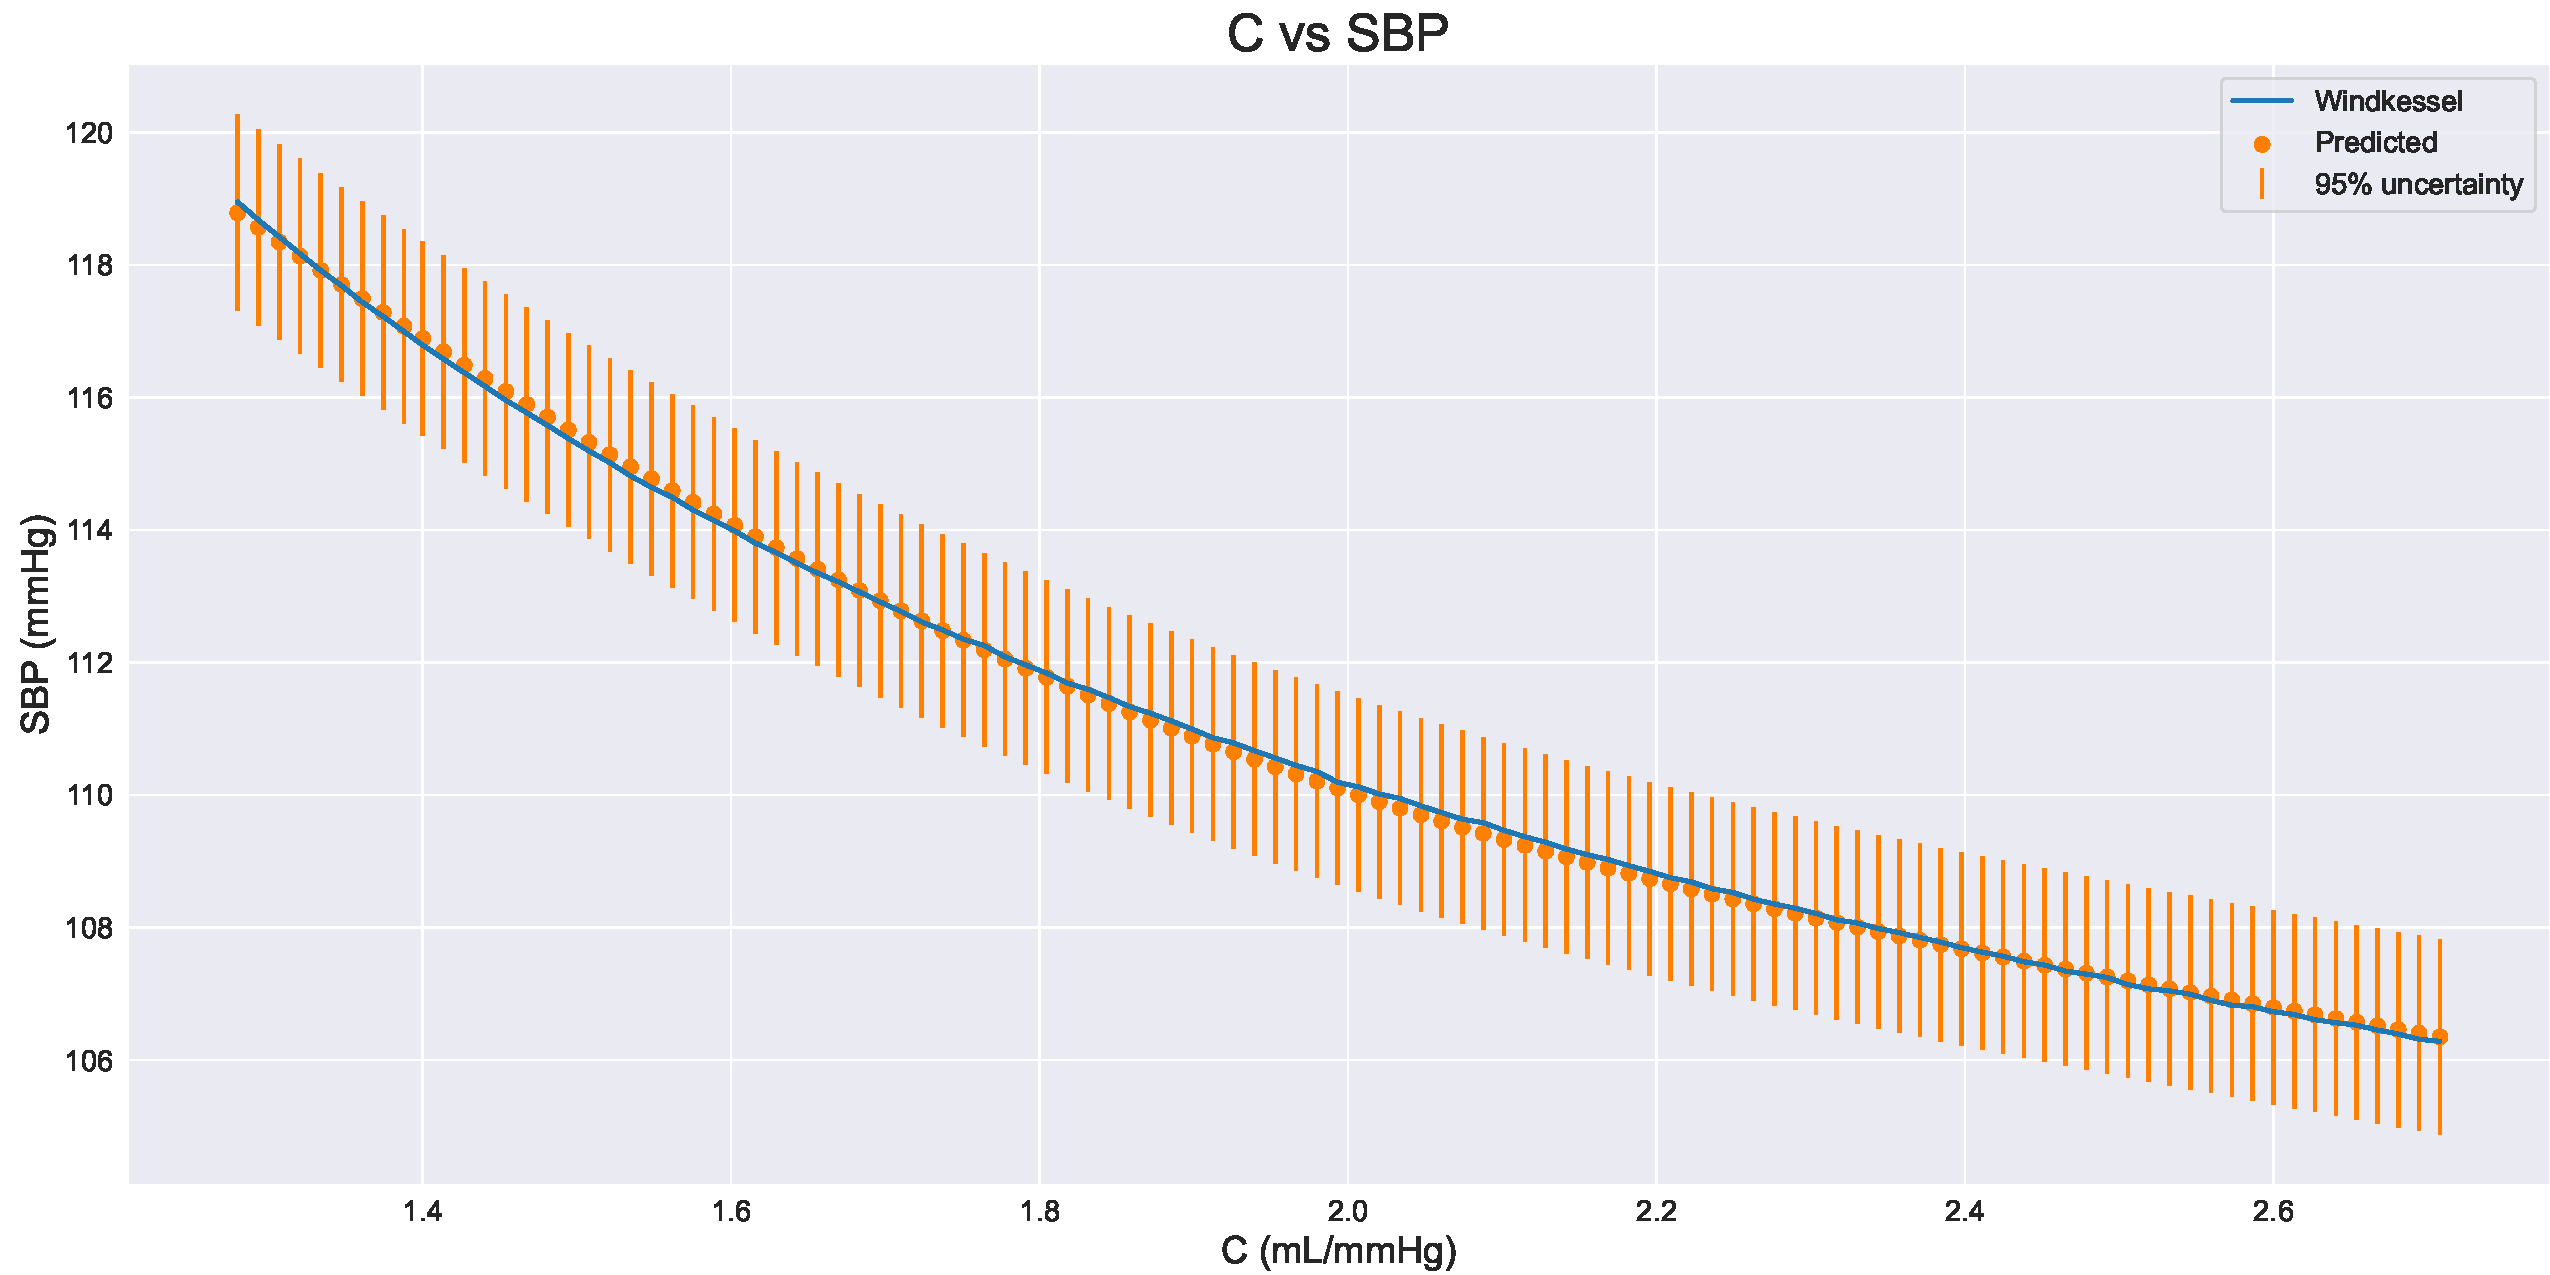
\includegraphics[width=1\textwidth]{images/Training (risultati)/SBP/SBP - C - full.pdf}
    \caption{Dipendenza di SBP da $C$ sull'intervallo di training e due intervalli attigui.}
    \label{SBP - C - full}
\end{figure}

\vspace{0.32cm}

\begin{figure}[!htb]
    \centering
    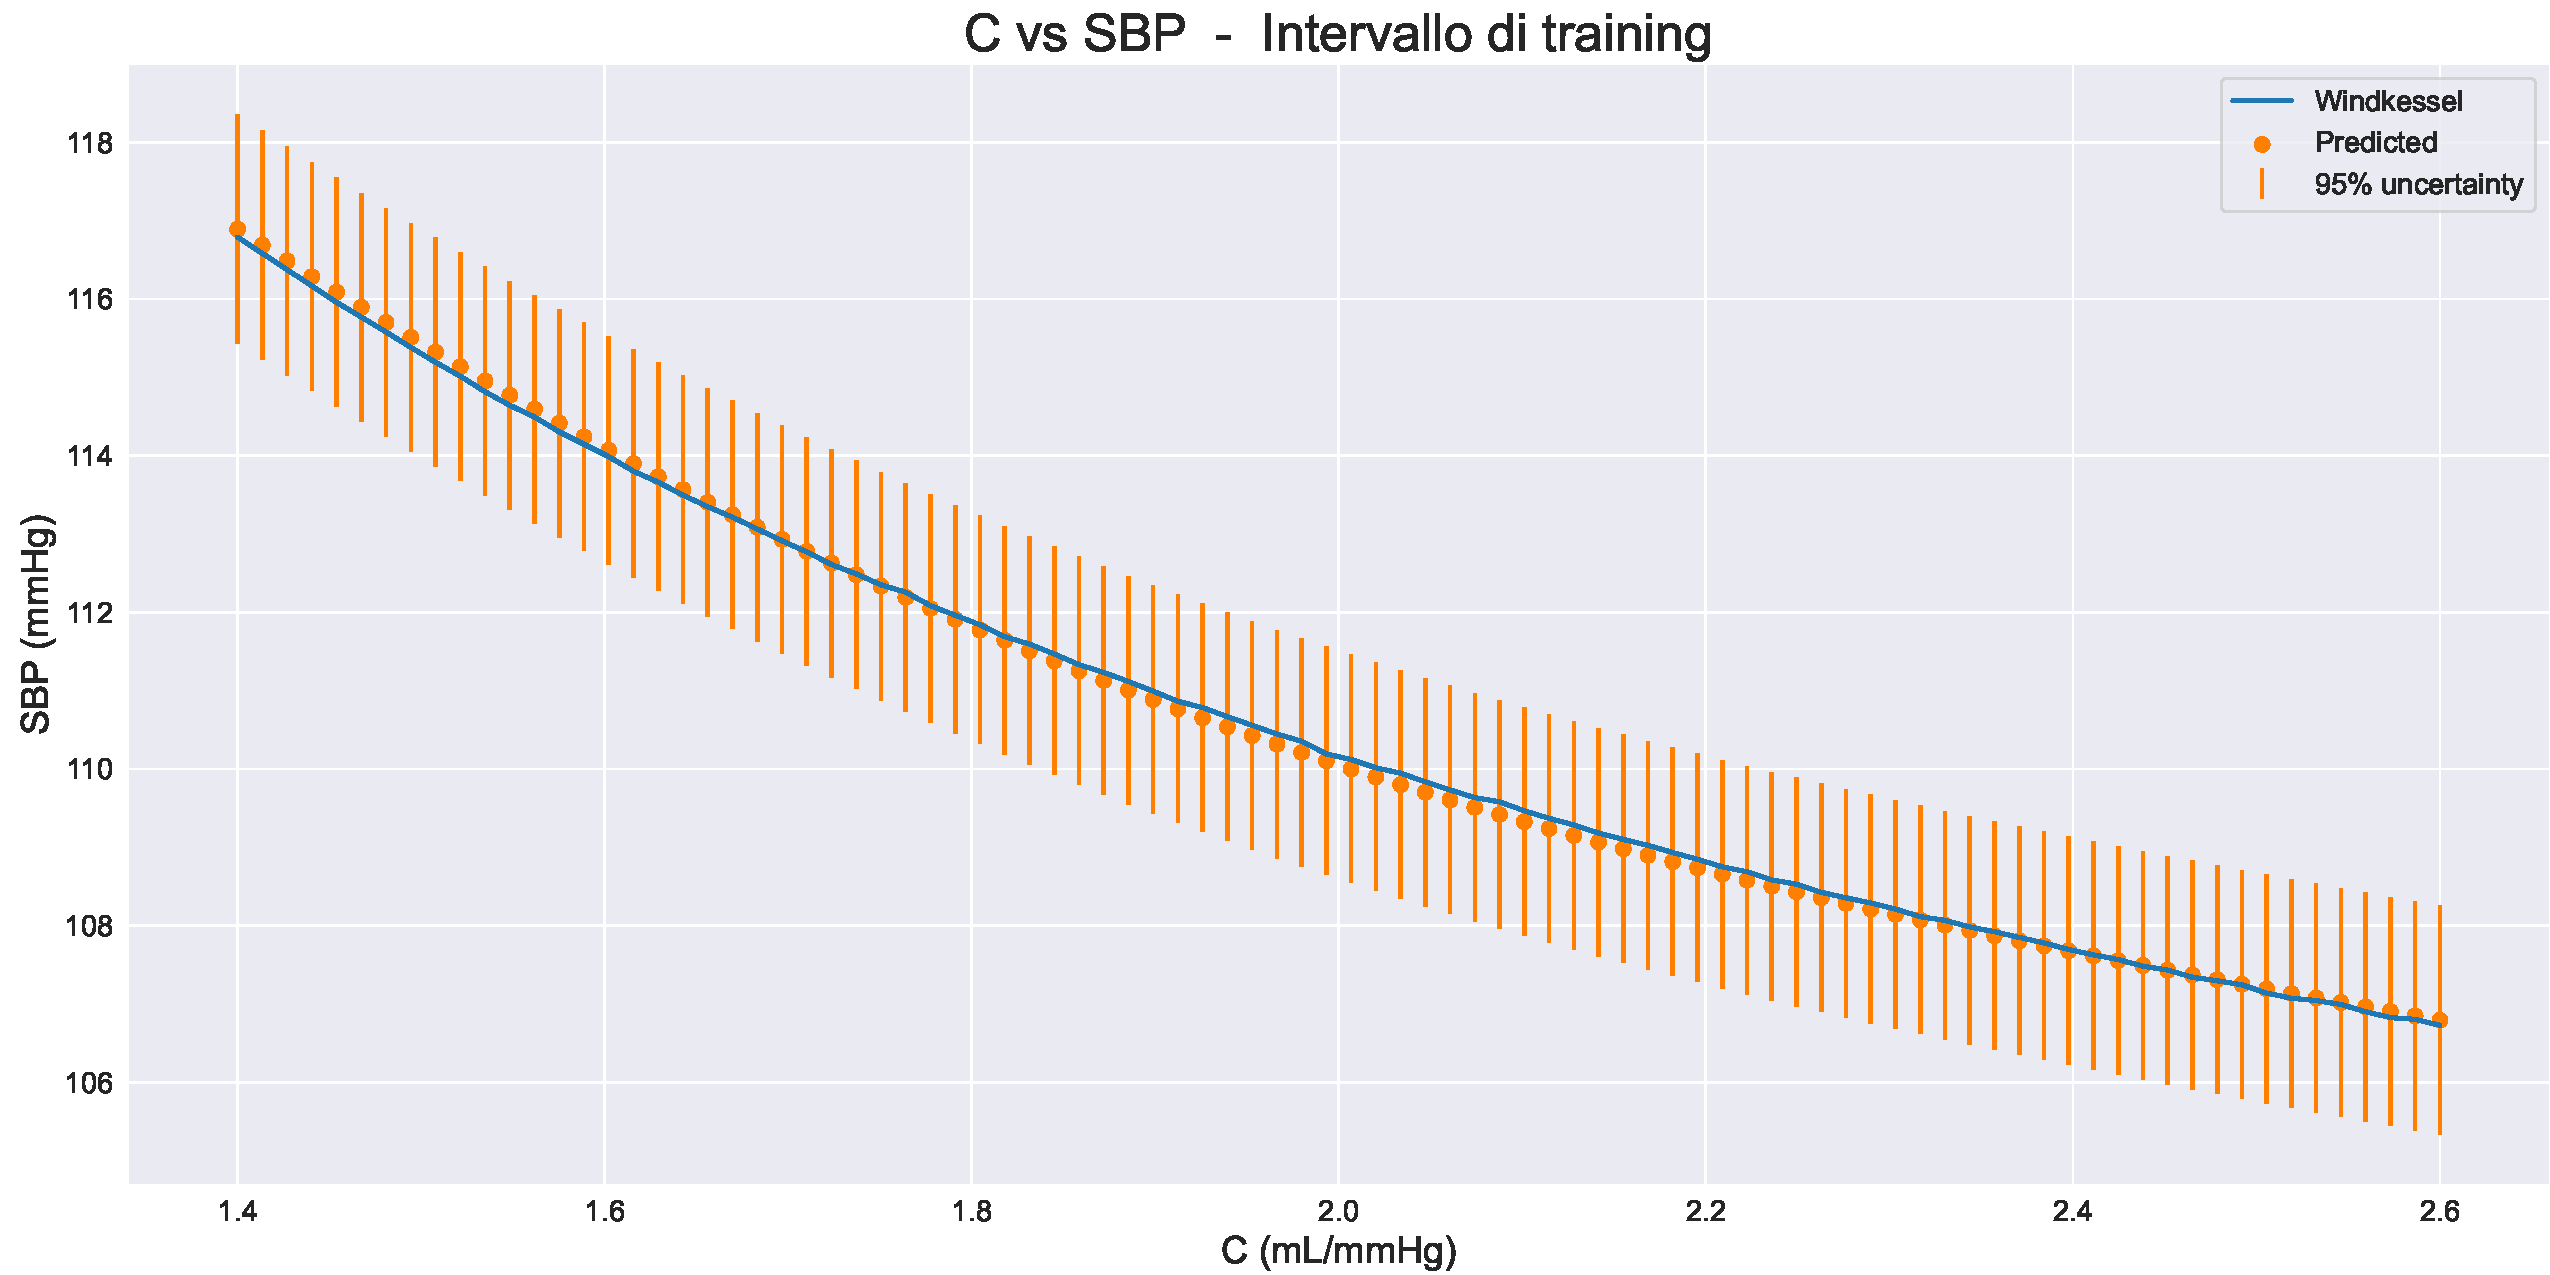
\includegraphics[width=1\textwidth]{images/Training (risultati)/SBP/SBP - C - training.pdf}
    \caption{Dipendenza di SBP da $C$ sull'intervallo di training.}
    \label{SBP - C - training}
\end{figure}

\begin{figure}
    \centering
    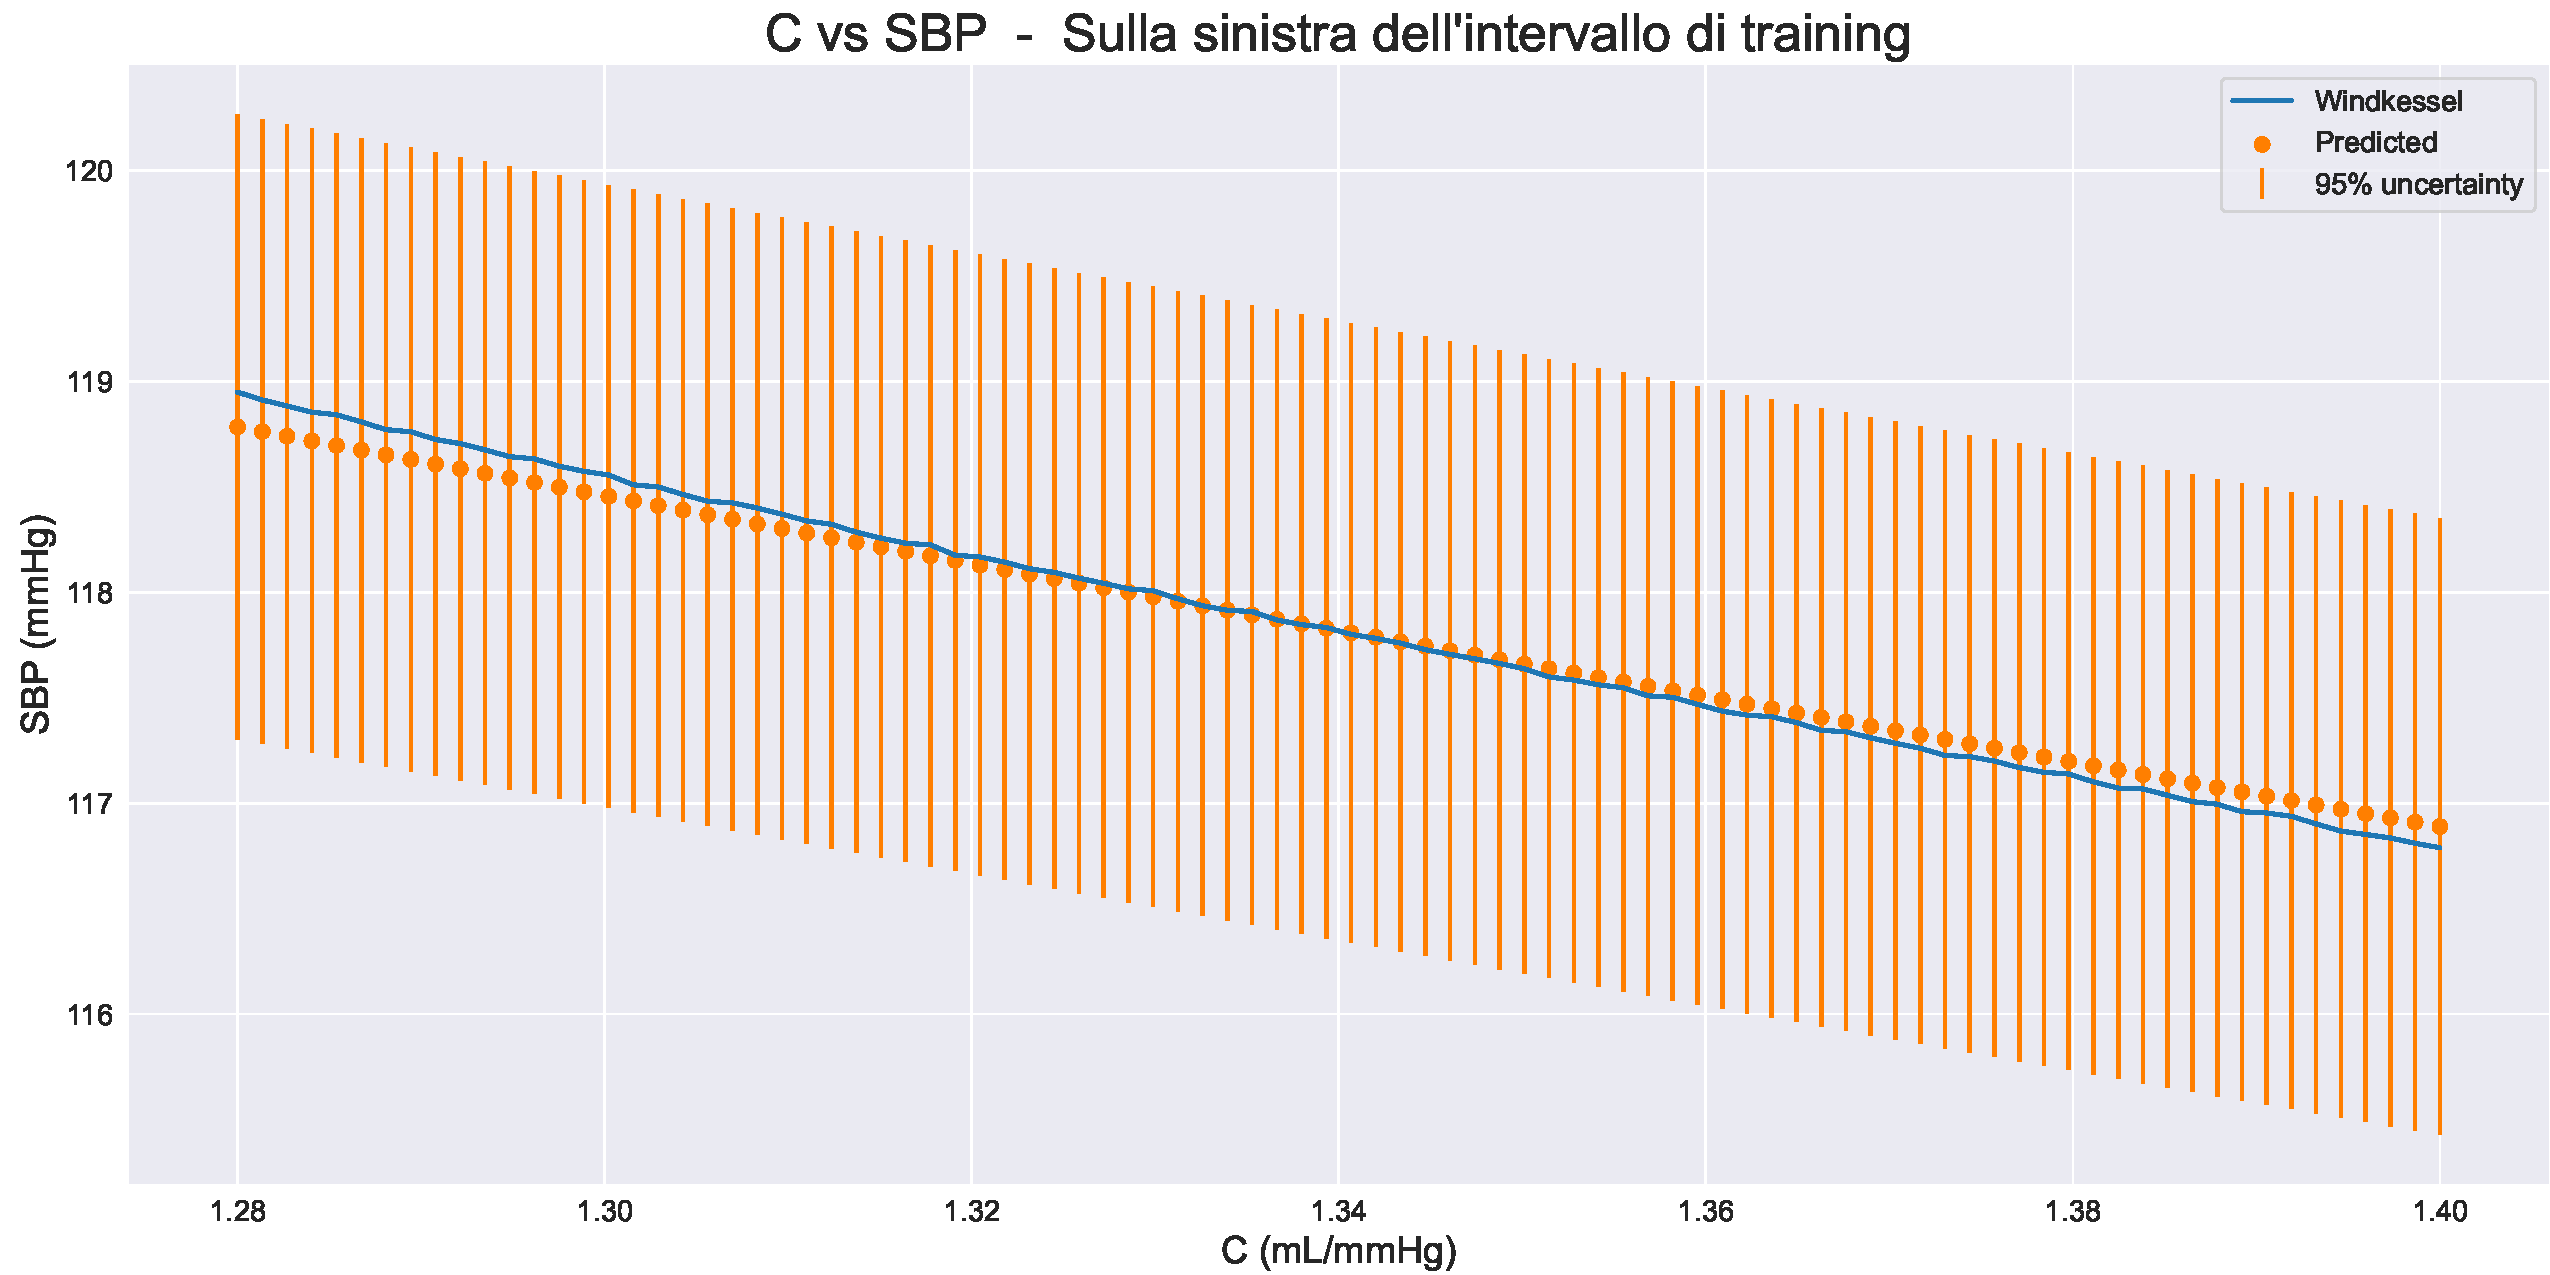
\includegraphics[width=1\textwidth]{images/Training (risultati)/SBP/SBP - C - sx.pdf}
    \caption{Dipendenza di SBP da $C$ sull'intervallo attiguo a sinistra dell'intervallo di training.}
    \label{SBP - C - sx}
\end{figure}


\begin{figure}
    \centering
    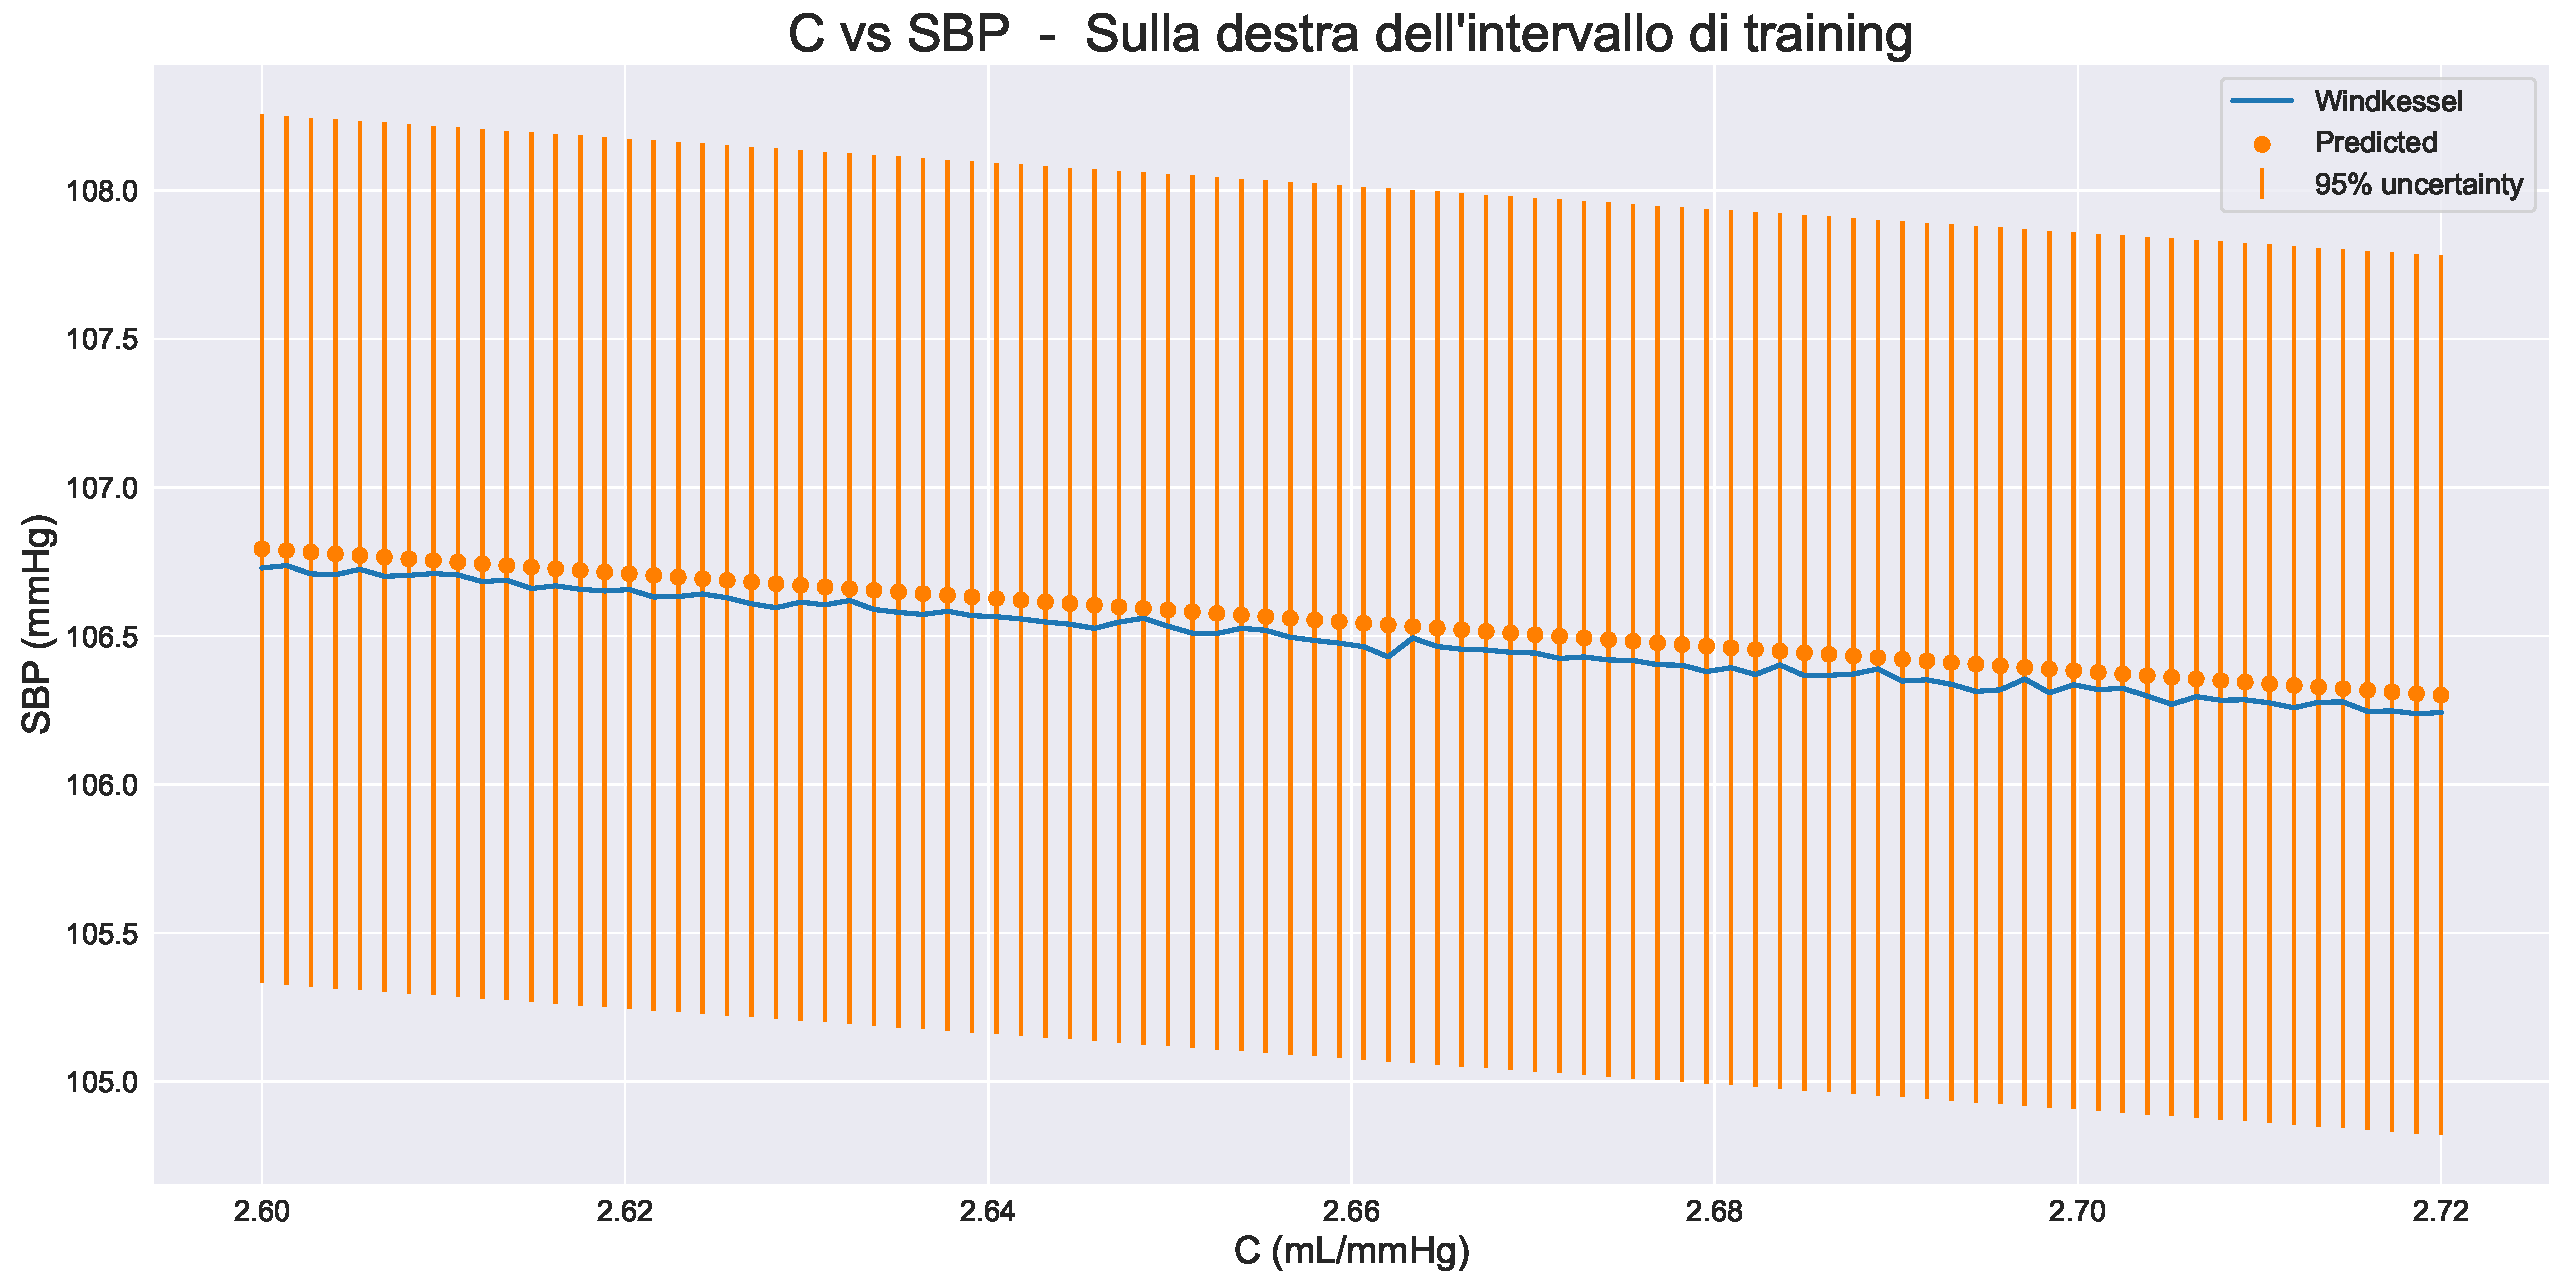
\includegraphics[width=1\textwidth]{images/Training (risultati)/SBP/SBP - C - dx.pdf}
    \caption{Dipendenza di SBP da $C$ sull'intervallo attiguo a destra dell'intervallo di training.}
    \label{SBP - C - dx}
\end{figure}



\newpage

% **********
% SBP - R1
% **********
\subsubsection{Dipendenza da $R_1$}
Il risultato complessivo è mostrato in figura \ref{SBP - R1 - full}, il risultato nel solo intervallo di training in \ref{SBP - R1 - training}, il risultato nei singoli intervalli attigui in \ref{SBP - R1 - sx} e \ref{SBP - R1 - dx}.

\vspace{0.7cm}


\begin{figure}[!htb]
    \centering
    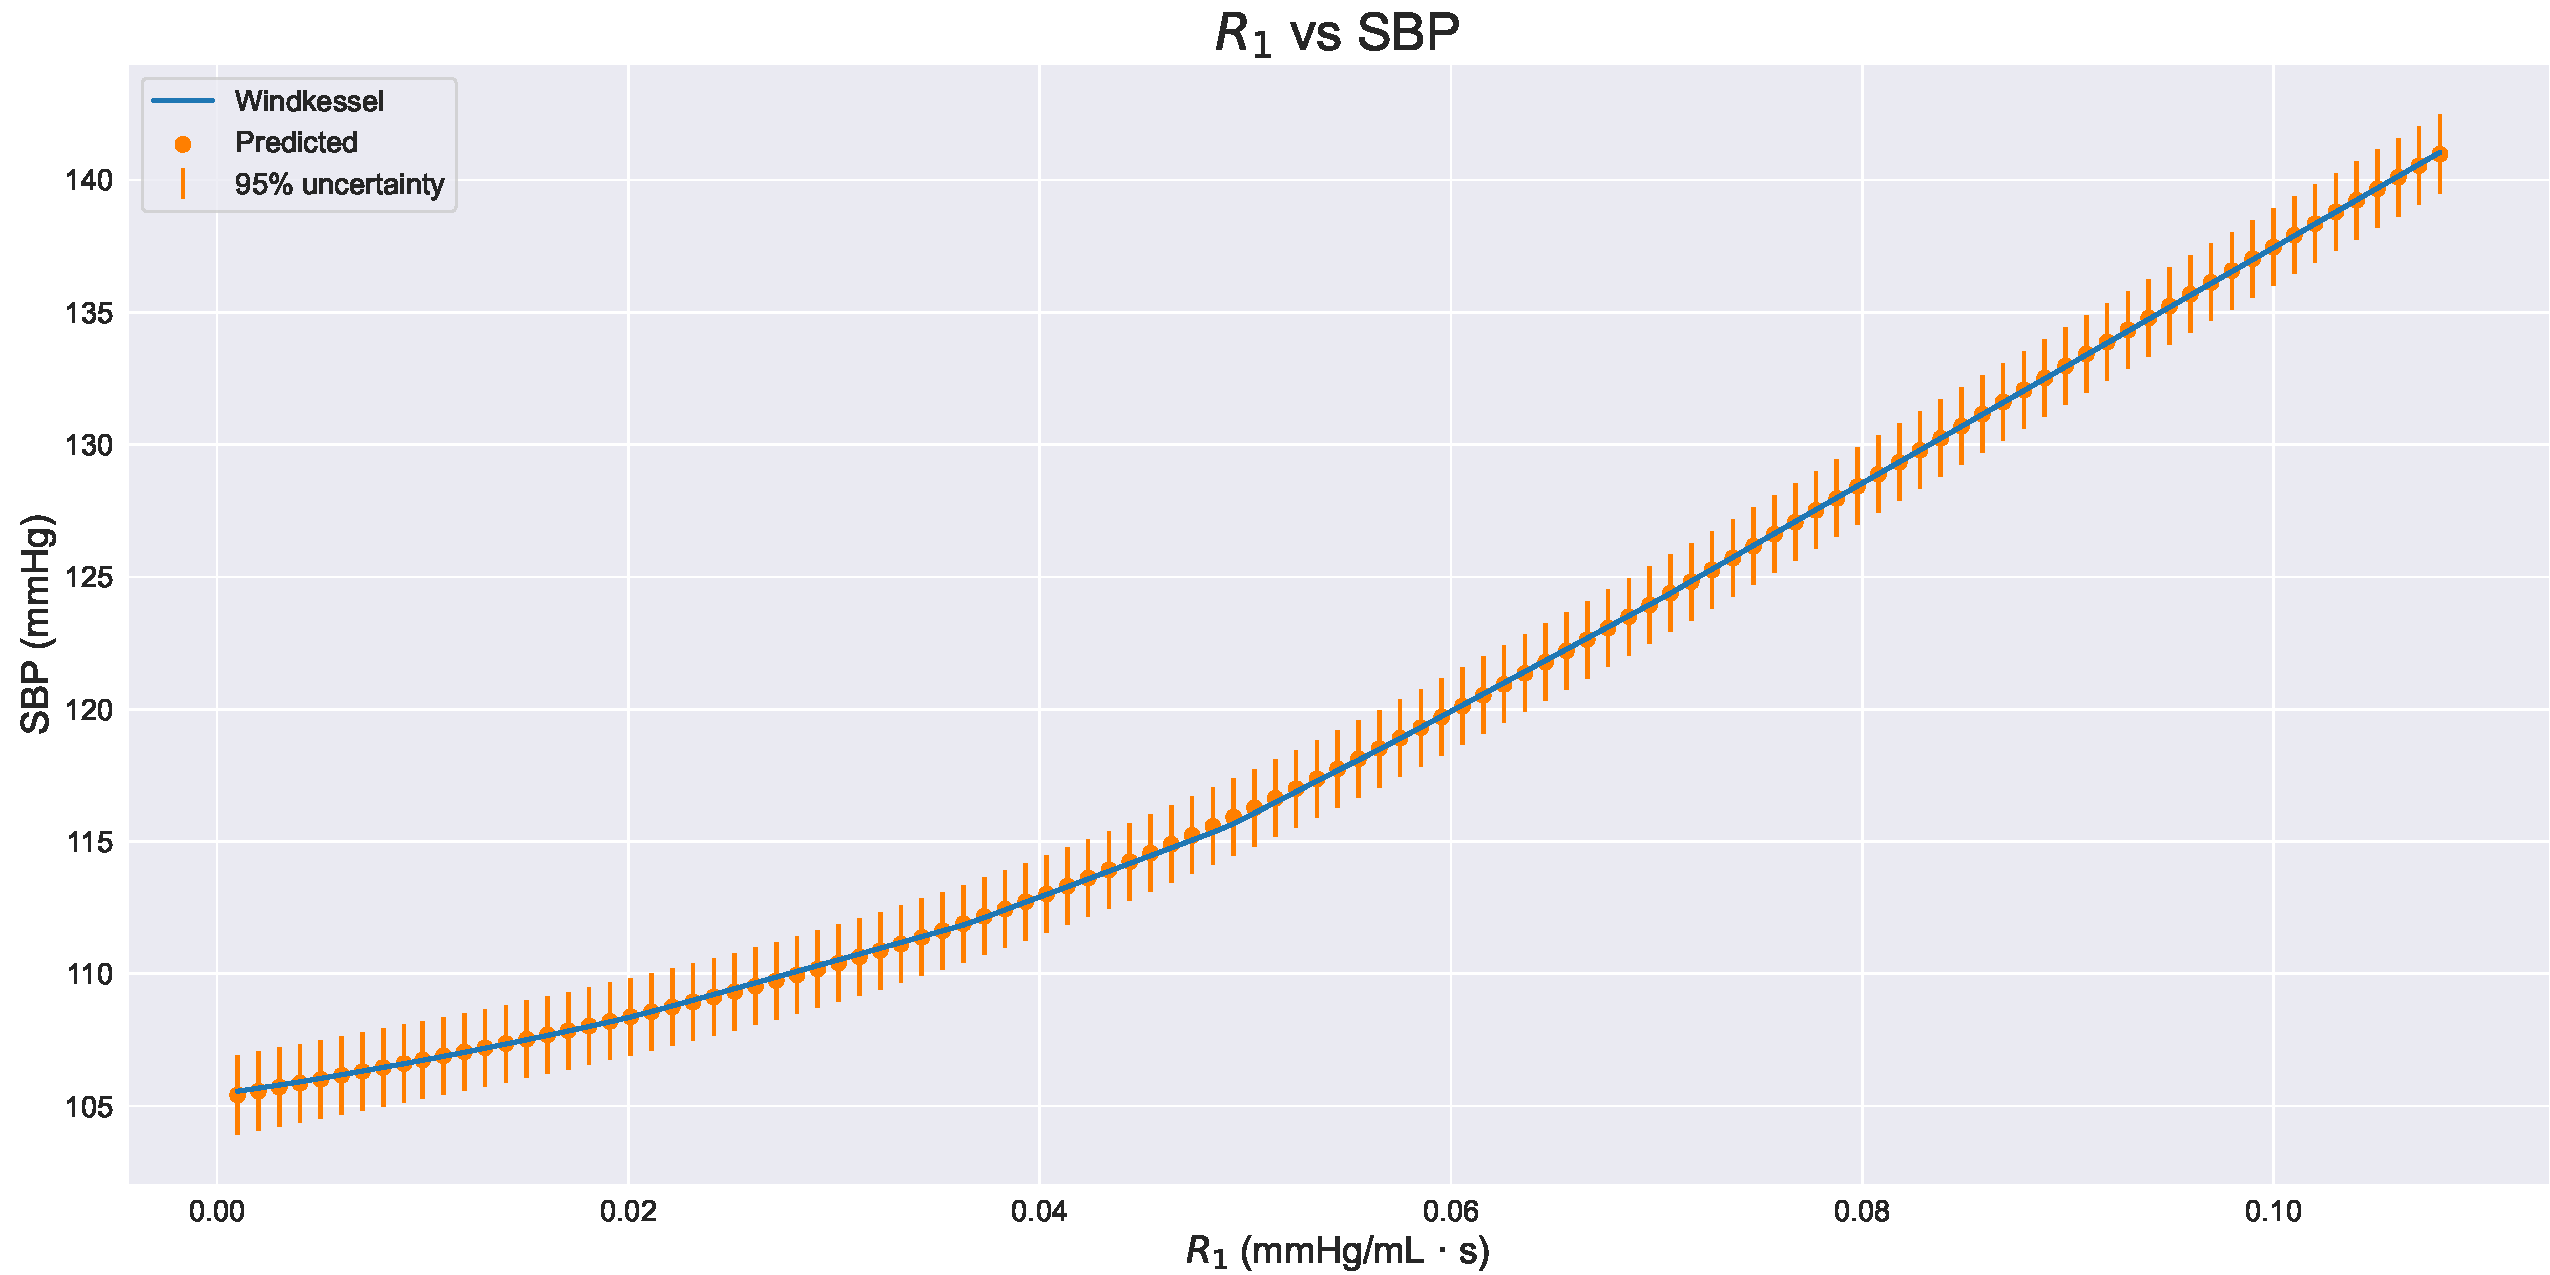
\includegraphics[width=1\textwidth]{images/Training (risultati)/SBP/SBP - R1 - full.pdf}
    \caption{Dipendenza di SBP da $R1$ sull'intervallo di training e due intervalli attigui.}
    \label{SBP - R1 - full}
\end{figure}

\vspace{0.32cm}

\begin{figure}[!htb]
    \centering
    \includegraphics[width=1\textwidth]{images/Training (risultati)/SBP/SBP - R1 - training.pdf}
    \caption{Dipendenza di SBP da $R1$ sull'intervallo di training.}
    \label{SBP - R1 - training}
\end{figure}

\begin{figure}
    \centering
    \includegraphics[width=1\textwidth]{images/Training (risultati)/SBP/SBP - R1 - sx.pdf}
    \caption{Dipendenza di SBP da $R1$ sull'intervallo attiguo a sinistra dell'intervallo di training.}
    \label{SBP - R1 - sx}
\end{figure}



\begin{figure}
    \centering
    \includegraphics[width=1\textwidth]{images/Training (risultati)/SBP/SBP - R1 - dx.pdf}
    \caption{Dipendenza di SBP da $R1$ sull'intervallo attiguo a destra dell'intervallo di training.}
    \label{SBP - R1 - dx}
\end{figure}






\newpage
% **********
% SBP - R2
% **********
\subsubsection{Dipendenza da $R_2$}
Il risultato complessivo è mostrato in figura \ref{SBP - R2 - full}, il risultato nel solo intervallo di training in \ref{SBP - R2 - training}, il risultato nei singoli intervalli attigui in \ref{SBP - R2 - sx} e \ref{SBP - R2 - dx}.

\vspace{1cm}

\begin{figure}[!htb]
    \centering
    \includegraphics[width=1\textwidth]{images/Training (risultati)/SBP/SBP - R2 - full.pdf}
    \caption{Dipendenza di SBP da $R2$ sull'intervallo di training e due intervalli attigui.}
    \label{SBP - R2 - full}
\end{figure}

\vspace{0.32cm}

\begin{figure}[!htb]
    \centering
    \includegraphics[width=1\textwidth]{images/Training (risultati)/SBP/SBP - R2 - training.pdf}
    \caption{Dipendenza di SBP da $R2$ sull'intervallo di training.}
    \label{SBP - R2 - training}
\end{figure}

\begin{figure}
    \centering
    \includegraphics[width=1\textwidth]{images/Training (risultati)/SBP/SBP - R2 - sx.pdf}
    \caption{Dipendenza di SBP da $R2$ sull'intervallo attiguo a sinistra dell'intervallo di training.}
    \label{SBP - R2 - sx}
\end{figure}



\begin{figure}
    \centering
    \includegraphics[width=1\textwidth]{images/Training (risultati)/SBP/SBP - R2 - dx.pdf}
    \caption{Dipendenza di SBP da $R2$ sull'intervallo attiguo a destra dell'intervallo di training.}
    \label{SBP - R2 - dx}
\end{figure}

\section{Tempo di esecuzione: approssimazione di MAP, DBP, SBP, PP}
Come fatto in \ref{Windkessel: tempo esecuzione}, si calcola ora il tempo di esecuzione per trovare il valore di MAP, DBP, SBP, PP a partire dai valori di $C, R_1, R_2$. Poichè viene eseguito un training per ogni parametro, vengono riportati i tempi di stima dei parametri per ogni modello addestrato.

% Please add the following required packages to your document preamble:
% \usepackage{lscape}

\begin{table}[!htb]
\centering
\begin{tabular}{cc}
\hline
\textbf{Parametro stimato} & \textbf{\begin{tabular}[c]{@{}c@{}}Tempo esecuzione\\ (media + dev. std.)\end{tabular}} \\ \hline
DBP & 5.89 ms ± 1.63 ms \\
SBP & 5.23 ms ± 1.75 ms \\
MAP & 5.6 ms ± 1.64 ms  \\
PP  & 4.03 ms ± 1.19 ms \\ \hline
\end{tabular}
\caption{Tempo di esecuzione per trovare l’approssimazione dei parametri usando i processi gaussiani addestrati.}
\label{tab: tempo par}
\end{table}


Poichè per ogni parametro si addestra un modello indipendente, per ottenere i valori di MAP, DBP, SBP e PP è necessario girare i quattro processi gaussiani addestrati. Dunque il tempo di esecuzione necessario per ottenere le approssimazioni dei quattro parametri è la somma dei tempi necessari per ottenerli uno a uno. Dunque si può dire che in tutto sono necessari 20.75 ms in media per ottenere i quattro valori.
Comparando questa quantità alla tabella \ref{tab: tempo windkessel} è evidente che l'uso dei processi gaussiani richiede molto meno tempo rispetto all'approssimazione della soluzione del modello Windkessel già dopo soli dieci cicli cardiaci (un numero piuttosto basso se l'obiettivo è trovare la soluzione a convergenza). \\


Evidentemente, dunque, i processi gaussiani risolvono il problema del tempo di esecuzione nel modello Windkessel, fornendo una buona approssimazione del valore di MAP, DBP, SBP, PP.
